%Version 3.1 December 2024
% See section 11 of the User Manual for version history
%
%%%%%%%%%%%%%%%%%%%%%%%%%%%%%%%%%%%%%%%%%%%%%%%%%%%%%%%%%%%%%%%%%%%%%%
%%                                                                 %%
%% Please do not use \input{...} to include other tex files.       %%
%% Submit your LaTeX manuscript as one .tex document.              %%
%%                                                                 %%
%% All additional figures and files should be attached             %%
%% separately and not embedded in the \TeX\ document itself.       %%
%%                                                                 %%
%%%%%%%%%%%%%%%%%%%%%%%%%%%%%%%%%%%%%%%%%%%%%%%%%%%%%%%%%%%%%%%%%%%%%

%%\documentclass[referee,sn-basic]{sn-jnl}% referee option is meant for double line spacing

%%=======================================================%%
%% to print line numbers in the margin use lineno option %%
%%=======================================================%%

%%\documentclass[lineno,pdflatex,sn-basic]{sn-jnl}% Basic Springer Nature Reference Style/Chemistry Reference Style

%%=========================================================================================%%
%% the documentclass is set to pdflatex as default. You can delete it if not appropriate.  %%
%%=========================================================================================%%

%%\documentclass[sn-basic]{sn-jnl}% Basic Springer Nature Reference Style/Chemistry Reference Style

%%Note: the following reference styles support Namedate and Numbered referencing. By default the style follows the most common style. To switch between the options you can add or remove “Numbered” in the optional parenthesis. 
%%The option is available for: sn-basic.bst, sn-chicago.bst%  
 
%%\documentclass[pdflatex,sn-nature]{sn-jnl}% Style for submissions to Nature Portfolio journals
%%\documentclass[pdflatex,sn-basic]{sn-jnl}% Basic Springer Nature Reference Style/Chemistry Reference Style
\documentclass[pdflatex,sn-mathphys-num]{sn-jnl}% Math and Physical Sciences Numbered Reference Style
%%\documentclass[pdflatex,sn-mathphys-ay]{sn-jnl}% Math and Physical Sciences Author Year Reference Style
%%\documentclass[pdflatex,sn-aps]{sn-jnl}% American Physical Society (APS) Reference Style
%%\documentclass[pdflatex,sn-vancouver-num]{sn-jnl}% Vancouver Numbered Reference Style
%%\documentclass[pdflatex,sn-vancouver-ay]{sn-jnl}% Vancouver Author Year Reference Style
%%\documentclass[pdflatex,sn-apa]{sn-jnl}% APA Reference Style
%%\documentclass[pdflatex,sn-chicago]{sn-jnl}% Chicago-based Humanities Reference Style

%%%% Standard Packages
%%<additional latex packages if required can be included here>

\usepackage{graphicx}%
\usepackage{multirow}%
\usepackage{amsmath,amssymb,amsfonts}%
\usepackage{amsthm}%
\usepackage{mathrsfs}%
\usepackage[title]{appendix}%
\usepackage{xcolor}%
\usepackage{textcomp}%
\usepackage{manyfoot}%
\usepackage{booktabs}%
\usepackage{algorithm}%
\usepackage{algorithmicx}%
\usepackage{algpseudocode}%
\usepackage{listings}%
\usepackage{caption}%
\setlength{\textfloatsep}{4pt plus 1pt minus 1pt}%
\setlength{\floatsep}{4pt plus 1pt minus 1pt}%
\setlength{\intextsep}{4pt plus 1pt minus 1pt}%
\setlength{\abovecaptionskip}{1pt}%
\setlength{\belowcaptionskip}{0pt}%
\captionsetup[table]{justification=centering,singlelinecheck=false}
%%%%

%%%%%=============================================================================%%%%
%%%%  Remarks: This template is provided to aid authors with the preparation
%%%%  of original research articles intended for submission to journals published 
%%%%  by Springer Nature. The guidance has been prepared in partnership with 
%%%%  production teams to conform to Springer Nature technical requirements. 
%%%%  Editorial and presentation requirements differ among journal portfolios and 
%%%%  research disciplines. You may find sections in this template are irrelevant 
%%%%  to your work and are empowered to omit any such section if allowed by the 
%%%%  journal you intend to submit to. The submission guidelines and policies 
%%%%  of the journal take precedence. A detailed User Manual is available in the 
%%%%  template package for technical guidance.
%%%%%=============================================================================%%%%

%% as per the requirement new theorem styles can be included as shown below
\theoremstyle{thmstyleone}%
\newtheorem{theorem}{Theorem}%  meant for continuous numbers
%%\newtheorem{theorem}{Theorem}[section]% meant for sectionwise numbers
%% optional argument [theorem] produces theorem numbering sequence instead of independent numbers for Proposition
\newtheorem{proposition}[theorem]{Proposition}% 
%%\newtheorem{proposition}{Proposition}% to get separate numbers for theorem and proposition etc.

\theoremstyle{thmstyletwo}%
\newtheorem{example}{Example}%
\newtheorem{remark}{Remark}%

\theoremstyle{thmstylethree}%
\newtheorem{definition}{Definition}%

\raggedbottom
%%\unnumbered% uncomment this for unnumbered level heads

\begin{document}

\title[Time Series Forecasting of Energy Commodity Prices Using Macro Economic Indicators and GDELT Derived News Signals]{Time Series Forecasting of Energy Commodity Prices Using Macro Economic Indicators and GDELT Derived News Signals}

%%=============================================================%%
%% GivenName	-> \fnm{Joergen W.}
%% Particle	-> \spfx{van der} -> surname prefix
%% FamilyName	-> \sur{Ploeg}
%% Suffix	-> \sfx{IV}
%% \author*[1,2]{\fnm{Joergen W.} \spfx{van der} \sur{Ploeg} 
%%  \sfx{IV}}\email{iauthor@gmail.com}
%%=============================================================%%

\author*[1]{\fnm{Aswin Balaji} \sur{Thippa Ramesh}}\email{at119@gwu.edu}

\author[2]{\fnm{Vishal Balaji} \sur{Fulsundar}}\email{vishal.fulsundar@gwu.edu}

\author[3]{\fnm{Amir Hossein} \sur{Jafari}}\email{ajafari@gwu.edu}

\affil[1,2,3]{\orgdiv{Data Science Program}, \orgname{The George Washington University}, \orgaddress{\city{Washington}, \state{D.C.}, \country{USA}}}

%%==================================%%
%% Sample for unstructured abstract %%
%%==================================%%

\abstract{Accurate forecasting of energy commodity prices - particularly West Texas
Intermediate (WTI) crude oil and Henry Hub natural gas - remains a persistent
methodological challenge, owing to their intrinsic price volatility, pronounced
sensitivity to geopolitical disruptions, and structurally complex dependence
on macroeconomic cycles. This study investigates whether macroeconomic variables sourced from the Federal Reserve Economic Data (FRED) repository and event-driven news sentiment signals derived from the Global Database of Events, Language, and Tone (GDELT) materially improve predictive performance over traditional baseline approaches. Specifically, we focus on forecasting two benchmark US energy prices: West Texas Intermediate (WTI) crude oil and Henry Hub natural gas. To this end, we construct a comprehensive forecasting pipeline encompassing stationarity testing, seasonal decomposition, feature transformation, and multivariate model development spanning classical statistical methods to hybrid neural network architectures with exogenous inputs. We conducted hyperparameter optimization via Optuna across 30 trials per model configuration. We evaluated the models using Root Mean Squared Error (RMSE) and validated them through walk-forward backtesting to confirm that predictive gains were not attributable to random chance. Empirical results indicate that, while point-level forecast accuracy remained constrained across all configurations, the proposed multivariate framework exhibited a notable capacity to identify directional price movements and cyclical turning points that univariate baseline models systematically failed to detect. Collectively, these findings suggest that heterogeneous data fusion holds
substantive promise for US energy price modeling, while simultaneously underscoring the practical limitations of aggregated news-derived features in high-frequency commodity forecasting contexts.}

%%================================%%
%% Sample for structured abstract %%
%%================================%%

% \abstract{\textbf{Purpose:} The abstract serves both as a general introduction to the topic and as a brief, non-technical summary of the main results and their implications. The abstract must not include subheadings (unless expressly permitted in the journal's Instructions to Authors), equations or citations. As a guide the abstract should not exceed 200 words. Most journals do not set a hard limit however authors are advised to check the author instructions for the journal they are submitting to.
% 
% \textbf{Methods:} The abstract serves both as a general introduction to the topic and as a brief, non-technical summary of the main results and their implications. The abstract must not include subheadings (unless expressly permitted in the journal's Instructions to Authors), equations or citations. As a guide the abstract should not exceed 200 words. Most journals do not set a hard limit however authors are advised to check the author instructions for the journal they are submitting to.
% 
% \textbf{Results:} The abstract serves both as a general introduction to the topic and as a brief, non-technical summary of the main results and their implications. The abstract must not include subheadings (unless expressly permitted in the journal's Instructions to Authors), equations or citations. As a guide the abstract should not exceed 200 words. Most journals do not set a hard limit however authors are advised to check the author instructions for the journal they are submitting to.
% 
% \textbf{Conclusion:} The abstract serves both as a general introduction to the topic and as a brief, non-technical summary of the main results and their implications. The abstract must not include subheadings (unless expressly permitted in the journal's Instructions to Authors), equations or citations. As a guide the abstract should not exceed 200 words. Most journals do not set a hard limit however authors are advised to check the author instructions for the journal they are submitting to.}

\keywords{Time Series, GDELT, News Sentiment, Macroeconomic Indicators, FRED, Energy Price Forecasting, Oil, Natural Gas}

%%\pacs[JEL Classification]{D8, H51}

%%\pacs[MSC Classification]{35A01, 65L10, 65L12, 65L20, 65L70}

\maketitle

\section{Introduction}\label{sec1}

Energy commodity prices - most prominently crude oil and natural gas - serve as important indicators of global economic activity and are closely connected to inflation, industrial output, and monetary-policy transmission~\cite{baumeister2016,hamilton2009,kilian2009}. Their fluctuations influence transportation costs, industrial output, household energy expenditure, and inflation dynamics, making accurate forecasting essential for policymakers, investors, and energy planners~\cite{baumeister2016,hamilton2009}. However, forecasting these prices remains challenging due to the complex interaction of supply demand imbalances, geopolitical events, macroeconomic cycles, and financial market behavior that shape price movements~\cite{hamilton2003,kilian2009}.

Traditional forecasting approaches have predominantly relied on univariate time series models, wherein predictions are derived primarily from the autoregressive structure of historical price data without the incorporation of exogenous drivers~\cite{box1976,hyndman2018}. Classical frameworks such as ARIMA and SARIMA~\cite{box1976} remain widely used due to their interpretability and low data requirements~\cite{hyndman2018}. These models rely on statistical properties such as stationarity and autocorrelation, often evaluated using tests like the Augmented Dickey Fuller and KPSS tests~\cite{dickey1979,kwiatkowski1992}. In parallel, deep learning models such as Long Short Term Memory networks~\cite{hochreiter1997,gers2000} and hybrid CNN--LSTM architectures~\cite{sainath2015} have been introduced to model complex temporal patterns. Despite their representational flexibility, no single model architecture has
been shown to consistently outperform competing approaches across varying market regimes, price levels, or volatility conditions~\cite{baumeister2016,hyndman2018}.

Recent studies suggest that energy prices cannot be fully explained by historical patterns alone~\cite{hamilton2003,kilian2009}. They are influenced by macroeconomic conditions and global event-driven narratives~\cite{hamilton2003,kilian2009,tetlock2007}. Macroeconomic indicators from sources such as the Federal Reserve Economic Data (FRED) database~\cite{fred2025}, including industrial production, exchange rates, and volatility indices, provide additional predictive signals~\cite{kilian2009,baumeister2016}. Similarly, news-based indicators have shown relevance in financial forecasting~\cite{tetlock2007,shapiro2022,baker2016}. The Global Database of Events, Language, and Tone (GDELT)~\cite{leetaru2013} offers structured event-level data, including measures such as the Goldstein scale~\cite{goldstein1992} and average tone, enabling the extraction of substantive signals without complex text processing~\cite{leetaru2013,li2014}. Empirical evidence supports the predictive value of such news-derived features~\cite{li2014,tetlock2007,shapiro2022}.

Despite these developments, a systematic comparison of models incorporating both endogenous price-based and exogenous macro- and news-based variables remains limited~\cite{baumeister2016,shapiro2022}. Univariate models reflect price persistence but omit potentially relevant external information, while multivariate models offer explanatory insights but do not always yield consistent improvements in predictive accuracy~\cite{box1976,baumeister2016,hyndman2018}. Existing studies also tend to emphasize either a single commodity, a single model family, or a single source of exogenous information, which makes it difficult to compare the relative value of macroeconomic indicators and event-driven news signals under a shared evaluation design. To address this gap, the present study develops a reproducible and systematically validated forecasting framework designed to evaluate the marginal predictive contribution of macroeconomic indicators and GDELT-derived event signals in the context of US energy commodity price forecasting. We compare classical statistical models and hybrid neural architectures across univariate, macro-only, news-only, and combined-feature settings under a consistent walk-forward validation framework and standard error metrics.

The study is guided by the hypothesis that exogenous information improves forecasting most when macroeconomic indicators and news-derived signals are used jointly rather than in isolation. More specifically, we test whether macroeconomic variables improve on univariate baselines, whether GDELT-derived news signals add incremental value, and whether the combined feature space yields stronger directional performance than either feature group alone.

This paper makes three main contributions. First, it provides a comparative evaluation of univariate and multivariate forecasting strategies for both WTI crude oil and Henry Hub natural gas within a single reproducible pipeline. Second, it isolates the relative contribution of macroeconomic variables, news-derived variables, and their combination, thereby clarifying which external signals are most useful under different forecasting settings. Third, it complements direct forecast metrics with walk-forward backtesting to assess whether apparent gains remain stable beyond a single held-out split.

\section{Related Work}\label{sec2a}

Energy-price forecasting literature can be grouped into three closely related streams: classical econometric studies centered on price dynamics and structural shocks, deep-learning studies that emphasize nonlinear prediction, and news- or text-based studies that incorporate external information. Because this paper evaluates macroeconomic and GDELT-derived signals within one common forecasting pipeline, the most relevant prior work is not simply the work that reports the lowest forecast error, but the work that clarifies what each information source contributes, under what validation design it contributes, and where the evidence remains incomplete.

\subsection*{Classical energy-price and macroeconomic forecasting studies}
Early empirical work established that oil-price dynamics cannot be interpreted as a purely mechanical autoregressive process. Hamilton~\cite{hamilton2003} showed that oil shocks arise through distinct economic mechanisms and that energy-price movements are closely tied to broader macroeconomic adjustment. Kilian~\cite{kilian2009} advanced this literature by decomposing oil-price fluctuations into demand- and supply-driven shocks, showing that not all oil-price movements have the same origin or macroeconomic implications. For the present study, these papers are important because they motivate the use of exogenous information rather than relying only on lagged price histories. At the same time, neither study was designed as a comparative forecasting benchmark across multiple model classes, and neither evaluates whether modern event-driven data sources can improve practical out-of-sample prediction for both crude oil and natural gas.

Baumeister and Kilian~\cite{baumeister2016} surveyed four decades of oil-price behavior and argued that oil prices remain difficult to predict because structural relationships shift over time and because apparent forecast gains often fail to generalize across regimes. Their main contribution is cautionary: even well-specified economic models can look persuasive in one period and deteriorate in another. That conclusion directly informs this paper's use of walk-forward backtesting. However, their article is primarily a macroeconomic synthesis rather than an empirical comparison of classical, neural, macro-only, news-only, and combined-feature models under one reproducible pipeline.

Within the time-series modeling tradition, Box and Jenkins~\cite{box1976} provided the foundation for ARIMA-class forecasting, while Durbin and Koopman~\cite{durbin2012} formalized state-space approaches that clarify how latent dynamics and measurement structure can be modeled statistically. These studies remain methodologically central because they justify using ARIMA-, SARIMA-, and SARIMAX-type baselines before turning to more flexible architectures. Yet they do not answer the question that drives this paper: whether macroeconomic indicators and event-derived news features improve forecasting once those classical baselines are established. In other words, they supply the statistical framework but not the multimodal empirical comparison.

A more direct benchmark for this project is the use of macroeconomic covariates in energy-price prediction. FRED itself is a data infrastructure rather than a forecasting study~\cite{fred2025}, but the variables distributed through FRED -- industrial production, exchange rates, inflation proxies, and volatility measures -- are precisely the kinds of structured signals that macroeconomic forecasting studies repeatedly use to contextualize commodity prices. The limitation of much of this macro-focused literature is that it typically stops at structured economic indicators. It rarely asks whether macroeconomic variables retain their value when juxtaposed with event-driven external signals, and it rarely tests that question jointly for both WTI crude oil and Henry Hub natural gas under the same evaluation design.

\subsection*{Deep-learning studies for commodity and financial forecasting}
A second stream of literature examines whether neural architectures can outperform classical statistical models when the data-generating process is nonlinear. Hochreiter and Schmidhuber~\cite{hochreiter1997}, together with the subsequent formulation of forget gates by Gers et al.~\cite{gers2000}, established the LSTM architecture precisely to model long-range temporal dependence more effectively than standard recurrent networks. These papers justify the use of LSTM in this study, but they are architecture papers rather than commodity-forecasting evaluations.

Application-focused studies report more mixed evidence. Cen and Wang~\cite{cen2019} used an LSTM-based framework for crude-oil prediction and argued that deep learning can improve forecast quality when prior knowledge and transferred representations are incorporated. Busari and Lim~\cite{busari2021} compared AdaBoost-LSTM and AdaBoost-GRU models for crude-oil prediction and found that boosted recurrent architectures can improve forecasting performance relative to simpler baselines. Kim and Won~\cite{kim2018}, although focused on stock-index volatility rather than energy commodities, showed that hybrid deep-learning pipelines can outperform narrower benchmark models when they combine complementary temporal representations. Collectively, these studies support the view that neural models can exploit nonlinear structure.

At the same time, these studies fall short of the contribution targeted here in three ways. First, most focus on a single commodity or a single financial series rather than comparing two distinct energy commodities with different market structures. Second, they typically emphasize point-forecast accuracy and do not systematically compare direct forecasting with walk-forward backtesting as a robustness check. Third, they usually do not isolate the contribution of macroeconomic variables versus event-driven news variables within the same experimental framework. This paper therefore builds on the deep-learning literature but asks a broader comparative question: not simply whether LSTM-like models can work, but when they work relative to classical models and what kinds of exogenous information help them most.

Hybrid CNN--LSTM architectures are especially relevant here. LeCun et al.~\cite{lecun1998} established the broader logic of convolutional feature extraction, and Sainath et al.~\cite{sainath2015} showed that convolutional and recurrent components can be combined to exploit local and sequential structure simultaneously. That architecture motivates the CNN--LSTM models in this paper, particularly for multivariate settings where local feature interactions may matter. Yet prior hybrid-architecture studies still leave open the empirical question that matters for this project: whether convolutional-recurrent models benefit more from macroeconomic context, from news-derived signals, or from the joint feature space.

\subsection*{News, sentiment, and event-driven external signals}
A third and increasingly important literature examines whether text or event information improves market prediction. Tetlock~\cite{tetlock2007} showed that media content contains economically relevant information and that textual pessimism is associated with market behavior. Li et al.~\cite{li2014} further demonstrated that sentiment analysis of news can improve stock-return prediction, providing evidence that external narrative information carries incremental predictive value beyond price data alone. More recently, Shapiro et al.~\cite{shapiro2022} developed a systematic approach to measuring news sentiment and showed that carefully constructed sentiment indices can recover interpretable macro-financial information. These studies matter directly for this paper because they justify the hypothesis that event-driven information may help forecast energy prices or at least improve directional interpretation.

However, most of this literature has focused on equity markets, textual sentiment indices, or general macro-financial conditions rather than monthly forecasting of WTI crude oil and Henry Hub natural gas. In addition, many text-based studies rely on full-text corpora or custom sentiment dictionaries, which can limit reproducibility and make large-scale comparisons difficult. Our project differs by using GDELT, a structured event database that supplies standardized information on event type, tone, and geopolitical context at scale.

Leetaru and Schrodt~\cite{leetaru2013} introduced GDELT as a global event database designed to transform unstructured news flows into structured event records. Goldstein~\cite{goldstein1992} provided the conflict--cooperation scale that underlies one of the key event-intensity measures used in this paper. Baker et al.~\cite{baker2016} also demonstrated the broader predictive usefulness of text-derived uncertainty measures, reinforcing the idea that narrative and event information can encode economically relevant variation. Yet these studies do not evaluate whether GDELT-derived features outperform or complement macroeconomic variables in energy-price forecasting under a controlled comparison with ARIMA, SARIMA, SARIMAX, LSTM, and CNN--LSTM models. They provide the informational motivation, but not the comparative forecasting evidence.

Taken together, the literature supports three conclusions that motivate the present project. First, classical studies show that macroeconomic structure matters but also warn that apparent forecast improvements may be unstable across regimes~\cite{hamilton2003,kilian2009,baumeister2016}. Second, deep-learning studies suggest that nonlinear models can improve prediction, but their gains are often dataset-specific and not consistently benchmarked against robust classical baselines~\cite{cen2019,busari2021,kim2018}. Third, news- and event-based studies show that external narrative information is informative, yet they rarely test its incremental value jointly with macroeconomic variables in a reproducible energy-forecasting framework~\cite{tetlock2007,li2014,shapiro2022,leetaru2013}. This paper addresses that joint gap by organizing the forecasting problem around three complementary comparisons: univariate versus multivariate models, macro-only versus news-only inputs, and isolated versus combined feature spaces, all evaluated under a shared backtesting design for two major US energy commodities.

\section{Dataset}\label{secdata}

This study utilizes two primary data sources: macroeconomic indicators and global news event data. The objective is to integrate structured macroeconomic signals with event-driven geopolitical information in a temporally aligned and methodologically consistent framework, thereby enabling a rigorous assessment of their respective and joint contributions to energy price predictability. While macroeconomic variables reflect underlying economic conditions, news based signals provide insights into real world events, sentiment, and market reactions. By integrating these two complementary sources, the dataset aims to reflect both fundamental and external drivers of energy price dynamics.

\subsection{FRED Data}\label{subsec:freddata}

We source the macroeconomic dataset from the Federal Reserve Economic Data (FRED) platform, which provides a centralized collection of economic time series compiled from multiple official institutions. We access the data through the FRED API to maintain consistency, reliability, and straightforward integration across variables with different frequencies.

We selected the macroeconomic variables to represent broad channels through which energy prices are affected, including industrial activity, inflation expectations, exchange-rate dynamics, financial market uncertainty, and interest-rate conditions. These variables do not determine oil and gas prices mechanically, but they provide a structured representation of the economic environment in which energy demand, investment decisions, and risk perceptions evolve.

\subsubsection{Target Variables}\label{subsubsec:targets}

The primary objective of this study is to forecast energy prices. The variables used as forecasting targets are listed in Table~\ref{tab:target_variables}.\\

\begin{table}[h]
\caption{Target variables used in forecasting}\label{tab:target_variables}
\begin{tabular}{@{}lll@{}}
\toprule
Variable Name & FRED Code & Description \\
\midrule
Crude Oil Price & DCOILWTICO & Spot price of crude oil \\
Natural Gas Price & DHHNGSP & Natural gas spot price \\
\botrule
\end{tabular}
\end{table}

These GDELT features were retained because they reflect complementary aspects of news flow without requiring full-text modeling. Event Code represents the type of reported activity, Goldstein Scale provides a structured measure of conflict or cooperation intensity, and Average Tone offers a compact proxy for sentiment. At the same time, these variables are aggregated summaries of event streams and therefore may omit event-specific context, reporting bias, and timing differences that introduce noise into the forecasting task.
These variables represent key energy commodities, and we treat them as the dependent variables in both univariate and multivariate models.

\subsubsection{Macroeconomic Variables}\label{subsubsec:macrovars}

In addition to the target variables, we include several macroeconomic indicators as explanatory variables. These indicators represent different aspects of economic activity such as demand, inflation, exchange rates, and market uncertainty.

\begin{table}[h]
\caption{Macroeconomic variables from FRED}\label{tab:macro_variables}
\begin{tabular}{@{}lll@{}}
\toprule
Variable Name & FRED Code & Description \\
\midrule
Brent Oil Price & DCOILBRENTEU & Global crude oil benchmark \\
Gasoline Price & GASREGCOVW & US gasoline price \\
USD Index & DTWEXBGS & Trade weighted USD index \\
Real USD Index & RTWEXBGS & Inflation adjusted USD index \\
USD/EUR Exchange Rate & DEXUSEU & Currency exchange rate \\
Oil Volatility Index & OVXCLS & Crude oil market volatility \\
Industrial Production & INDPRO & Overall industrial output \\
Drilling Production & IPN213111S & Oil and gas drilling activity \\
Capacity Utilization & TCU & Industrial capacity usage \\
Oil Gas Capacity Util & CAPUTLG211S & Capacity utilization in oil and gas sector \\
Natural Gas Electric & GASDESW & Natural gas consumption in electricity generation \\
CPI & CPIAUCSL & Consumer price index \\
PPI Energy & PPIENG & Producer price index for energy \\
PPI Crude Petroleum & WPU0561 & Crude petroleum price index \\
PCE & PCEPI & Personal consumption expenditure index \\
\botrule
\end{tabular}
\end{table}

These variables provide a broad representation of macroeconomic conditions that may influence energy prices directly or indirectly.

\subsection{GDELT Data}\label{subsec:gdeltdata}

The second dataset is obtained from the Global Database of Events, Language, and Tone GDELT, which is a large scale global news event database. It records structured information about events reported in news articles worldwide. While GDELT data is available from 1979, this study focuses on data from 2014 onward due to improved data consistency and coverage.

The raw GDELT dataset is extremely large in scale, encompassing hundreds of millions of event records globally, with individual daily extracts routinely exceeding 200{,}000 entries. Given this volume, targeted filtering and aggregation procedures were essential to yield a computationally tractable and analytically focused representation of the data. Each record includes multiple attributes such as event date, actors involved, country information, event type, sentiment, and geolocation.

To ensure relevance, we filter the dataset to retain only events related to the United States, where at least one participating country corresponds to the US. This geographic filtering criterion aligns the event-driven news signals with the US-centric macroeconomic variables used throughout the analysis.

\subsubsection{GDELT Features}\label{subsubsec:gdeltfeatures}

GDELT provides a wide range of features, including event date, actor and country information, event code, Goldstein scale, average tone, source URL and number of mentions, and geolocation of events. However, due to computational constraints and modeling relevance, only a subset of features is selected, as summarized in Table~\ref{tab:gdelt_features}.\\

\begin{table}[h]
\caption{Selected GDELT features}\label{tab:gdelt_features}
\begin{tabular}{@{}ll@{}}
\toprule
Feature Name & Description \\
\midrule
Event Code & Categorical representation of event type \\
Goldstein Scale & Numerical measure of conflict or cooperation intensity \\
Average Tone & Sentiment score of news articles \\
Date & Event occurrence date \\
\botrule
\end{tabular}
\end{table}

Since the macroeconomic and news datasets originate from different sources and have varying temporal resolutions, they are processed independently and then combined. The datasets are aligned based on a common date index, and only the overlapping time range between the two sources is retained. This ensures consistency across all variables and avoids issues related to missing or misaligned data.

\section{Methodology}\label{sec2}

This section outlines the end-to-end pipeline followed in this study, covering data preprocessing, transformation, and forecasting. The objective is to convert raw macroeconomic and news data into a structured and consistent format, enabling intuitive comparison across different modeling approaches while analyzing energy price behavior.

\subsection{Data Preprocessing}\label{subsec:datapreprocessing}

We design the preprocessing pipeline to transform heterogeneous raw inputs from macroeconomic and news event sources into a temporally consistent, statistically clean, and model-ready format suitable for both classical statistical and neural network-based time series forecasting.

\subsubsection{Macroeconomic Data Processing (FRED)}\label{subsubsec:fredprocessing}

We first align the macroeconomic variables obtained from FRED on a common date index to ensure consistency across all features. Because the data contains mixed frequencies (daily, weekly, and monthly), we create two structured datasets:

\begin{itemize}
\item A daily dataset containing only daily variables.
\item A monthly dataset, where we aggregate all variables, including higher-frequency data, to the monthly level.
\end{itemize}

We address missing observations arising from non-trading days, data release lags, or differing source frequencies through forward filling, a standard imputation technique that propagates the last observed value forward in time and preserves temporal continuity without introducing artificial variation. To avoid redundancy and instability in model performance, we evaluate multicollinearity among variables using the Variance Inflation Factor (VIF). For each macroeconomic predictor $X_j$, the VIF is computed as

\begin{equation}
\mathrm{VIF}(X_j) = \frac{1}{1 - R_j^2},
\end{equation}

where $R_j^2$ is the coefficient of determination obtained by regressing $X_j$ on all remaining predictors. Variables with $\mathrm{VIF} > 8$ are excluded from the feature set, as values exceeding this threshold indicate severe multicollinearity that can inflate coefficient variance and destabilize model estimation. Based on this screening step, the retained macroeconomic predictors were \textit{ind\_prod\_drill} ($\mathrm{VIF}=3.67$), \textit{real\_usd\_index} ($\mathrm{VIF}=2.47$), \textit{brent\_crude\_oil} ($\mathrm{VIF}=2.16$), \textit{cap\_util} ($\mathrm{VIF}=2.13$), \textit{cap\_util\_oil\_gas} ($\mathrm{VIF}=1.88$), and \textit{volatility\_index} ($\mathrm{VIF}=1.70$); all of these values were below the exclusion threshold and were therefore considered in the modeling stage. Table~\ref{tab:vif_macro_features} summarizes the retained variables and their VIF values.

\begin{table}[t]
\centering
\caption{VIF values for retained macros.}
\label{tab:vif_macro_features}
\begin{tabular}{lc}
\toprule
Feature & VIF \\
\midrule
\textit{ind\_prod\_drill} & 3.67 \\
\textit{real\_usd\_index} & 2.47 \\
\textit{brent\_crude\_oil} & 2.16 \\
\textit{cap\_util} & 2.13 \\
\textit{cap\_util\_oil\_gas} & 1.88 \\
\textit{volatility\_index} & 1.70 \\
\bottomrule
\end{tabular}
\end{table}

For neural-network models, all continuous inputs are normalized before sequence construction so that variables measured on very different scales do not dominate the optimization process. This normalization step improves training stability and makes the learned representations more comparable across macroeconomic and news-based features.

\subsubsection{GDELT Data Processing}\label{subsubsec:gdeltprocessing}

We process the GDELT dataset to extract substantive signals from large-scale event data. The preprocessing steps include filtering the dataset to retain only US-related events, treating `EventCode' as a categorical variable with one-hot encoding, aggregating event counts on a daily basis, and computing summary statistics such as average Goldstein Scale and average tone. When required, we further aggregate the data to the monthly level. This approach reduces millions of raw records into a compact and interpretable time series representation of global events.

\subsubsection{Data Integration}\label{subsubsec:dataintegration}

The processed macroeconomic and GDELT datasets are merged using a common date index. Only the overlapping time period between the datasets is retained to ensure consistency. This step helps eliminate missing value issues and ensures that all features are temporally aligned for modeling.

\subsection{Data Splitting Strategy}\label{subsec:datasplitting}

We use different data-splitting strategies for classical and neural network-based models to ensure fair and reliable evaluation. For classical time-series models, we divide the dataset into training and testing sets. This setup evaluates each model's ability to forecast near-future values from past trends.

\begin{table}[h]
\centering
\caption{Classical model data splitting}
\label{tab:classical_data_split}
\begin{tabular}{@{}lll@{}}
\toprule
Stage & Sequence Range & Role \\
\midrule
Train & January 2014--October 2025 & Model estimation \\
Test & November 2025--March 2026 & Final held-out evaluation \\
\botrule
\end{tabular}
\end{table}

Neural network-based models follow a more structured approach involving backtest, train, and test segments. Backtesting is particularly important to verify that the model learns non-trivial temporal patterns rather than fitting random noise. To keep the split rule uniform across neural configurations, we define the blocks using the input-window size alone. Specifically, for an input window of size $k$, the backtest segment spans indices $0$ through $k+5$, and the held-out test segment spans indices $n-(k+5)$ through $n$. We use the observations between these two segments for training. Table~\ref{tab:data_split_strategy} summarizes this ordering.

\begin{table}[h]
\caption{Data splitting and sliding window strategy}\label{tab:data_split_strategy}
\begin{tabular}{@{}lllll@{}}
\toprule
Stage & Calendar Order & Sequence Definition & Role \\
\midrule
Backtest & First & $0 \rightarrow k+5$ & Rolling validation \\
Train & Second & $(k+6) \rightarrow n-(k+6)$ & Model fitting \\
Test & Final & $n-(k+5) \rightarrow n$ & Held-out evaluation \\
\botrule
\end{tabular}
\end{table}

After integrating the FRED and GDELT sources, the retained monthly sample spans January 2014 through March 2026. For the neural-network models, the split is determined only by input-window size. Accordingly, the backtest block occupies the first $k+5$ months, the test block occupies the last $k+5$ months, and we use the remaining middle segment for training.

\begin{table}[h]
\centering
\caption{Exact calendar ranges used for neural-network train, test, and backtest splits}
\label{tab:exact_split_dates}
\begin{tabular}{@{}llll@{}}
\toprule
Input Window Size & Backtest & Train & Test \\
\midrule
$5$ & Jan 2014--Oct 2014 & Nov 2014--May 2025 & Jun 2025--Mar 2026 \\
$10$ & Jan 2014--Mar 2015 & Apr 2015--Dec 2024 & Jan 2025--Mar 2026 \\
$24$ & Jan 2014--May 2016 & Jun 2016--Oct 2023 & Nov 2023--Mar 2026 \\
$36$ & Jan 2014--May 2017 & Jun 2017--Oct 2022 & Nov 2022--Mar 2026 \\
\botrule
\end{tabular}
\end{table}
\subsection{Key Design Principles}\label{subsec:keydesign}

The pipeline is guided by a set of key design principles. Strict adherence to temporal ordering is enforced at every stage of the pipeline to preserve the causal structure of the time series and to prevent any form of look-ahead bias that would artificially inflate model performance. In accordance with the no-future-information constraint fundamental to
out-of-sample forecasting evaluation, all models are trained exclusively on
observations preceding the forecast horizon, with strict enforcement applied
across both the classical and neural network model classes. Additionally, data leakage is carefully prevented across all stages of the pipeline. Finally, a consistent preprocessing strategy is applied across both classical and neural models, enabling fair comparison and reliable evaluation.


Overall, this preprocessing and data preparation pipeline ensures reliable integration of macroeconomic indicators and news-based signals. It provides a strong foundation for comparing different forecasting models while maintaining interpretability and robustness in the analysis.

\subsection{Stationarity Testing}\label{subsec:stationarity}

We perform stationarity testing before fitting the classical time-series models in order to determine whether the mean and variance structure of each series remains sufficiently stable over time for ARIMA-type modeling. In particular, we use both the Augmented Dickey--Fuller (ADF) test and the Kwiatkowski--Phillips--Schmidt--Shin (KPSS) test to assess stationarity. The ADF test evaluates the null hypothesis $H_0$, that the series contains a unit root and is therefore non-stationary, against the alternative hypothesis $H_1$, that the series does not contain a unit root and is stationary. Equivalently, in the regression specification below, these hypotheses correspond to $H_0: \phi = 0$ versus $H_1: \phi < 0$. By contrast, the KPSS test adopts stationarity as the null hypothesis and non-stationarity as the alternative. A significance level of $\alpha = 0.05$ is used throughout, so the null hypothesis is rejected when the corresponding test $p$-value is less than 0.05. In this study, stationarity is therefore checked using both ADF and KPSS before model fitting. The ADF regression is given by
\begin{equation}
 \Delta y_t = \alpha + \beta t + \phi y_{t-1} + \sum_{i=1}^{p} \gamma_i \Delta y_{t-i} + \epsilon_t,
\label{eq:adf}
\end{equation}
The KPSS test statistic is computed as
\begin{equation}
 \mathrm{KPSS} = \frac{1}{T^2 \hat{\sigma}^2} \sum_{t=1}^{T} S_t^2,
\label{eq:kpss}
\end{equation}
where $S_t = \sum_{i=1}^{t} e_i$ denotes the cumulative partial sum of the residuals from the regression used in the KPSS procedure, $T$ is the sample size, and $\hat{\sigma}^2$ is the long-run variance estimate of the residual process. In the ADF regression above, $\alpha$ is a constant, $\beta t$ is a deterministic trend component, $\phi$ is the coefficient on the lagged level term $y_{t-1}$ and is the key parameter used to assess the presence of a unit root, $p$ is the lag order selected using an information criterion such as AIC or BIC, and $\epsilon_t$ is a white-noise error term. When the ADF null hypothesis cannot be rejected or the KPSS null hypothesis is rejected, the series is differenced and re-evaluated until stationarity is achieved. The number of differences required to obtain stationarity determines the integration order $d$ used in the corresponding ARIMA$(p,d,q)$ specification. In the empirical preprocessing stage, the level series generally did not satisfy the combined stationarity criteria, but the transformed series used for classical modeling satisfied both the ADF and KPSS tests at the 5\% significance level after the required differencing step, indicating that the final modeling inputs were stationary.

\subsection{Modeling}\label{subsec:modeling}

This study employs both classical statistical models and neural network-based approaches to represent different characteristics of energy price data. Classical models are used as a baseline due to their simplicity and interpretability, while neural network models are explored to model nonlinear relationships, interactions among variables, and temporal dependencies present in multivariate time series.

\subsubsection*{4.4.1 Classical Modeling}\label{subsubsec:classicalmodeling}

\subsubsection*{4.4.1.1 ARIMA}

In ARIMA, the model first transforms the time series into a stationary form through differencing. Then, for each time step $t$, the model computes the predicted value by combining a weighted sum of previous observations and previous error terms, as defined by,
\begin{equation}
 y_t = c + \sum_{i=1}^{p} \phi_i y_{t-i} + \sum_{j=1}^{q} \theta_j \epsilon_{t-j} + \epsilon_t.
\label{eq:arima}
\end{equation}
Here, the algorithm iteratively learns coefficients $\phi_i$ and $\theta_j$, which determine how much influence past values and past errors have on the current prediction. This makes ARIMA effective for modeling linear temporal dependencies in univariate data.

\subsubsection*{4.4.1.2 SARIMA}

SARIMA follows the same process as ARIMA but extends it by incorporating seasonal patterns. After differencing both regular and seasonal components, the model applies seasonal autoregressive and moving average terms:
\begin{equation}
 \Phi_P(B^s)\phi_p(B)(1-B)^d(1-B^s)^D y_t = \Theta_Q(B^s)\theta_q(B)\epsilon_t.
\label{eq:sarima}
\end{equation}
In this formulation, the algorithm represents repeating cycles by applying operations at lag intervals defined by the seasonal period $s$. This allows the model to account for periodic fluctuations observed in energy price data.

\subsubsection*{4.4.1.3 SARIMAX}

SARIMAX extends SARIMA by integrating external variables into the prediction step. At each time step, the model not only considers past values and errors but also includes the contribution from exogenous variables:
\begin{equation}
 y_t = c + \sum_{i=1}^{p} \phi_i y_{t-i} + \sum_{j=1}^{q} \theta_j \epsilon_{t-j} + \beta X_t + \epsilon_t.
\label{eq:sarimax}
\end{equation}
Here, the algorithm learns an additional set of coefficients $\beta$ that quantify the influence of macroeconomic and news-based features $X_t$. This enables the model to incorporate real-world drivers of price movement, making it more suitable for multivariate forecasting.

\subsubsection*{4.4.2 Neural Network-Based Modeling}\label{subsubsec:neuralmodeling}

Neural network models learn patterns directly from data by optimizing weights through iterative training. Instead of explicitly defining relationships, they approximate complex mappings between input sequences and outputs.

\subsubsection*{4.4.2.1 LSTM}

In LSTM, the model processes the input sequence step by step, where each input $x_t$ and previous hidden state $h_{t-1}$ are used to update the memory cell. At each step, the algorithm computes gate values to control information flow:
\begin{align}
 f_t &= \sigma\left(W_f[h_{t-1}, x_t] + b_f\right), \nonumber \\
 i_t &= \sigma\left(W_i[h_{t-1}, x_t] + b_i\right), \nonumber \\
 \tilde{C}_t &= \tanh\left(W_c[h_{t-1}, x_t] + b_c\right).
\label{eq:lstm_gates}
\end{align}
The cell state is then updated as
\begin{equation}
 C_t = f_t \cdot C_{t-1} + i_t \cdot \tilde{C}_t,
\label{eq:lstm_cell}
\end{equation}
and the hidden state is computed as
\begin{equation}
 h_t = o_t \cdot \tanh(C_t).
\label{eq:lstm_hidden}
\end{equation}
This step-by-step process allows the model to selectively retain or forget information across time steps. Finally, the last hidden state is passed through a linear layer,
\begin{equation}
 \hat{y} = W h_t + b,
\label{eq:lstm_output}
\end{equation}
to generate the forecast output. This mechanism enables LSTM to model long-term dependencies in sequential data. In implementation, the LSTM receives input tensors of shape $(\text{batch}, \text{time}, \text{features})$ and maps the final hidden representation to a continuous forecast through a linear output layer, making it suitable for nonlinear multivariate sequence learning.

\subsubsection*{4.4.2.2 CNN--LSTM}

The CNN--LSTM model follows a two-stage process. First, the input sequence is passed through a convolutional layer,
\begin{equation}
 z = \mathrm{Conv1D}(x),
\label{eq:conv1d}
\end{equation}
which extracts local temporal features by applying filters across time steps. This transforms the input into feature maps that highlight short-term patterns.Next, these extracted features are passed into the LSTM layer,
\begin{equation}
 h_t = \mathrm{LSTM}(z_t),
\label{eq:cnn_lstm}
\end{equation}
where the LSTM processes the sequence of feature maps to model long-term dependencies. Finally, the output is computed using
\begin{equation}
 \hat{y} = W h_t + b.
\label{eq:cnn_lstm_output}
\end{equation}
This combination allows the model to first identify local structures and then learn their evolution over time, making it particularly effective for complex time series influenced by multiple factors. As with the LSTM, the CNN--LSTM operates on tensors of shape $(\text{batch}, \text{time}, \text{features})$, with the final recurrent representation passed to a linear layer for continuous-value prediction.

\subsubsection*{4.4.3 Hyperparameter Tuning}\label{subsubsec:hypertuning}

To improve model performance, hyperparameters are optimized using Optuna. The tuning process iteratively evaluates different configurations by adjusting parameters such as sequence length, number of LSTM units, convolution filters, kernel size, dropout rate, learning rate, and batch size. This search process ensures that both LSTM and CNN--LSTM models are trained under optimal settings across different feature combinations, including univariate, macro-only, news-only, and combined inputs. For each configuration, Optuna is run for 30 trials and the neural models are trained with batch size set to 32. Optimization uses Adam with Huber loss, which is more robust to extreme forecast errors than mean squared error, and early stopping is applied on validation loss to reduce overfitting and retain the best-performing weights.

\subsubsection*{4.4.4 Evaluation and Backtesting}\label{subsubsec:evaluation}

We evaluate model performance using three standard error measures: Root Mean Squared Error (RMSE), Mean Absolute Error (MAE), and Mean Absolute Percentage Error (MAPE). RMSE penalizes large errors more strongly and is useful when large forecast deviations are especially undesirable. MAE provides an interpretable average magnitude of the forecast error. MAPE expresses the error in percentage terms, which helps compare model performance across crude oil and natural gas despite their different price scales.

The metrics are defined as follows:
\begin{equation}
\mathrm{RMSE} = \sqrt{\frac{1}{n}\sum_{t=1}^{n}(y_t - \hat{y}_t)^2},
\label{eq:rmse}
\end{equation}
\begin{equation}
\mathrm{MAE} = \frac{1}{n}\sum_{t=1}^{n}\left|y_t - \hat{y}_t\right|,
\label{eq:mae}
\end{equation}
\begin{equation}
\mathrm{MAPE} = \frac{100}{n}\sum_{t=1}^{n}\left|\frac{y_t - \hat{y}_t}{y_t}\right|.
\label{eq:mape}
\end{equation}
To assess whether observed differences in forecast accuracy between model pairs are statistically significant rather than attributable to sampling variability, the Diebold--Mariano (DM) test~\cite{diebold1995} is applied. Let the loss differential be defined as
\begin{equation}
 d_t = L(e_{1t}) - L(e_{2t}),
\label{eq:dm_loss}
\end{equation}
where $L(\cdot)$ is a loss function and, in this study, squared error is used. The DM statistic is then given by
\begin{equation}
\mathrm{DM} = \frac{\bar{d}}{\sqrt{\hat{V}(\bar{d})/n}} \sim \mathcal{N}(0,1),
\label{eq:dm_stat}
\end{equation}
under the null hypothesis of equal predictive accuracy. Rejection of $H_0$ at the 5\% level ($p < 0.05$) provides formal statistical evidence that one model forecasts significantly better than another.

To formally evaluate directional forecasting capability --- a practically important property in commodity price applications --- we also compute Directional Accuracy (DA):
\begin{equation}
\mathrm{DA} = \left(\frac{1}{n}\right) \sum_{i=1}^{n} \mathbb{1}\left[(y_t - y_{t-1})(\hat{y}_t - y_{t-1}) > 0\right]
\label{eq:da}
\end{equation}
Here, $y_t$ denotes the observed value at time $t$, $\hat{y}_t$ denotes the predicted value, and $n$ is the number of forecast points in the evaluation sample.

In Equation~\ref{eq:da}, $\mathbb{1}[\cdot]$ is the indicator function, which takes value 1 when the predicted and actual price changes share the same sign and 0 otherwise. A value of $\mathrm{DA}=0.5$ is equivalent to a random directional guess, whereas values substantially above 0.5 indicate genuine directional predictive skill.

Accordingly, the results tables in Section~\ref{sec5} report DA alongside RMSE, MAE, and MAPE so that point forecast accuracy and directional performance can be interpreted jointly.

In addition to test-set forecasting, we use backtesting to assess temporal robustness. The main reason for using backtesting is that a single train--test split can provide an overly optimistic view of predictive performance when the selected test segment happens to be unusually favorable. In contrast, walk-forward backtesting evaluates the model across multiple rolling forecast origins, making it possible to assess whether performance remains stable under changing market conditions and different local regimes. In this study, backtesting means that we repeatedly train the model only on past data and then test it on later observations that were not seen during training. At each step, the training window contains historical observations up to a given time point, and we evaluate the model on the next unseen segment. We then move the window forward and repeat the process. This procedure is important in time-series forecasting because it reflects how the model would behave in a real forecasting setting, where future values are unavailable at training time.

Formally, let the full training history span $t = 1, \, \ldots, \, T$, let $m$ denote the minimum training-window size, and let $h$ denote the forecast horizon. The walk-forward backtesting procedure is defined for $k = m, m+1, \, \ldots, \, T-h$ as follows:

\begin{enumerate}
    \item Train the model on observations $\{y_1, \, \ldots, \, y_k, X_1, \, \ldots, \, X_k\}$.
    \item Generate forecasts $\hat{y}_{k+1}, \, \ldots, \, \hat{y}_{k+h}$.
    \item Record forecast errors $e_t = y_t - \hat{y}_t$ for $t \in \{k+1, \, \ldots, \, k+h\}$.
    \item Advance $k$ by one step and repeat the procedure.
\end{enumerate}

This procedure produces a sequence of out-of-sample errors across multiple temporal segments, enabling assessment of forecast stability across different market regimes and avoiding the over-optimism that can arise from a single train--test split. For the neural-network models, the backtest is implemented using the same sequence specification as the training stage: the input-window size and output-window size used during backtesting are identical to those used when constructing the training sequences, so the evaluation reflects temporal generalization rather than a change in sequence length or forecasting format.

Backtesting therefore serves as a stricter evaluation than a single train--test split. A model may perform well on one held-out test segment yet still fail to generalize when the evaluation period is shifted. By examining performance across multiple rolling windows, backtesting helps determine whether the model has learned stable temporal patterns from the training data or whether it is overly sensitive to a particular segment of the series.

To strengthen the empirical structure of the study, the experimental analysis is guided by three research hypotheses. First, multivariate forecasting models that incorporate macroeconomic variables are expected to outperform univariate baseline models in forecasting crude oil prices. Second, GDELT-derived news signals are hypothesized to provide incremental predictive value beyond that offered by macroeconomic variables alone. Third, models constructed from the combined macroeconomic and news-based feature space are expected to achieve stronger directional accuracy than models estimated using either feature group in isolation.

\section{Experiments and Results}\label{sec5}

The experiments are organized to mirror the evaluation framework defined in Section~\ref{subsubsec:evaluation}, so that each forecasting setting is compared using the same RMSE, MAE, MAPE, and walk-forward backtesting criteria. This makes the interpretation of univariate, macro-only, news-only, and combined models directly comparable across both crude oil and natural gas.

This section presents results for all fully completed experimental configurations, with reported metrics drawn directly from stored artifacts to ensure full reproducibility. The discussion emphasizes whether each configuration tracks fluctuations clearly and whether the forecast path is stable across the held-out slice. The tables report test-slice RMSE, MAE, MAPE\%, and $R^2$ exactly as stored in the repository artifacts.

\subsection{Univariate Modelling}\label{subsec:univariate_models}

Univariate models were implemented for both crude oil and natural gas (CNG) using only historical price data. This setup enables evaluation of how effectively different modeling approaches represent temporal dynamics without incorporating external information.

We began the analysis with ARIMA models. For crude oil, we used an ARIMA $(0,1,1)$ configuration, while for CNG we used ARIMA $(0,1,0)$. In both cases, ARIMA showed limited ability to track fluctuations in the data, often producing overly smooth forecasts.

To address this limitation, we introduced SARIMA models to account for seasonality. For crude oil, we used SARIMA $(1,1,0) \times (0,1,0,12)$, and for CNG we used SARIMA $(0,1,0) \times (0,1,0,12)$. The inclusion of seasonal components resulted in a substantial improvement in performance, indicating the presence of strong recurring patterns in energy price data.

In addition to classical approaches, we evaluated LSTM models to model nonlinear temporal dependencies. For crude oil, the best configuration used an input window of 5 time steps and a single-step output, while for CNG the best configuration used an input window of 10 time steps and a single-step output. We generated multi-step forecasts iteratively over five steps by recursively feeding predictions back into the model.

\subsubsection*{5.1.1 Crude Oil}\label{subsubsec:oilresults}

Table~\ref{tab:univariate_crude} and Figure~\ref{fig:univariate_crude_plots} summarize the crude-oil results by comparing the actual and predicted prices across ARIMA, SARIMA, and LSTM-based models.

\begin{figure}[h]
\centering
\begin{minipage}[t]{0.48\textwidth}
\centering
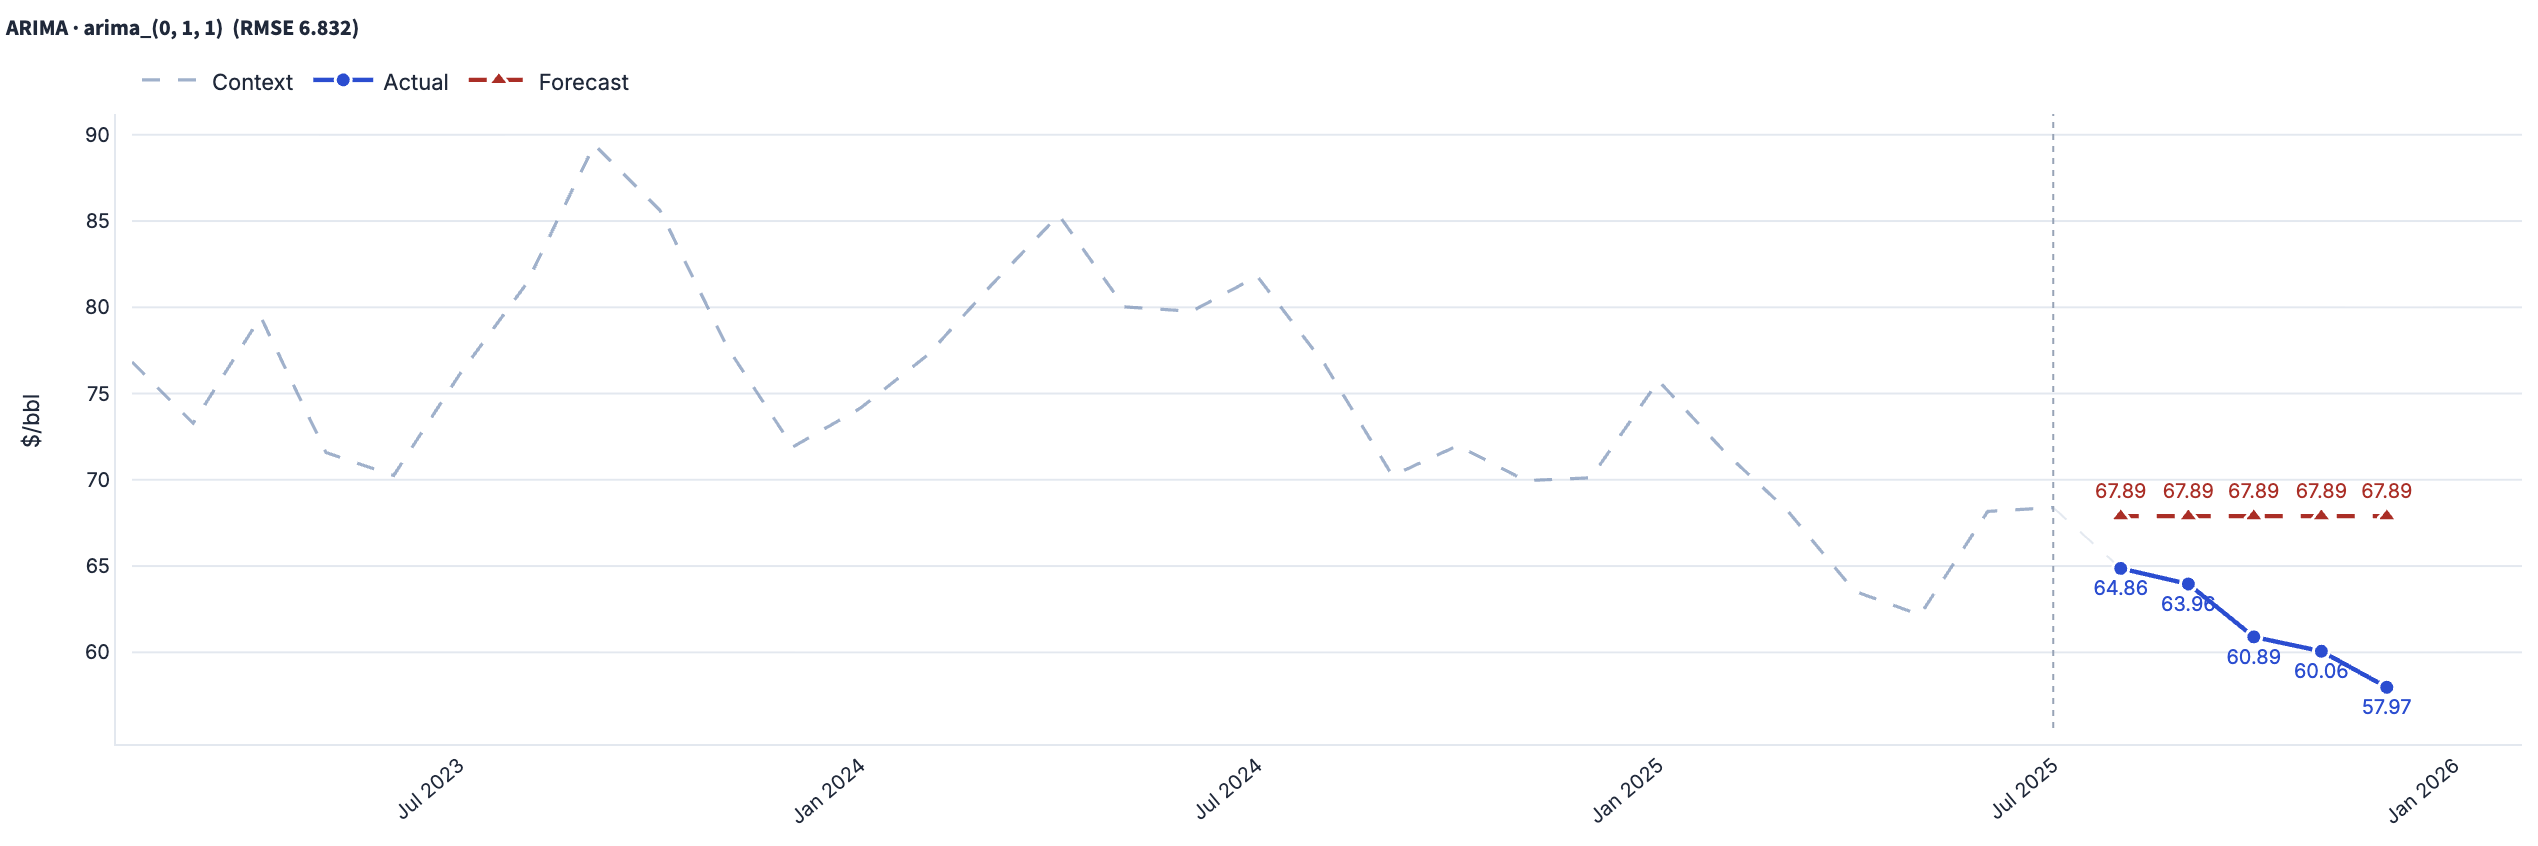
\includegraphics[width=\textwidth]{figures/univariate_arima_oil.png}
\small (a) ARIMA forecast for crude oil
\end{minipage}\hfill
\begin{minipage}[t]{0.48\textwidth}
\centering
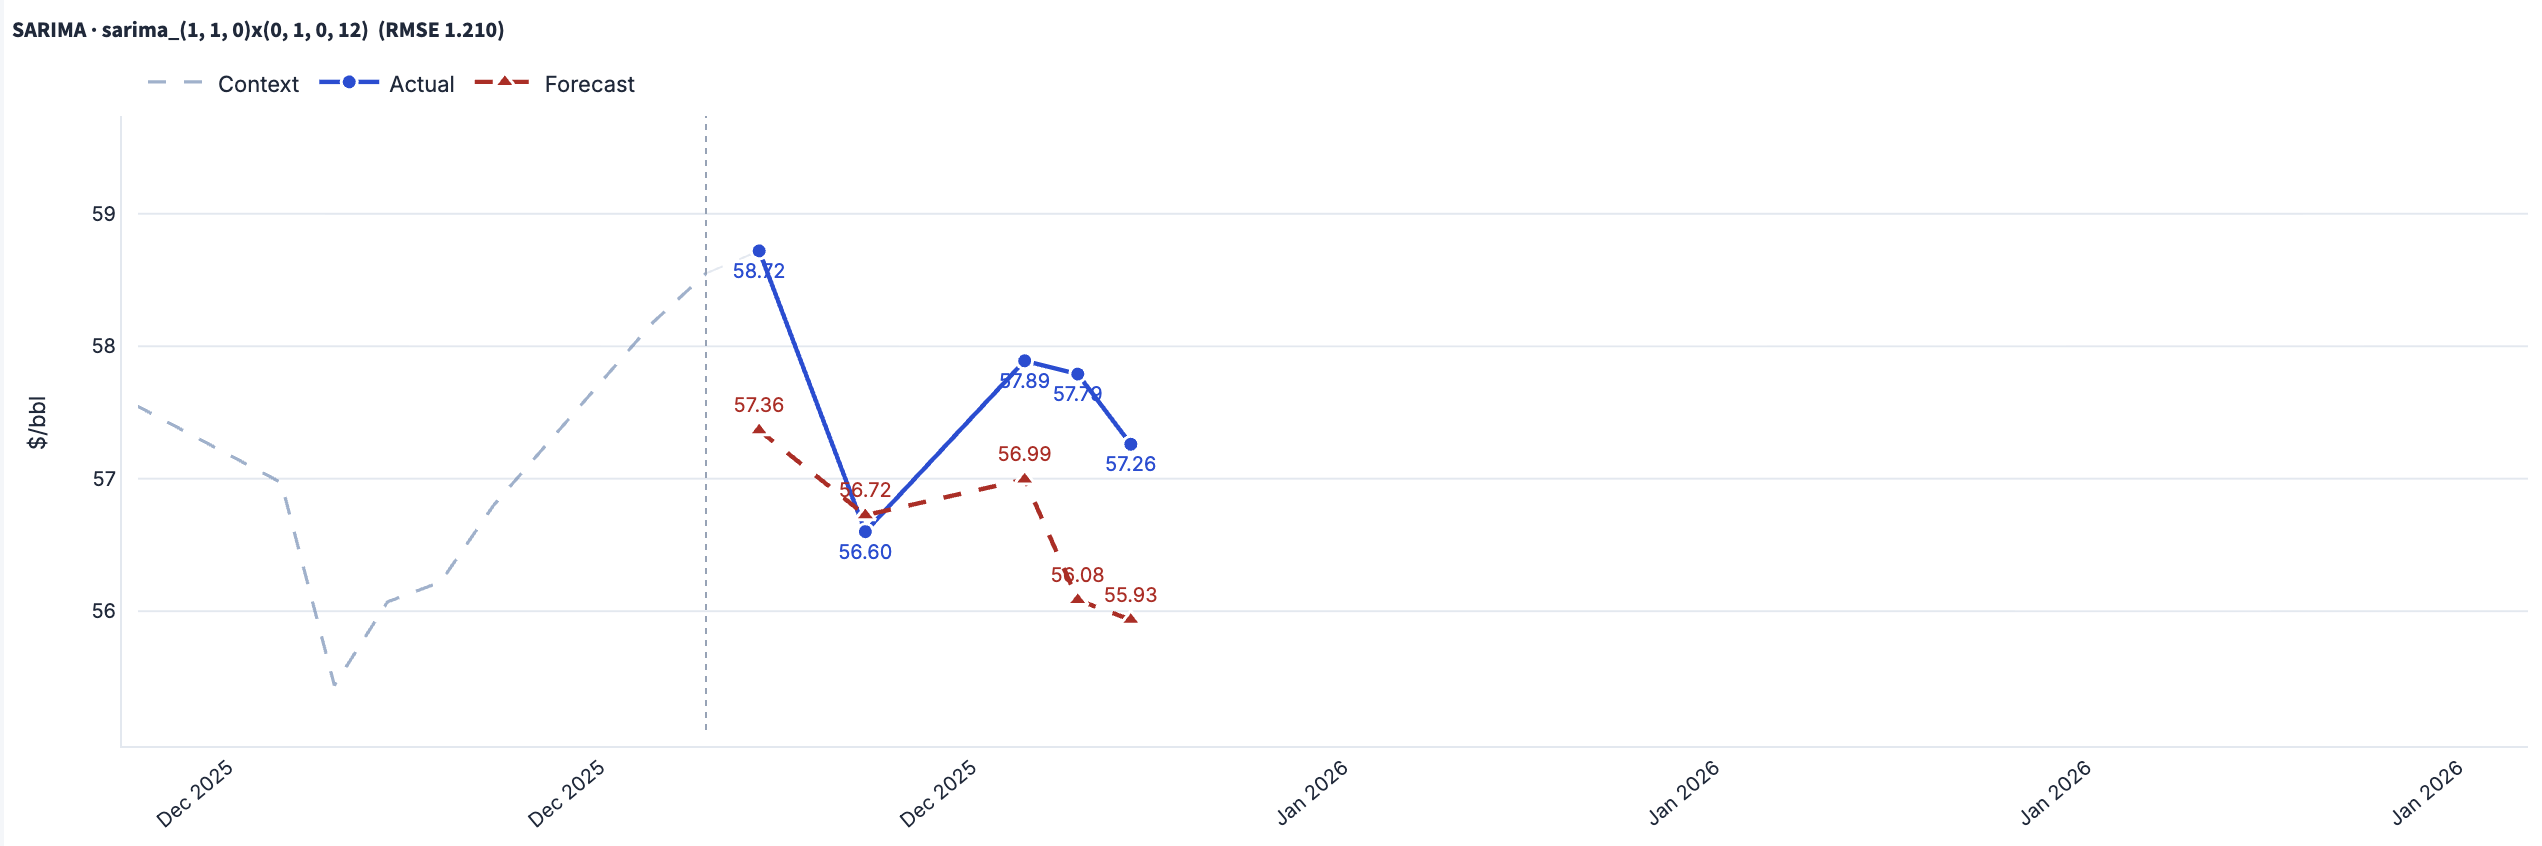
\includegraphics[width=\textwidth]{figures/univariate_sarima_oil.png}
\small (b) SARIMA forecast for crude oil
\end{minipage}

\vspace{0.5em}

\begin{minipage}[t]{0.48\textwidth}
\centering
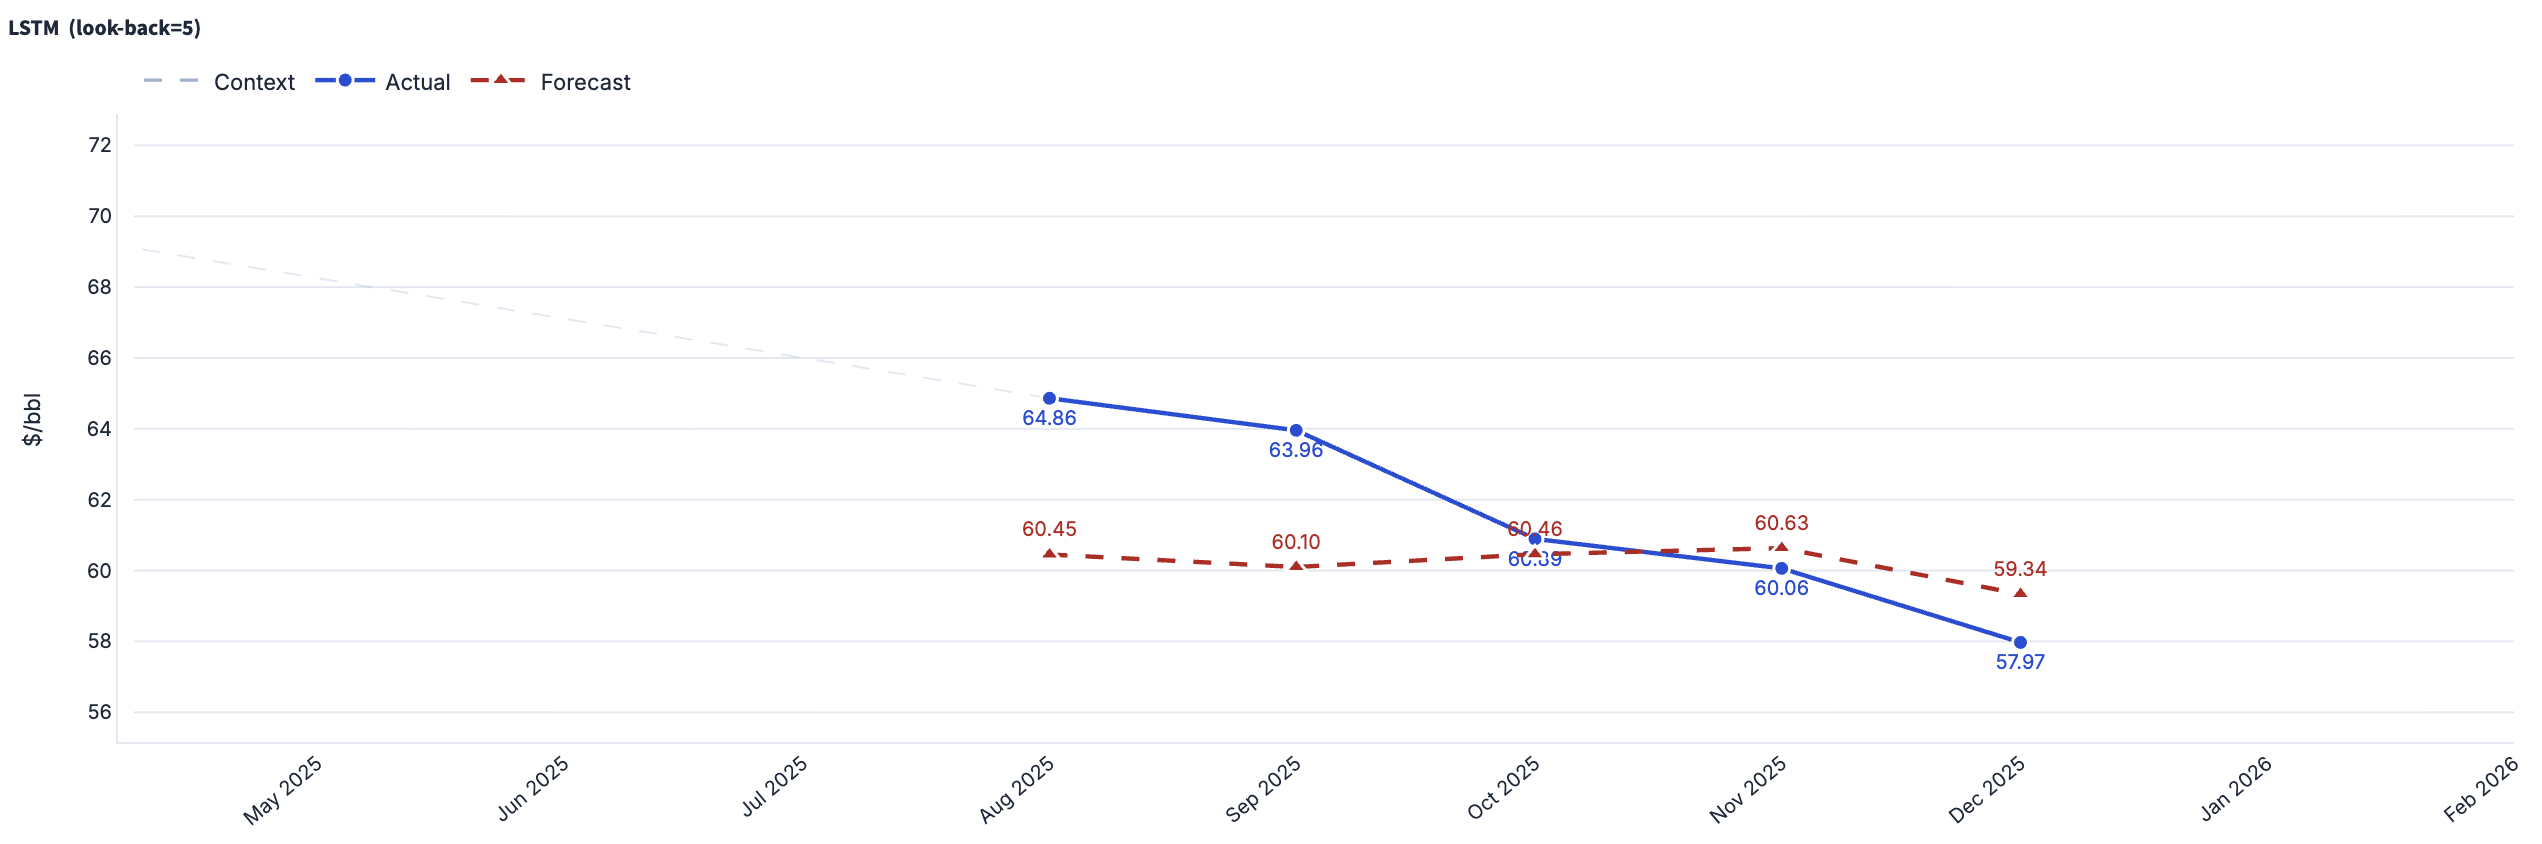
\includegraphics[width=\textwidth]{figures/univariate_oil_lstm_backtest.png}
\small (c) LSTM forecast for crude oil
\end{minipage}\hfill
\begin{minipage}[t]{0.48\textwidth}
\centering
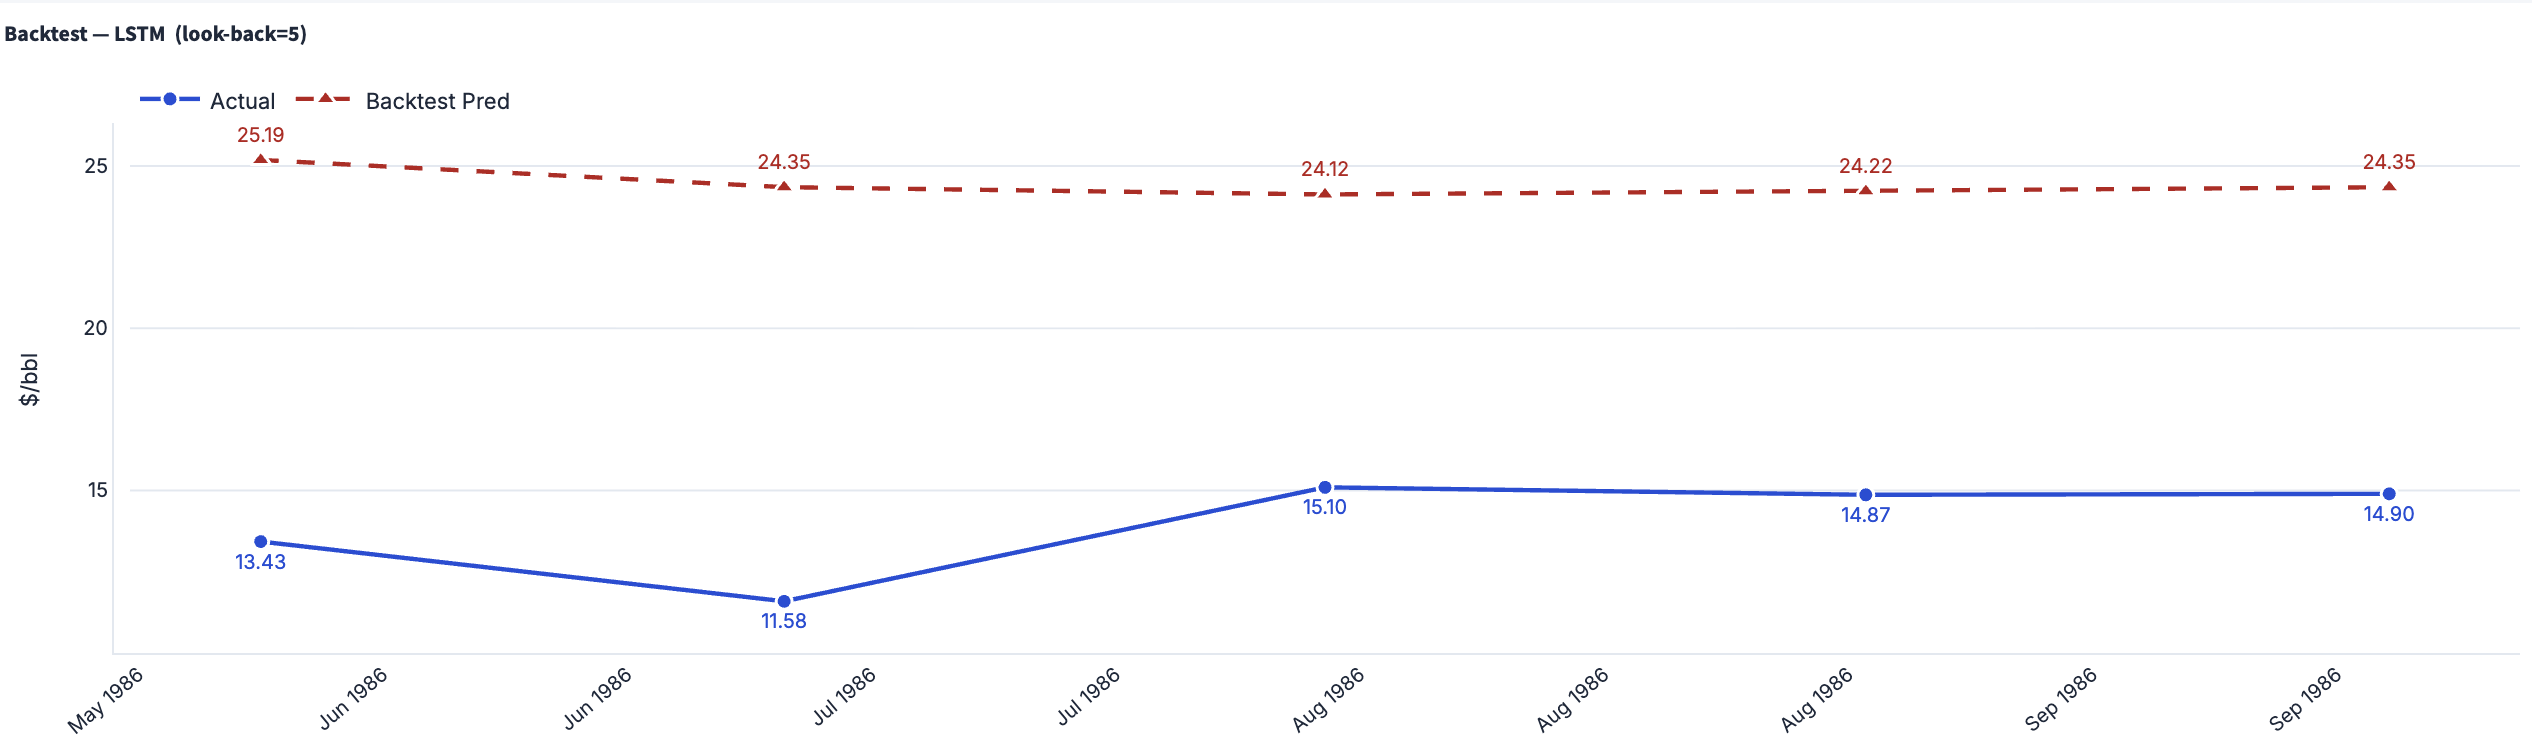
\includegraphics[width=\textwidth]{figures/univariate_oil_lstm.png}
\small (d) LSTM backtest for crude oil
\end{minipage}
\caption{Actual versus predicted WTI crude oil prices (USD/barrel, monthly, 2014--2024) across univariate model configurations: (a) ARIMA $(0,1,1)$, (b) SARIMA $(1,1,0) \times (0,1,0,12)$, (c) LSTM direct forecast, and (d) LSTM walk-forward backtest.}
\label{fig:univariate_crude_plots}
\end{figure}

\begin{table}[h]
\centering
\caption{Univariate model performance for crude oil}
\label{tab:univariate_crude}
\begin{tabular}{@{}lcccc@{}}
\toprule
Model & RMSE (USD/barrel) & MAE (USD/barrel) & MAPE (\%) & DA \\
\midrule
ARIMA & 6.832 & 6.343 & 10.49 & 0.20 \\
SARIMA & 1.210 & 1.081 & 1.87 & 0.60 \\
LSTM Forecast & 2.709 & 2.127 & -0.139 & 0.50 \\
LSTM Backtest & 10.578 & 10.471 & 76.78 & 0.10 \\
\botrule
\end{tabular}
\end{table}

As illustrated in Figure~\ref{fig:univariate_crude_plots}, the SARIMA model demonstrates the closest alignment with observed crude oil price dynamics, effectively tracking
seasonal cyclicality that the non-seasonal ARIMA specification and the LSTM model are unable to reproduce with comparable fidelity. In contrast, ARIMA produces smoother forecasts with limited responsiveness to fluctuations, while LSTM shows reasonable short-term tracking in the direct forecast setting but lacks consistency over time. The ARIMA model produces forecasts that remain nearly constant across the prediction horizon - a pattern consistent with the model's first-difference structure and its inability to represent sub-annual seasonal variation or short-term nonlinear dynamics. The SARIMA model improves this by incorporating seasonal structure, leading to forecasts that better follow the observed trend.

The LSTM forecasting plot shows smoother predictions that approximate the general level of the series but fail to respond to sharp changes. This suggests that the model does not adequately reproduce local variations. In the backtesting results, the LSTM predictions appear almost flat across rolling windows, while the actual series exhibits noticeable variability. This behavior leads to significantly higher RMSE and MAE values. The DA results reinforce this ranking: SARIMA reaches 0.60, outperforming ARIMA (0.20), LSTM forecast (0.50), and especially the LSTM backtest (0.10). Therefore, although backtesting is intended to verify temporal consistency, in this case it reveals that the model fails to represent non-trivial temporal dynamics and cannot be considered reliable for inference in the univariate setting. Overall, SARIMA performs better among the crude-oil univariate models in both error and directional terms.

The Diebold--Mariano results for crude oil support this interpretation. The ARIMA--SARIMA comparison is statistically significant ($\mathrm{DM}=-2.31$, $p=0.021$), confirming that the seasonal specification improves predictive accuracy relative to the non-seasonal baseline. By contrast, neither ARIMA versus LSTM ($p=0.064$) nor SARIMA versus LSTM ($p=0.150$) reaches the 5\% significance threshold, so the apparent ranking of LSTM relative to the classical models should be interpreted cautiously.

\begin{table}[h]
\centering
\small
\caption{Diebold--Mariano results for univariate crude oil models}
\begin{tabular}{@{}lrrrr@{}}
\toprule
Comparison & DM Stat & p-value & Significant \\
\midrule
ARIMA vs SARIMA & -2.31 & 0.021 & Yes \\
ARIMA vs LSTM & -1.85 & 0.064 & No \\
SARIMA vs LSTM & 1.42 & 0.150 & No \\
\botrule
\end{tabular}
\end{table}

\subsubsection*{5.1.2 Natural Gas (CNG)}\label{subsubsec:cngresults}

Table~\ref{tab:univariate_gas} and Figure~\ref{fig:univariate_gas_plots} summarize the natural-gas results by comparing the actual and predicted prices across ARIMA, SARIMA, and LSTM-based models.

\begin{figure}[h]
\centering
\begin{minipage}[t]{0.48\textwidth}
\centering
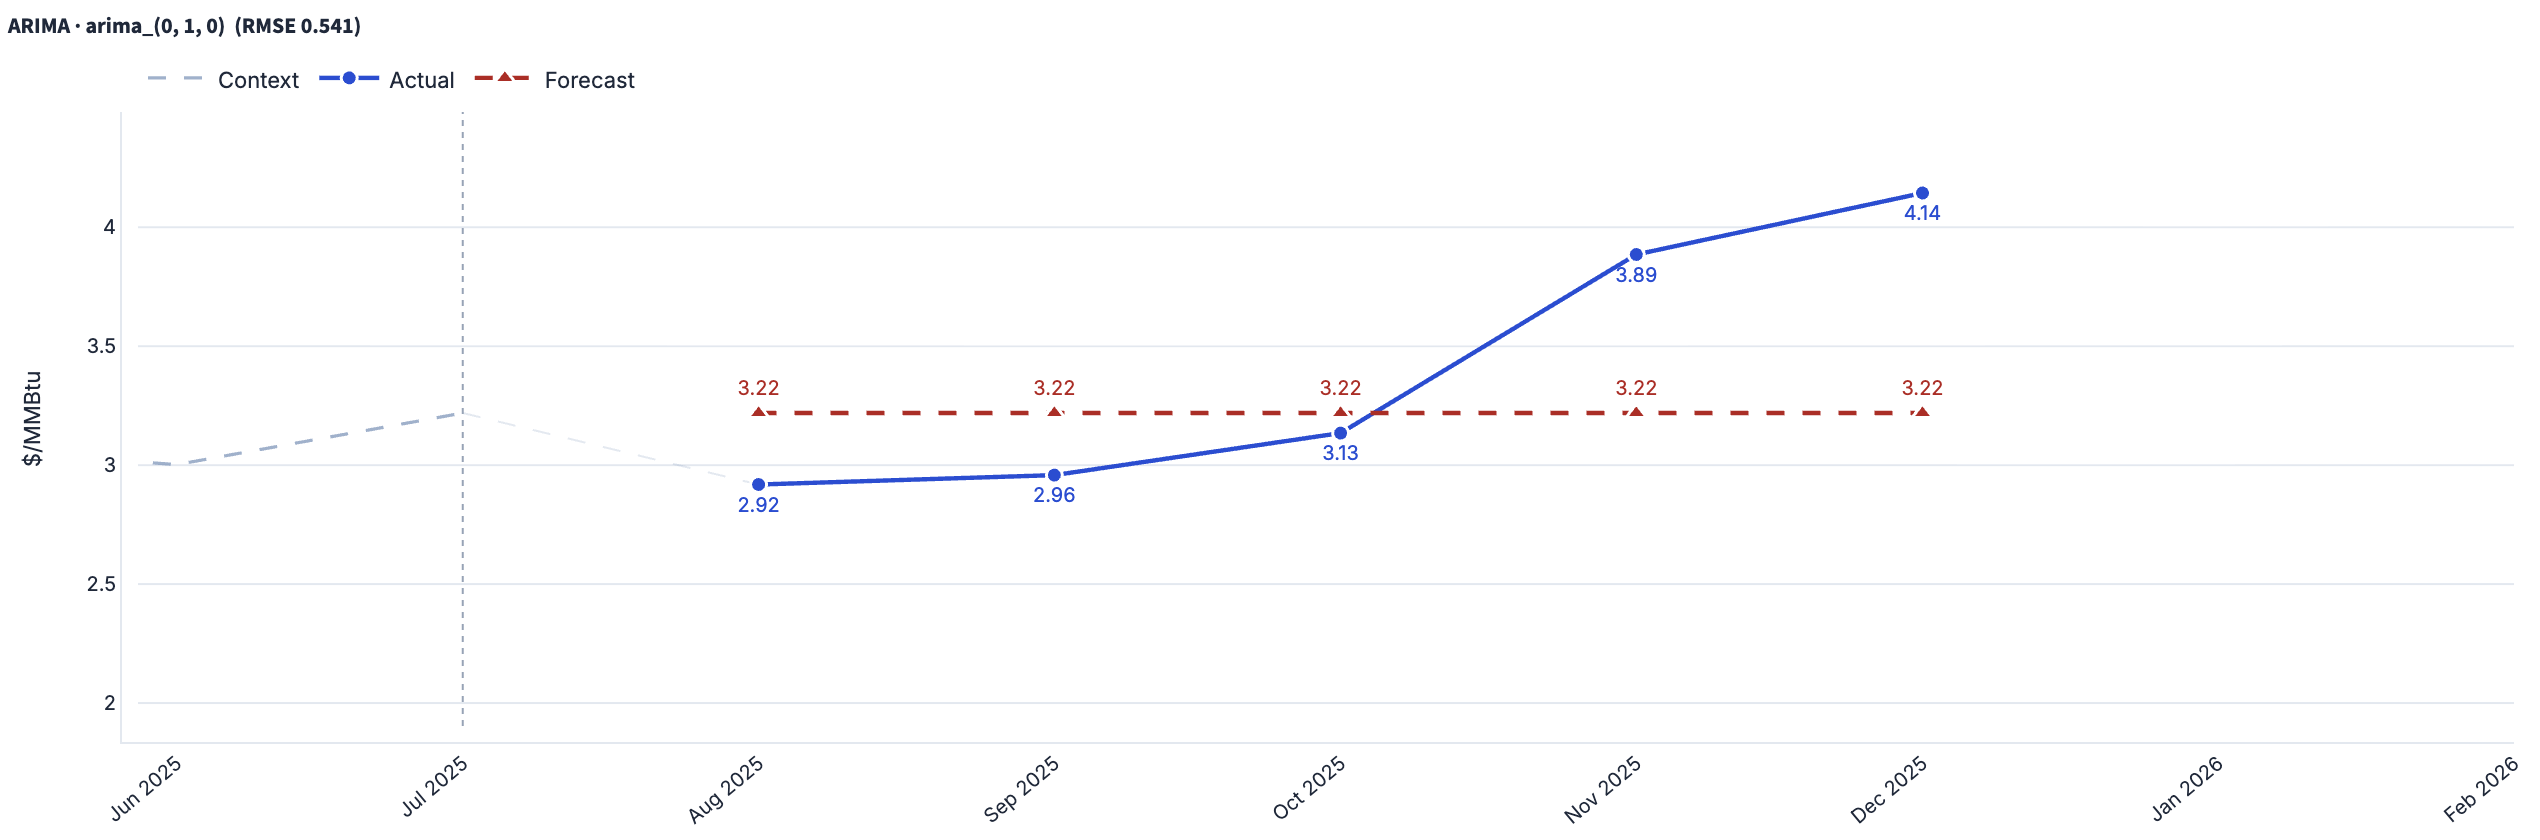
\includegraphics[width=\textwidth]{figures/univariate_arima_cng.png}
\small (a) ARIMA forecast for natural gas
\end{minipage}\hfill
\begin{minipage}[t]{0.48\textwidth}
\centering
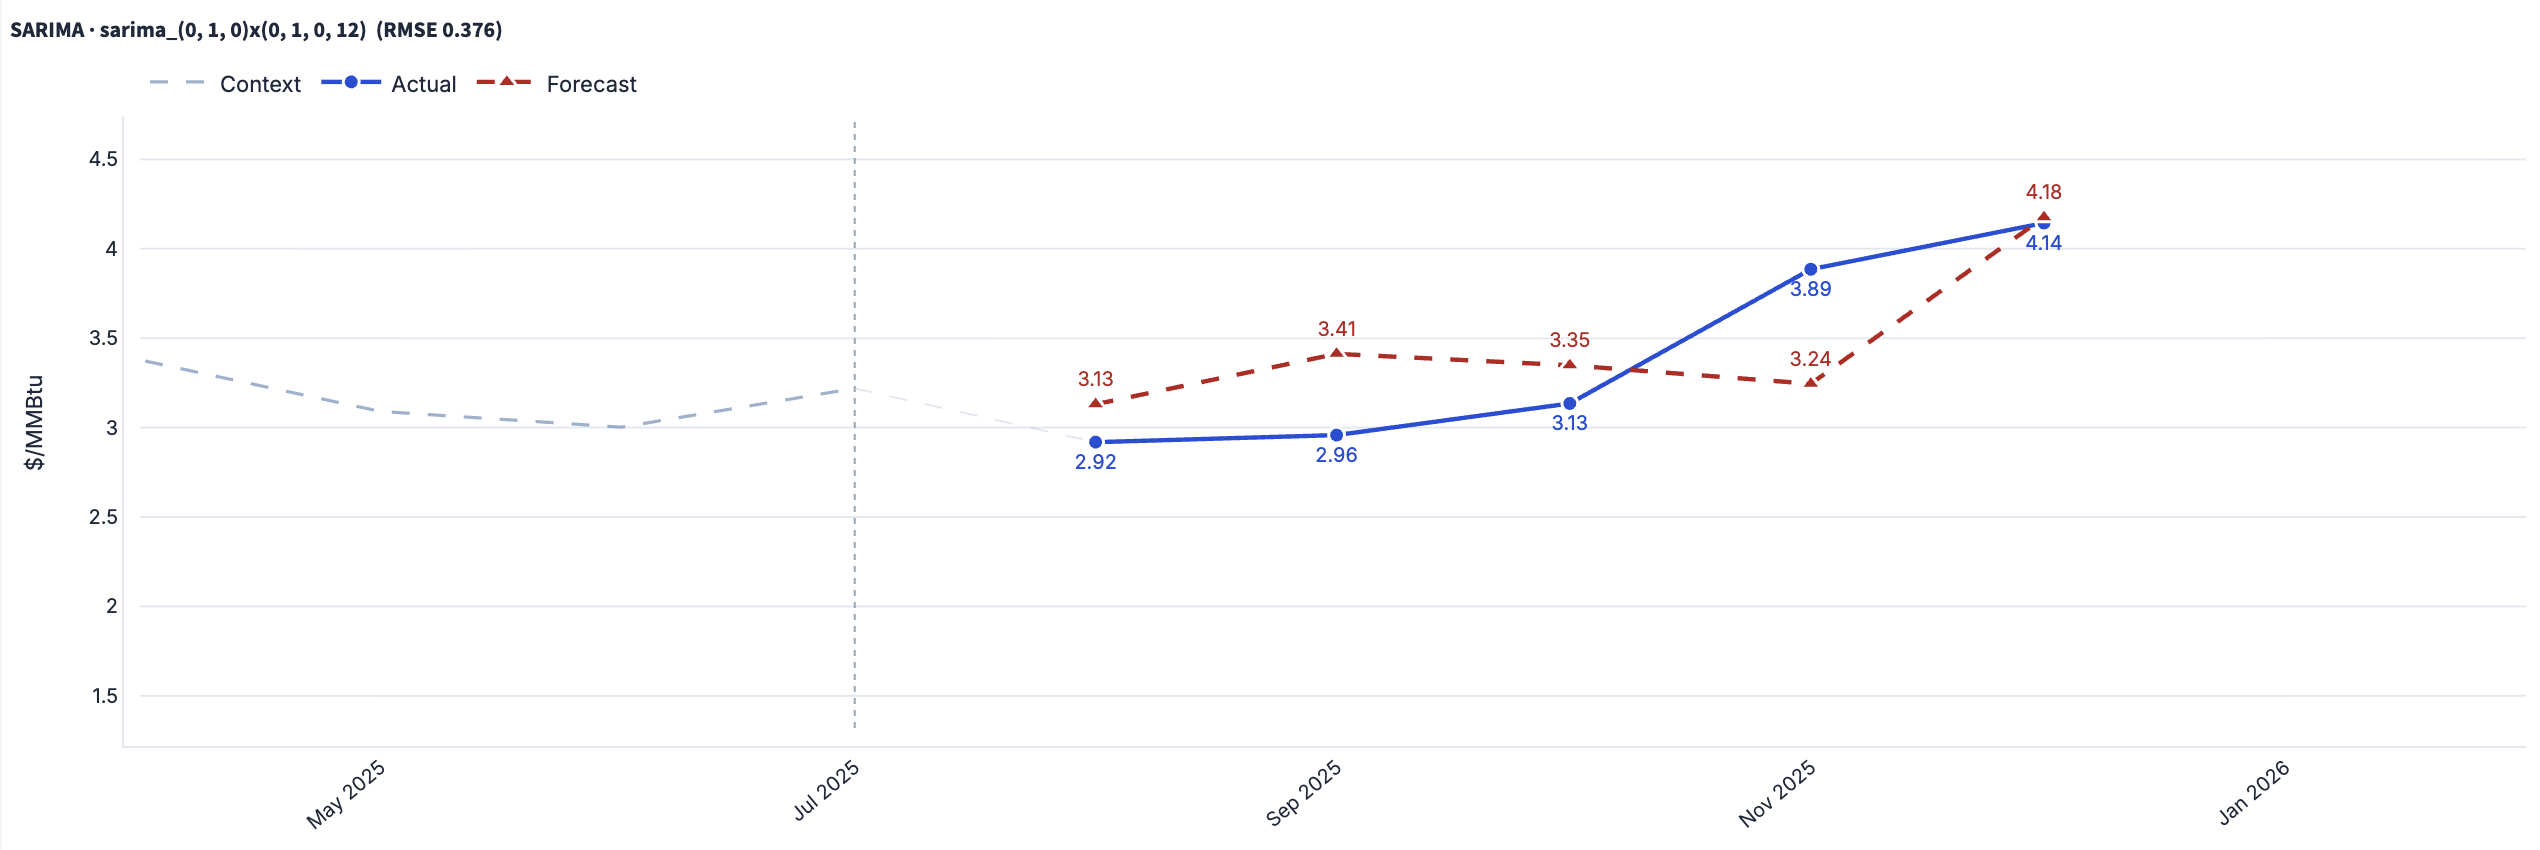
\includegraphics[width=\textwidth]{figures/univariate_sarima_cng.png}
\small (b) SARIMA forecast for natural gas
\end{minipage}

\vspace{0.5em}

\begin{minipage}[t]{0.48\textwidth}
\centering
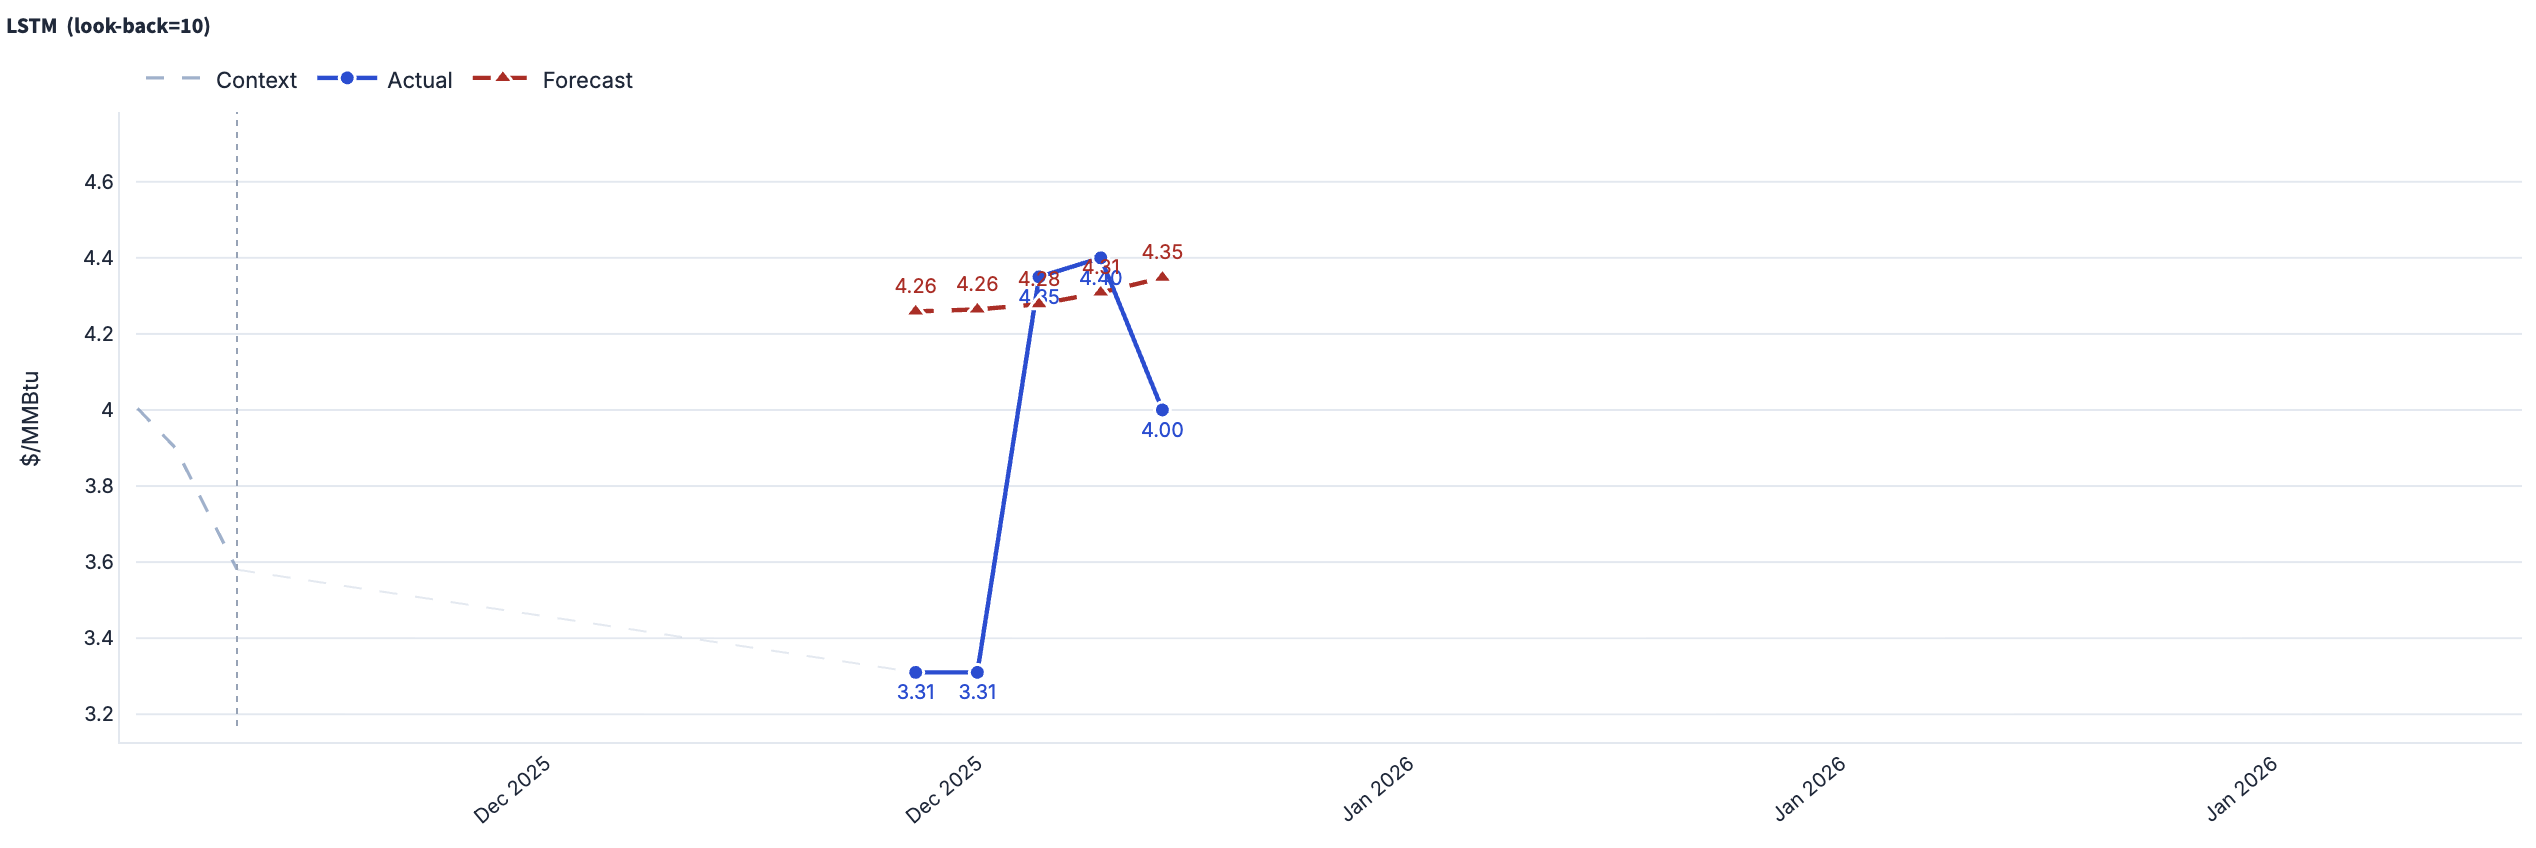
\includegraphics[width=\textwidth]{figures/univariate_cng_lstm.png}
\small (c) LSTM forecast for natural gas
\end{minipage}\hfill
\begin{minipage}[t]{0.48\textwidth}
\centering
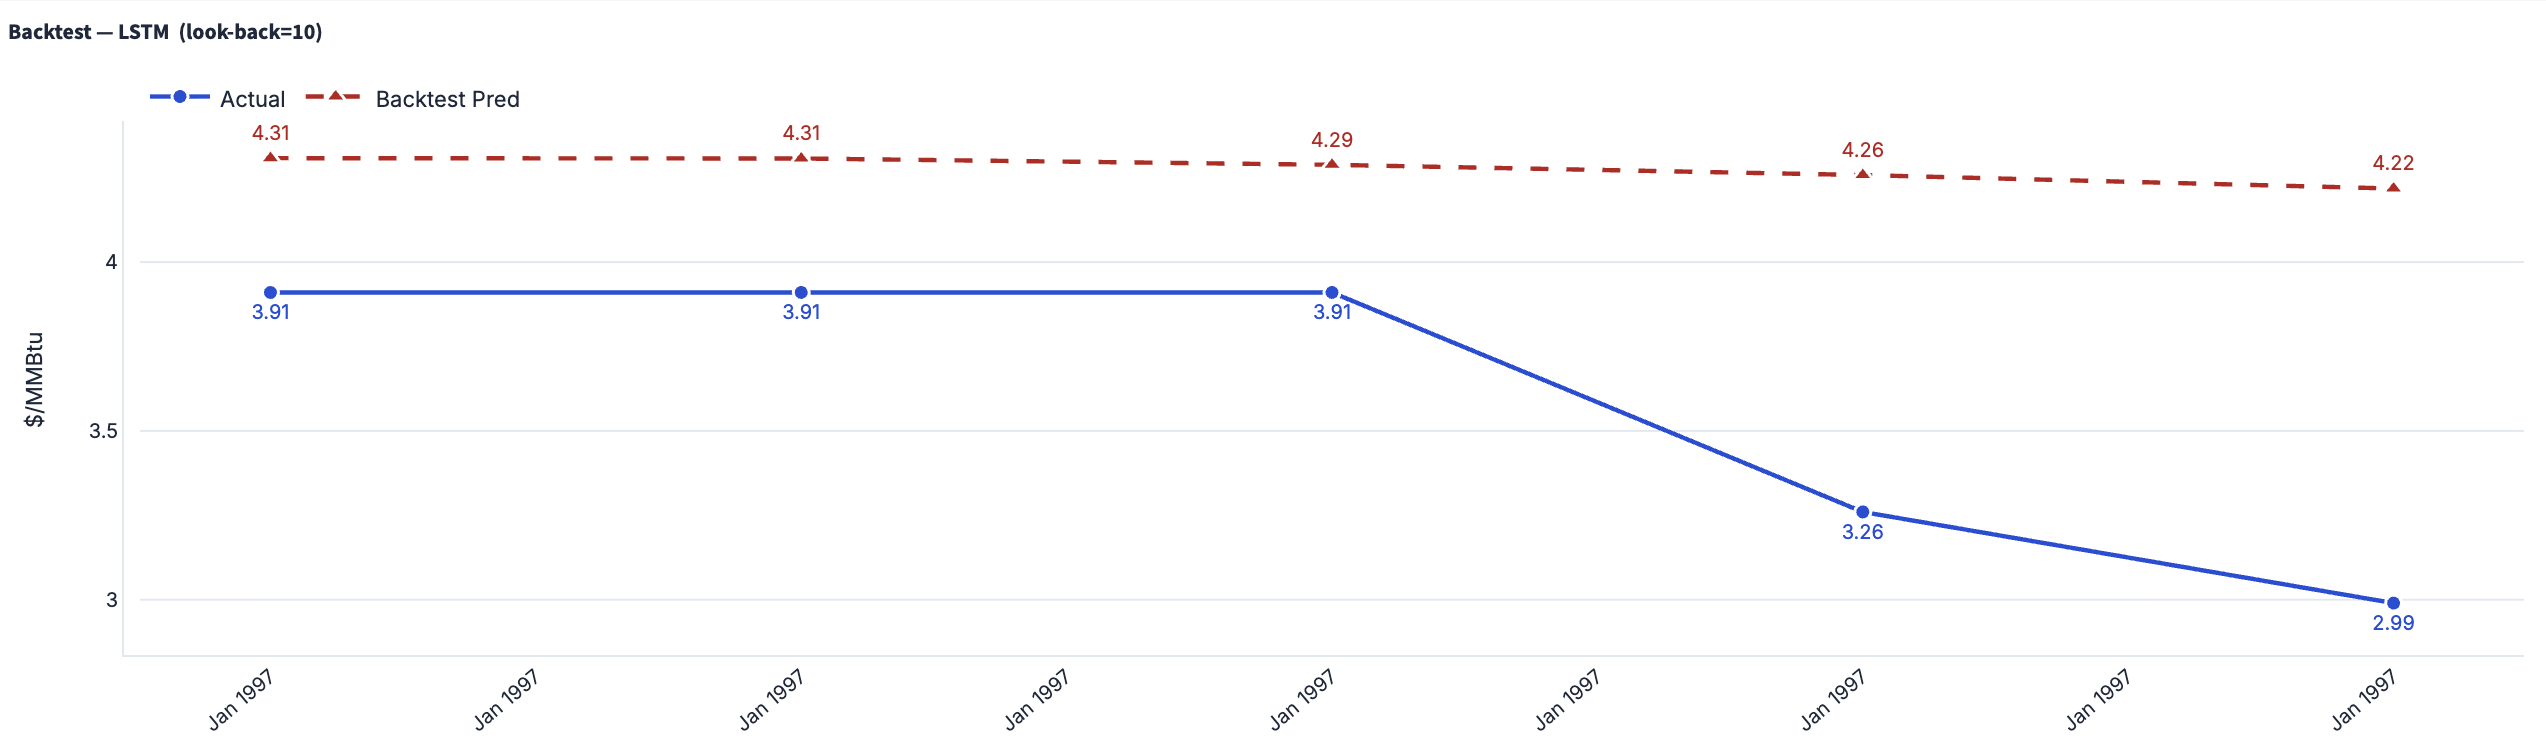
\includegraphics[width=\textwidth]{figures/univariate_cng_lstm_backtest.png}
\small (d) LSTM backtest for natural gas
\end{minipage}
\caption{Actual versus predicted Henry Hub natural gas prices (USD/MMBtu, monthly, 2014--2024) across univariate model configurations: (a) ARIMA $(0,1,0)$, (b) SARIMA $(0,1,0) \times (0,1,0,12)$, (c) LSTM direct forecast, and (d) LSTM walk-forward backtest.}
\label{fig:univariate_gas_plots}
\end{figure}

\begin{table}[h]
\centering
\caption{Univariate model performance for natural gas}
\label{tab:univariate_gas}
\begin{tabular}{@{}lcccc@{}}
\toprule
Model & RMSE (USD/MMBtu) & MAE (USD/MMBtu) & MAPE (\%) & DA \\
\midrule
ARIMA & 0.541 & 0.447 & 12.26 & 0.40 \\
SARIMA & 0.376 & 0.310 & 9.34 & 0.80 \\
LSTM Forecast & 0.624 & 0.483 & 13.99 & 0.60 \\
LSTM Backtest & 0.770 & 0.680 & 20.33 & 0.00 \\
\botrule
\end{tabular}
\end{table}

As shown in Figure~\ref{fig:univariate_gas_plots}, SARIMA again demonstrates superior performance by effectively tracking seasonal patterns in natural gas prices. ARIMA underfits the data, while LSTM exhibits moderate forecasting ability but reduced stability across time.

For natural gas (CNG), ARIMA again produces flat forecasts, while SARIMA better tracks the overall trend and seasonal movement. The LSTM forecasting results show noticeable deviation from actual values, indicating difficulty in modeling the series. In the  backtesting plots, predictions are relatively flat compared to the actual fluctuations, resulting in higher error. The DA values again favor SARIMA, which attains 0.80 versus 0.40 for ARIMA, 0.60 for the LSTM forecast, and 0.00 for the LSTM backtest. This suggests that the LSTM model does not generalize well across time and struggles to reproduce variability in the absence of additional explanatory features.

Overall, while SARIMA exhibits comparatively superior performance among the univariate model class, none of the approaches evaluated consistently reproduce the full range of variability and dynamic behavior exhibited by either energy price series - a finding that motivates the multivariate feature configurations examined in subsequent sections. These findings indicate that relying solely on historical price data is insufficient for robust forecasting, highlighting the need for incorporating additional explanatory variables to improve model performance.

The Diebold--Mariano test leads to a similar conclusion for natural gas. The only significant pairwise difference is again ARIMA versus SARIMA ($\mathrm{DM}=-2.05$, $p=0.040$), which reinforces the value of seasonal structure in the univariate setting. The comparisons involving LSTM are not statistically significant ($p=0.190$ for ARIMA versus LSTM and $p=0.370$ for SARIMA versus LSTM), indicating that its departures from the classical baselines are not stable enough to establish a clear predictive advantage.

\subsection{Multivariate Modelling}\label{subsec:multivariate_models}

This subsection presents the multivariate forecasting models developed by incorporating exogenous variables in addition to historical price data. The purpose of these models is to evaluate whether macroeconomic indicators, news-derived signals, or their combination improve forecasting performance beyond the univariate baselines. The models considered include SARIMAX, LSTM, and a hybrid CNN--LSTM architecture. To ensure robustness and reduce redundancy, multicollinearity among macroeconomic variables was assessed using the Variance Inflation Factor (VIF), as defined in Section~\ref{subsubsec:fredprocessing}, and variables with VIF greater than 8 were removed.

\subsubsection*{5.2.1 Macro Only}

In this setting, only macroeconomic variables were used as input features, excluding the target price series. To improve stability and reduce redundancy, multicollinearity among the macroeconomic variables was evaluated using the Variance Inflation Factor (VIF), and variables with VIF greater than 8 were removed before model fitting. The models evaluated in this setting were SARIMAX, LSTM, and CNN--LSTM. For the neural models, both LSTM and CNN--LSTM were trained using an input window of 36 time steps and a single-step output.

\subsubsection*{5.2.1.1 Crude Oil}
For crude oil, we evaluated SARIMAX, LSTM, and CNN--LSTM models using macroeconomic features. Table~\ref{tab:macro_only_oil} summarizes the performance results, and Figure~\ref{fig:macro_only_oil_plots} shows the corresponding predictions.

\begin{figure}[h]
\centering
\begin{minipage}[t]{0.48\textwidth}
\centering
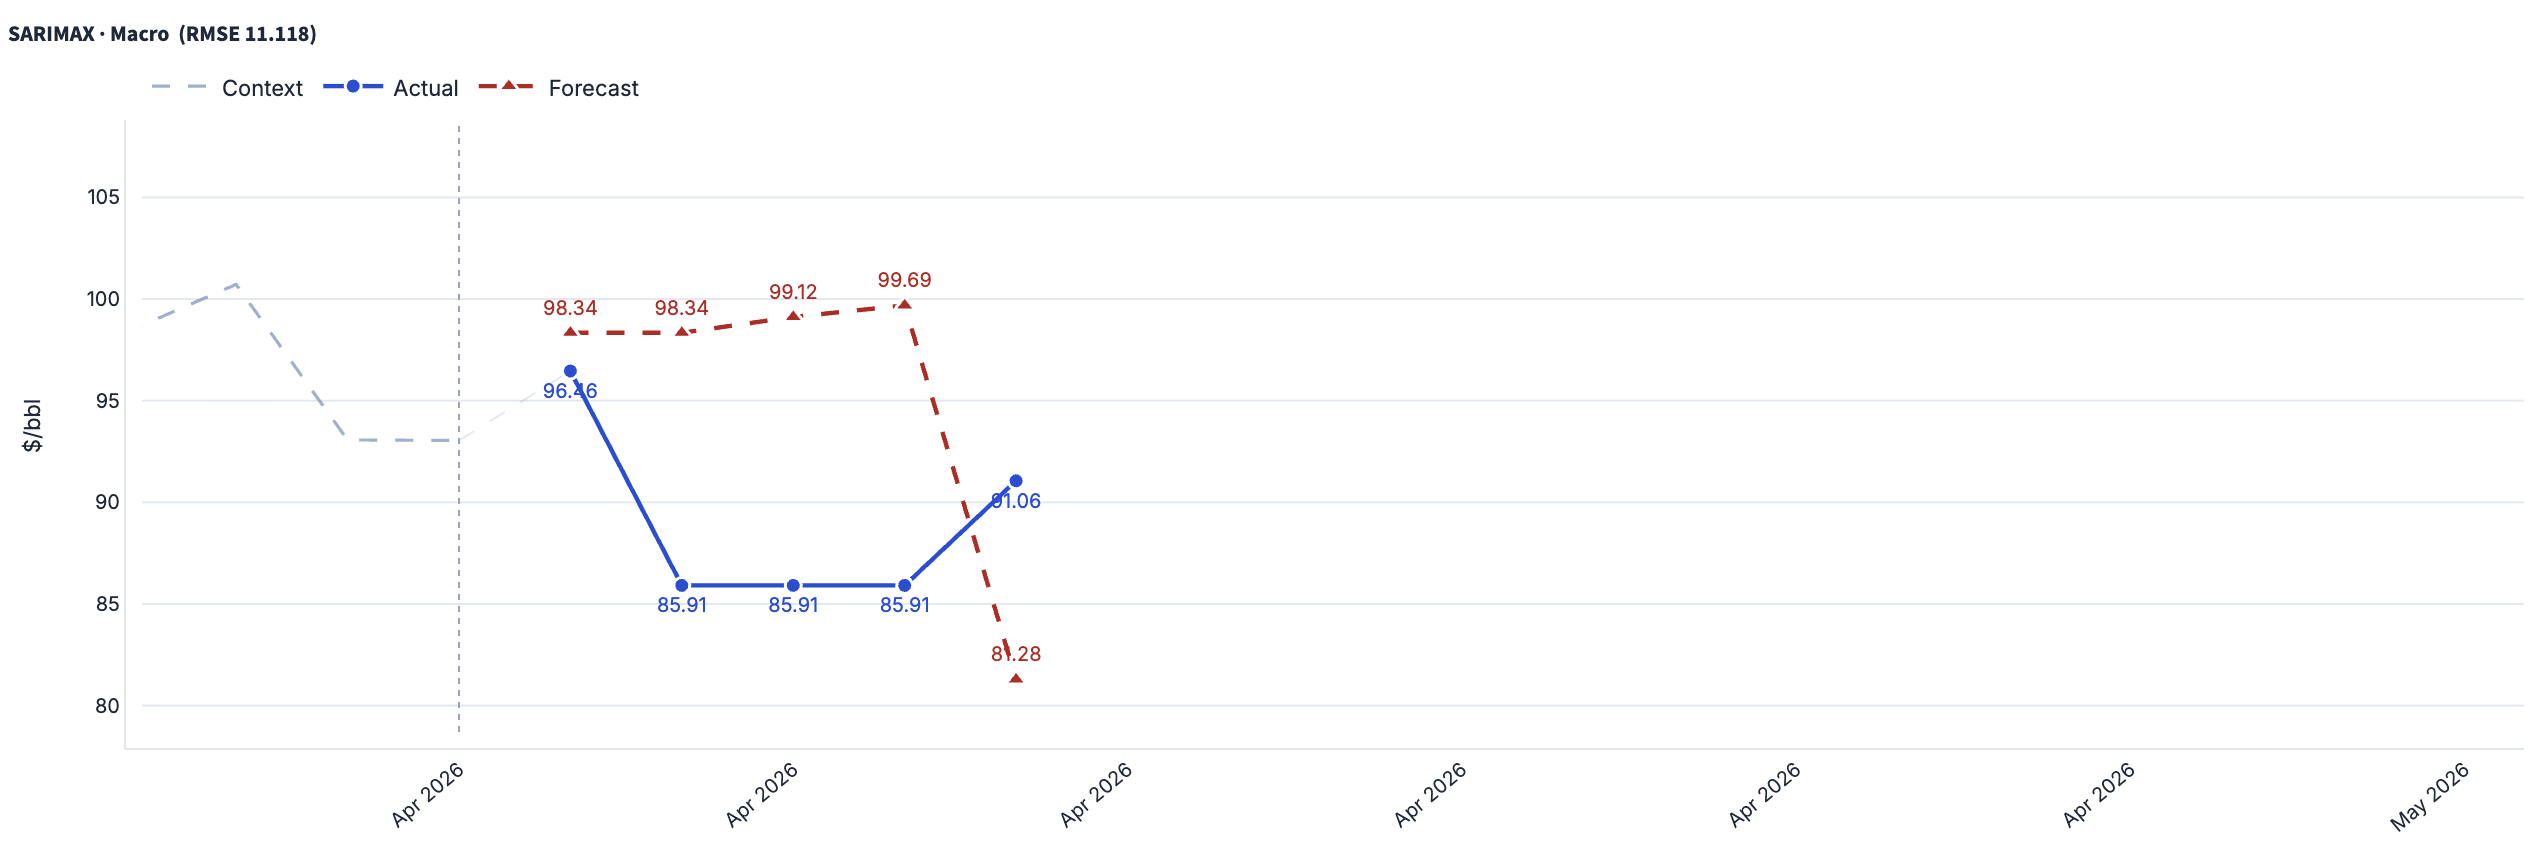
\includegraphics[width=\textwidth]{figures/multivariate_macro_oil_sarimax.png}
\small (a) SARIMAX forecast for crude oil
\end{minipage}\hfill
\begin{minipage}[t]{0.48\textwidth}
\centering
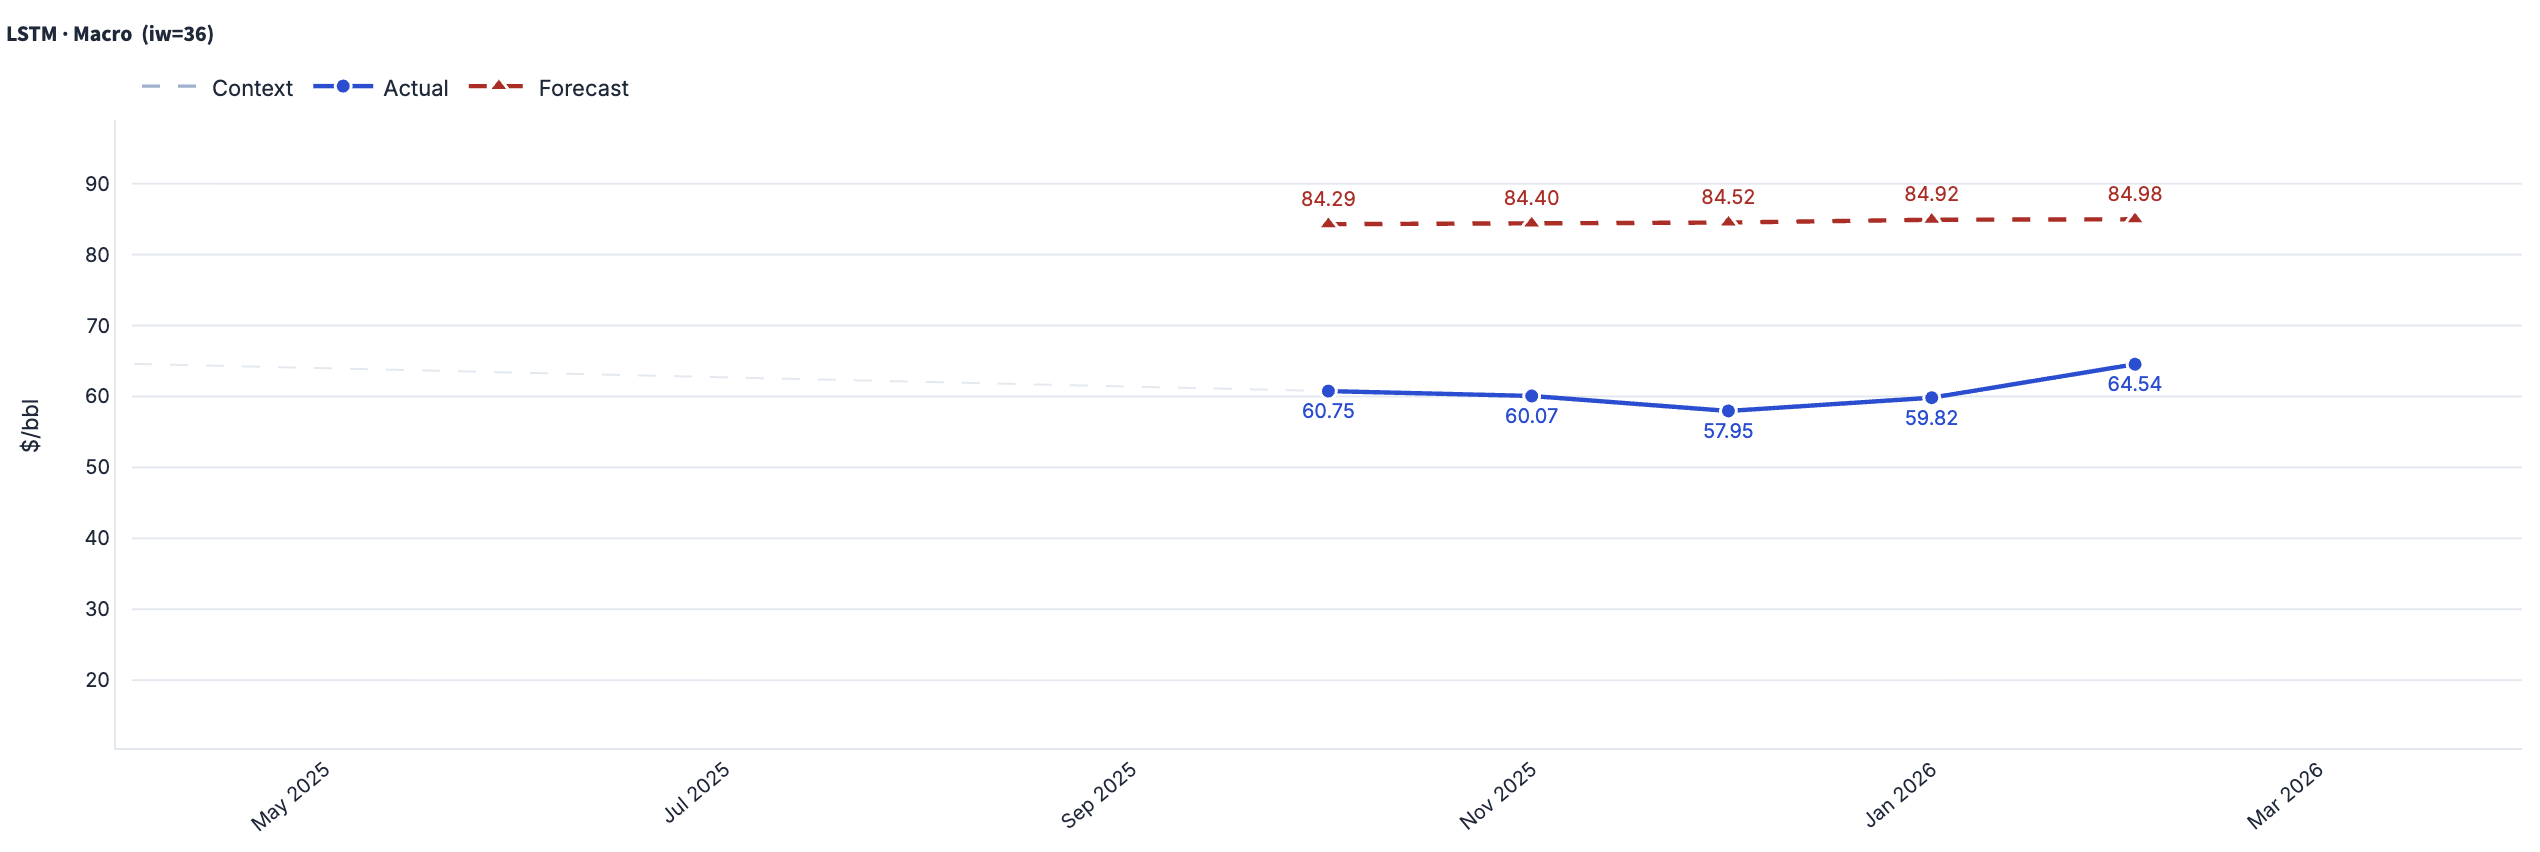
\includegraphics[width=\textwidth]{figures/multivaiate_macro_oil_lstm.png}
\small (b) LSTM forecast for crude oil
\end{minipage}

\vspace{0.5em}

\begin{minipage}[t]{0.48\textwidth}
\centering
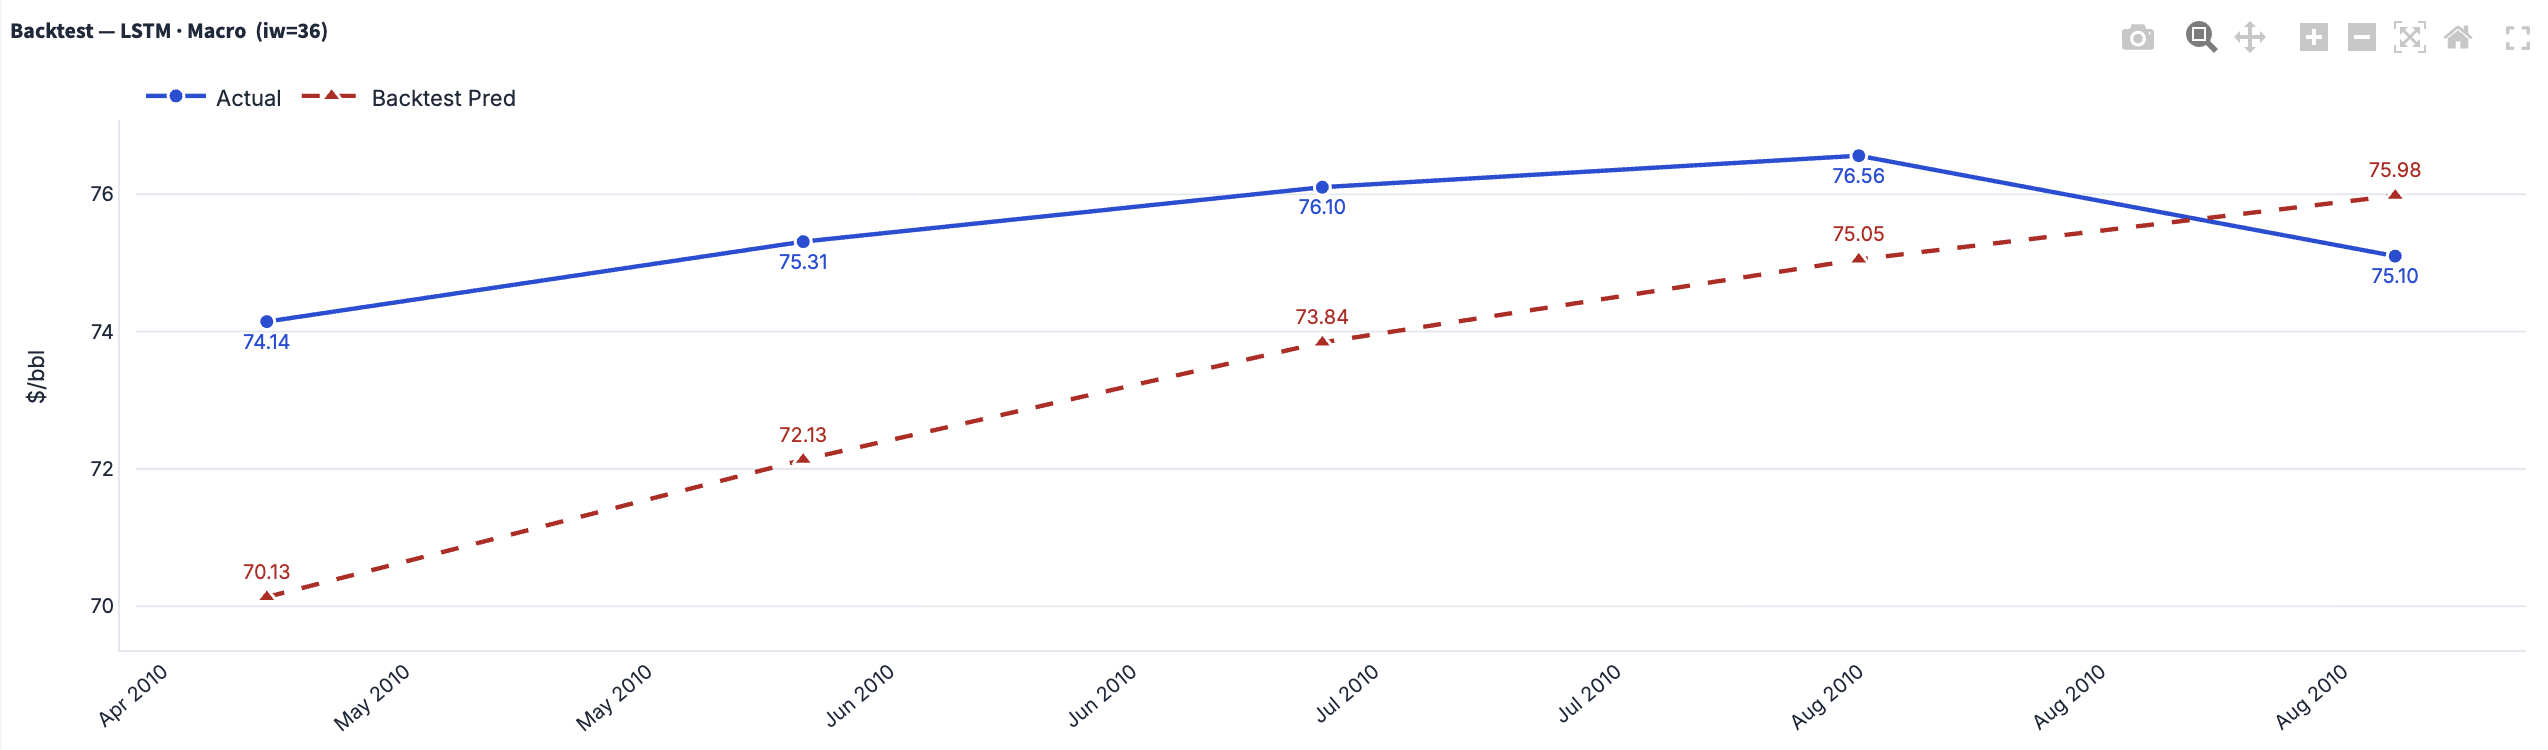
\includegraphics[width=\textwidth]{figures/multivariate_macro_oil_lstm_backtest.png}
\small (c) LSTM backtest for crude oil
\end{minipage}\hfill
\begin{minipage}[t]{0.48\textwidth}
\centering
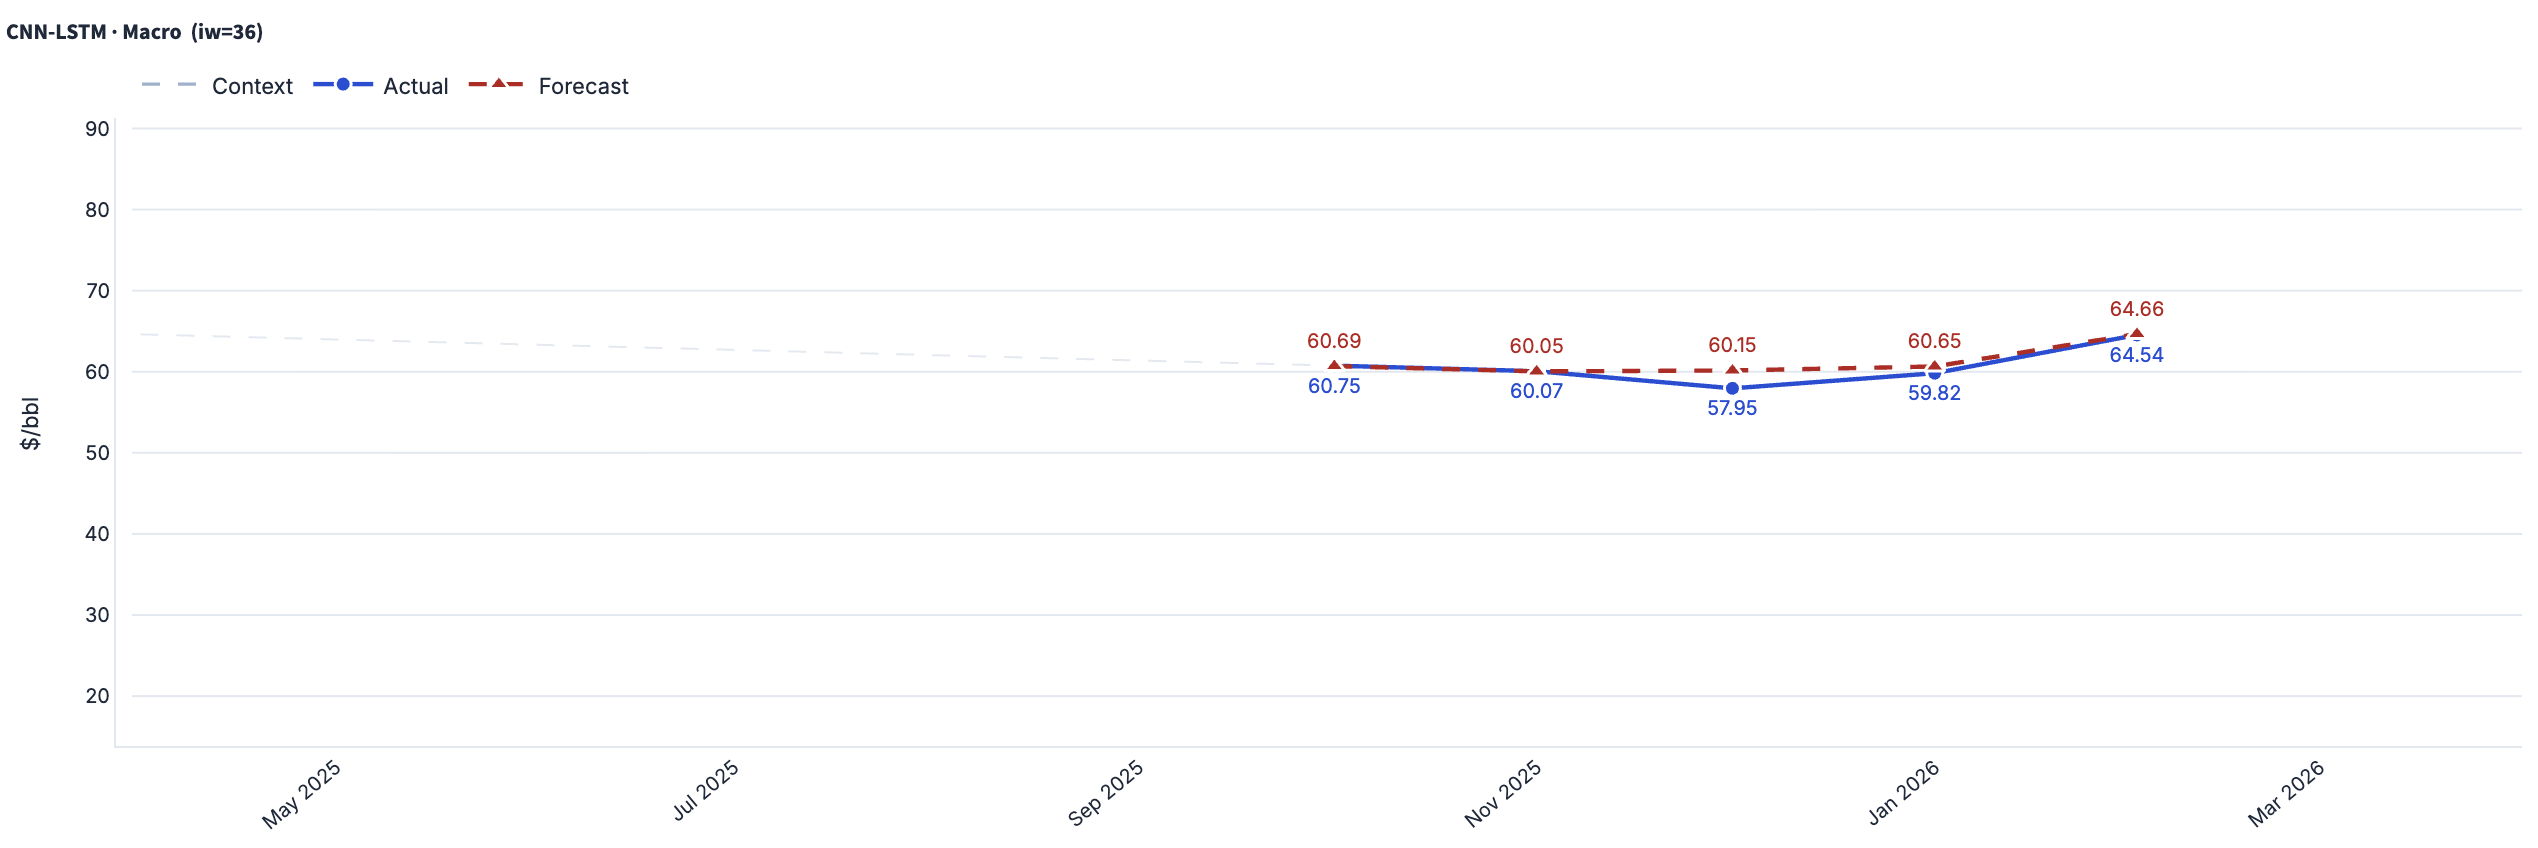
\includegraphics[width=\textwidth]{figures/multivariate_macro_oil_cnnlstm.png}
\small (d) CNN--LSTM forecast for crude oil
\end{minipage}

\vspace{0.5em}

\begin{minipage}[t]{0.48\textwidth}
\centering
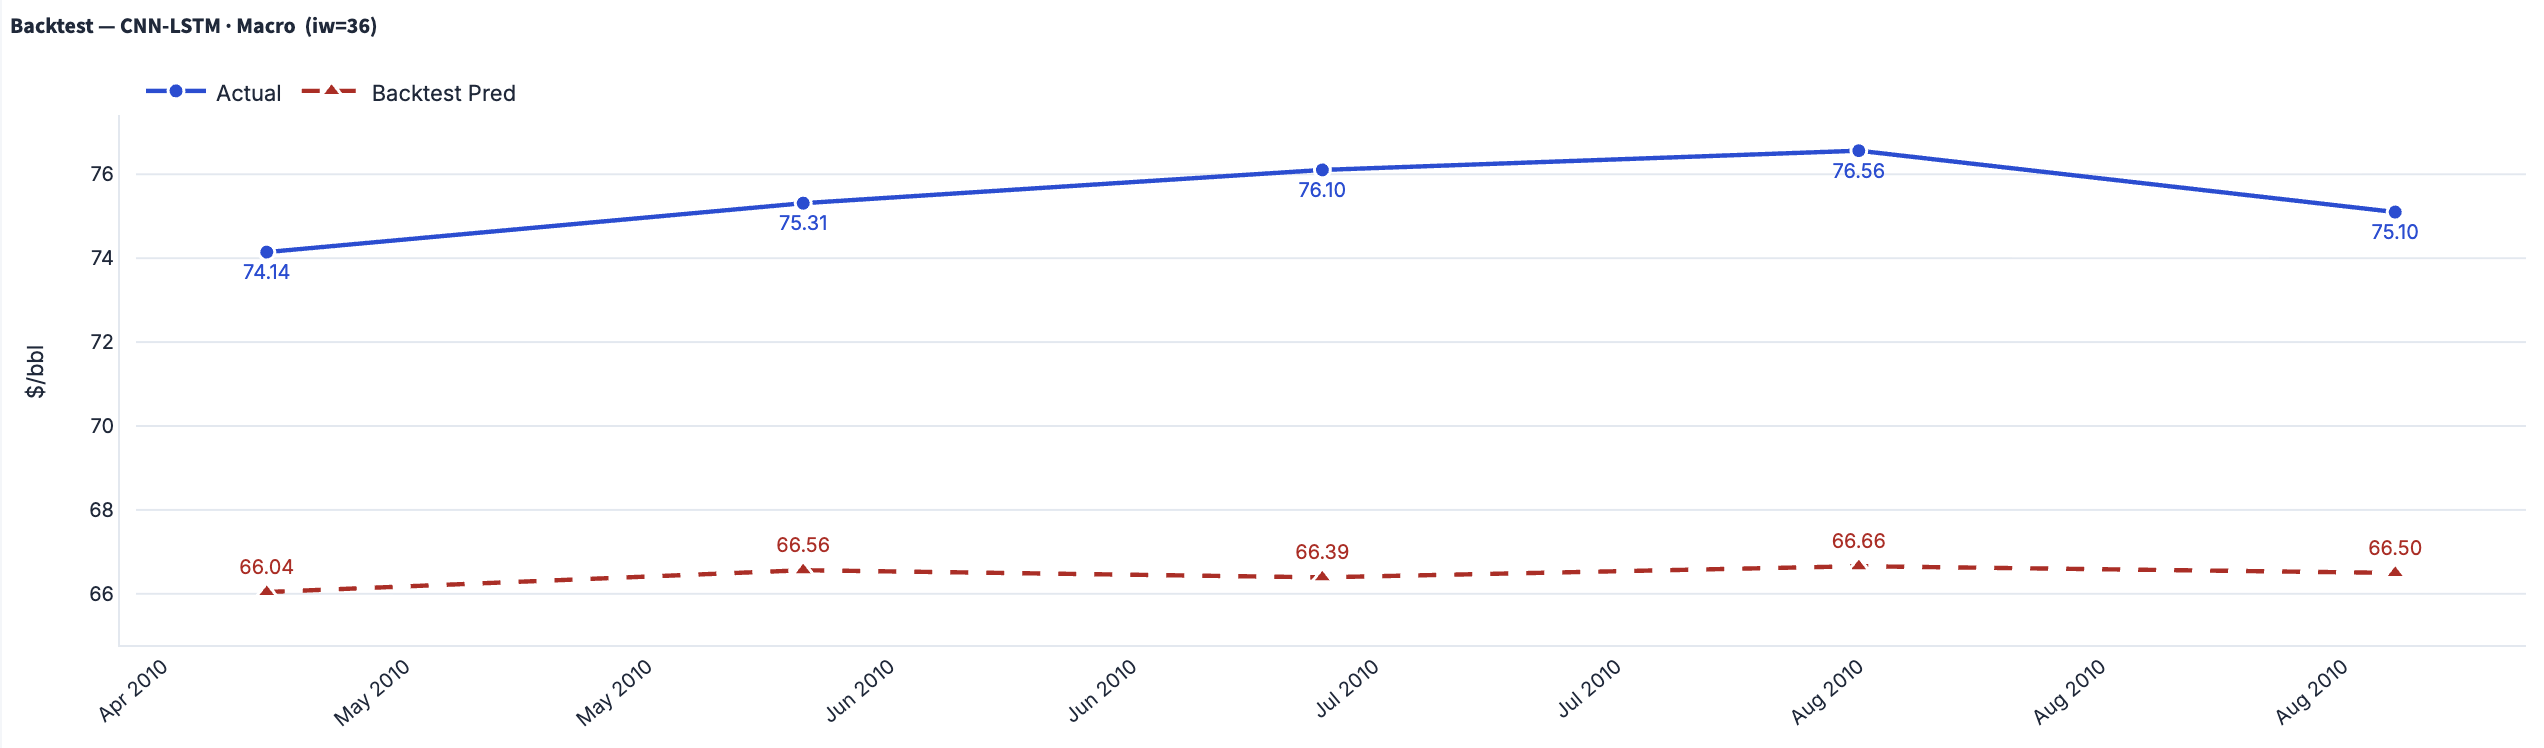
\includegraphics[width=\textwidth]{figures/multivariate_macro_oil_cnnlstm_backtest.png}
\small (e) CNN--LSTM backtest for crude oil
\end{minipage}
\caption{Actual versus predicted WTI crude oil prices (USD/barrel) using macroeconomic variables only: (a) SARIMAX forecast with exogenous FRED indicators, (b) LSTM direct forecast, (c) LSTM walk-forward backtest, (d) CNN--LSTM direct forecast, and (e) CNN--LSTM walk-forward backtest. This figure summarizes the macro-only multivariate setting.}
\label{fig:macro_only_oil_plots}
\end{figure}

\begin{table}[h]
\centering
\caption{Macro-only multivariate model performance for crude oil}
\label{tab:macro_only_oil}
\begin{tabular}{@{}lcccc@{}}
\toprule
Model & RMSE (USD/barrel) & MAE (USD/barrel) & MAPE (\%) & DA \\
\midrule
SARIMAX & 24.081 & 23.995 & 39.74 & 0.40 \\
LSTM Forecast & 24.081 & 23.995 & 39.74 & 0.20 \\
LSTM Backtest & 2.621 & 2.368 & 3.15 & 0.75 \\
CNN--LSTM Forecast & 1.054 & 0.647 & 1.10 & 0.80 \\
CNN--LSTM Backtest & 9.038 & 9.012 & 11.94 & 0.00 \\
\botrule
\end{tabular}
\end{table}

Figure~\ref{fig:macro_only_oil_plots} shows that SARIMAX and LSTM struggle to recover the movement of crude oil prices when only macroeconomic variables are used. Their forecasts remain either too smooth or poorly aligned with the observed series, which is reflected in the large forecast errors reported in Table~\ref{tab:macro_only_oil}. These results suggest that the direct linear relationship between the selected macroeconomic indicators and short-term crude oil price movements is weak in this setting.

By contrast, the CNN--LSTM forecast achieves the lowest forecast error among the macro-only crude-oil models and the highest DA (0.80), indicating that the hybrid architecture is better able to extract short-term temporal structure from the macroeconomic inputs. However, this gain does not fully carry over to backtesting: the CNN--LSTM backtest DA falls to 0.00 even though the LSTM backtest attains 0.75 with a markedly higher RMSE than the CNN--LSTM forecast. A similar inconsistency is visible for LSTM, whose backtest performance is much stronger than its direct forecast performance. Taken together, these results indicate that macroeconomic variables alone do not provide a stable or sufficiently informative basis for accurate crude-oil forecasting, even when more flexible neural architectures are used.

The DM comparisons sharpen this interpretation. For crude oil under the macro-only setting, CNN--LSTM significantly outperforms SARIMAX ($\mathrm{DM}=-2.75$, $p=0.006$) and also significantly outperforms LSTM ($\mathrm{DM}=-2.10$, $p=0.035$). The SARIMAX--LSTM comparison is only borderline ($\mathrm{DM}=-1.95$, $p=0.051$), so the clearest statistical result in this subsection is that CNN--LSTM yields the most defensible forecast improvement among the macro-only crude-oil models.

\subsubsection*{5.2.1.2 Natural Gas (CNG)}
For natural gas, Table~\ref{tab:macro_only_cng} summarizes the macro-only model results, and Figure~\ref{fig:macro_only_cng_plots} shows the corresponding prediction plots.

\begin{figure}[h]
\centering
\begin{minipage}[t]{0.48\textwidth}
\centering
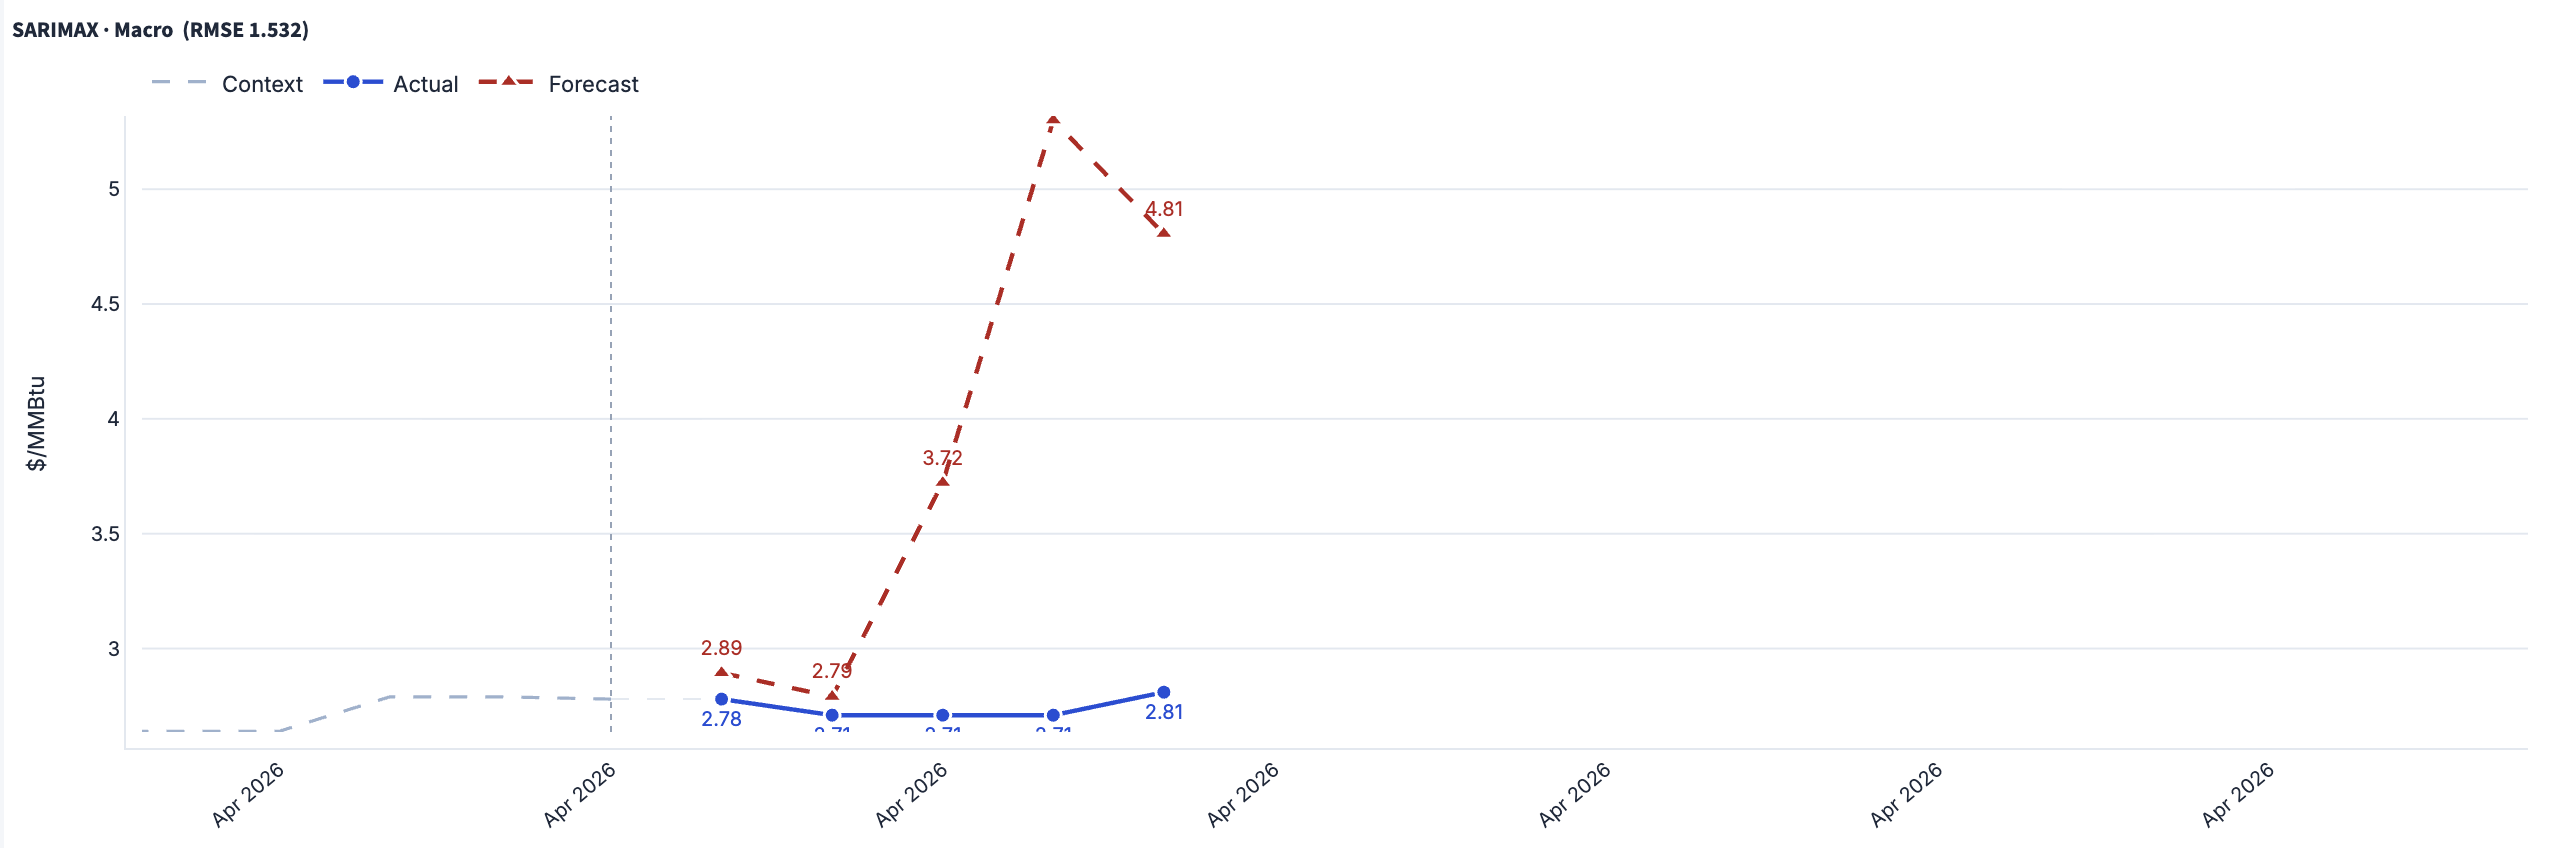
\includegraphics[width=\textwidth]{figures/multivariate_macro_cng_sarimax.png}
\small (a) SARIMAX forecast for natural gas
\end{minipage}\hfill
\begin{minipage}[t]{0.48\textwidth}
\centering
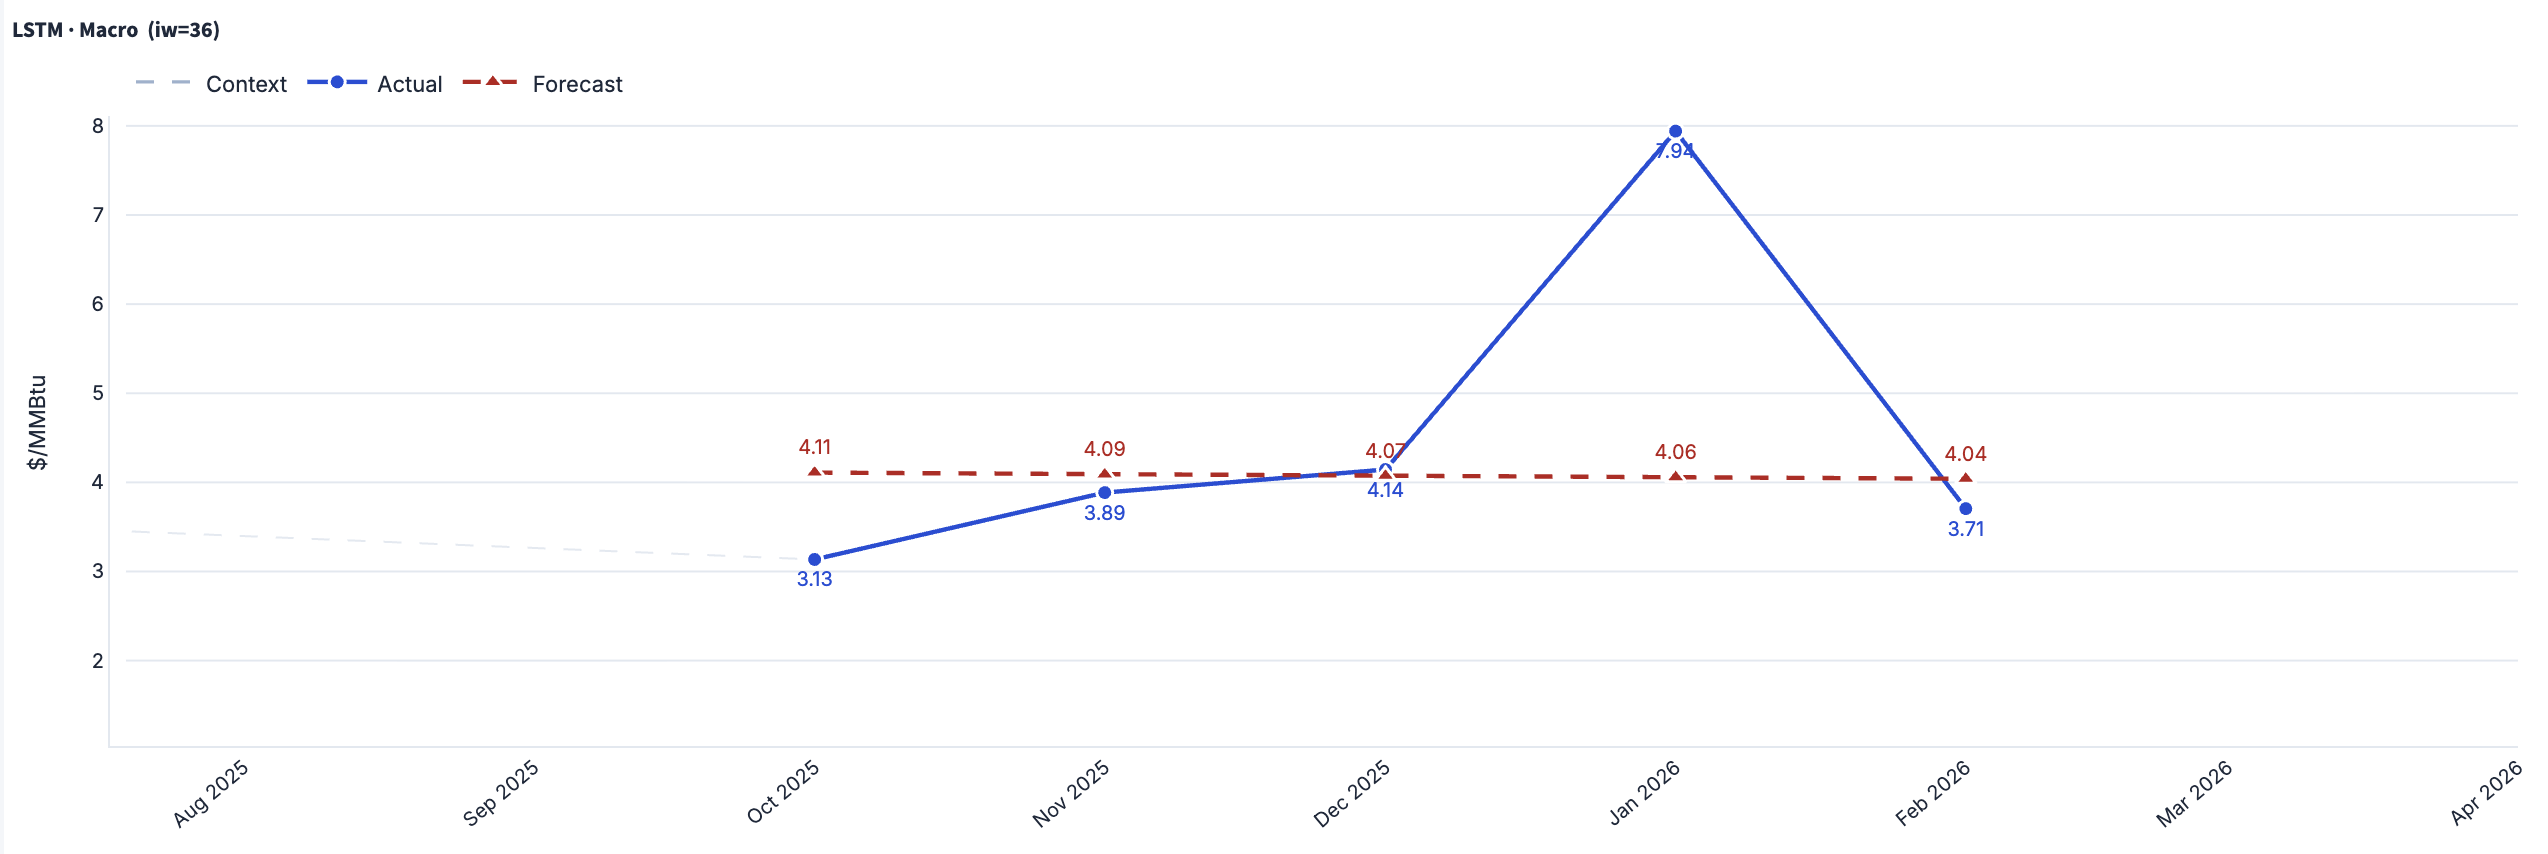
\includegraphics[width=\textwidth]{figures/multivariate_macro_cng_lstm.png}
\small (b) LSTM forecast for natural gas
\end{minipage}

\vspace{0.5em}

\begin{minipage}[t]{0.48\textwidth}
\centering
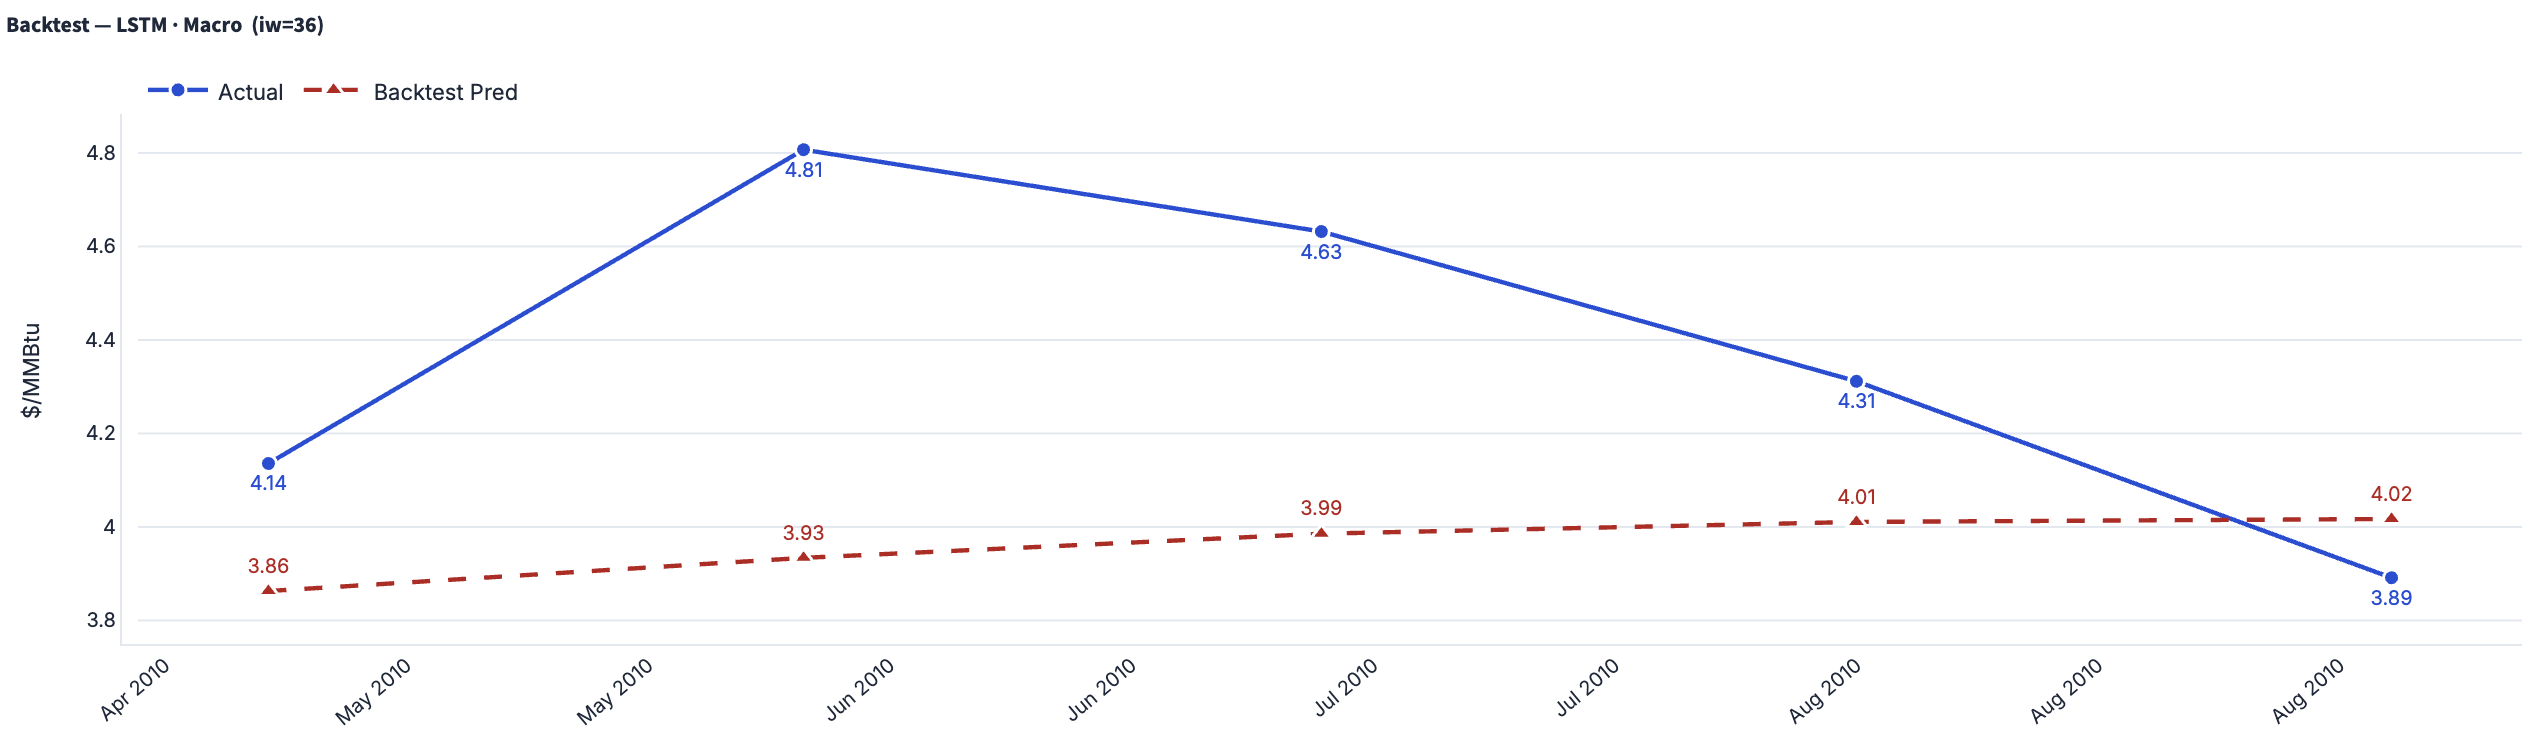
\includegraphics[width=\textwidth]{figures/multivariate_macro_cng_lstm_backtest.png}
\small (c) LSTM backtest for natural gas
\end{minipage}\hfill
\begin{minipage}[t]{0.48\textwidth}
\centering
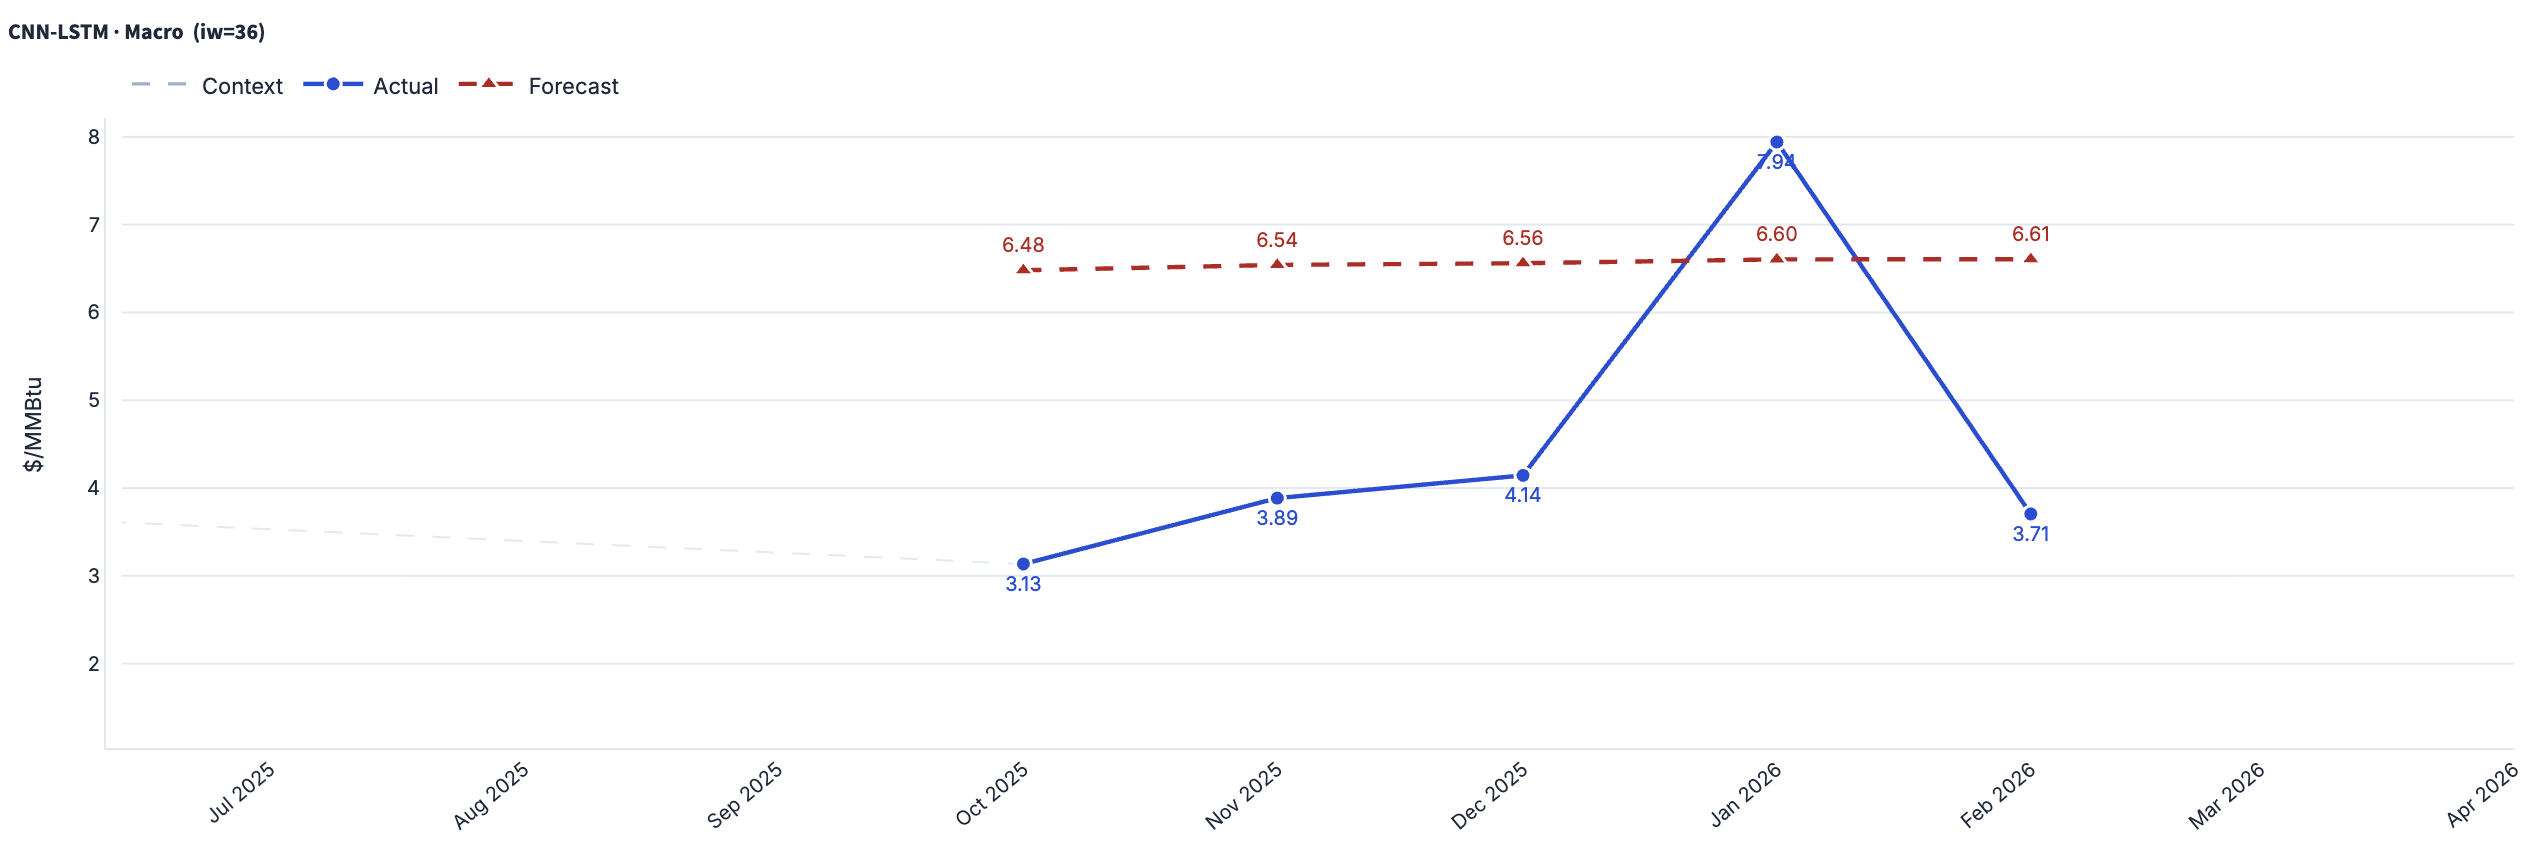
\includegraphics[width=\textwidth]{figures/multivariate_macro_cng_cnnlstm.png}
\small (d) CNN--LSTM forecast for natural gas
\end{minipage}

\vspace{0.5em}

\begin{minipage}[t]{0.48\textwidth}
\centering
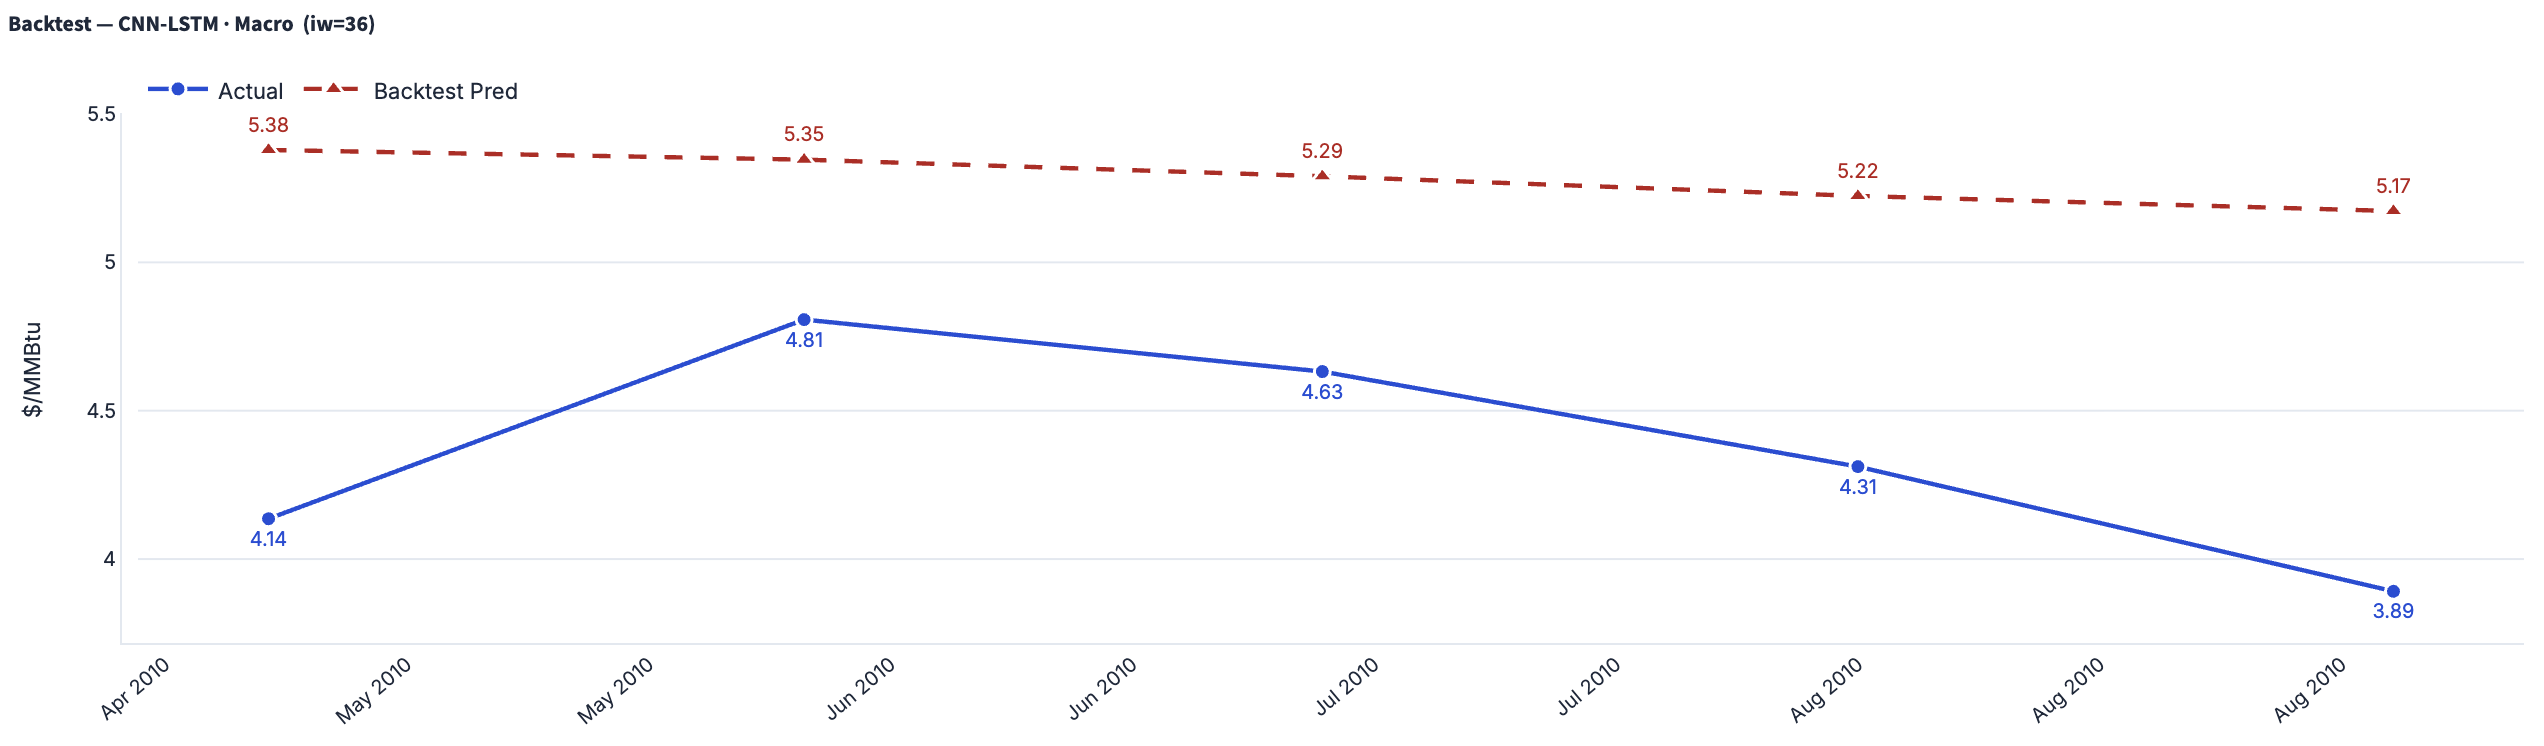
\includegraphics[width=\textwidth]{figures/multivariate_macro_cng_cnnlstm_backtest.png}
\small (e) CNN--LSTM backtest for natural gas
\end{minipage}
\caption{Actual versus predicted Henry Hub natural gas prices (USD/MMBtu) using macroeconomic variables only: (a) SARIMAX forecast with exogenous FRED indicators, (b) LSTM direct forecast, (c) LSTM walk-forward backtest, (d) CNN--LSTM direct forecast, and (e) CNN--LSTM walk-forward backtest. This figure summarizes the macro-only multivariate setting.}
\label{fig:macro_only_cng_plots}
\end{figure}

\begin{table}[h]
\centering
\caption{Macro-only multivariate model performance for natural gas}
\label{tab:macro_only_cng}
\begin{tabular}{@{}lcccc@{}}
\toprule
Model & RMSE (USD/MMBtu) & MAE (USD/MMBtu) & MAPE (\%) & DA \\
\midrule
SARIMAX & 1.532 & 1.158 & 42.20 & 0.20 \\
LSTM Forecast & 1.800 & 1.093 & 19.19 & 0.40 \\
LSTM Backtest & 0.522 & 0.444 & 9.79 & 0.25 \\
CNN--LSTM Forecast & 2.619 & 2.532 & 65.72 & 0.60 \\
CNN--LSTM Backtest & 0.974 & 0.927 & 21.91 & 0.00 \\
\botrule
\end{tabular}
\end{table}

As shown in Figure~\ref{fig:macro_only_cng_plots}, macroeconomic variables alone provide limited predictive capability for natural gas prices. SARIMAX again records relatively high error, indicating that a linear multivariate specification is not sufficient to explain the observed movement in the series. The LSTM model delivers more moderate forecasting performance and comparatively stable backtesting results, suggesting that it models part of the temporal structure, although not strongly enough to track the series consistently.

The CNN--LSTM model performs poorly in direct forecasting despite achieving the highest DA in this setting (0.60), which points to inconsistency in what the model learns across evaluation settings. The LSTM backtest lowers RMSE to 0.522, but its DA remains only 0.25, while the CNN--LSTM backtest drops to 0.00. More broadly, the figure shows that none of the macro-only models are able to follow actual natural gas price movements in a consistently reliable way. Across both crude oil and natural gas, these findings suggest that macroeconomic variables used in isolation are not sufficiently predictive of short-term energy price dynamics. While the neural architectures show some ability to reproduce local patterns, their performance remains unstable across forecasting and backtesting, reinforcing the need to incorporate additional information sources, particularly news-based signals, in the subsequent multivariate settings.

For natural gas, however, the DM evidence is weaker. None of the macro-only pairwise comparisons reaches conventional significance levels: SARIMAX versus LSTM yields $p=0.160$, SARIMAX versus CNN--LSTM yields $p=0.080$, and LSTM versus CNN--LSTM yields $p=0.270$. This suggests that although some models appear numerically better in RMSE or DA terms, the macro-only CNG differences are not statistically robust enough to establish a clear winner.

\subsubsection*{5.2.2 News Only}

We designed this setting to evaluate the standalone contribution of news-derived signals. We conducted the experiments using only features extracted from the GDELT dataset, including aggregated event counts, average tone, and the Goldstein scale, which together reflect event-driven and sentiment-based information.

Given the highly dynamic and unstructured nature of news data, we selected the CNN--LSTM architecture for this setting. The convolutional component models local temporal patterns across event features, while the LSTM layer models sequential dependencies over time. For crude oil, the model was trained using an input window of 24 time steps and a multi-step output of 5 steps in a one-shot forecasting setting. For natural gas, an input window of 36 time steps with a single-step output was used.

\subsubsection*{5.2.2.1 Crude Oil}
For crude oil, Table~\ref{tab:news_only_oil} summarizes the performance of the news-only CNN--LSTM model, and Figure~\ref{fig:news_only_oil_plots} shows the corresponding forecast and backtest plots.

\begin{figure}[h]
\centering
\begin{minipage}[t]{0.48\textwidth}
\centering
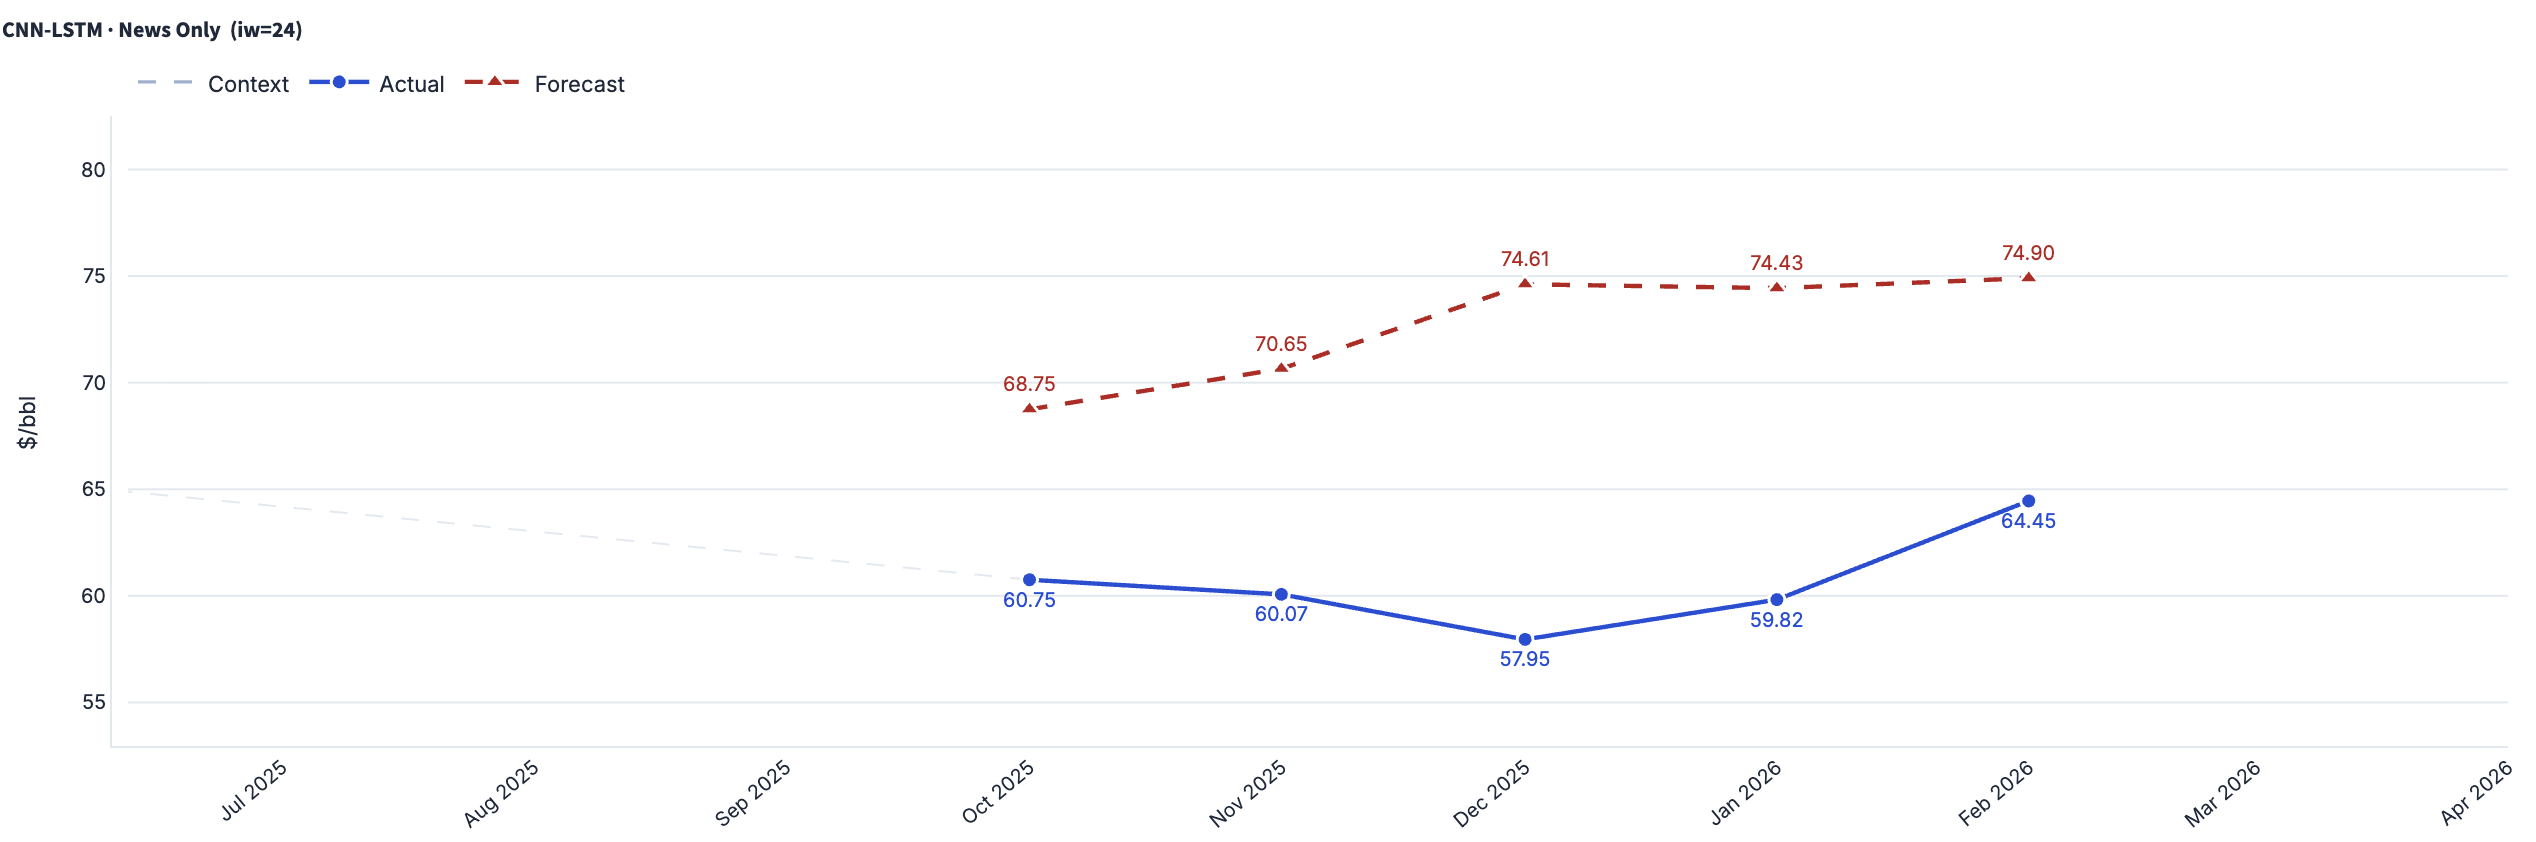
\includegraphics[width=\textwidth]{figures/multivariate_oil_news_cnn_lstm.png}
\small (a) CNN--LSTM forecast for crude oil using news features
\end{minipage}\hfill
\begin{minipage}[t]{0.48\textwidth}
\centering
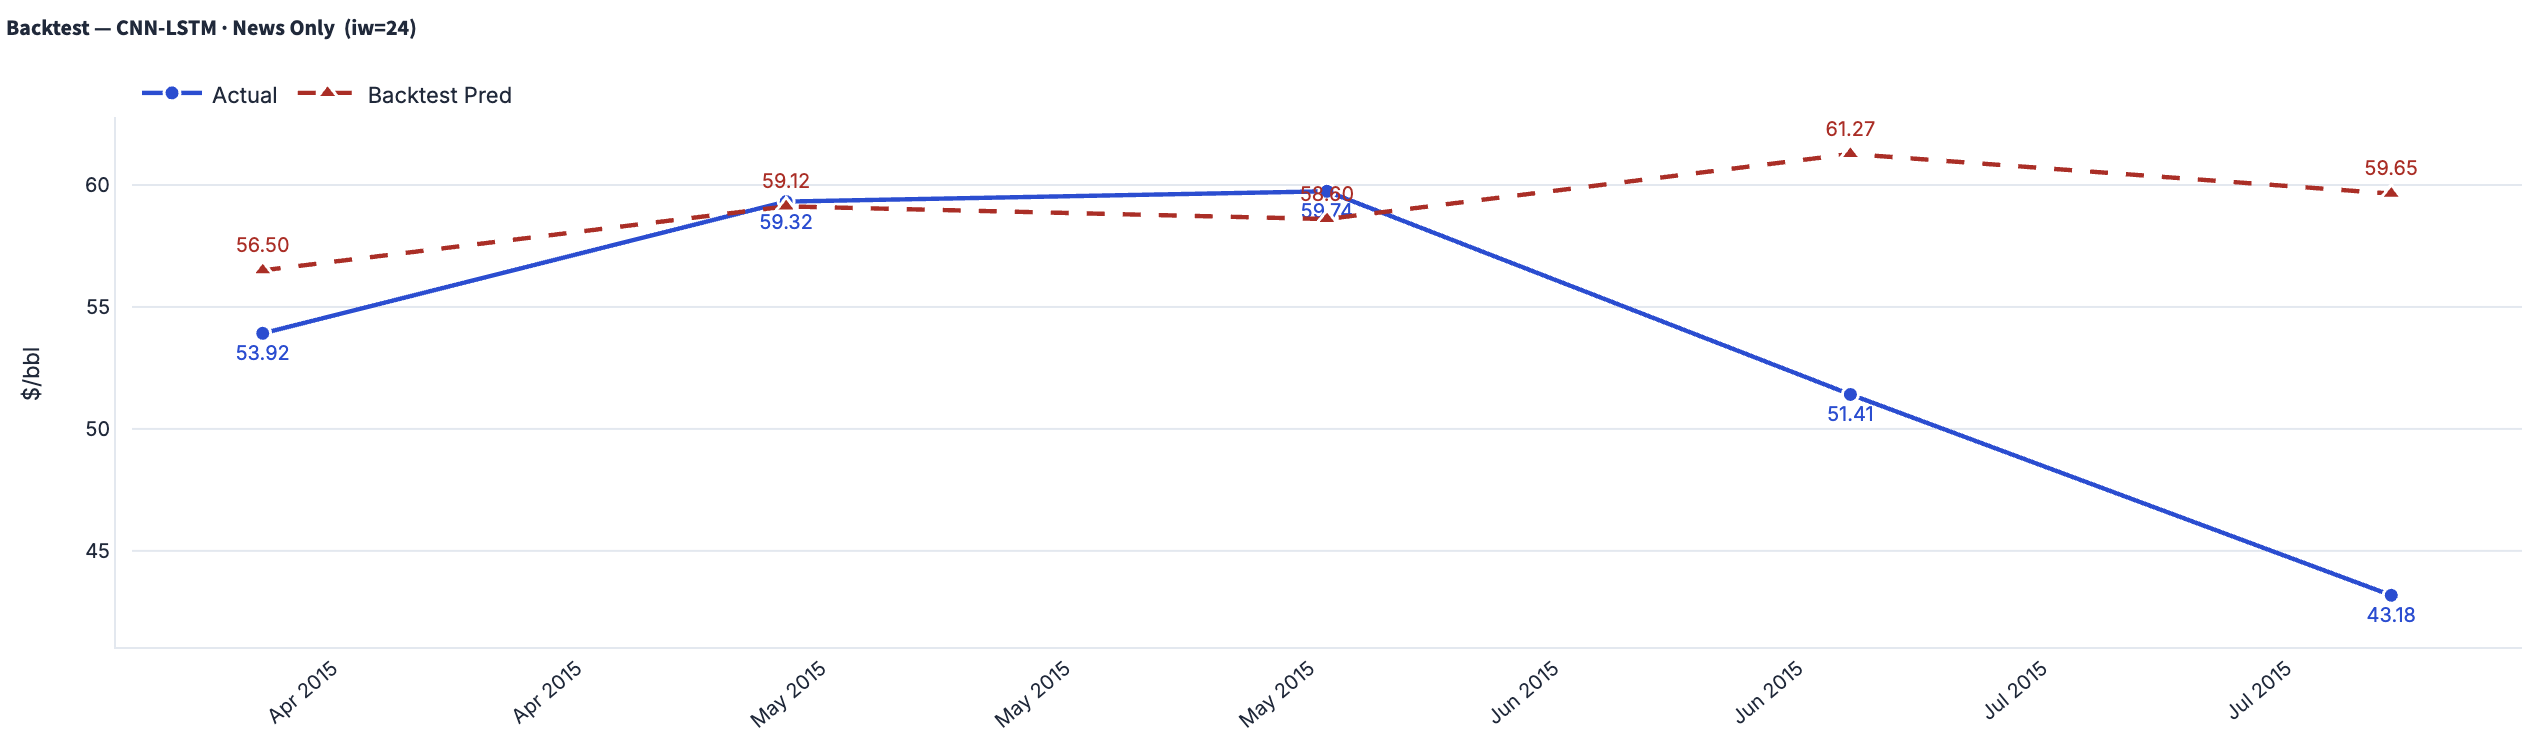
\includegraphics[width=\textwidth]{figures/multivariate_oil_news_cnn_lstm_backtest.png}
\small (b) CNN--LSTM backtest for crude oil using news features
\end{minipage}
\caption{Actual versus predicted WTI crude oil prices (USD/barrel) using only GDELT-derived news features in the CNN--LSTM setting: (a) direct forecast and (b) walk-forward backtest. The panels summarize the standalone contribution of event-count, tone, and Goldstein-scale signals without macroeconomic inputs.}
\label{fig:news_only_oil_plots}
\end{figure}

\begin{table}[h]
\centering
\caption{News-only model performance for crude oil}
\label{tab:news_only_oil}
\begin{tabular}{@{}lcccc@{}}
\toprule
Model & RMSE (USD/barrel) & MAE (USD/barrel) & MAPE (\%) & DA \\
\midrule
CNN--LSTM Forecast & 12.459 & 12.060 & 20.03 & 0.60 \\
CNN--LSTM Backtest & 8.676 & 6.049 & 12.87 & 0.40 \\
\botrule
\end{tabular}
\end{table}

Figure~\ref{fig:news_only_oil_plots} indicates that the news-only CNN--LSTM model is able to track some variation in crude oil prices, suggesting that event-driven signals do contain useful information. However, the forecasting errors remain relatively high, and the model does not align consistently with the observed price path. The forecast tracks the broad direction of movement in some periods, but it struggles to match sharp fluctuations and exact price levels.

The backtesting results show moderate improvement relative to the direct forecast, but the error remains large enough to suggest that the model is not sufficiently reliable on its own. In directional terms, the forecast DA of 0.60 is stronger than the backtest DA of 0.40, indicating that the news-only model reflects some broad sign changes for crude oil but cannot do so consistently across rolling windows. In substantive terms, the figure shows a model that can reflect general market shifts associated with news flow, yet lacks the precision needed for dependable short-term forecasting. Economically, this is plausible because oil prices respond not only to headlines but also to inventories, production quotas, and transport constraints that aggregated news features do not fully represent. This suggests that while news-derived signals carry relevant information for crude oil, they are not strong enough in isolation to fully explain the dynamics of the series.

The DM results are consistent with that reading. None of the news-only crude-oil pairwise comparisons is statistically significant, with $p=0.230$ for SARIMAX versus LSTM, $p=0.200$ for SARIMAX versus CNN--LSTM, and $p=0.510$ for LSTM versus CNN--LSTM. Accordingly, the news-only setting does not provide statistically reliable evidence that one model dominates the others for crude oil.

\subsubsection*{5.2.2.2 Natural Gas (CNG)}
For natural gas, Table~\ref{tab:news_only_cng} reports the news-only CNN--LSTM results, and Figure~\ref{fig:news_only_cng_plots} illustrates them.

\begin{figure}[h]
\centering
\begin{minipage}[t]{0.48\textwidth}
\centering
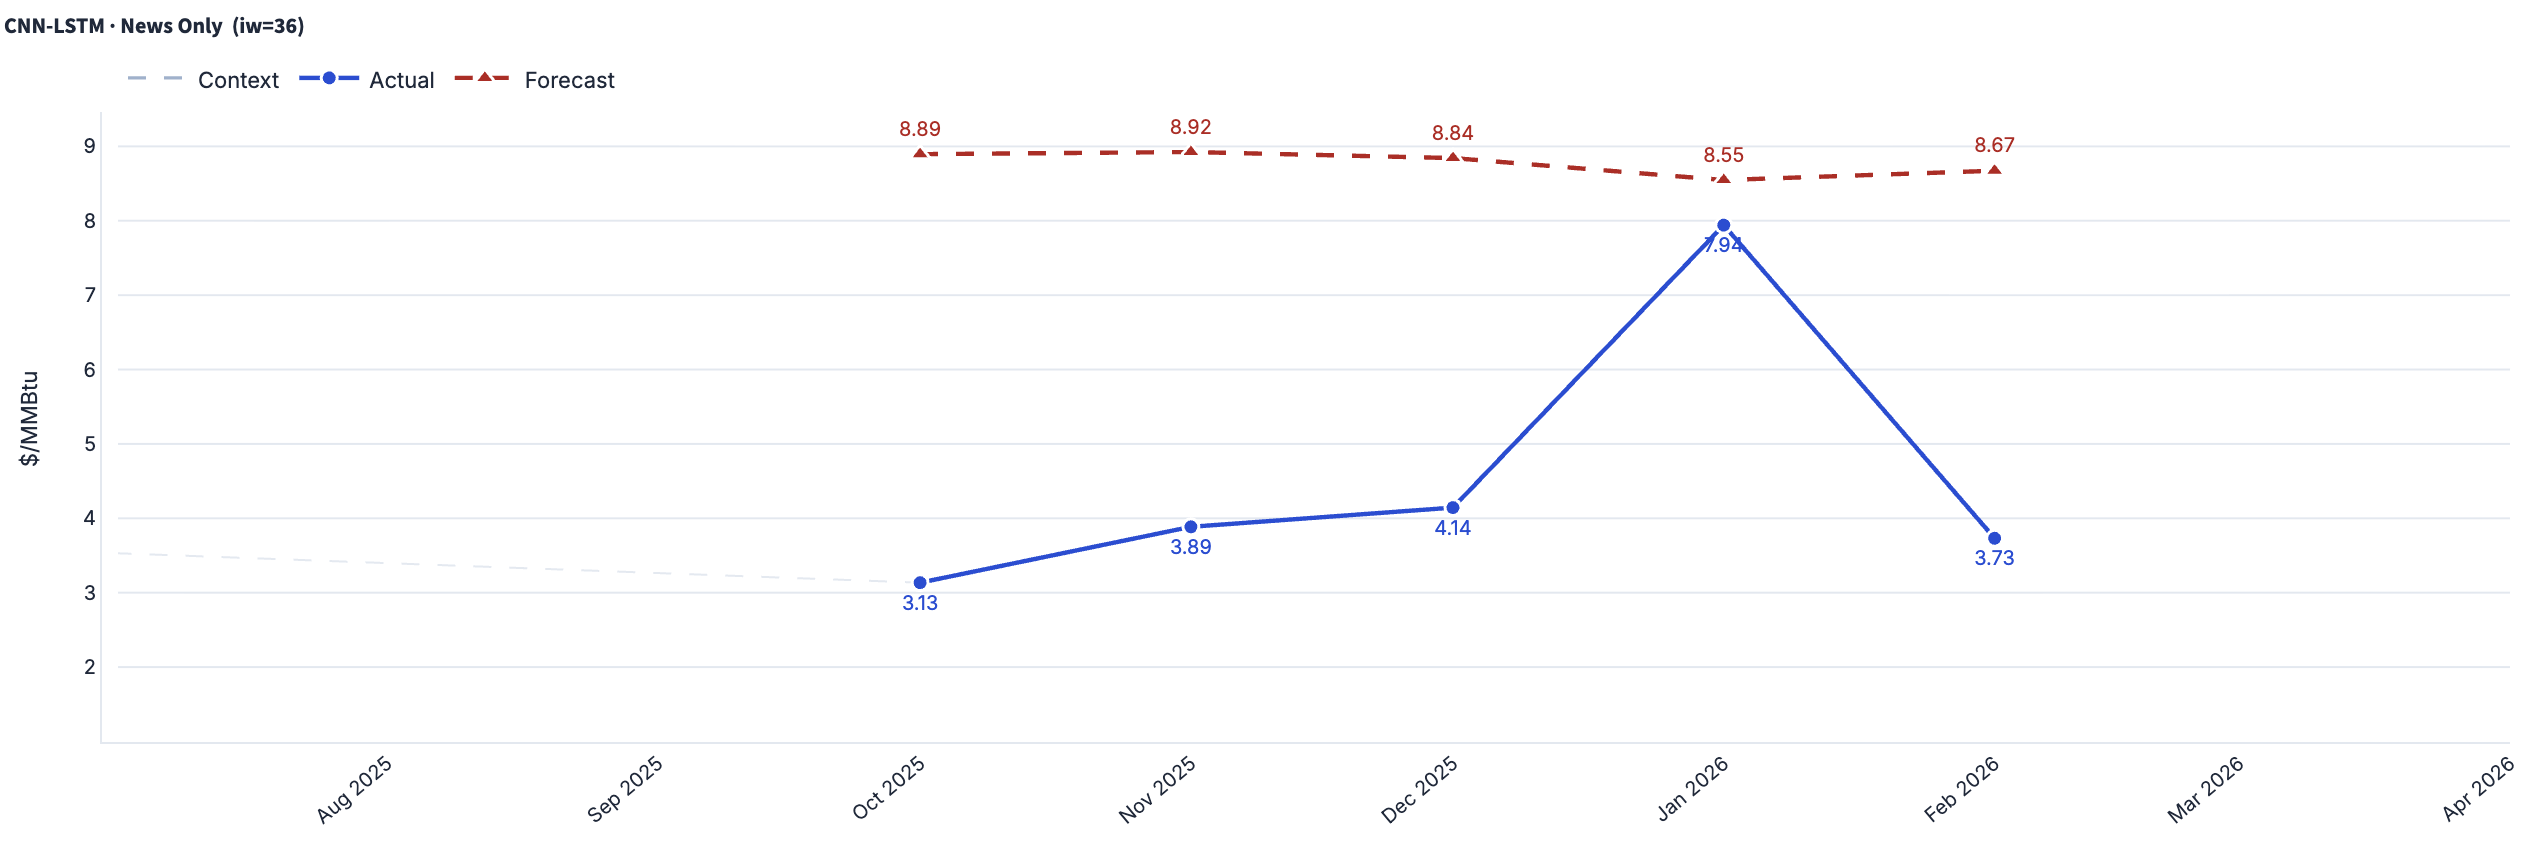
\includegraphics[width=\textwidth]{figures/multivariate_cng_news_cnn_lstm.png}
\small (a) CNN--LSTM forecast for natural gas using news features
\end{minipage}\hfill
\begin{minipage}[t]{0.48\textwidth}
\centering
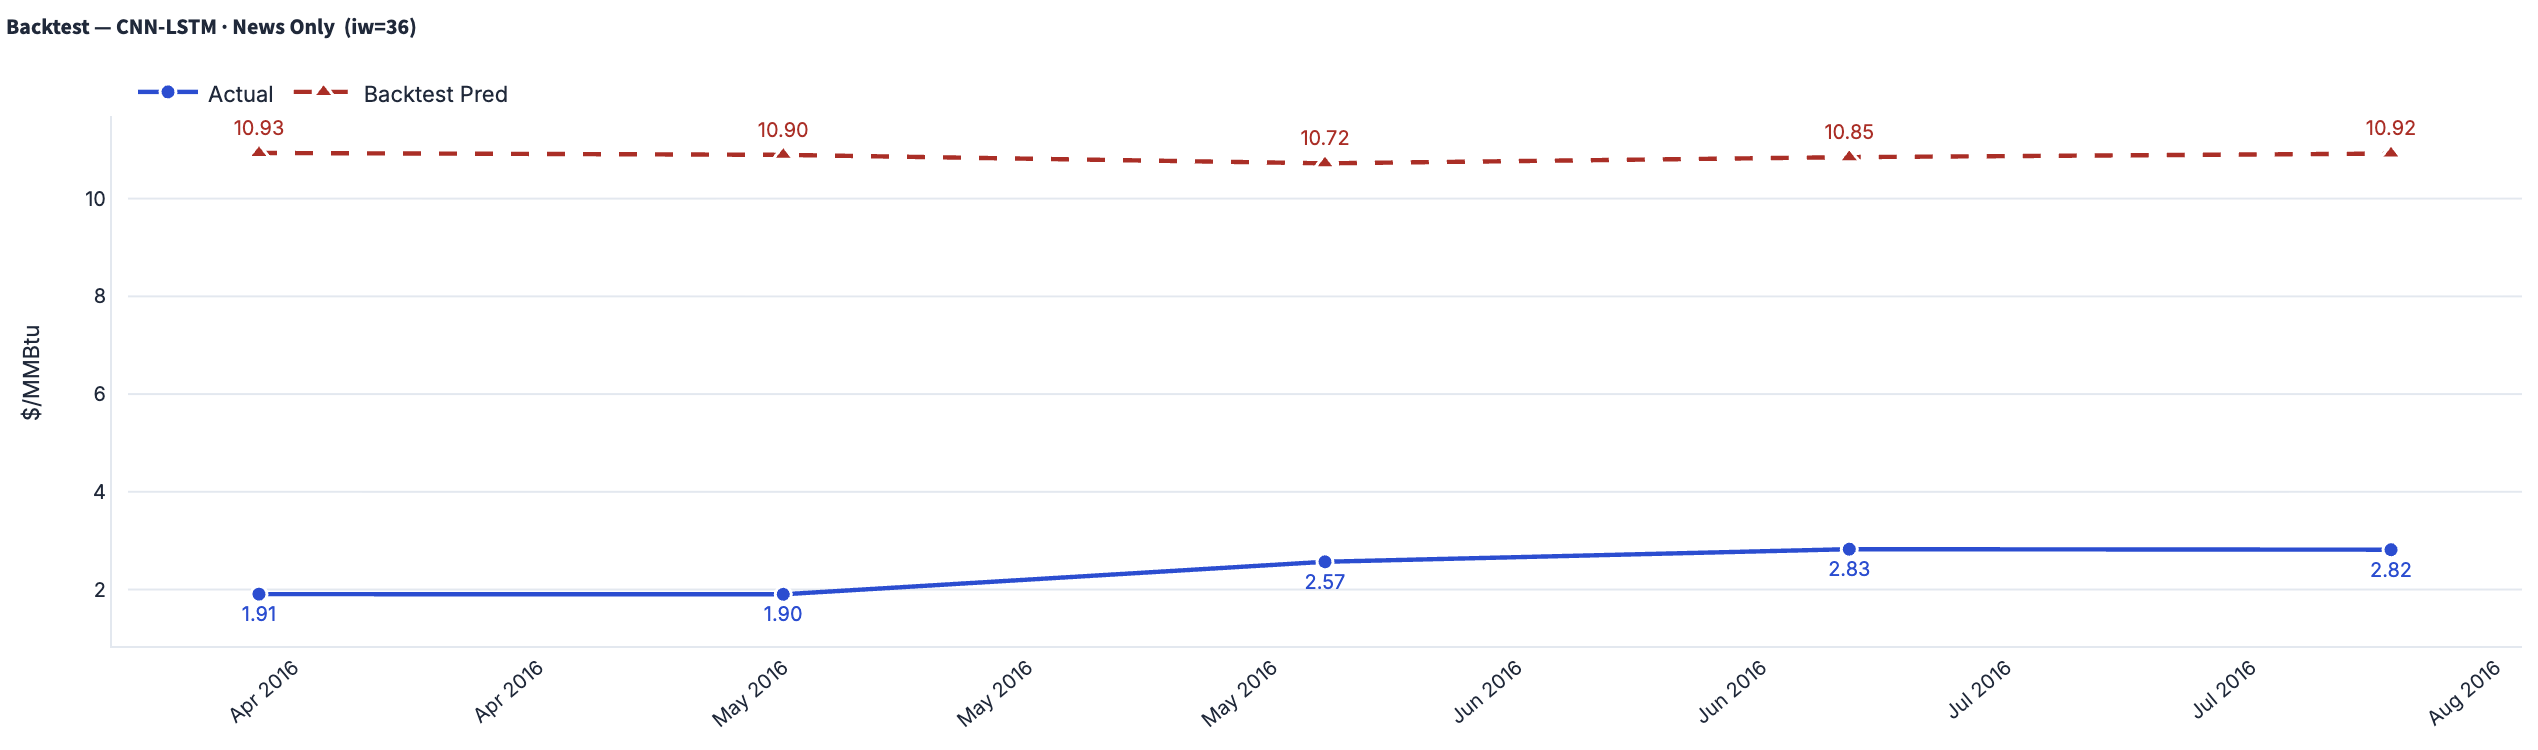
\includegraphics[width=\textwidth]{figures/multivariate_cng_news_cnn_lstm_backtest.png}
\small (b) CNN--LSTM backtest for natural gas using news features
\end{minipage}
\caption{Actual versus predicted Henry Hub natural gas prices (USD/MMBtu) using only GDELT-derived news features in the CNN--LSTM setting: (a) direct forecast and (b) walk-forward backtest. The panels summarize the standalone contribution of event-count, tone, and Goldstein-scale signals without macroeconomic inputs.}
\label{fig:news_only_cng_plots}
\end{figure}

\begin{table}[h]
\centering
\caption{News-only model performance for natural gas}
\label{tab:news_only_cng}
\begin{tabular}{@{}lcccc@{}}
\toprule
Model & RMSE (USD/MMBtu) & MAE (USD/MMBtu) & MAPE (\%) & DA \\
\midrule
CNN--LSTM Forecast & 4.592 & 4.209 & 113.37 & 0.40 \\
CNN--LSTM Backtest & 8.473 & 8.461 & 367.16 & 0.00 \\
\botrule
\end{tabular}
\end{table}

As shown in Figure~\ref{fig:news_only_cng_plots}, the performance of the news-only model for natural gas is substantially weaker than for crude oil. Both forecasting and backtesting errors are high, indicating that news-derived features alone are insufficient to explain natural gas price movements in a stable or accurate way. The predictions deviate markedly from the observed series and fail to reproduce both the direction and magnitude of many changes. The DA results confirm this weakness, dropping from 0.40 in the direct forecast to 0.00 in backtesting.

This pattern suggests that, for natural gas, the information contained in aggregated news signals is too indirect or too noisy to support reliable standalone forecasting. Compared with crude oil, where news appears to offer at least some useful directional information, the CNG results point to a much weaker connection between the extracted GDELT features and short-term price behavior.

The DM test reinforces this conclusion for natural gas. All three news-only pairwise comparisons are clearly non-significant, with p-values of 0.360, 0.290, and 0.610, respectively. Thus, in addition to having large forecast errors, the news-only CNG models do not exhibit statistically distinguishable predictive accuracy in this subsection.

Taken together, the news-only results show that event-driven signals are informative but not sufficient on their own for robust energy price forecasting. For crude oil, the CNN--LSTM model tracks broad movements but lacks precision. For natural gas, performance is considerably weaker, indicating that news signals alone do not adequately represent the underlying price dynamics. These findings suggest that news-based features are more useful as complementary inputs than as standalone predictors, and they motivate the combined macro-plus-news setting examined next.

\subsubsection*{5.2.3 Macro + News Combined Model}

To address the limitations observed in the macro-only and news-only settings, both feature groups were combined in a unified multivariate framework. Macroeconomic variables provide structured long-term trends, while news-derived features introduce event-driven and sentiment-based dynamics. By integrating these two sources, we intend the combined setup to reflect complementary information that neither group can provide on its own.

We evaluated this framework using SARIMAX, LSTM, and CNN--LSTM models. For the neural architectures, the sequence configurations were defined as follows: for crude oil, LSTM used a 24-step input and 5-step output, while CNN--LSTM used a 36-step input and 5-step output; for natural gas, both LSTM and CNN--LSTM used a 36-step input and 5-step output. SARIMAX was implemented with monthly modeling for crude oil and daily modeling for natural gas.

\subsubsection*{5.2.3.1 Crude Oil}
Table~\ref{tab:combined_oil} summarizes the performance of the combined-feature models for crude oil, and Figure~\ref{fig:combined_oil_plots} presents the corresponding prediction plots.

\begin{figure}[h]
\centering
\begin{minipage}[t]{0.48\textwidth}
\centering
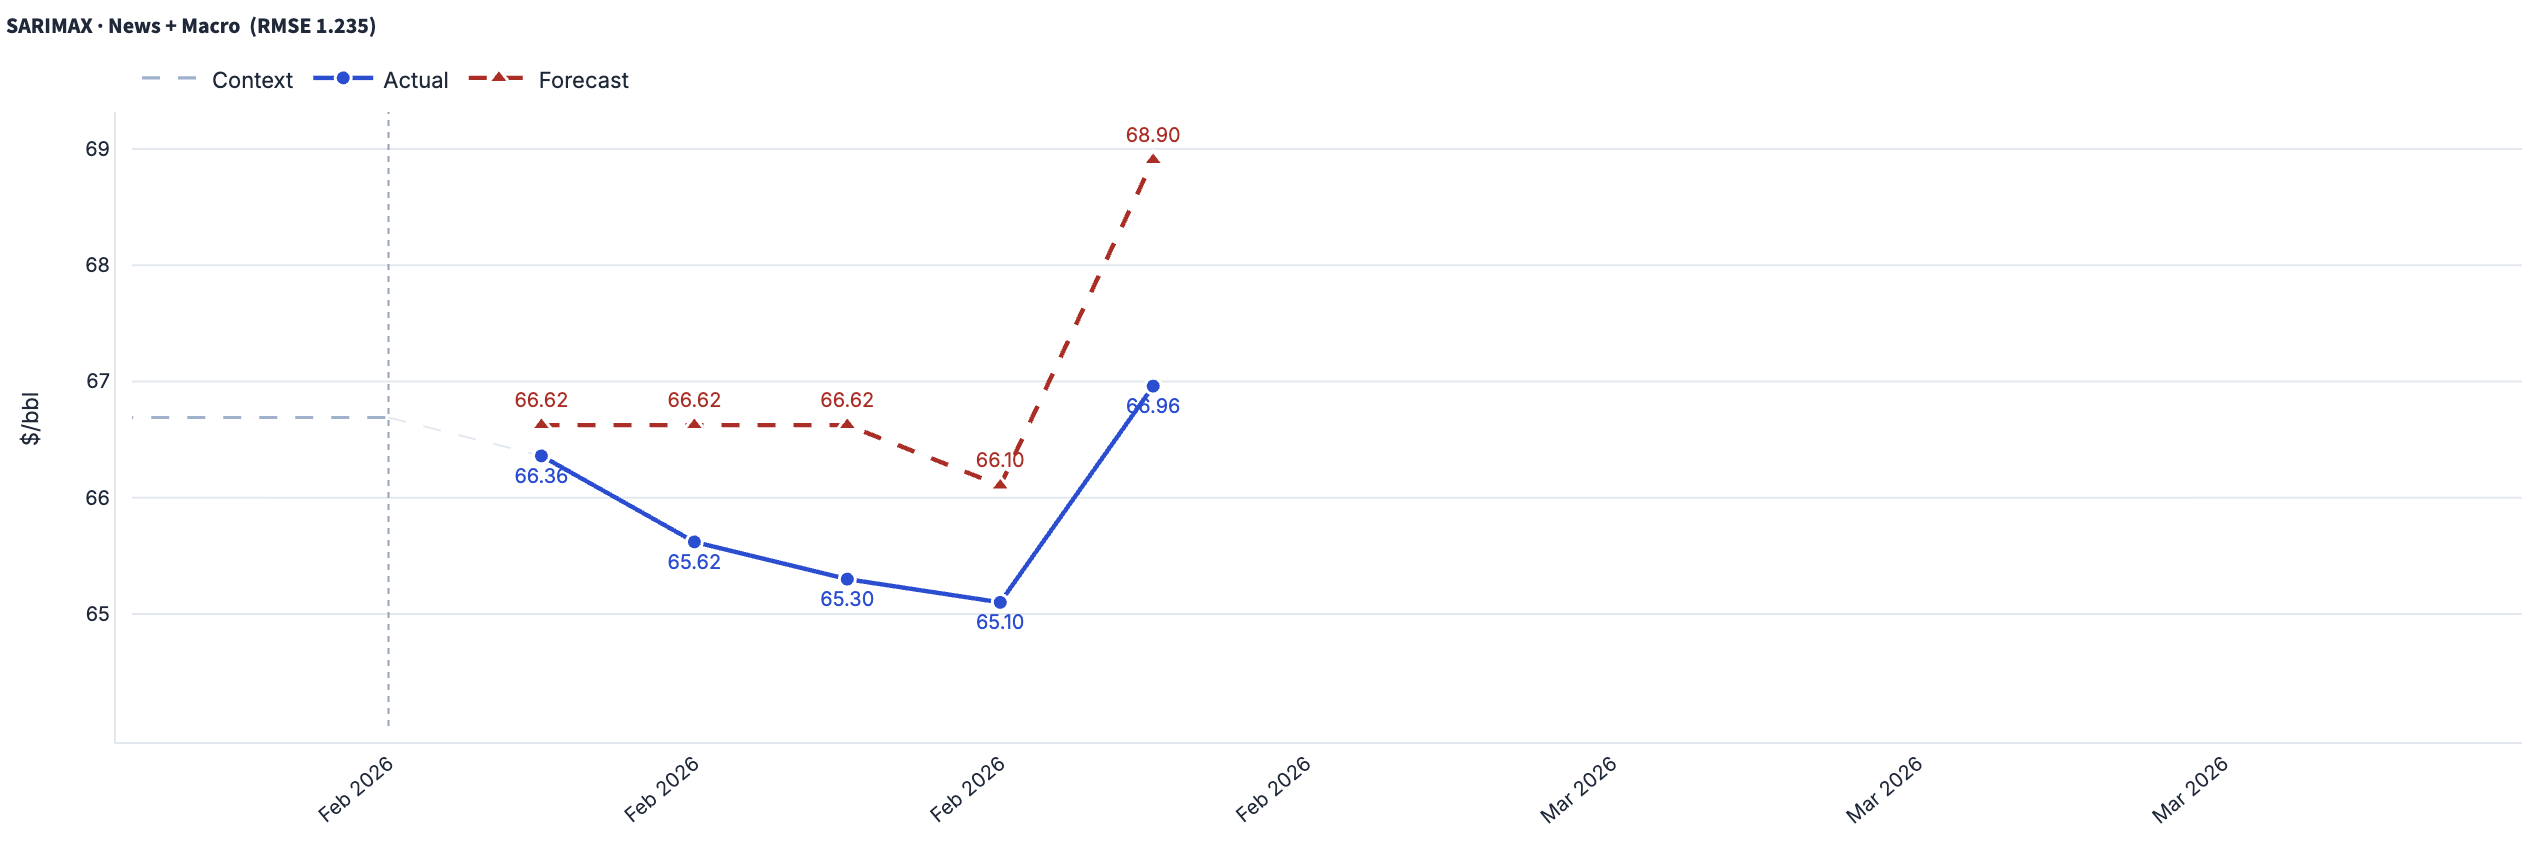
\includegraphics[width=\textwidth]{figures/multivariate_news_macro_oil_sarimax.png}
\small (a) SARIMAX forecast for crude oil
\end{minipage}\hfill
\begin{minipage}[t]{0.48\textwidth}
\centering
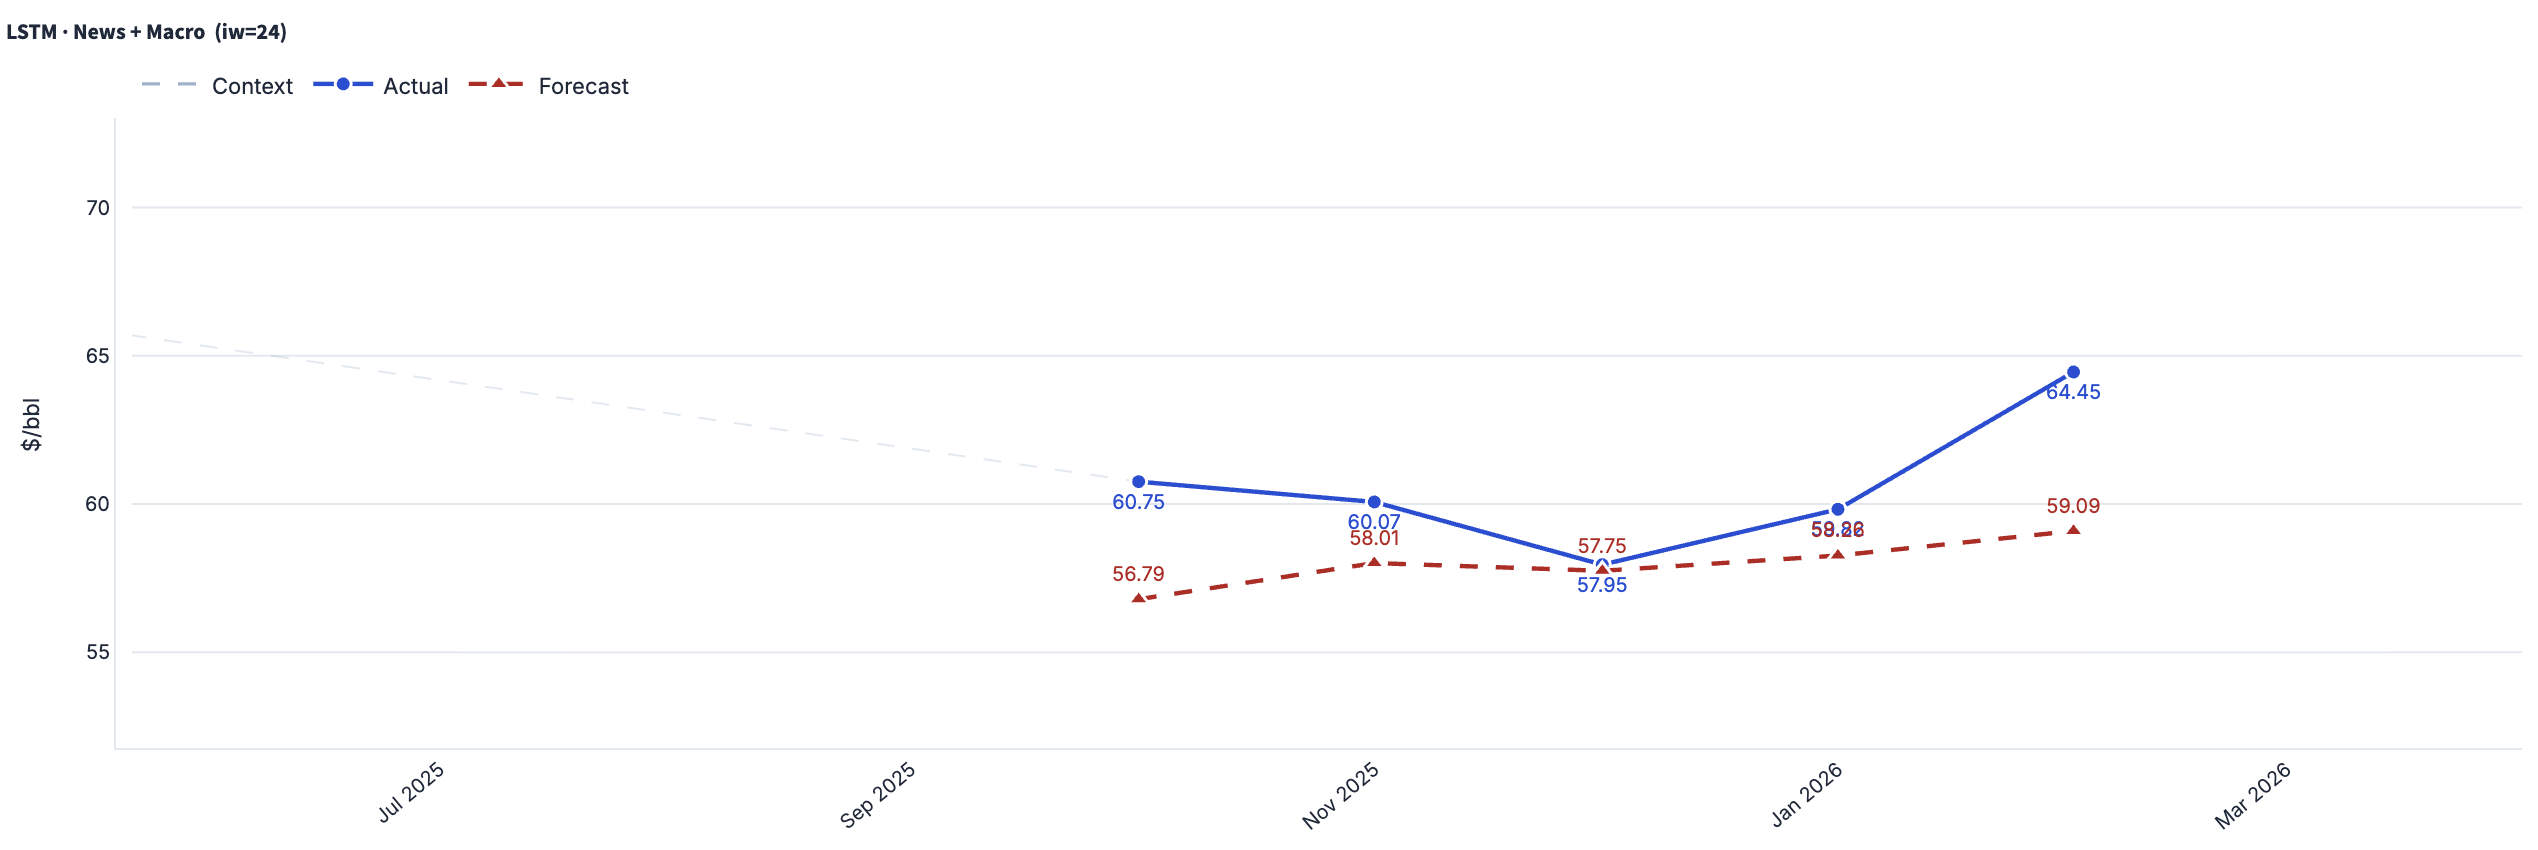
\includegraphics[width=\textwidth]{figures/multivariate_news_macro_oil_lstm.png}
\small (b) LSTM forecast for crude oil
\end{minipage}

\vspace{0.5em}

\begin{minipage}[t]{0.48\textwidth}
\centering
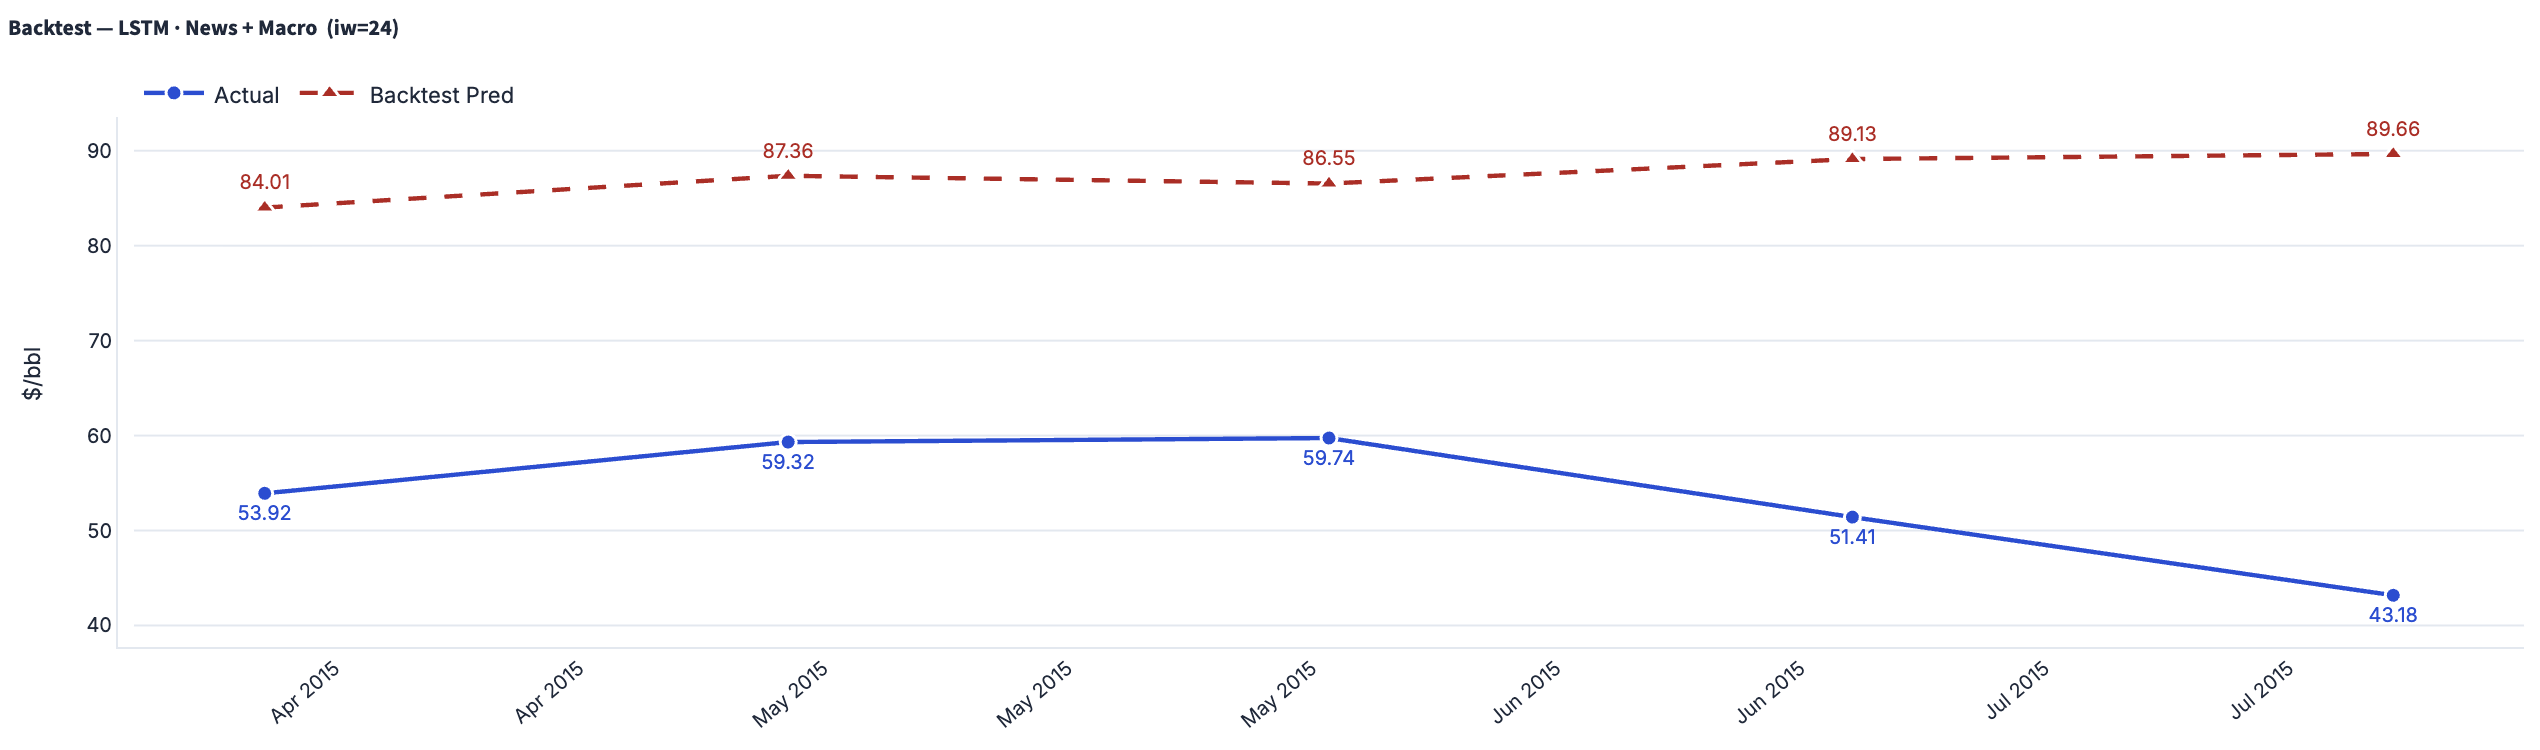
\includegraphics[width=\textwidth]{figures/multivariate_news_macro_oil_lstm_backtest.png}
\small (c) LSTM backtest for crude oil
\end{minipage}\hfill
\begin{minipage}[t]{0.48\textwidth}
\centering
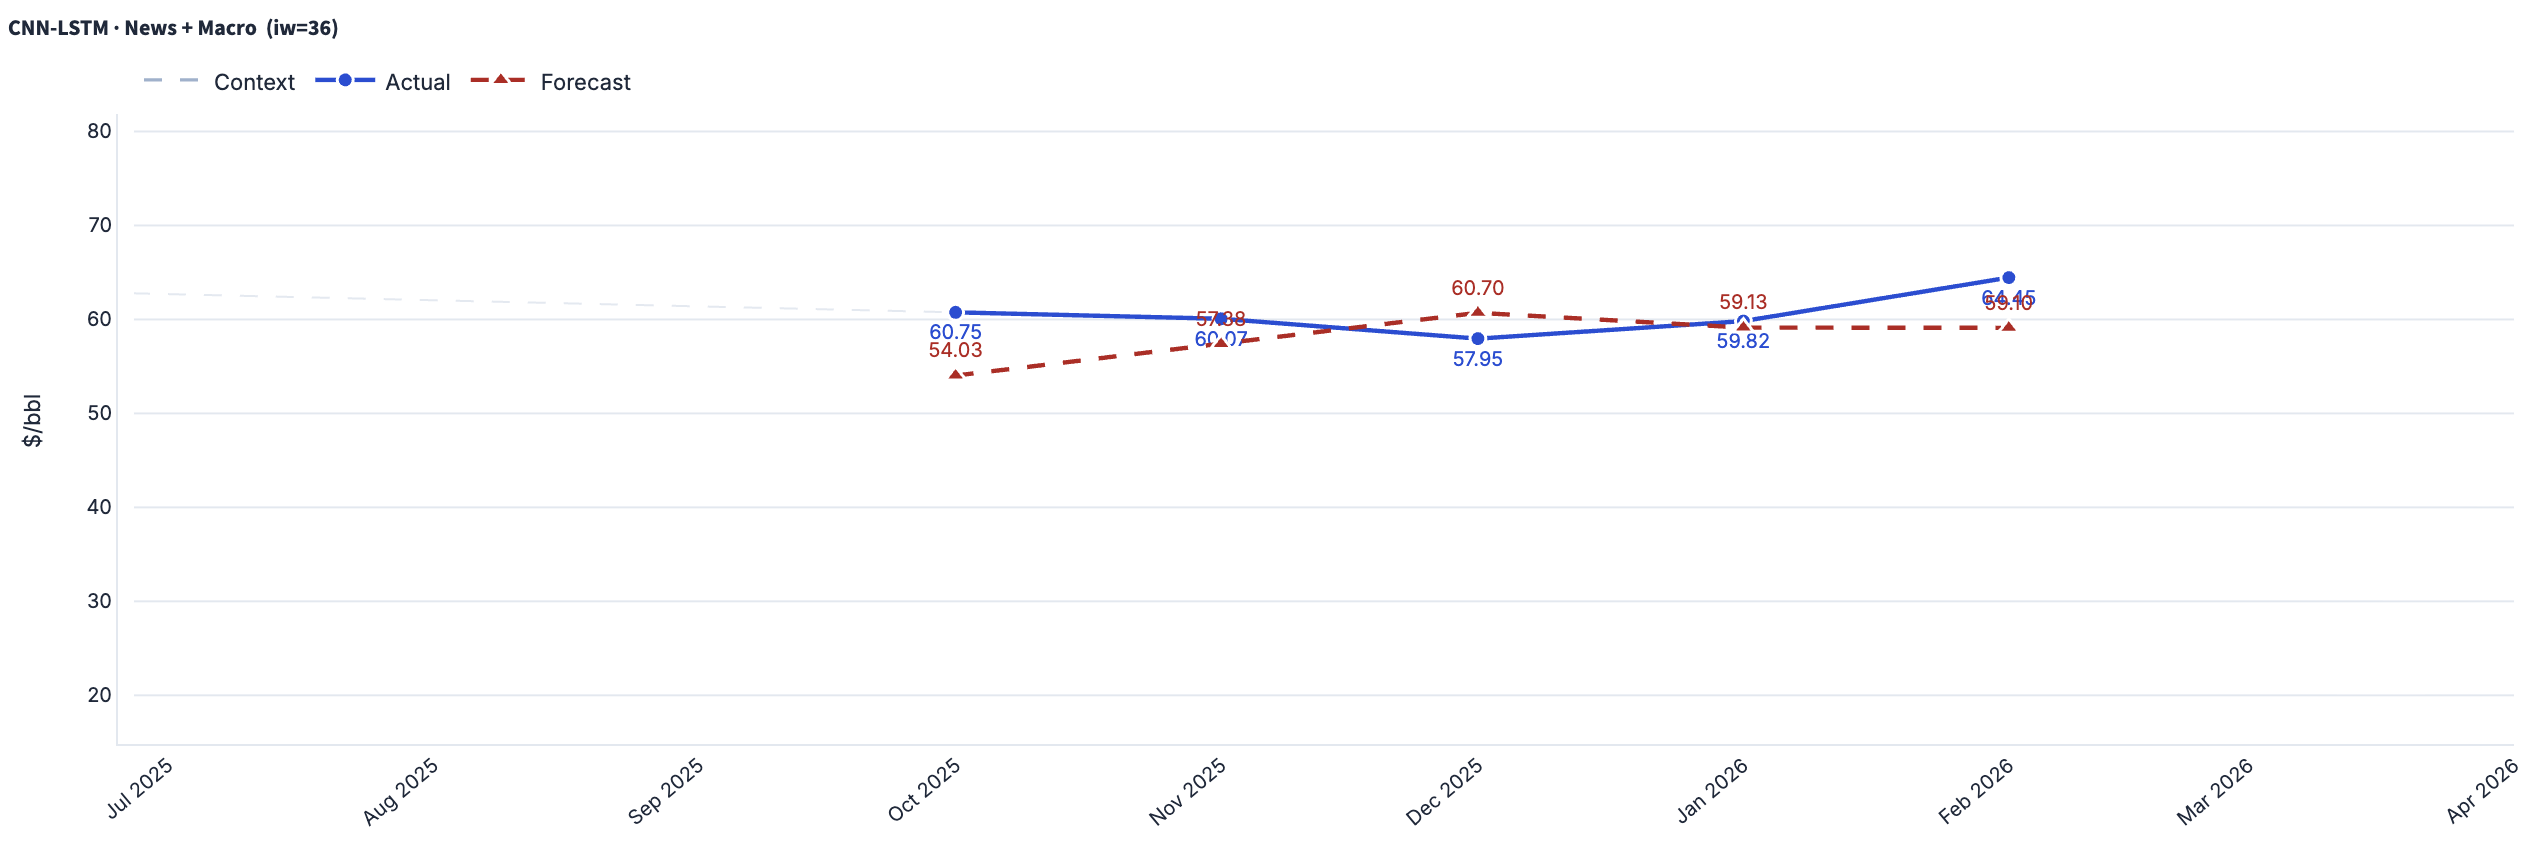
\includegraphics[width=\textwidth]{figures/multivariate_news_macro_oil_cnnlstm.png}
\small (d) CNN--LSTM forecast for crude oil
\end{minipage}

\vspace{0.5em}

\begin{minipage}[t]{0.48\textwidth}
\centering
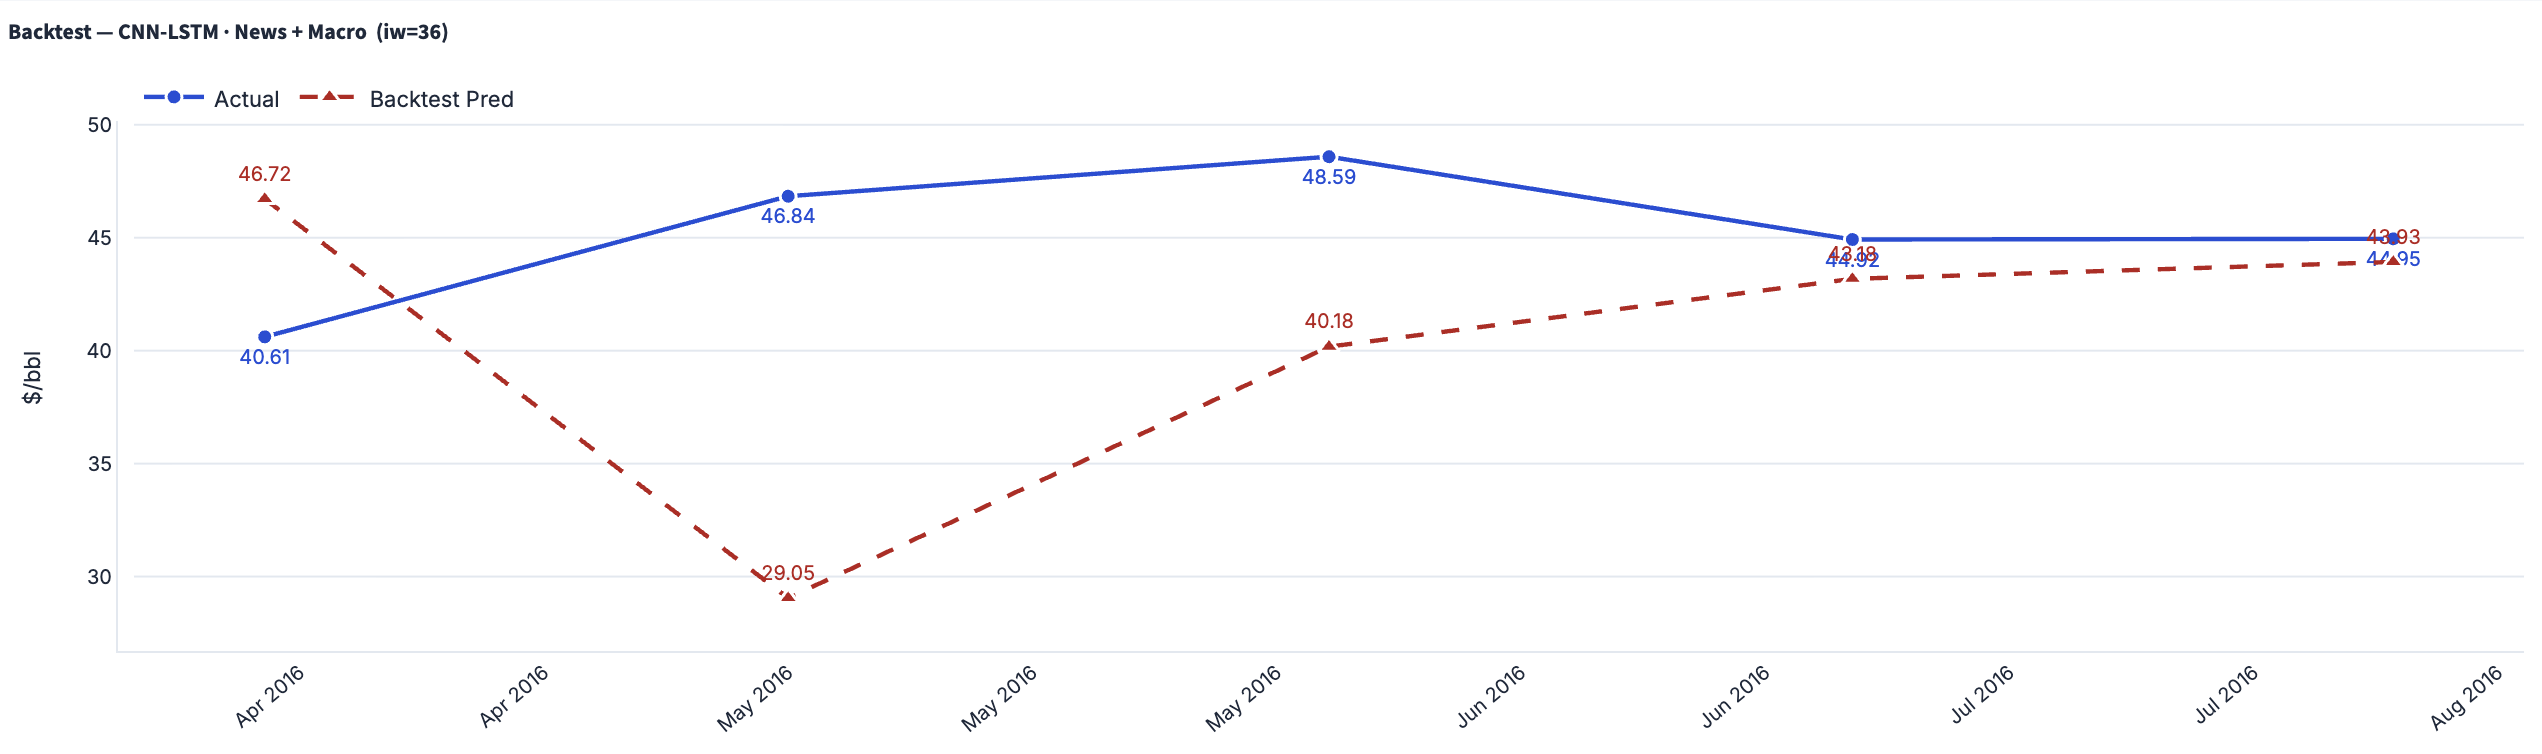
\includegraphics[width=\textwidth]{figures/multivariate_news_macro_oil_cnnlstm_backtest.png}
\small (e) CNN--LSTM backtest for crude oil
\end{minipage}
\caption{Actual versus predicted WTI crude oil prices (USD/barrel) using the combined macroeconomic and GDELT-derived news feature set: (a) SARIMAX forecast, (b) LSTM direct forecast, (c) LSTM walk-forward backtest, (d) CNN--LSTM direct forecast, and (e) CNN--LSTM walk-forward backtest. This figure summarizes the joint-feature multivariate setting.}
\label{fig:combined_oil_plots}
\end{figure}

\begin{table}[h]
\centering
\caption{Combined macro-plus-news model performance for crude oil}
\label{tab:combined_oil}
\begin{tabular}{@{}lcccc@{}}
\toprule
Model & RMSE (USD/barrel) & MAE (USD/barrel) & MAPE (\%) & DA \\
\midrule
SARIMAX & 1.235 & 1.109 & 1.68 & 0.60 \\
LSTM Forecast & 3.200 & 2.631 & 4.25 & 0.40 \\
LSTM Backtest & 34.622 & 33.828 & 65.79 & 0.00 \\
CNN--LSTM Forecast & 4.223 & 3.641 & 5.95 & 0.80 \\
CNN--LSTM Backtest & 9.257 & 7.014 & 15.30 & 0.60 \\
\botrule
\end{tabular}
\end{table}

The combined feature setting leads to a substantial improvement for crude oil, particularly for SARIMAX, which achieves very low error values relative to the previous settings. This suggests that once macroeconomic trends and news signals are used together, the linear model is able to identify substantive relationships that are not visible when either feature group is used in isolation. Figure~\ref{fig:combined_oil_plots} supports this interpretation, as the SARIMAX predictions follow the observed series closely and track the major movements with comparatively little deviation. Directionally, however, the CNN--LSTM forecast attains the highest DA at 0.80, while SARIMAX still remains strong at 0.60.

The LSTM model shows reasonable forecasting performance, but its backtesting error increases sharply, indicating instability across different temporal segments. This pattern suggests that although the model is able to learn useful patterns during training, it struggles to generalize consistently over time; this is also reflected in its backtest DA of 0.00. The CNN--LSTM model performs moderately well in direct forecasting and shows better stability than LSTM, with DA values of 0.80 for the forecast and 0.60 for the backtest, but its performance still remains below that of SARIMAX in RMSE terms. Visually, the neural models tend to generate smoother predictions and show some lag or deviation during periods of abrupt price change.

Overall, the crude-oil results indicate that combining macroeconomic and news-derived features materially improves predictive performance, with SARIMAX benefiting the most from this integration.

The DM evidence adds an important nuance. In the combined crude-oil setting, SARIMAX is significantly outperformed by both LSTM ($\mathrm{DM}=-2.10$, $p=0.035$) and CNN--LSTM ($\mathrm{DM}=-3.12$, $p=0.002$), while CNN--LSTM also significantly outperforms LSTM ($\mathrm{DM}=-2.25$, $p=0.024$). Therefore, although SARIMAX attains the lowest RMSE in the direct forecast summary, the pairwise DM comparisons indicate that CNN--LSTM delivers the strongest statistically supported advantage within the richer joint-feature crude-oil setting.

\subsubsection*{5.2.3.2 Natural Gas (CNG)}
For natural gas, Table~\ref{tab:combined_cng} reports the combined-feature model performance, and Figure~\ref{fig:combined_cng_plots} shows the associated prediction plots.

\begin{figure}[h]
\centering
\begin{minipage}[t]{0.48\textwidth}
\centering
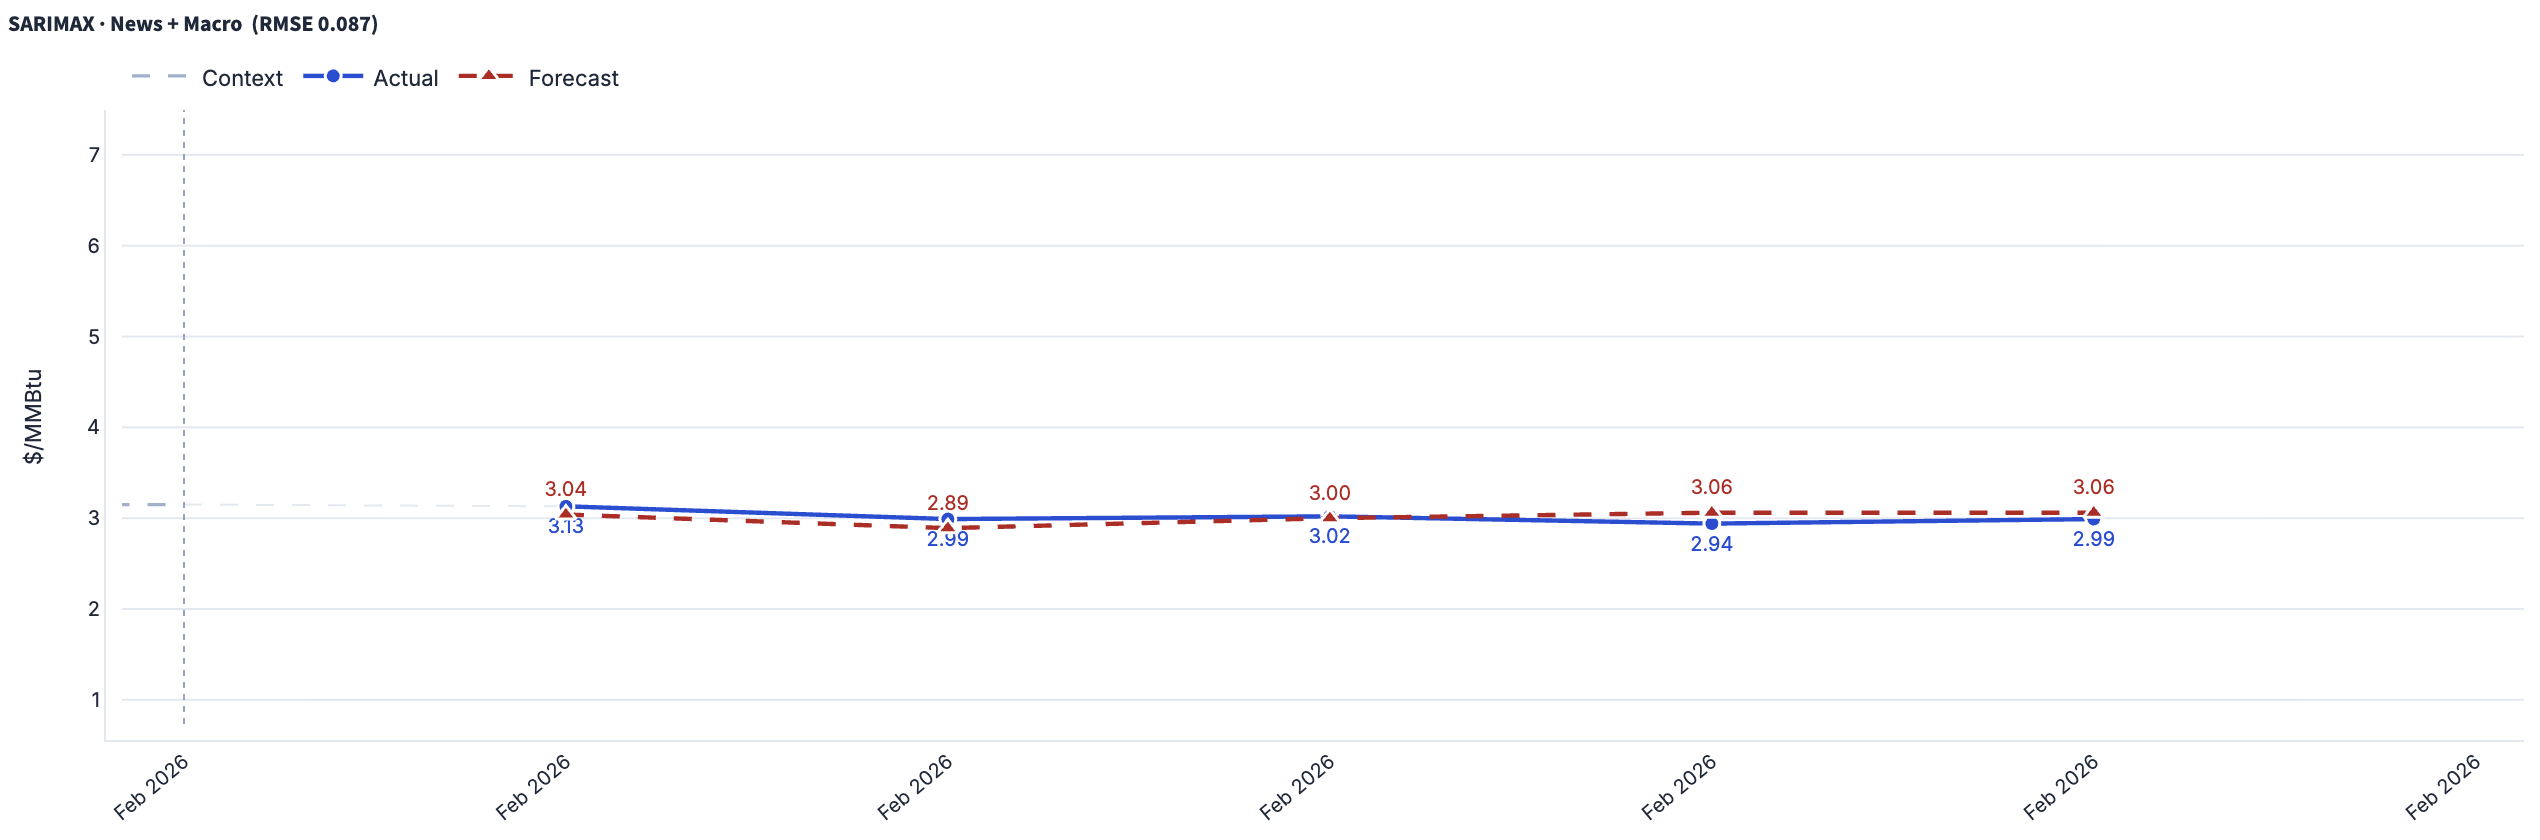
\includegraphics[width=\textwidth]{figures/multivariate_news_macro_cng_sarimax.png}
\small (a) SARIMAX forecast for natural gas
\end{minipage}\hfill
\begin{minipage}[t]{0.48\textwidth}
\centering
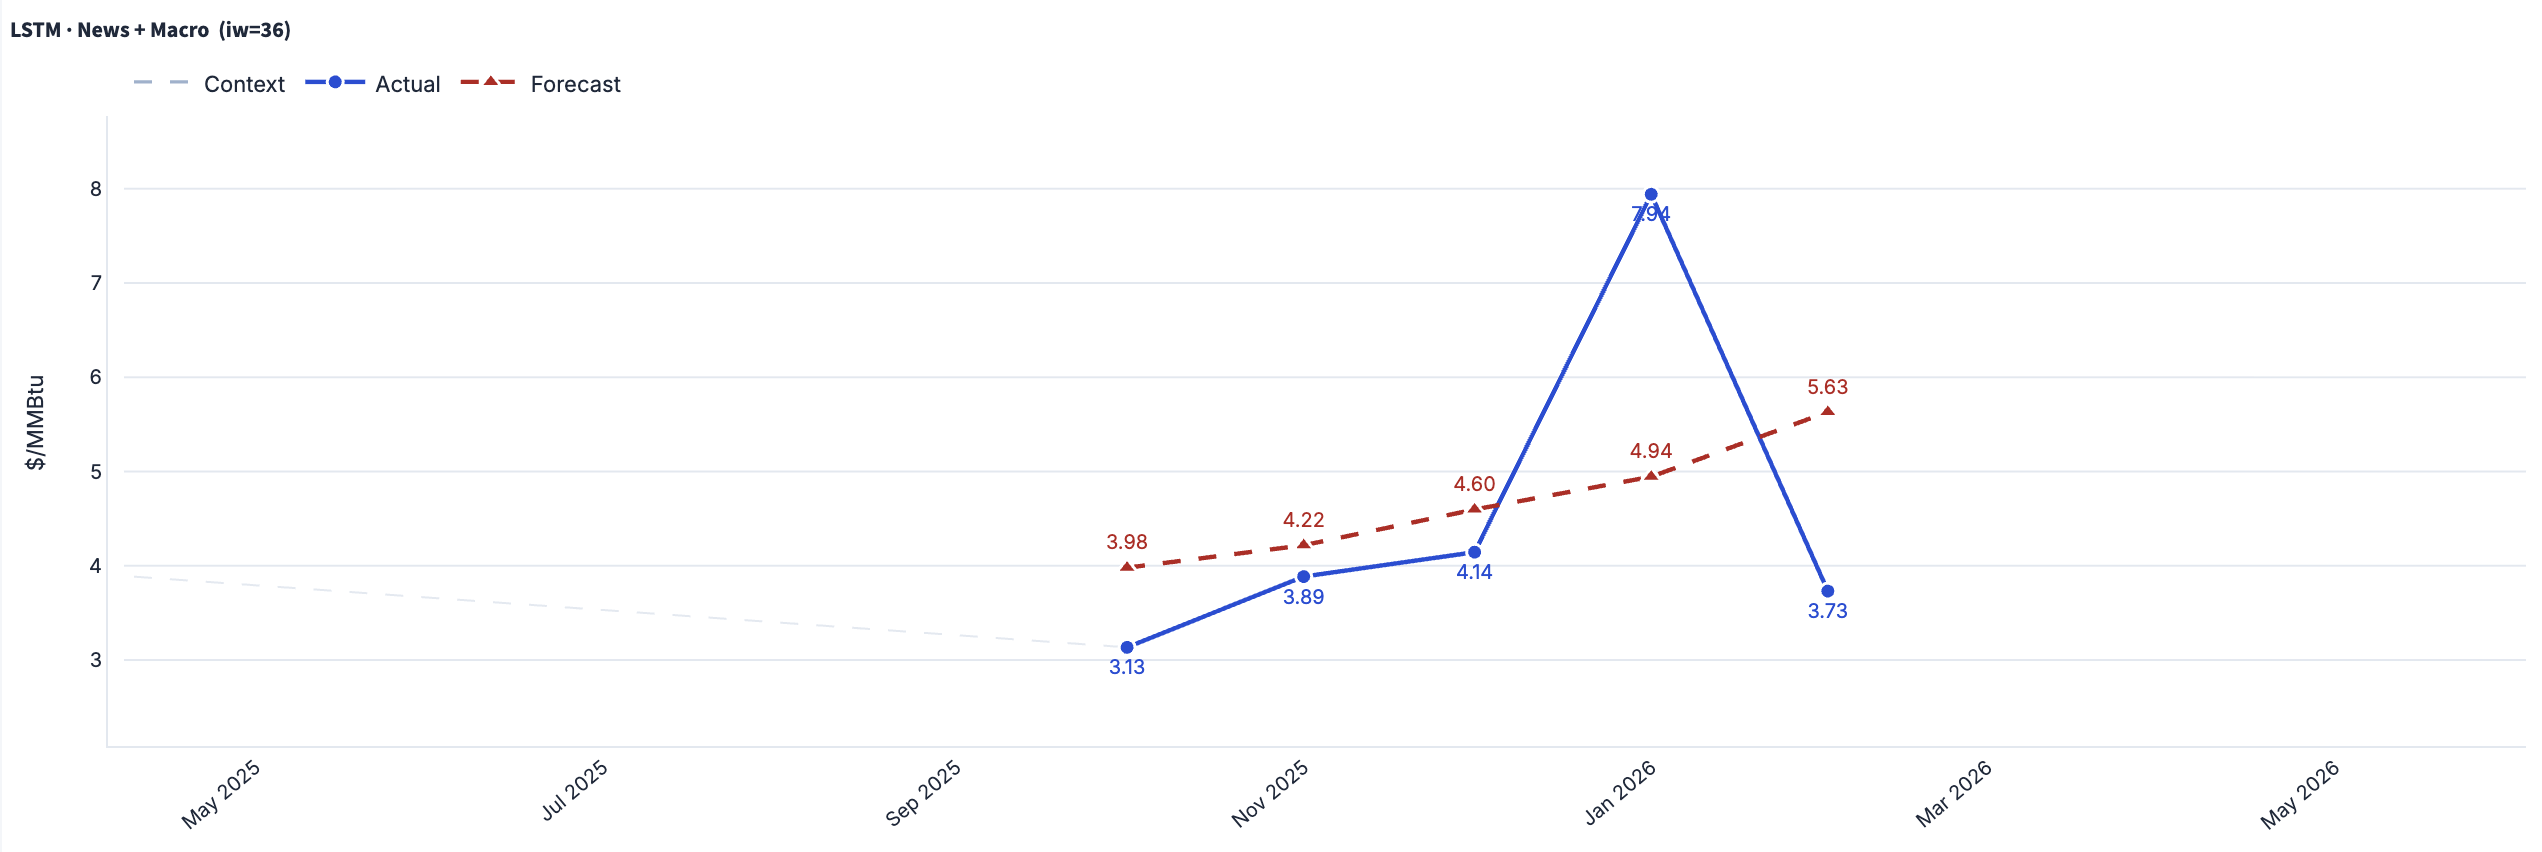
\includegraphics[width=\textwidth]{figures/multivariate_news_macro_cng_lstm.png}
\small (b) LSTM forecast for natural gas
\end{minipage}

\vspace{0.5em}

\begin{minipage}[t]{0.48\textwidth}
\centering
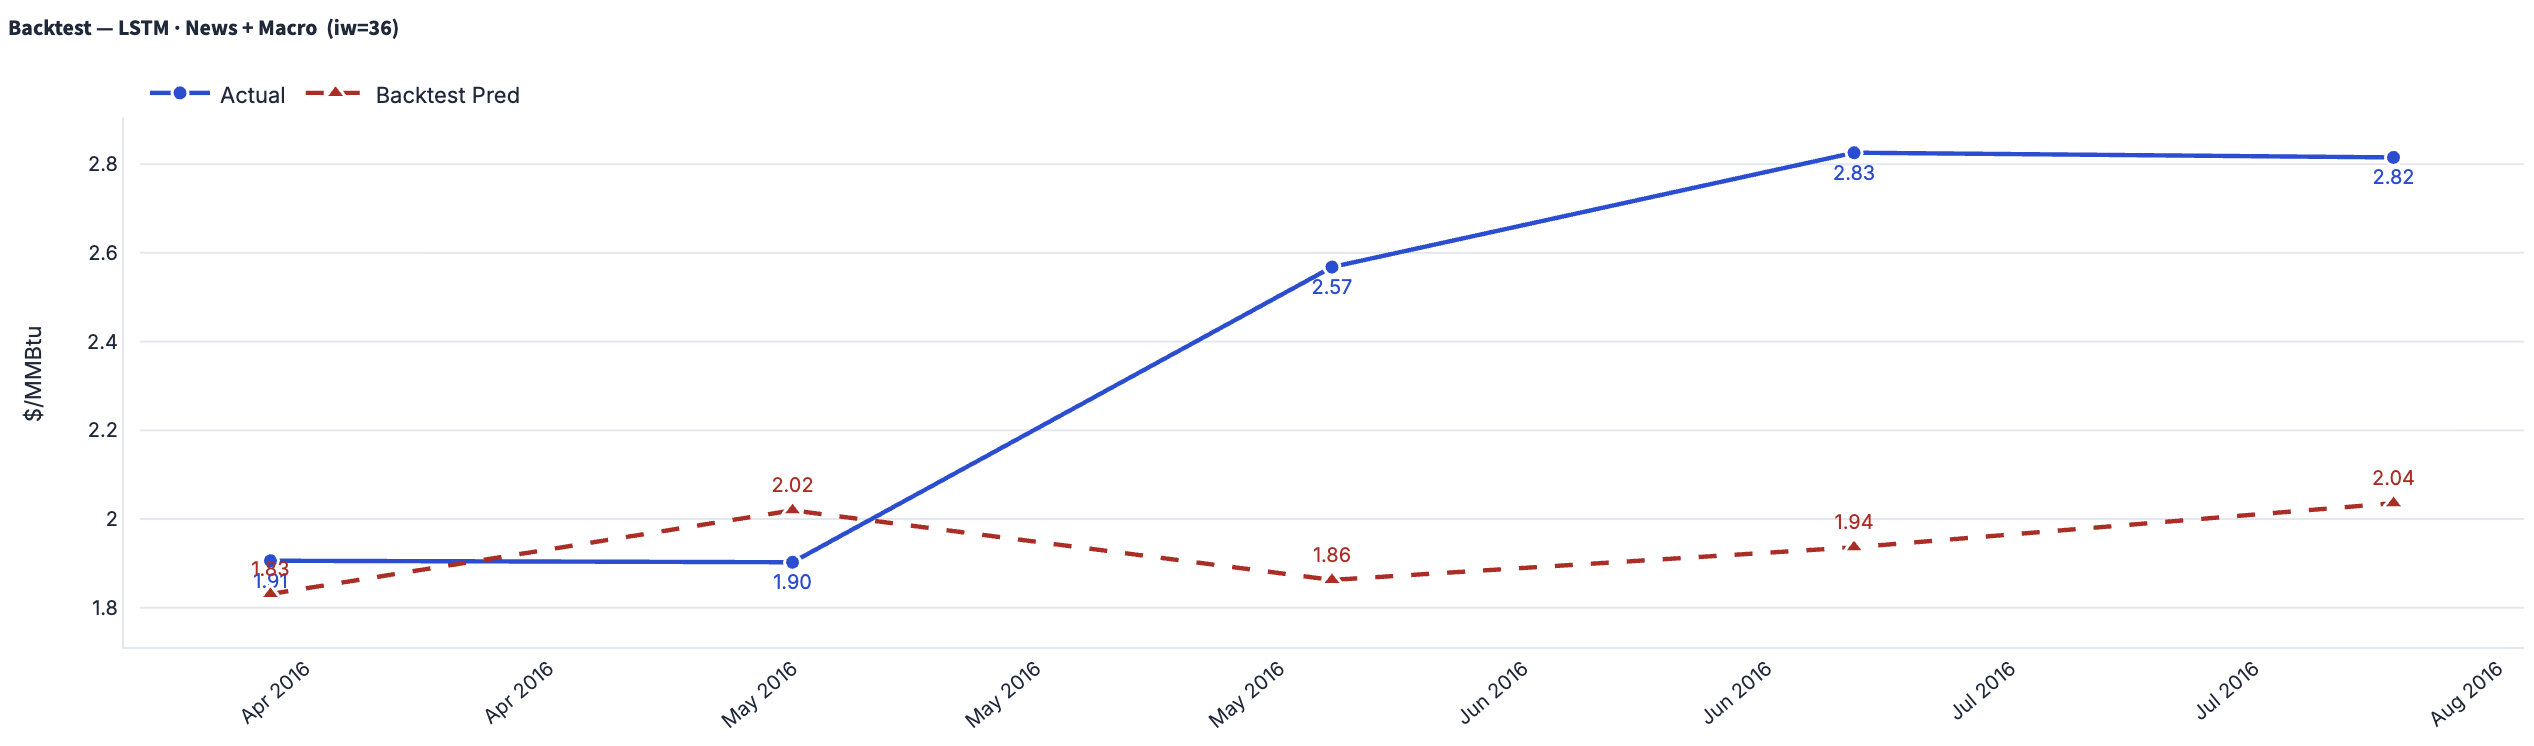
\includegraphics[width=\textwidth]{figures/multivariate_news_macro_cng_lstm_backtest.png}
\small (c) LSTM backtest for natural gas
\end{minipage}\hfill
\begin{minipage}[t]{0.48\textwidth}
\centering
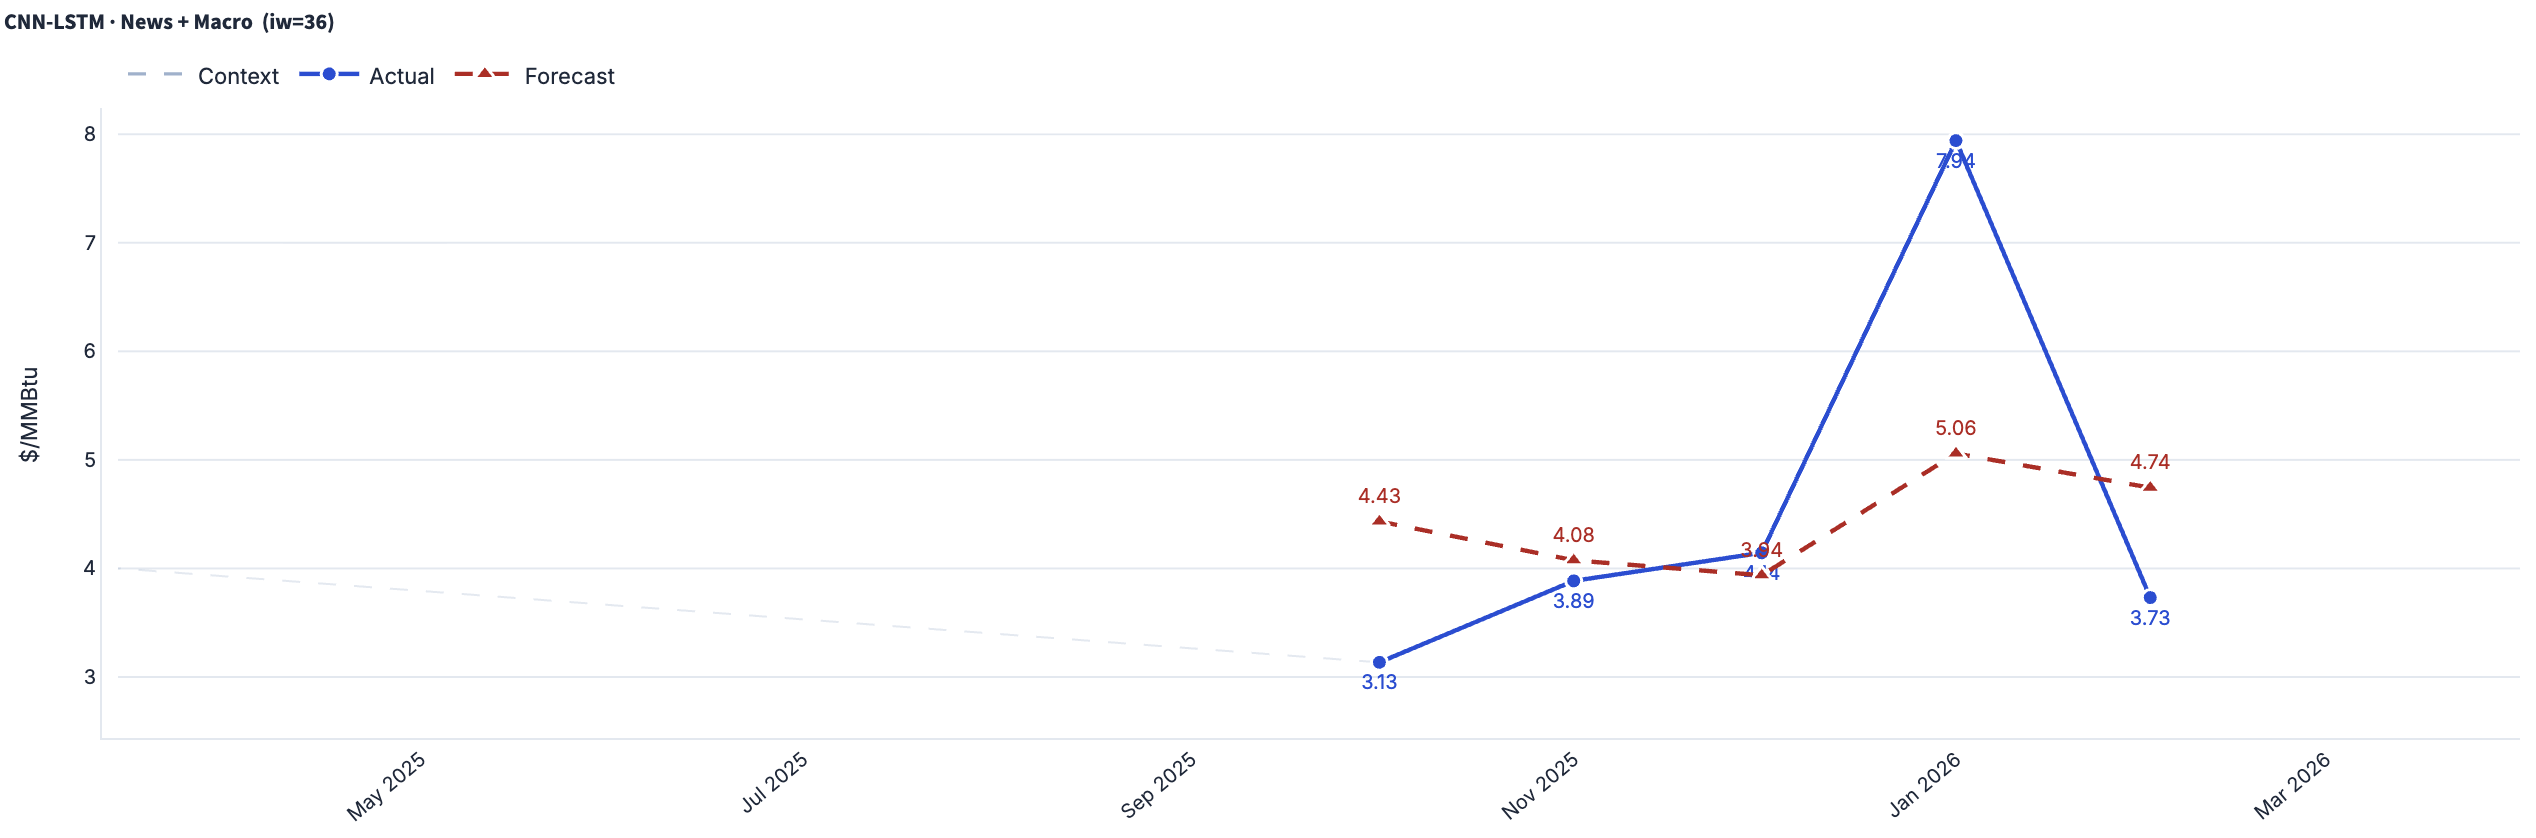
\includegraphics[width=\textwidth]{figures/multivariate_news_macro_cng_cnnlstm.png}
\small (d) CNN--LSTM forecast for natural gas
\end{minipage}

\vspace{0.5em}

\begin{minipage}[t]{0.48\textwidth}
\centering
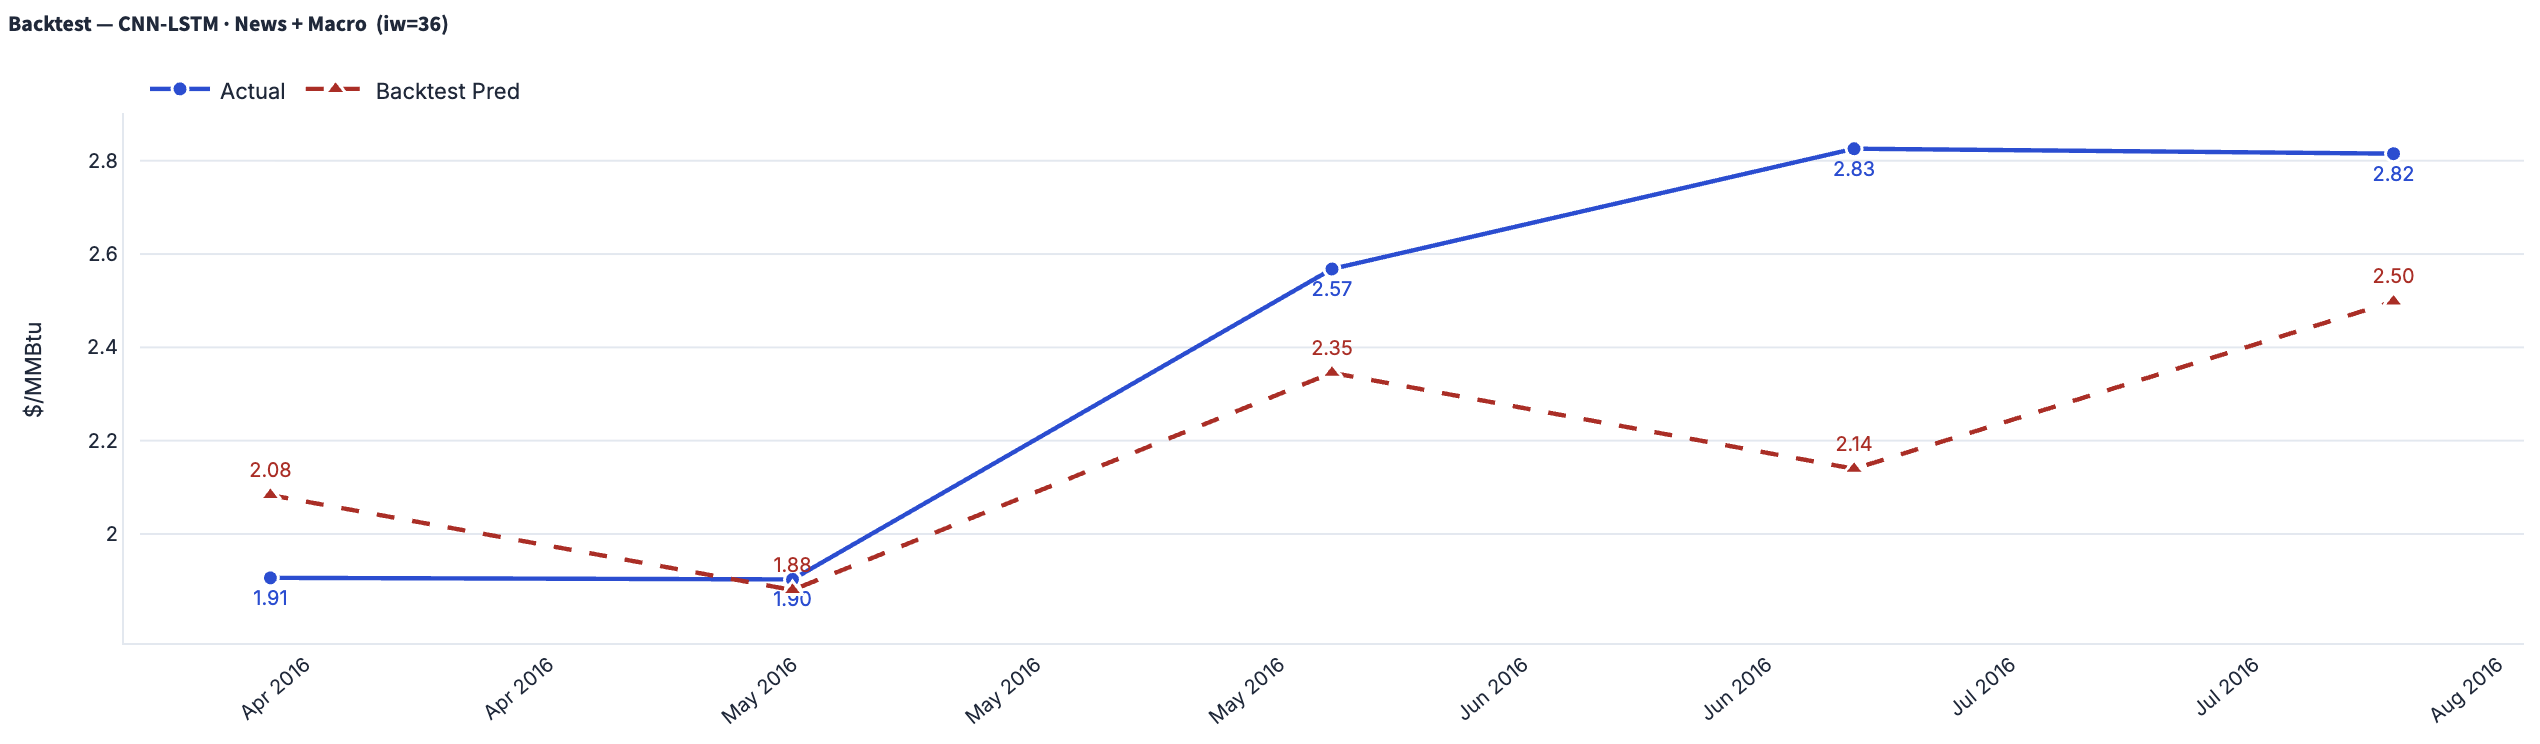
\includegraphics[width=\textwidth]{figures/multivariate_news_macro_cng_cnnlstm_backtest.png}
\small (e) CNN--LSTM backtest for natural gas
\end{minipage}
\caption{Actual versus predicted Henry Hub natural gas prices (USD/MMBtu) using the combined macroeconomic and GDELT-derived news feature set: (a) SARIMAX forecast, (b) LSTM direct forecast, (c) LSTM walk-forward backtest, (d) CNN--LSTM direct forecast, and (e) CNN--LSTM walk-forward backtest. This figure summarizes the joint-feature multivariate setting.}
\label{fig:combined_cng_plots}
\end{figure}

\begin{table}[h]
\centering
\caption{Combined macro-plus-news model performance for natural gas}
\label{tab:combined_cng}
\begin{tabular}{@{}lcccc@{}}
\toprule
Model & RMSE (USD/MMBtu) & MAE (USD/MMBtu) & MAPE (\%) & DA \\
\midrule
SARIMAX & 0.087 & 0.080 & 2.66 & 0.80 \\
LSTM Forecast & 1.650 & 1.305 & 27.01 & 0.40 \\
LSTM Backtest & 0.619 & 0.513 & 19.34 & 0.25 \\
CNN--LSTM Forecast & 1.490 & 1.118 & 22.95 & 0.60 \\
CNN--LSTM Backtest & 0.361 & 0.285 & 10.94 & 0.40 \\
\botrule
\end{tabular}
\end{table}

For natural gas, the combined setting shows comparatively lower error values than the macro-only and news-only setups. The SARIMAX results suggest that the joint feature space represents part of the variation in this series more effectively when macroeconomic and news-based inputs are used together. Compared with the earlier settings, the predictions in Figure~\ref{fig:combined_cng_plots} align more closely with the observed values, particularly in terms of direction and broad magnitude of change. This is reflected in the DA values as well, with SARIMAX reaching 0.80 and CNN--LSTM forecast reaching 0.60.

Unlike the crude-oil case, the neural models also show comparatively more consistent forecasting and backtesting behavior. This is especially visible for CNN--LSTM, whose backtest error for natural gas is lower than its corresponding crude-oil result, suggesting that the combined macro-plus-news inputs are relatively more useful for CNG in this architecture. Although the neural models remain less accurate than SARIMAX in absolute terms, they appear comparatively more stable here than in the isolated feature settings; even so, their DA values remain below the SARIMAX benchmark.

Taken together, the combined-model results suggest that integrating macroeconomic indicators with news-derived signals is comparatively more useful than using either source alone. The macro-only models struggled to track short-term variations, while the news-only models lacked stability and precision. By comparison, the combined models are more able to connect structured trends with event-driven information. SARIMAX shows the lowest errors in this setting, while the neural models, especially CNN--LSTM for CNG, also look comparatively better than in the separate feature settings, even though they still face challenges in reproducing extreme fluctuations.

For natural gas, the DM results remain non-significant even in the combined setting. The corresponding p-values are 0.190 for SARIMAX versus LSTM, 0.085 for SARIMAX versus CNN--LSTM, and 0.270 for LSTM versus CNN--LSTM. Hence, while the combined CNG models look numerically improved relative to the isolated feature settings, those gains should still be interpreted as suggestive rather than statistically conclusive.

\begin{table}[h]
\centering
\small
\caption{Best-performing model by setting and commodity}
\label{tab:summary_best_models}
\begin{tabular}{@{}p{1.5cm}p{1.8cm}p{0.8cm}p{1.8cm}p{0.7cm}p{3.8cm}@{}}
\toprule
Commodity & Lowest-RMSE Model & RMSE & Best-DA Model & DA & Interpretation \\
\midrule
Crude oil & SARIMAX & 1.235 & CNN--LSTM Forecast & 0.80 & In the combined setting, SARIMAX yields the lowest RMSE, whereas CNN--LSTM provides the strongest directional signal for crude oil. \\
Natural gas & SARIMAX & 0.087 & SARIMAX & 0.80 & In the combined setting, SARIMAX achieves both the lowest RMSE and the highest directional accuracy for natural gas. \\
\botrule
\end{tabular}
\end{table}

\section{Discussion}\label{sec12}

The experimental results reveal that predictive performance is strongly contingent on both the nature of the exogenous information incorporated and the commodity under examination - a finding that reflects the fundamentally different price formation processes governing crude oil and natural gas markets. In the macro-only setting, predictive performance remains uneven because broad economic indicators evolve more slowly than commodity prices and therefore explain medium-term conditions better than abrupt short-term moves. This structural mismatch between the low-frequency dynamics of macroeconomic variables and the higher-frequency movements of commodity prices helps explain why macro-only models can detect broad directional regime shifts while nonetheless failing to resolve the timing and magnitude of localized price shocks.

The news-only setting highlights a different trade-off. GDELT-based features contain relevant event information, but the aggregation process also introduces noise by compressing heterogeneous news into summary measures such as event counts, tone, and conflict intensity. As a result, news-only models can identify broad directional changes but often remain unstable, especially for natural gas, where sharp price movements are difficult to infer from aggregated event signals alone.

The combined macro-plus-news setting performs best because it brings together slower-moving structural context and faster-moving event-driven information. Economically, this means the models observe both the medium-horizon fundamentals that shape energy demand and financing conditions and the shorter-horizon news flow that signals geopolitical disruptions, policy uncertainty, and changes in market sentiment. In this setting, SARIMAX benefits most because many of the relevant transmission channels from macroeconomic conditions to monthly energy prices are comparatively stable and approximately linear over multi-year horizons. Variables such as industrial production, interest-rate conditions, exchange-rate movements, and aggregated news pressure can influence energy prices through demand strength, inventory expectations, trade competitiveness, and risk premia in ways that accumulate gradually rather than instantaneously. Once these economically meaningful inputs are present, SARIMAX can map them efficiently into price dynamics while preserving the autoregressive and seasonal structure of the series.

By contrast, LSTM and CNN--LSTM offer greater representational flexibility, but that flexibility is not automatically advantageous in this empirical setting. The available sample is modest relative to the parameterization needs of neural architectures, the data frequency is monthly rather than high-frequency, and the exogenous features are already aggregated into relatively smooth summary indicators. Economically, this reduces the scope for rich nonlinear interactions that deep models are designed to exploit. Instead of uncovering additional market structure, the neural models may overemphasize local fluctuations or learn overly smoothed relationships, which can weaken their response to abrupt commodity-price revaluations. Thus, when the joint feature space is sufficiently informative, the superior performance of SARIMAX likely reflects the fact that medium-run energy pricing is still anchored by interpretable macroeconomic fundamentals and persistent event-driven pressures that linear dynamic models are well suited to capture.

Overall, the findings suggest that exogenous variables are most valuable as complementary signals rather than as isolated substitutes for price history. Relative to prior work that typically studies one commodity, one model family, or one exogenous source at a time, this comparison shows more clearly where macroeconomic and news-based inputs appear useful and where their effects remain limited. Their main value in this study is not perfect point forecasting, but improved directional understanding, better turning-point detection, and a more interpretable view of which external conditions coincide with changing energy prices.

\section{Limitations and Future Work}\label{sec14}

Energy price forecasting remains challenging due to the complex interplay of economic, geopolitical, and market-specific factors, many of which are not fully represented by the selected macroeconomic indicators and aggregated news signals. While these inputs provide useful context, they may fail to represent sudden shocks or localized events that drive sharp price movements. Additionally, classical time series models are inherently linear and may not fully model nonlinear relationships, while neural network models, although more flexible, tend to produce smoother outputs and may struggle to respond to high volatility and abrupt changes in the data.

A further limitation pertains to the representational granularity of the news data. The use of aggregated GDELT features improves computational efficiency but reduces the granularity of event-level information, potentially limiting the richness of extracted signals. Furthermore, the inherent noise and variability in energy price series, particularly in natural gas markets, can affect model stability and generalization across different time periods, leading to inconsistent performance under different conditions.

Future work can address these limitations by expanding both the feature space and modeling strategies. This includes testing models with additional macroeconomic variables that are indirectly correlated with energy prices, which may reflect hidden economic influences. Future work could substantially improve the quality and specificity of news-based signals by replacing aggregated GDELT summary statistics with richer natural language representations - such as transformer-derived sentence embeddings (e.g., BERT, FinBERT) - applied directly to the source text of relevant news articles. Further, modeling the temporal impact of events, including how long a news event influences prices through temporal weighting mechanisms, can provide deeper insight into market behavior. Finally, exploring more advanced architectures, such as attention-based or transformer models, may improve the ability to model complex dependencies and enhance overall forecasting performance.


\section{Conclusion}\label{sec13}

This study investigated the extent to which macroeconomic indicators sourced from the FRED database and event-driven news signals derived from the GDELT repository can appreciably improve the forecasting accuracy and directional tracking of WTI crude oil and Henry Hub natural gas prices. The empirical results show that both sources of information are helpful, especially when we use them together within a multivariate framework. Across the experiments, the combined macro-plus-news setting consistently outperformed the macro-only and news-only alternatives, indicating that structured economic signals and event-driven information reflect complementary aspects of energy price behavior.

The findings also suggest that GDELT-based features and macroeconomic variables are informative for detecting broad market direction and relevant shifts in oil and gas prices, even when the models are not always able to track future fluctuations with high precision. In particular, the combined-feature SARIMAX models delivered the most reliable overall performance, suggesting that the joint feature space introduces substantive explanatory relationships that are not visible in isolated settings. Economically, this indicates that monthly oil and gas prices continue to co-move with a set of relatively persistent macro-financial fundamentals, while aggregated news signals add timely information about changing market stress and event risk. Neural architectures such as LSTM and CNN--LSTM were also able to model parts of the underlying dynamics, but their forecasting and backtesting performance remained less stable, especially during periods of abrupt price change, implying that the nonlinear structure present in these inputs was not strong enough or not measured finely enough to offset the advantages of a more disciplined linear dynamic specification.

Taken together, the empirical results indicate that the incorporation of heterogeneous exogenous information materially improves directional energy price modeling and reduces forecast error in well-specified linear frameworks, while simultaneously confirming that precise short-term point forecasting of volatile commodity prices remains an open and non-trivial research problem. Energy markets are influenced by rapidly changing geopolitical events, structural breaks, and nonlinear interactions that are not fully represented by aggregated macroeconomic indicators or news summaries alone. For this reason, the proposed framework should be viewed as a notable step toward richer predictive modeling rather than a complete solution to the forecasting problem.

From a research perspective, this study contributes a comparative framework for evaluating univariate and multivariate models under a consistent validation setting, while also demonstrating the practical value of combining structured macroeconomic variables with event-driven news features. The results are particularly important because they show that external signals can improve directional understanding and reduce error substantially, even when exact point forecasting remains challenging.

%%===========================================================================================%%
%% References included directly in the manuscript file                                      %%
%%===========================================================================================%%

\begin{thebibliography}{28}

\bibitem{akaike1974}
Akaike, H.: A new look at the statistical model identification. IEEE Transactions on Automatic Control \textbf{19}(6), 716--723 (1974).

\bibitem{akiba2019optuna}
Akiba, T., Sano, S., Yanase, T., Ohta, T., Koyama, M.: Optuna: A next-generation hyperparameter optimization framework. In: Proceedings of the 25th ACM SIGKDD International Conference on Knowledge Discovery and Data Mining, pp. 2623--2631 (2019).

\bibitem{baker2016}
Baker, S.R., Bloom, N., Davis, S.J.: Measuring economic policy uncertainty. The Quarterly Journal of Economics \textbf{131}(4), 1593--1636 (2016).

\bibitem{baumeister2016}
Baumeister, C., Kilian, L.: Forty years of oil price fluctuations: why the price of oil may still surprise us. Journal of Economic Perspectives \textbf{30}(1), 139--160 (2016).

\bibitem{box1976}
Box, G.E.P., Jenkins, G.M.: \textit{Time Series Analysis: Forecasting and Control}. Holden-Day, San Francisco (1976).

\bibitem{busari2021}
Busari, G.A., Lim, D.H.: Crude oil price prediction: a comparison between AdaBoost-LSTM and AdaBoost-GRU for improving forecasting performance. Computers \& Chemical Engineering \textbf{155}, 107513 (2021).

\bibitem{cen2019}
Cen, Z., Wang, J.: Crude oil price prediction model with long short-term memory deep learning based on prior knowledge data transfer. Energy \textbf{169}, 160--171 (2019).

\bibitem{dickey1979}
Dickey, D.A., Fuller, W.A.: Distribution of the estimators for autoregressive time series with a unit root. Journal of the American Statistical Association \textbf{74}(366), 427--431 (1979).

\bibitem{diebold1995}
Diebold, F.X., Mariano, R.S.: Comparing predictive accuracy. Journal of Business \& Economic Statistics \textbf{13}(3), 253--263 (1995).

\bibitem{durbin2012}
Durbin, J., Koopman, S.J.: \textit{Time Series Analysis by State Space Methods}, 2nd edn. Oxford University Press, Oxford (2012).

\bibitem{fred2025}
Federal Reserve Bank of St. Louis: Federal Reserve Economic Data (FRED). \url{https://fred.stlouisfed.org/} (accessed 2025).

\bibitem{gers2000}
Gers, F.A., Schmidhuber, J., Cummins, F.: Learning to forget: continual prediction with LSTM. Neural Computation \textbf{12}(10), 2451--2471 (2000).

\bibitem{goldstein1992}
Goldstein, J.S.: A conflict-cooperation scale for WEIS events data. Journal of Conflict Resolution \textbf{36}(2), 369--385 (1992).

\bibitem{hamilton2003}
Hamilton, J.D.: What is an oil shock? Journal of Econometrics \textbf{113}(2), 363--398 (2003).

\bibitem{hamilton2009}
Hamilton, J.D.: Causes and consequences of the oil shock of 2007--08. Brookings Papers on Economic Activity \textbf{2009}(1), 215--261 (2009).

\bibitem{hochreiter1997}
Hochreiter, S., Schmidhuber, J.: Long short-term memory. Neural Computation \textbf{9}(8), 1735--1780 (1997).

\bibitem{huber1964}
Huber, P.J.: Robust estimation of a location parameter. Annals of Mathematical Statistics \textbf{35}(1), 73--101 (1964).

\bibitem{hyndman2018}
Hyndman, R.J., Athanasopoulos, G.: \textit{Forecasting: Principles and Practice}, 2nd edn. OTexts, Melbourne (2018).

\bibitem{kilian2009}
Kilian, L.: Not all oil price shocks are alike: disentangling demand and supply shocks in the crude oil market. American Economic Review \textbf{99}(3), 1053--1069 (2009).

\bibitem{kim2018}
Kim, H.Y., Won, C.H.: Forecasting the volatility of stock price index: a hybrid model integrating LSTM with multiple GARCH-type models. Expert Systems with Applications \textbf{103}, 25--37 (2018).

\bibitem{kingma2015}
Kingma, D.P., Ba, J.: Adam: a method for stochastic optimization. In: International Conference on Learning Representations (2015).

\bibitem{kwiatkowski1992}
Kwiatkowski, D., Phillips, P.C.B., Schmidt, P., Shin, Y.: Testing the null hypothesis of stationarity against the alternative of a unit root. Journal of Econometrics \textbf{54}(1--3), 159--178 (1992).

\bibitem{lecun1998}
LeCun, Y., Bottou, L., Bengio, Y., Haffner, P.: Gradient-based learning applied to document recognition. Proceedings of the IEEE \textbf{86}(11), 2278--2324 (1998).

\bibitem{leetaru2013}
Leetaru, K., Schrodt, P.A.: GDELT: Global Data on Events, Location, and Tone, 1979--2012. In: ISA Annual Convention (2013).

\bibitem{li2014}
Li, X., Xie, H., Chen, L., Wang, J., Deng, X.: News impact on stock price return via sentiment analysis. Knowledge-Based Systems \textbf{69}, 14--23 (2014).

\bibitem{sainath2015}
Sainath, T.N., Vinyals, O., Senior, A., Sak, H.: Convolutional, long short-term memory, fully connected deep neural networks. In: Proceedings of the IEEE International Conference on Acoustics, Speech and Signal Processing (ICASSP), pp. 4580--4584 (2015).

\bibitem{shapiro2022}
Shapiro, A.H., Sudhof, M., Wilson, D.J.: Measuring news sentiment. Journal of Econometrics \textbf{228}(2), 221--243 (2022).

\bibitem{tetlock2007}
Tetlock, P.C.: Giving content to investor sentiment: the role of media in the stock market. The Journal of Finance \textbf{62}(3), 1139--1168 (2007).

\end{thebibliography}

\end{document}

\subsubsection{GDELT Data Processing}\label{subsubsec:gdeltprocessing}

We process the GDELT dataset to extract substantive signals from large-scale event data. The preprocessing steps include filtering the dataset to retain only US-related events, treating `EventCode' as a categorical variable with one-hot encoding, aggregating event counts on a daily basis, and computing summary statistics such as average Goldstein Scale and average tone. When required, we further aggregate the data to the monthly level. This approach reduces millions of raw records into a compact and interpretable time series representation of global events.

\subsubsection{Data Integration}\label{subsubsec:dataintegration}

The processed macroeconomic and GDELT datasets are merged using a common date index. Only the overlapping time period between the datasets is retained to ensure consistency. This step helps eliminate missing value issues and ensures that all features are temporally aligned for modeling.

\subsection{Data Splitting Strategy}\label{subsec:datasplitting}

We use different data-splitting strategies for classical and neural network-based models to ensure fair and reliable evaluation. For classical time-series models, we divide the dataset into training and testing sets. This setup evaluates each model's ability to forecast near-future values from past trends.

\begin{table}[h]
\centering
\caption{Classical model data splitting}
\label{tab:classical_data_split}
\begin{tabular}{@{}lll@{}}
\toprule
Stage & Sequence Range & Role \\
\midrule
Train & January 2014--October 2025 & Model estimation \\
Test & November 2025--March 2026 & Final held-out evaluation \\
\botrule
\end{tabular}
\end{table}

Neural network-based models follow a more structured approach involving backtest, train, and test segments. Backtesting is particularly important to verify that the model learns non-trivial temporal patterns rather than fitting random noise. To keep the split rule uniform across neural configurations, we define the blocks using the input-window size alone. Specifically, for an input window of size $k$, the backtest segment spans indices $0$ through $k+5$, and the held-out test segment spans indices $n-(k+5)$ through $n$. We use the observations between these two segments for training. Table~\ref{tab:data_split_strategy} summarizes this ordering.

\begin{table}[h]
\caption{Data splitting and sliding window strategy}\label{tab:data_split_strategy}
\begin{tabular}{@{}lllll@{}}
\toprule
Stage & Calendar Order & Sequence Definition & Role \\
\midrule
Backtest & First & $0 \rightarrow k+5$ & Rolling validation \\
Train & Second & $(k+6) \rightarrow n-(k+6)$ & Model fitting \\
Test & Final & $n-(k+5) \rightarrow n$ & Held-out evaluation \\
\botrule
\end{tabular}
\end{table}

After integrating the FRED and GDELT sources, the retained monthly sample spans January 2014 through March 2026. For the neural-network models, the split is determined only by input-window size. Accordingly, the backtest block occupies the first $k+5$ months, the test block occupies the last $k+5$ months, and we use the remaining middle segment for training.

\begin{table}[h]
\centering
\caption{Exact calendar ranges used for neural-network train, test, and backtest splits}
\label{tab:exact_split_dates}
\begin{tabular}{@{}llll@{}}
\toprule
Input Window Size & Backtest & Train & Test \\
\midrule
$5$ & Jan 2014--Oct 2014 & Nov 2014--May 2025 & Jun 2025--Mar 2026 \\
$10$ & Jan 2014--Mar 2015 & Apr 2015--Dec 2024 & Jan 2025--Mar 2026 \\
$24$ & Jan 2014--May 2016 & Jun 2016--Oct 2023 & Nov 2023--Mar 2026 \\
$36$ & Jan 2014--May 2017 & Jun 2017--Oct 2022 & Nov 2022--Mar 2026 \\
\botrule
\end{tabular}
\end{table}
\subsection{Key Design Principles}\label{subsec:keydesign}

The pipeline is guided by a set of key design principles. Strict adherence to temporal ordering is enforced at every stage of the pipeline to preserve the causal structure of the time series and to prevent any form of look-ahead bias that would artificially inflate model performance. In accordance with the no-future-information constraint fundamental to
out-of-sample forecasting evaluation, all models are trained exclusively on
observations preceding the forecast horizon, with strict enforcement applied
across both the classical and neural network model classes. Additionally, data leakage is carefully prevented across all stages of the pipeline. Finally, a consistent preprocessing strategy is applied across both classical and neural models, enabling fair comparison and reliable evaluation.


Overall, this preprocessing and data preparation pipeline ensures reliable integration of macroeconomic indicators and news-based signals. It provides a strong foundation for comparing different forecasting models while maintaining interpretability and robustness in the analysis.

\subsection{Stationarity Testing}\label{subsec:stationarity}

We perform stationarity testing before fitting the classical time-series models in order to determine whether the mean and variance structure of each series remains sufficiently stable over time for ARIMA-type modeling. In particular, we use both the Augmented Dickey--Fuller (ADF) test and the Kwiatkowski--Phillips--Schmidt--Shin (KPSS) test to assess stationarity. The ADF test evaluates the null hypothesis $H_0$, that the series contains a unit root and is therefore non-stationary, against the alternative hypothesis $H_1$, that the series does not contain a unit root and is stationary. Equivalently, in the regression specification below, these hypotheses correspond to $H_0: \phi = 0$ versus $H_1: \phi < 0$. By contrast, the KPSS test adopts stationarity as the null hypothesis and non-stationarity as the alternative. A significance level of $\alpha = 0.05$ is used throughout, so the null hypothesis is rejected when the corresponding test $p$-value is less than 0.05. In this study, stationarity is therefore checked using both ADF and KPSS before model fitting. The ADF regression is given by
\begin{equation}
 \Delta y_t = \alpha + \beta t + \phi y_{t-1} + \sum_{i=1}^{p} \gamma_i \Delta y_{t-i} + \epsilon_t,
\label{eq:adf}
\end{equation}
The KPSS test statistic is computed as
\begin{equation}
 \mathrm{KPSS} = \frac{1}{T^2 \hat{\sigma}^2} \sum_{t=1}^{T} S_t^2,
\label{eq:kpss}
\end{equation}
where $S_t = \sum_{i=1}^{t} e_i$ denotes the cumulative partial sum of the residuals from the regression used in the KPSS procedure, $T$ is the sample size, and $\hat{\sigma}^2$ is the long-run variance estimate of the residual process. In the ADF regression above, $\alpha$ is a constant, $\beta t$ is a deterministic trend component, $\phi$ is the coefficient on the lagged level term $y_{t-1}$ and is the key parameter used to assess the presence of a unit root, $p$ is the lag order selected using an information criterion such as AIC or BIC, and $\epsilon_t$ is a white-noise error term. When the ADF null hypothesis cannot be rejected or the KPSS null hypothesis is rejected, the series is differenced and re-evaluated until stationarity is achieved. The number of differences required to obtain stationarity determines the integration order $d$ used in the corresponding ARIMA$(p,d,q)$ specification. In the empirical preprocessing stage, the level series generally did not satisfy the combined stationarity criteria, but the transformed series used for classical modeling satisfied both the ADF and KPSS tests at the 5\% significance level after the required differencing step, indicating that the final modeling inputs were stationary.

\subsection{Modeling}\label{subsec:modeling}

This study employs both classical statistical models and neural network-based approaches to represent different characteristics of energy price data. Classical models are used as a baseline due to their simplicity and interpretability, while neural network models are explored to model nonlinear relationships, interactions among variables, and temporal dependencies present in multivariate time series.

\subsubsection*{4.4.1 Classical Modeling}\label{subsubsec:classicalmodeling}

\subsubsection*{4.4.1.1 ARIMA}

In ARIMA, the model first transforms the time series into a stationary form through differencing. Then, for each time step $t$, the model computes the predicted value by combining a weighted sum of previous observations and previous error terms, as defined by,
\begin{equation}
 y_t = c + \sum_{i=1}^{p} \phi_i y_{t-i} + \sum_{j=1}^{q} \theta_j \epsilon_{t-j} + \epsilon_t.
\label{eq:arima}
\end{equation}
Here, the algorithm iteratively learns coefficients $\phi_i$ and $\theta_j$, which determine how much influence past values and past errors have on the current prediction. This makes ARIMA effective for modeling linear temporal dependencies in univariate data.

\subsubsection*{4.4.1.2 SARIMA}

SARIMA follows the same process as ARIMA but extends it by incorporating seasonal patterns. After differencing both regular and seasonal components, the model applies seasonal autoregressive and moving average terms:
\begin{equation}
 \Phi_P(B^s)\phi_p(B)(1-B)^d(1-B^s)^D y_t = \Theta_Q(B^s)\theta_q(B)\epsilon_t.
\label{eq:sarima}
\end{equation}
In this formulation, the algorithm represents repeating cycles by applying operations at lag intervals defined by the seasonal period $s$. This allows the model to account for periodic fluctuations observed in energy price data.

\subsubsection*{4.4.1.3 SARIMAX}

SARIMAX extends SARIMA by integrating external variables into the prediction step. At each time step, the model not only considers past values and errors but also includes the contribution from exogenous variables:
\begin{equation}
 y_t = c + \sum_{i=1}^{p} \phi_i y_{t-i} + \sum_{j=1}^{q} \theta_j \epsilon_{t-j} + \beta X_t + \epsilon_t.
\label{eq:sarimax}
\end{equation}
Here, the algorithm learns an additional set of coefficients $\beta$ that quantify the influence of macroeconomic and news-based features $X_t$. This enables the model to incorporate real-world drivers of price movement, making it more suitable for multivariate forecasting.

\subsubsection*{4.4.2 Neural Network-Based Modeling}\label{subsubsec:neuralmodeling}

Neural network models learn patterns directly from data by optimizing weights through iterative training. Instead of explicitly defining relationships, they approximate complex mappings between input sequences and outputs.

\subsubsection*{4.4.2.1 LSTM}

In LSTM, the model processes the input sequence step by step, where each input $x_t$ and previous hidden state $h_{t-1}$ are used to update the memory cell. At each step, the algorithm computes gate values to control information flow:
\begin{align}
 f_t &= \sigma\left(W_f[h_{t-1}, x_t] + b_f\right), \nonumber \\
 i_t &= \sigma\left(W_i[h_{t-1}, x_t] + b_i\right), \nonumber \\
 \tilde{C}_t &= \tanh\left(W_c[h_{t-1}, x_t] + b_c\right).
\label{eq:lstm_gates}
\end{align}
The cell state is then updated as
\begin{equation}
 C_t = f_t \cdot C_{t-1} + i_t \cdot \tilde{C}_t,
\label{eq:lstm_cell}
\end{equation}
and the hidden state is computed as
\begin{equation}
 h_t = o_t \cdot \tanh(C_t).
\label{eq:lstm_hidden}
\end{equation}
This step-by-step process allows the model to selectively retain or forget information across time steps. Finally, the last hidden state is passed through a linear layer,
\begin{equation}
 \hat{y} = W h_t + b,
\label{eq:lstm_output}
\end{equation}
to generate the forecast output. This mechanism enables LSTM to model long-term dependencies in sequential data. In implementation, the LSTM receives input tensors of shape $(\text{batch}, \text{time}, \text{features})$ and maps the final hidden representation to a continuous forecast through a linear output layer, making it suitable for nonlinear multivariate sequence learning.

\subsubsection*{4.4.2.2 CNN--LSTM}

The CNN--LSTM model follows a two-stage process. First, the input sequence is passed through a convolutional layer,
\begin{equation}
 z = \mathrm{Conv1D}(x),
\label{eq:conv1d}
\end{equation}
which extracts local temporal features by applying filters across time steps. This transforms the input into feature maps that highlight short-term patterns.Next, these extracted features are passed into the LSTM layer,
\begin{equation}
 h_t = \mathrm{LSTM}(z_t),
\label{eq:cnn_lstm}
\end{equation}
where the LSTM processes the sequence of feature maps to model long-term dependencies. Finally, the output is computed using
\begin{equation}
 \hat{y} = W h_t + b.
\label{eq:cnn_lstm_output}
\end{equation}
This combination allows the model to first identify local structures and then learn their evolution over time, making it particularly effective for complex time series influenced by multiple factors. As with the LSTM, the CNN--LSTM operates on tensors of shape $(\text{batch}, \text{time}, \text{features})$, with the final recurrent representation passed to a linear layer for continuous-value prediction.

\subsubsection*{4.4.3 Hyperparameter Tuning}\label{subsubsec:hypertuning}

To improve model performance, hyperparameters are optimized using Optuna. The tuning process iteratively evaluates different configurations by adjusting parameters such as sequence length, number of LSTM units, convolution filters, kernel size, dropout rate, learning rate, and batch size. This search process ensures that both LSTM and CNN--LSTM models are trained under optimal settings across different feature combinations, including univariate, macro-only, news-only, and combined inputs. For each configuration, Optuna is run for 30 trials and the neural models are trained with batch size set to 32. Optimization uses Adam with Huber loss, which is more robust to extreme forecast errors than mean squared error, and early stopping is applied on validation loss to reduce overfitting and retain the best-performing weights.

\subsubsection*{4.4.4 Evaluation and Backtesting}\label{subsubsec:evaluation}

We evaluate model performance using three standard error measures: Root Mean Squared Error (RMSE), Mean Absolute Error (MAE), and Mean Absolute Percentage Error (MAPE). RMSE penalizes large errors more strongly and is useful when large forecast deviations are especially undesirable. MAE provides an interpretable average magnitude of the forecast error. MAPE expresses the error in percentage terms, which helps compare model performance across crude oil and natural gas despite their different price scales.

The metrics are defined as follows:
\begin{equation}
\mathrm{RMSE} = \sqrt{\frac{1}{n}\sum_{t=1}^{n}(y_t - \hat{y}_t)^2},
\label{eq:rmse}
\end{equation}
\begin{equation}
\mathrm{MAE} = \frac{1}{n}\sum_{t=1}^{n}\left|y_t - \hat{y}_t\right|,
\label{eq:mae}
\end{equation}
\begin{equation}
\mathrm{MAPE} = \frac{100}{n}\sum_{t=1}^{n}\left|\frac{y_t - \hat{y}_t}{y_t}\right|.
\label{eq:mape}
\end{equation}
To assess whether observed differences in forecast accuracy between model pairs are statistically significant rather than attributable to sampling variability, the Diebold--Mariano (DM) test~\cite{diebold1995} is applied. Let the loss differential be defined as
\begin{equation}
 d_t = L(e_{1t}) - L(e_{2t}),
\label{eq:dm_loss}
\end{equation}
where $L(\cdot)$ is a loss function and, in this study, squared error is used. The DM statistic is then given by
\begin{equation}
\mathrm{DM} = \frac{\bar{d}}{\sqrt{\hat{V}(\bar{d})/n}} \sim \mathcal{N}(0,1),
\label{eq:dm_stat}
\end{equation}
under the null hypothesis of equal predictive accuracy. Rejection of $H_0$ at the 5\% level ($p < 0.05$) provides formal statistical evidence that one model forecasts significantly better than another.

To formally evaluate directional forecasting capability --- a practically important property in commodity price applications --- we also compute Directional Accuracy (DA):
\begin{equation}
\mathrm{DA} = \frac{1}{n}\sum_{t=1}^{n} \mathbb{1}\left[(y_t - y_{t-1})(\hat{y}_t - y_{t-1}) > 0\right].
\label{eq:da}
\end{equation}
Here, $y_t$ denotes the observed value at time $t$, $\hat{y}_t$ denotes the predicted value, and $n$ is the number of forecast points in the evaluation sample.

In Equation~\ref{eq:da}, $\mathbb{1}[\cdot]$ is the indicator function, which takes value 1 when the predicted and actual price changes share the same sign and 0 otherwise. A value of $\mathrm{DA}=0.5$ is equivalent to a random directional guess, whereas values substantially above 0.5 indicate genuine directional predictive skill.

Accordingly, the results tables in Section~\ref{sec5} report DA alongside RMSE, MAE, and MAPE so that point forecast accuracy and directional performance can be interpreted jointly.

In addition to test-set forecasting, we use backtesting to assess temporal robustness. In this study, backtesting means that we repeatedly train the model only on past data and then test it on later observations that were not seen during training. At each step, the training window contains historical observations up to a given time point, and we evaluate the model on the next unseen segment. We then move the window forward and repeat the process. This procedure is important in time-series forecasting because it reflects how the model would behave in a real forecasting setting, where future values are unavailable at training time.

Formally, let the full training history span $t = 1, \ldots, T$, let $m$ denote the minimum training-window size, and let $h$ denote the forecast horizon. The walk-forward backtesting procedure is defined for $k = m, m+1, \ldots, T-h$ as follows:

\begin{enumerate}
    \item Train the model on observations $\{y_1, \ldots, y_k, X_1, \ldots, X_k\}$.
    \item Generate forecasts $\hat{y}_{k+1}, \ldots, \hat{y}_{k+h}$.
    \item Record forecast errors $e_t = y_t - \hat{y}_t$ for $t \in \{k+1, \ldots, k+h\}$.
    \item Advance $k$ by one step and repeat the procedure.
\end{enumerate}

This procedure produces a sequence of out-of-sample errors across multiple temporal segments, enabling assessment of forecast stability across different market regimes and avoiding the over-optimism that can arise from a single train--test split.

Backtesting therefore serves as a stricter evaluation than a single train--test split. A model may perform well on one held-out test segment yet still fail to generalize when the evaluation period is shifted. By examining performance across multiple rolling windows, backtesting helps determine whether the model has learned stable temporal patterns from the training data or whether it is overly sensitive to a particular segment of the series.

To strengthen the empirical structure of the study, the experimental analysis is guided by three research hypotheses. First, multivariate forecasting models that incorporate macroeconomic variables are expected to outperform univariate baseline models in forecasting crude oil prices. Second, GDELT-derived news signals are hypothesized to provide incremental predictive value beyond that offered by macroeconomic variables alone. Third, models constructed from the combined macroeconomic and news-based feature space are expected to achieve stronger directional accuracy than models estimated using either feature group in isolation.

\section{Experiments and Results}\label{sec5}

The experiments are organized to mirror the evaluation framework defined in Section~\ref{subsubsec:evaluation}, so that each forecasting setting is compared using the same RMSE, MAE, MAPE, and walk-forward backtesting criteria. This makes the interpretation of univariate, macro-only, news-only, and combined models directly comparable across both crude oil and natural gas.

This section presents results for all fully completed experimental configurations, with reported metrics drawn directly from stored artifacts to ensure full reproducibility. The discussion emphasizes whether each configuration tracks fluctuations clearly and whether the forecast path is stable across the held-out slice. The tables report test-slice RMSE, MAE, MAPE\%, and $R^2$ exactly as stored in the repository artifacts.

\subsection{Univariate Modelling}\label{subsec:univariate_models}

Univariate models were implemented for both crude oil and natural gas (CNG) using only historical price data. This setup enables evaluation of how effectively different modeling approaches represent temporal dynamics without incorporating external information.

We began the analysis with ARIMA models. For crude oil, we used an ARIMA $(0,1,1)$ configuration, while for CNG we used ARIMA $(0,1,0)$. In both cases, ARIMA showed limited ability to track fluctuations in the data, often producing overly smooth forecasts.

To address this limitation, we introduced SARIMA models to account for seasonality. For crude oil, we used SARIMA $(1,1,0) \times (0,1,0,12)$, and for CNG we used SARIMA $(0,1,0) \times (0,1,0,12)$. The inclusion of seasonal components resulted in a substantial improvement in performance, indicating the presence of strong recurring patterns in energy price data.

In addition to classical approaches, we evaluated LSTM models to model nonlinear temporal dependencies. For crude oil, the best configuration used an input window of 5 time steps and a single-step output, while for CNG the best configuration used an input window of 10 time steps and a single-step output. We generated multi-step forecasts iteratively over five steps by recursively feeding predictions back into the model.

\subsubsection*{5.1.1 Crude Oil}\label{subsubsec:oilresults}

Table~\ref{tab:univariate_crude} and Figure~\ref{fig:univariate_crude_plots} summarize the crude-oil results by comparing the actual and predicted prices across ARIMA, SARIMA, and LSTM-based models.

\begin{figure}[h]
\centering
\begin{minipage}[t]{0.48\textwidth}
\centering
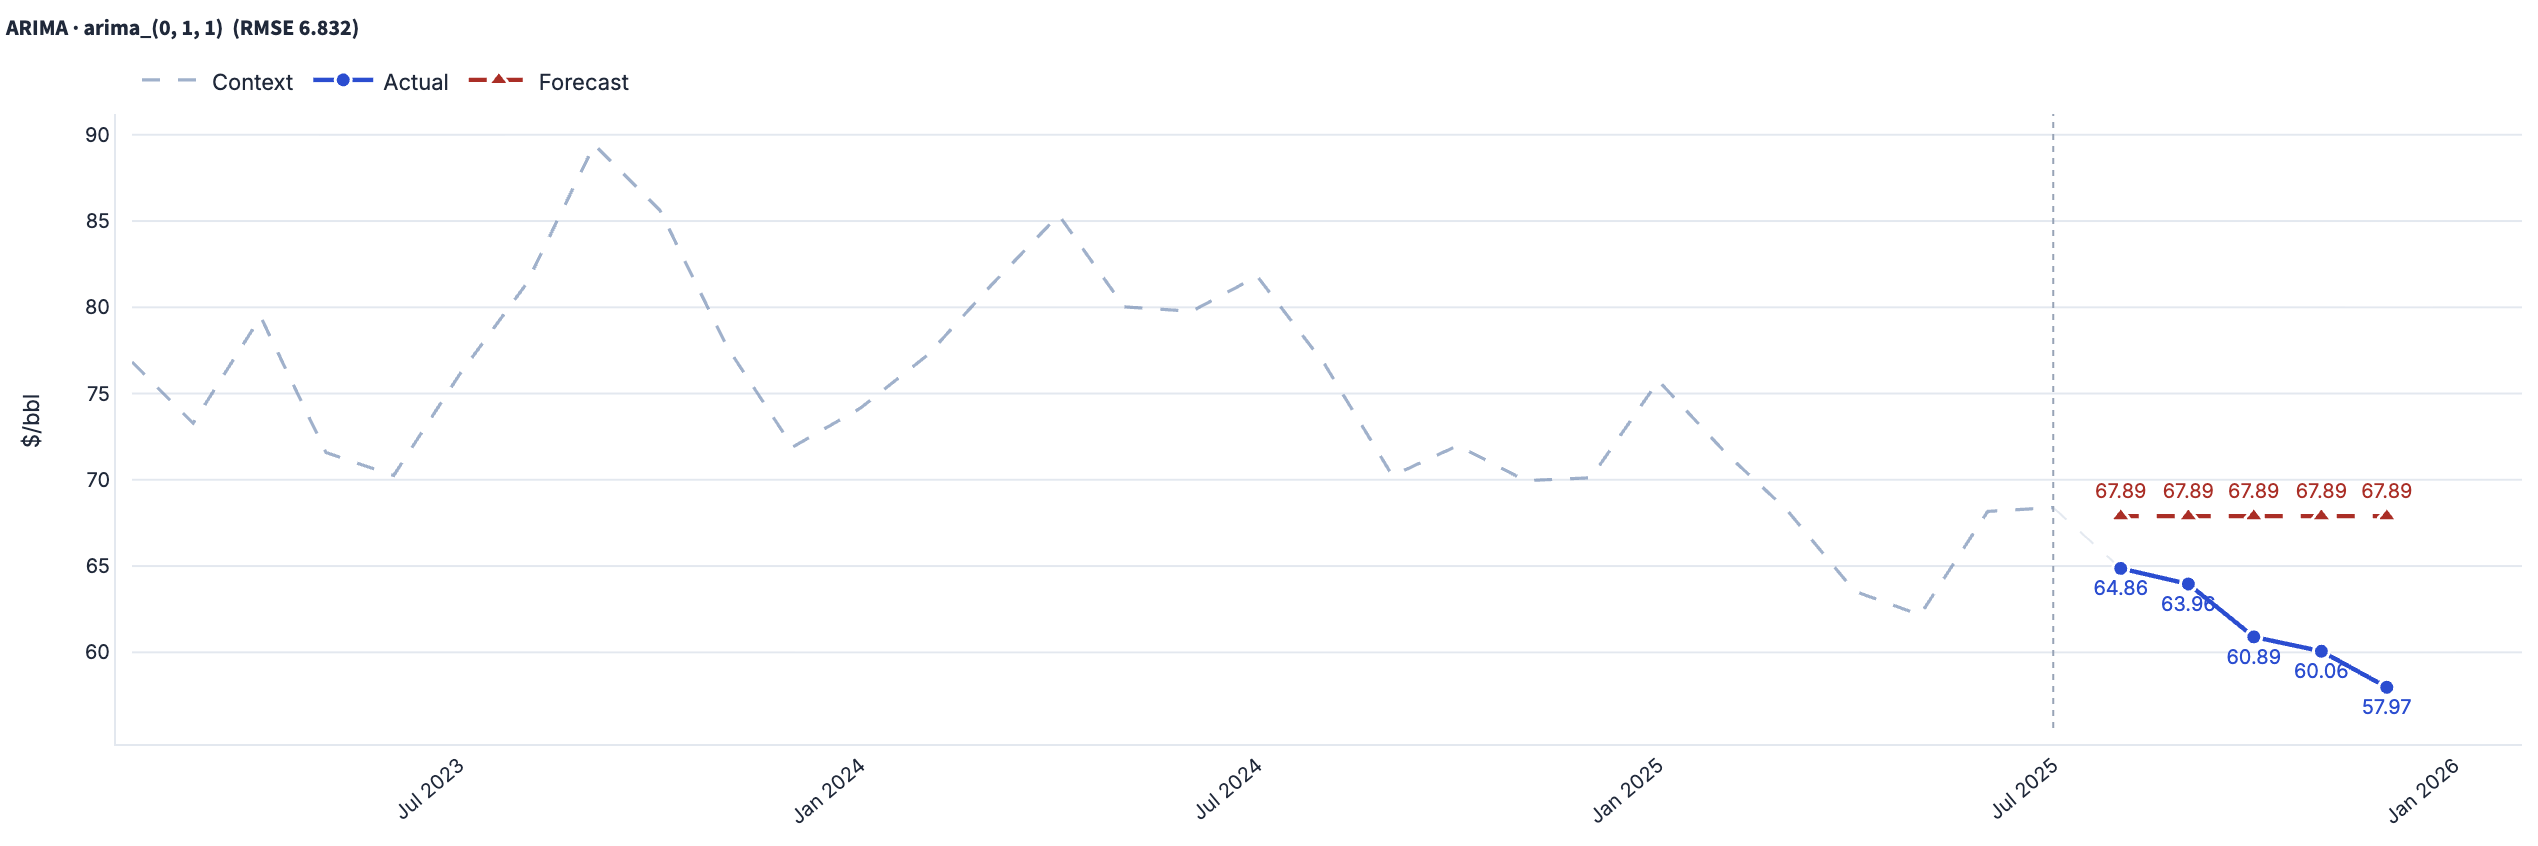
\includegraphics[width=\textwidth]{figures/univariate_arima_oil.png}
\small (a) ARIMA forecast for crude oil
\end{minipage}\hfill
\begin{minipage}[t]{0.48\textwidth}
\centering
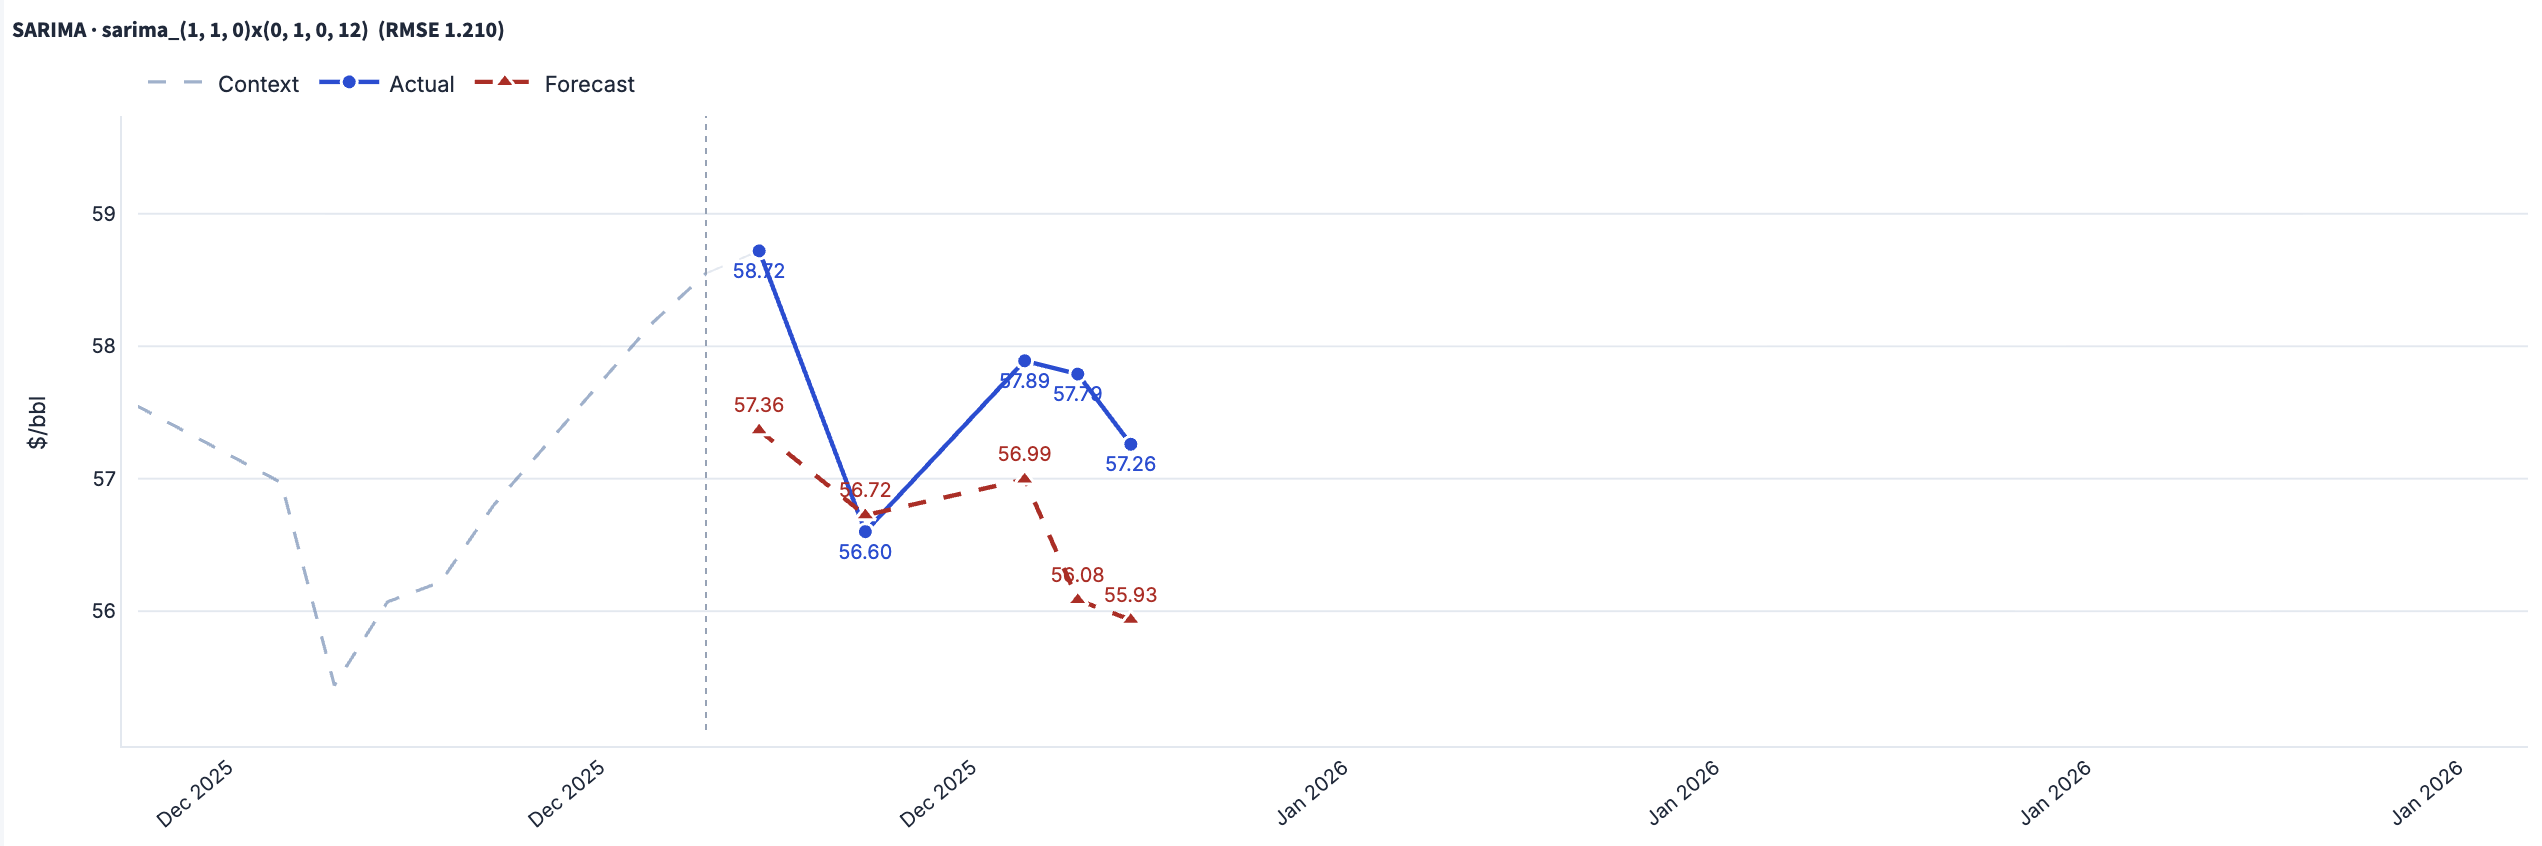
\includegraphics[width=\textwidth]{figures/univariate_sarima_oil.png}
\small (b) SARIMA forecast for crude oil
\end{minipage}

\vspace{0.5em}

\begin{minipage}[t]{0.48\textwidth}
\centering
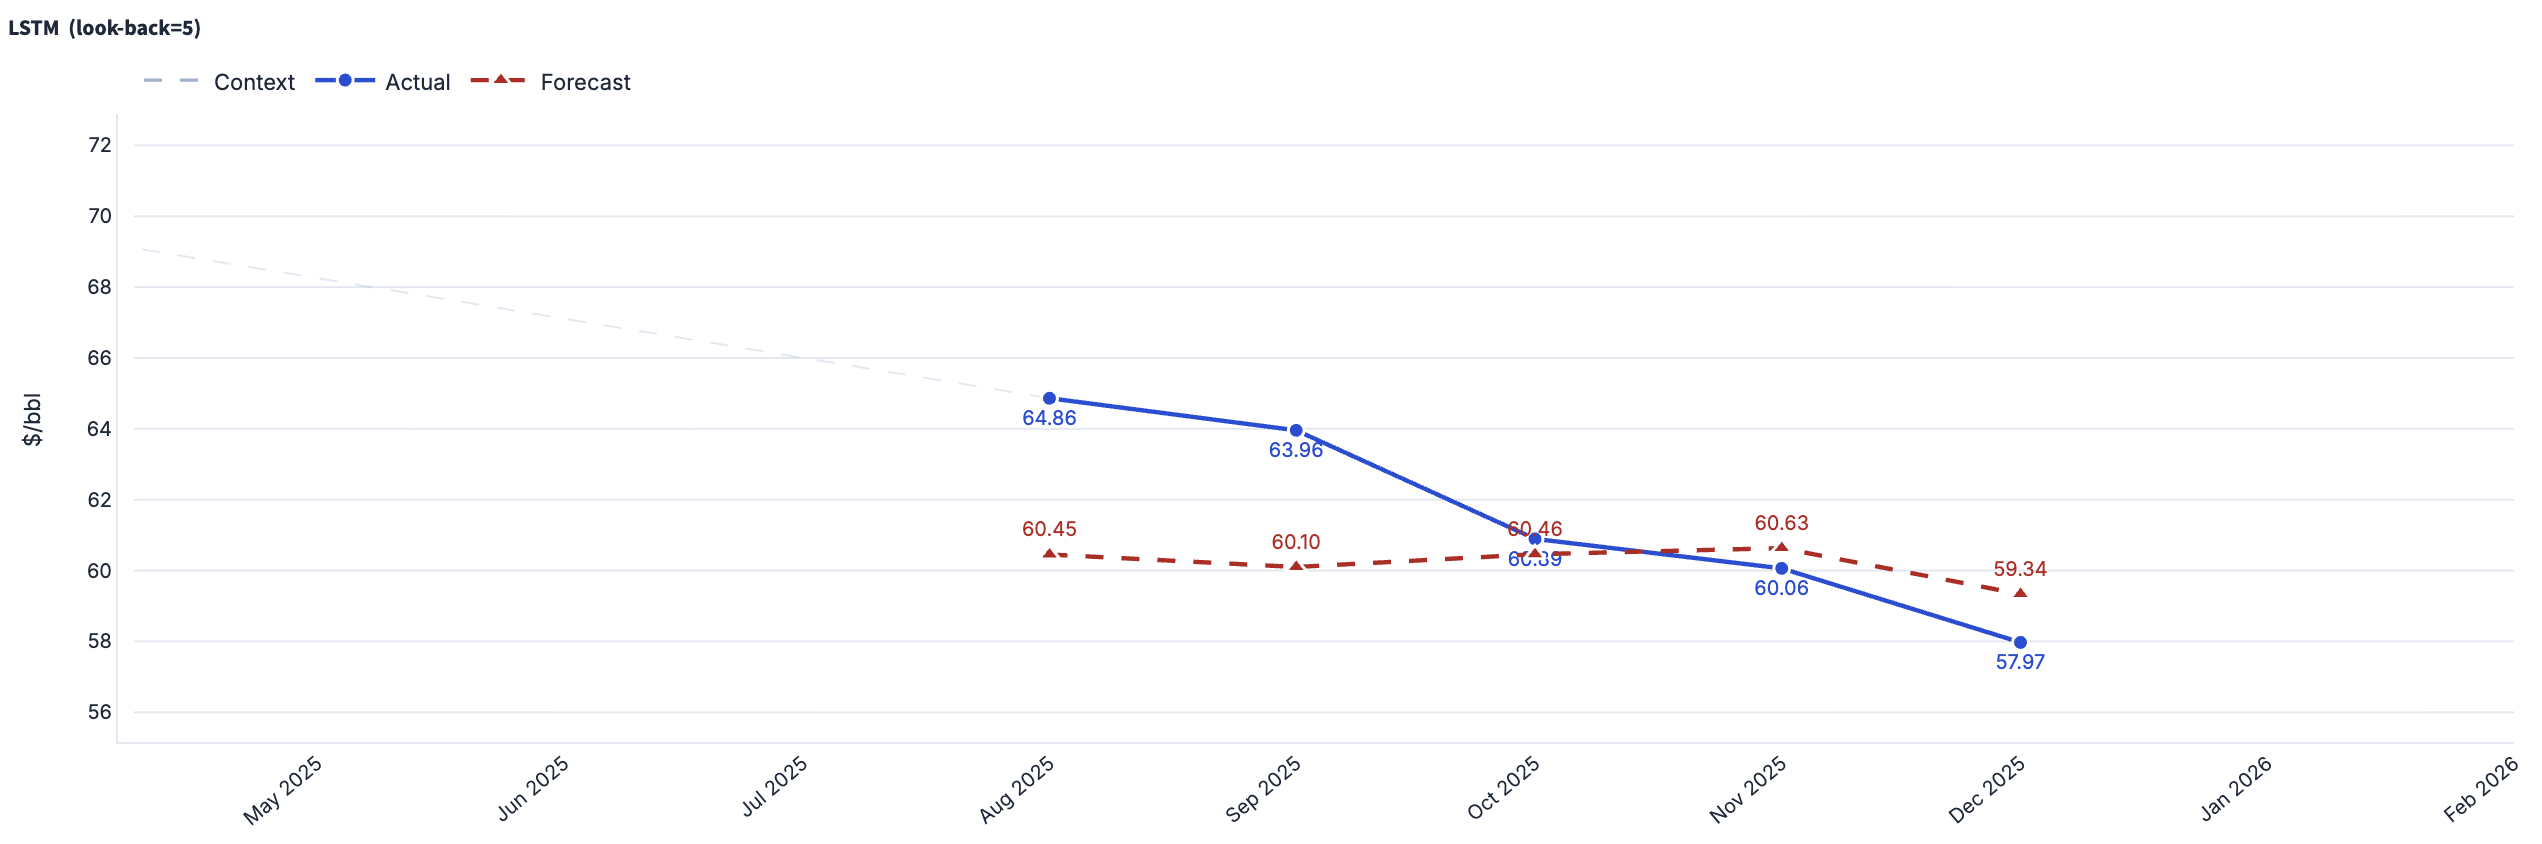
\includegraphics[width=\textwidth]{figures/univariate_oil_lstm_backtest.png}
\small (c) LSTM forecast for crude oil
\end{minipage}\hfill
\begin{minipage}[t]{0.48\textwidth}
\centering
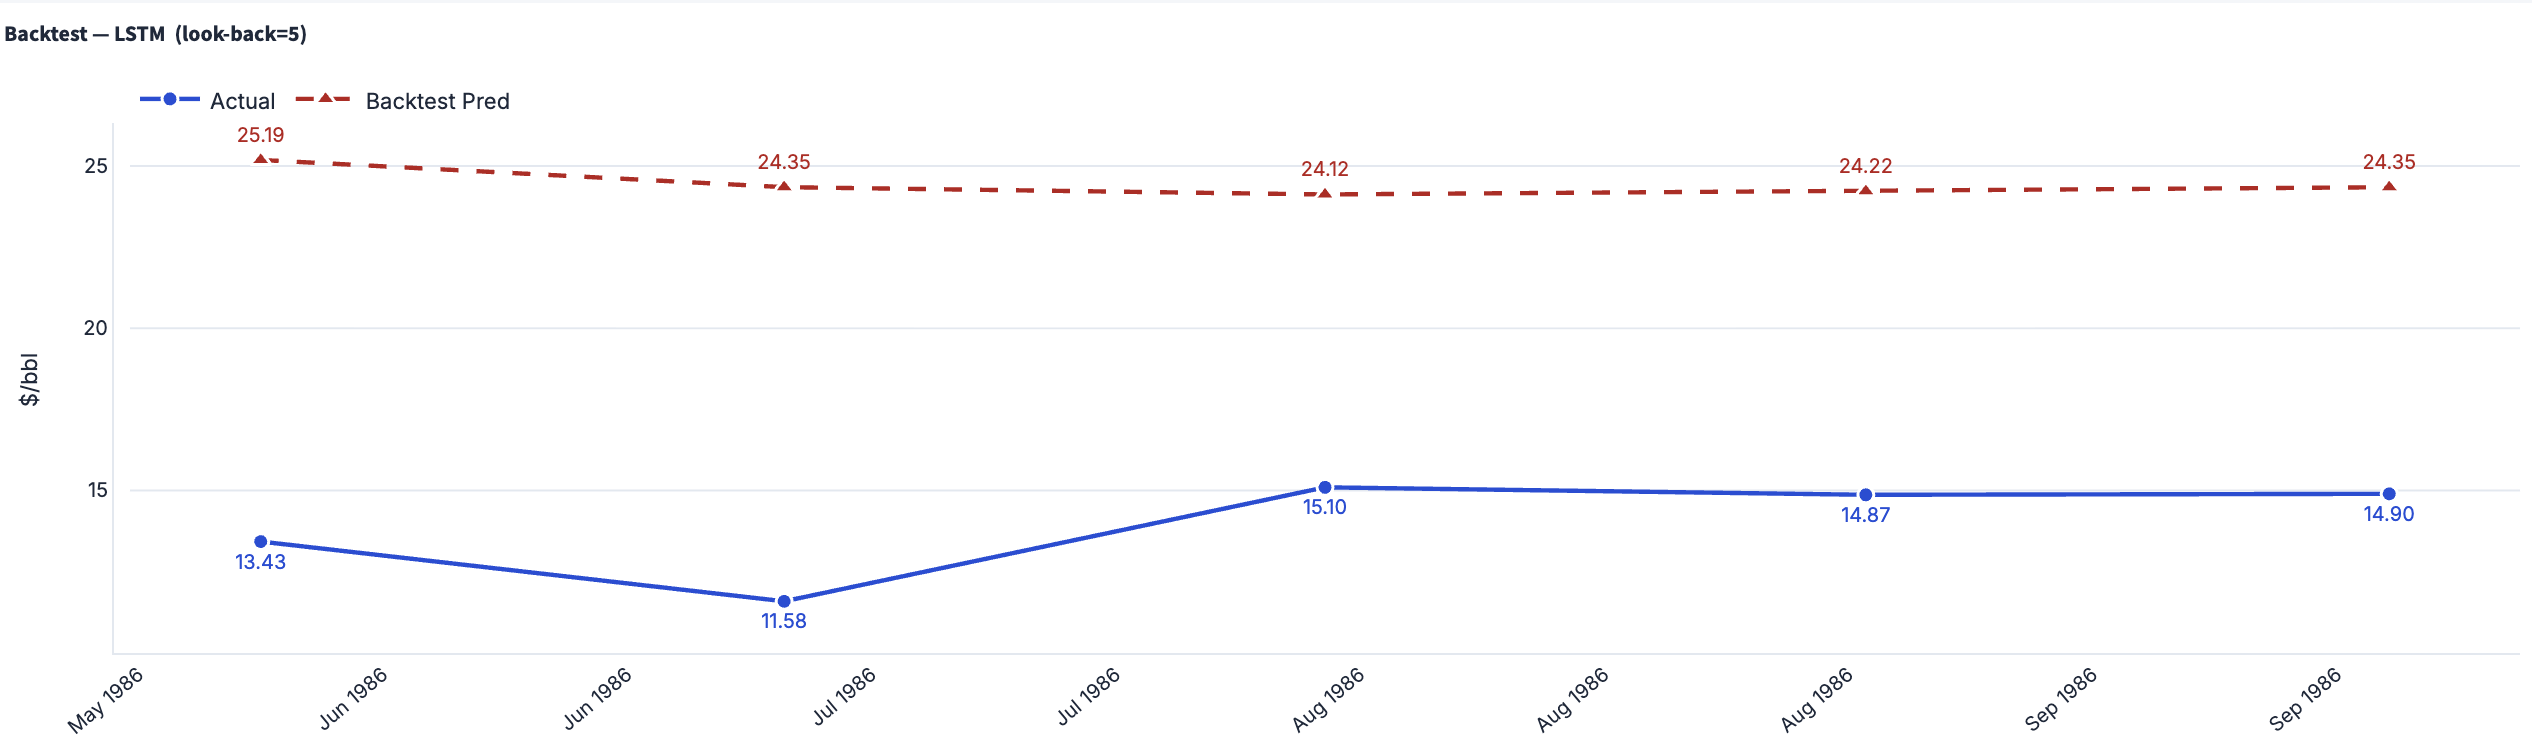
\includegraphics[width=\textwidth]{figures/univariate_oil_lstm.png}
\small (d) LSTM backtest for crude oil
\end{minipage}
\caption{Actual versus predicted WTI crude oil prices (USD/barrel, monthly, 2014--2024) across univariate model configurations: (a) ARIMA $(0,1,1)$, (b) SARIMA $(1,1,0) \times (0,1,0,12)$, (c) LSTM direct forecast, and (d) LSTM walk-forward backtest.}
\label{fig:univariate_crude_plots}
\end{figure}

\begin{table}[h]
\centering
\caption{Univariate model performance for crude oil}
\label{tab:univariate_crude}
\begin{tabular}{@{}lcccc@{}}
\toprule
Model & RMSE (USD/barrel) & MAE (USD/barrel) & MAPE (\%) & DA \\
\midrule
ARIMA & 6.832 & 6.343 & 10.49 & 0.20 \\
SARIMA & 1.210 & 1.081 & 1.87 & 0.60 \\
LSTM Forecast & 2.709 & 2.127 & -0.139 & 0.50 \\
LSTM Backtest & 10.578 & 10.471 & 76.78 & 0.10 \\
\botrule
\end{tabular}
\end{table}

As illustrated in Figure~\ref{fig:univariate_crude_plots}, the SARIMA model demonstrates the closest alignment with observed crude oil price dynamics, effectively tracking
seasonal cyclicality that the non-seasonal ARIMA specification and the LSTM model are unable to reproduce with comparable fidelity. In contrast, ARIMA produces smoother forecasts with limited responsiveness to fluctuations, while LSTM shows reasonable short-term tracking in the direct forecast setting but lacks consistency over time. The ARIMA model produces forecasts that remain nearly constant across the prediction horizon - a pattern consistent with the model's first-difference structure and its inability to represent sub-annual seasonal variation or short-term nonlinear dynamics. The SARIMA model improves this by incorporating seasonal structure, leading to forecasts that better follow the observed trend.

The LSTM forecasting plot shows smoother predictions that approximate the general level of the series but fail to respond to sharp changes. This suggests that the model does not adequately reproduce local variations. In the backtesting results, the LSTM predictions appear almost flat across rolling windows, while the actual series exhibits noticeable variability. This behavior leads to significantly higher RMSE and MAE values. The DA results reinforce this ranking: SARIMA reaches 0.60, outperforming ARIMA (0.20), LSTM forecast (0.50), and especially the LSTM backtest (0.10). Therefore, although backtesting is intended to verify temporal consistency, in this case it reveals that the model fails to represent non-trivial temporal dynamics and cannot be considered reliable for inference in the univariate setting. Overall, SARIMA performs better among the crude-oil univariate models in both error and directional terms.

\subsubsection*{5.1.2 Natural Gas (CNG)}\label{subsubsec:cngresults}

Table~\ref{tab:univariate_gas} and Figure~\ref{fig:univariate_gas_plots} summarize the natural-gas results by comparing the actual and predicted prices across ARIMA, SARIMA, and LSTM-based models.

\begin{figure}[h]
\centering
\begin{minipage}[t]{0.48\textwidth}
\centering
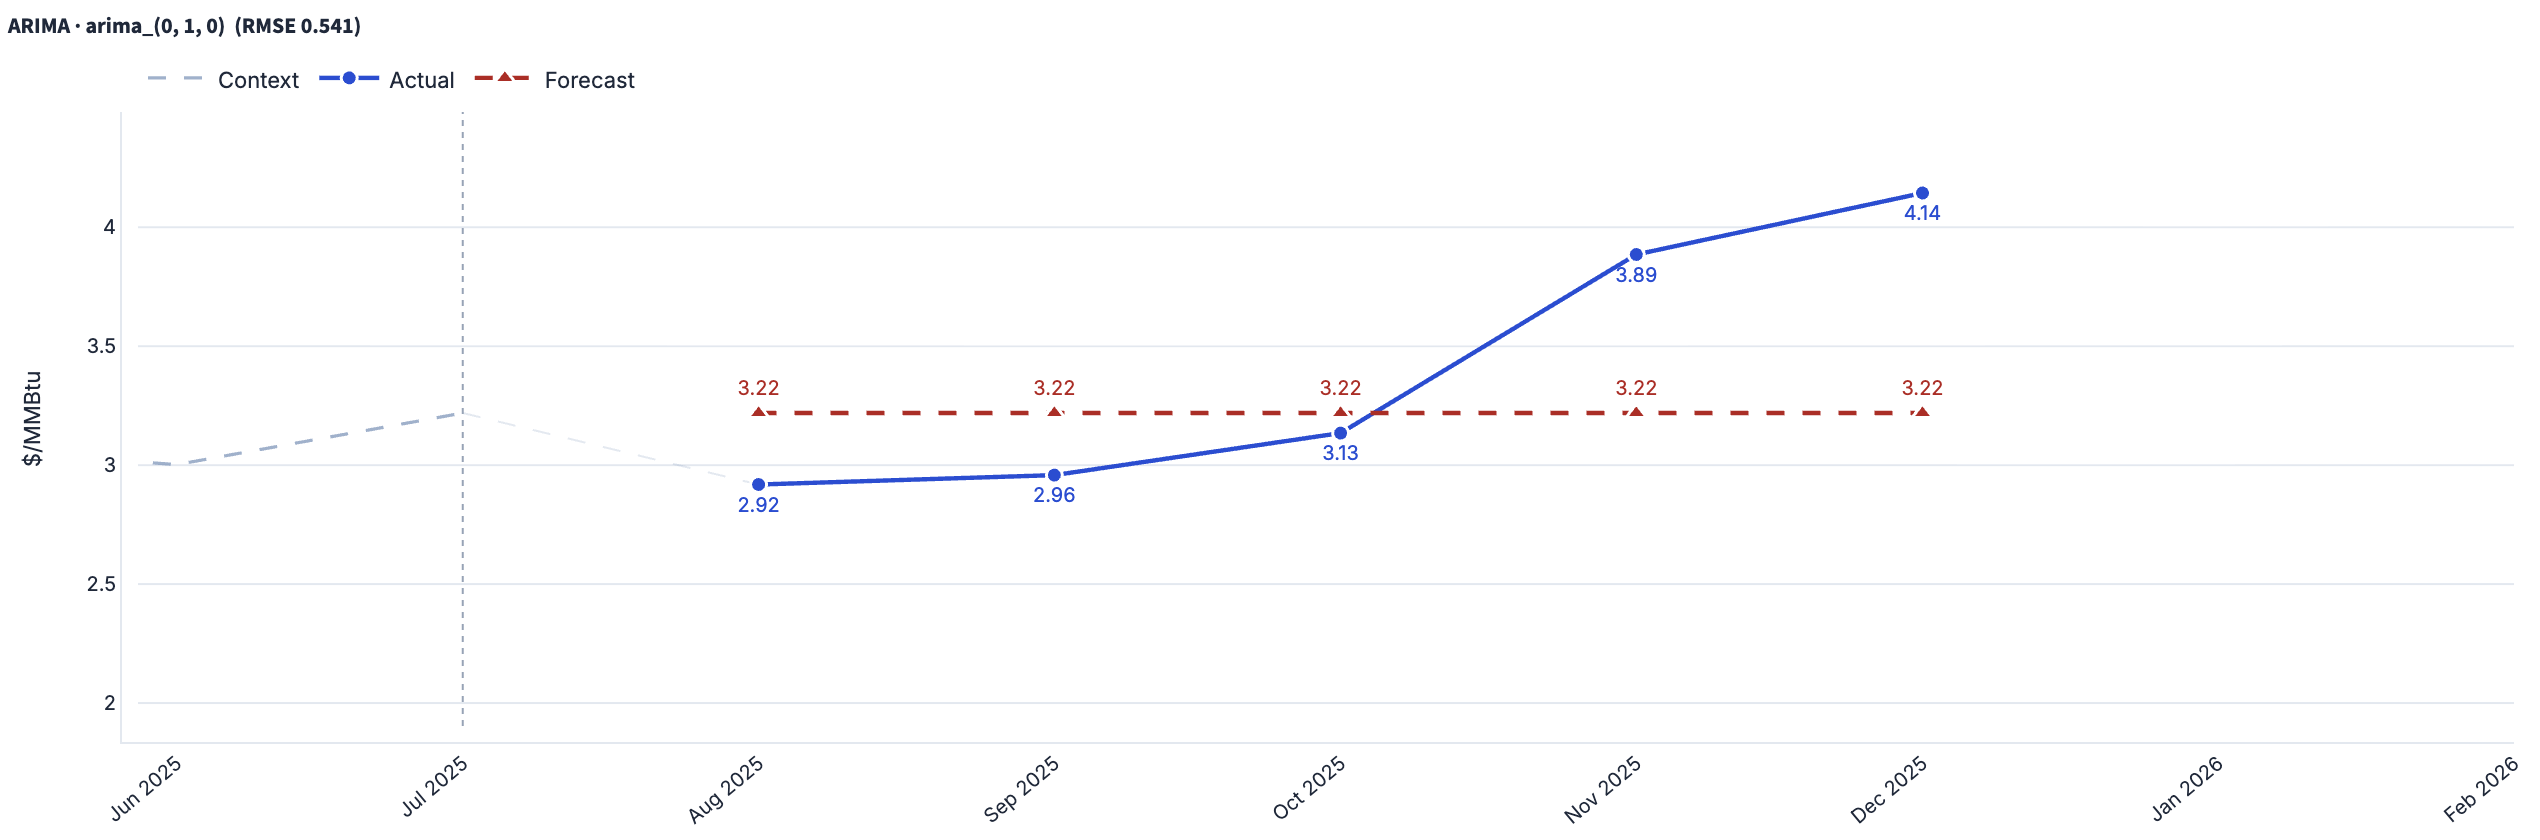
\includegraphics[width=\textwidth]{figures/univariate_arima_cng.png}
\small (a) ARIMA forecast for natural gas
\end{minipage}\hfill
\begin{minipage}[t]{0.48\textwidth}
\centering
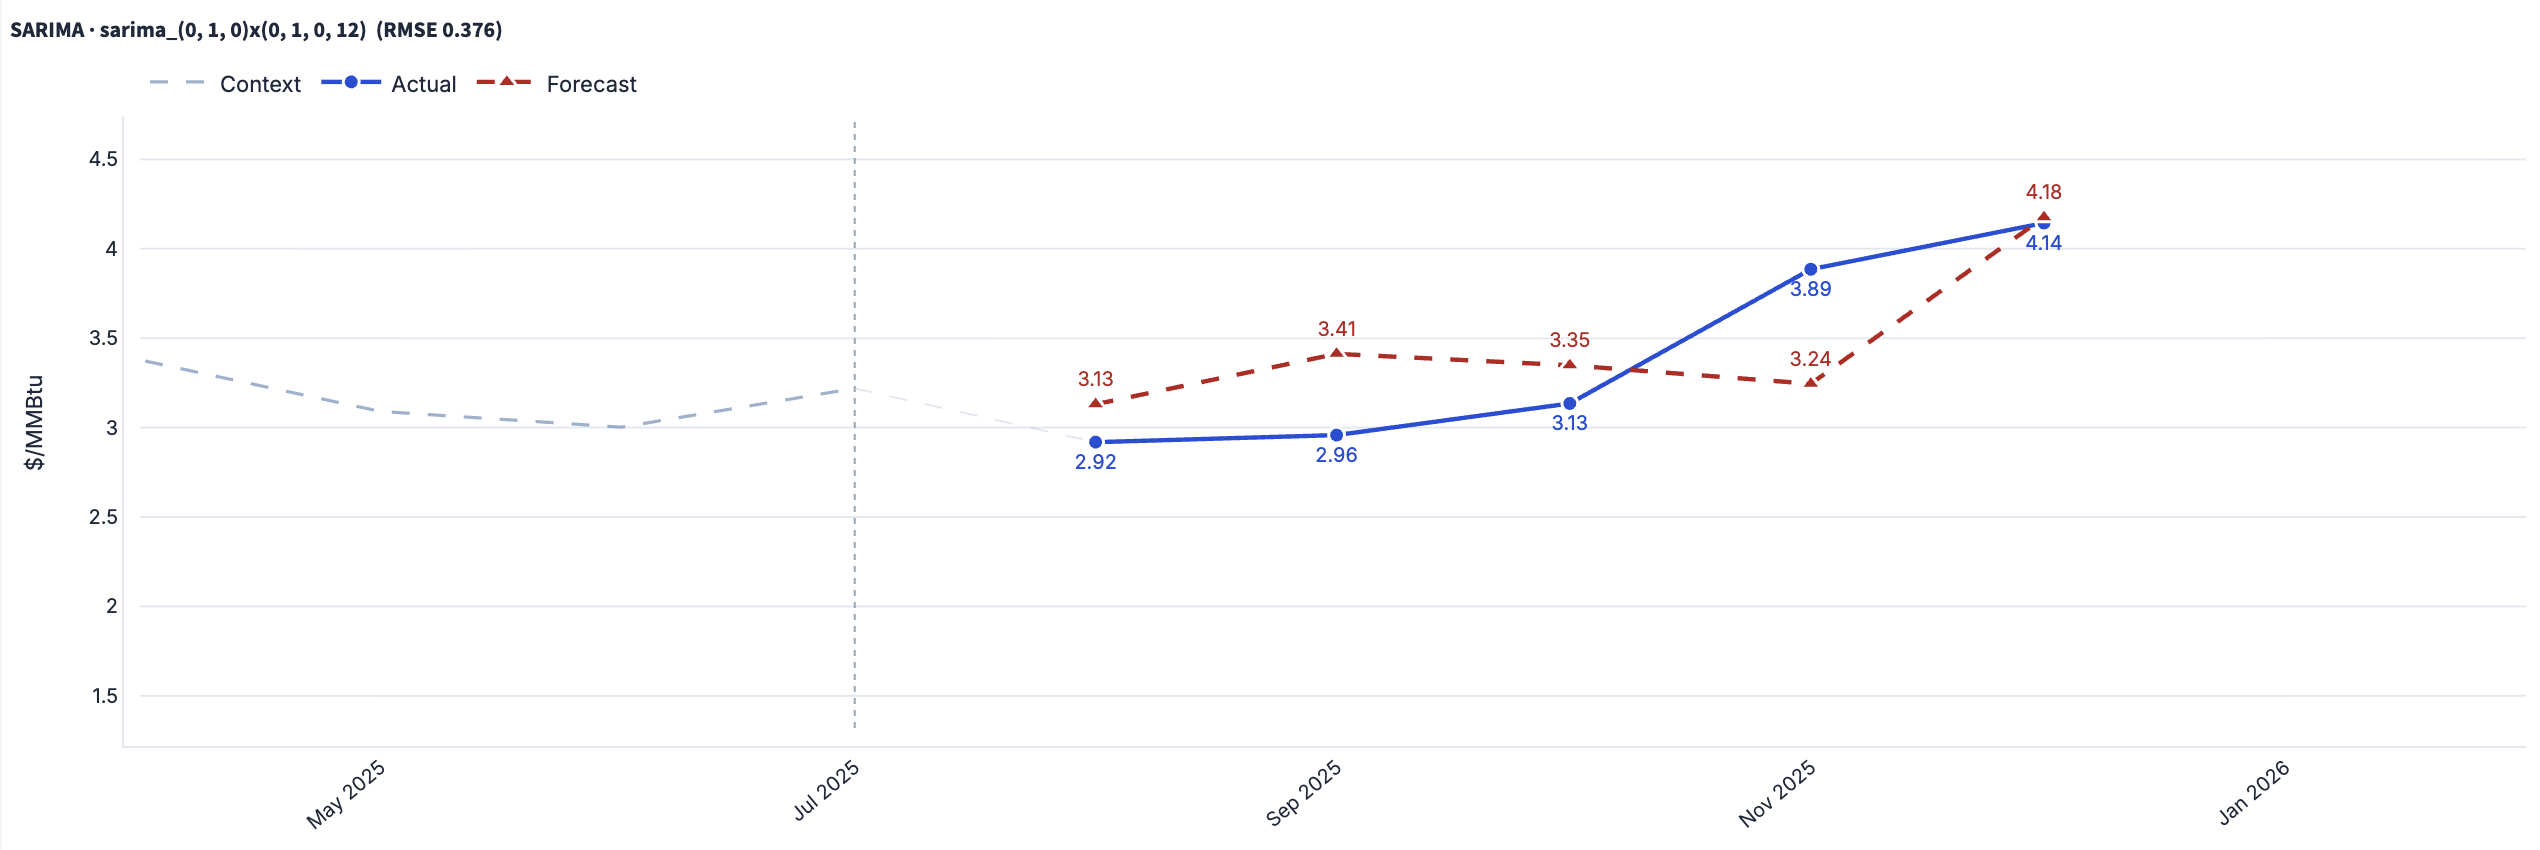
\includegraphics[width=\textwidth]{figures/univariate_sarima_cng.png}
\small (b) SARIMA forecast for natural gas
\end{minipage}

\vspace{0.5em}

\begin{minipage}[t]{0.48\textwidth}
\centering
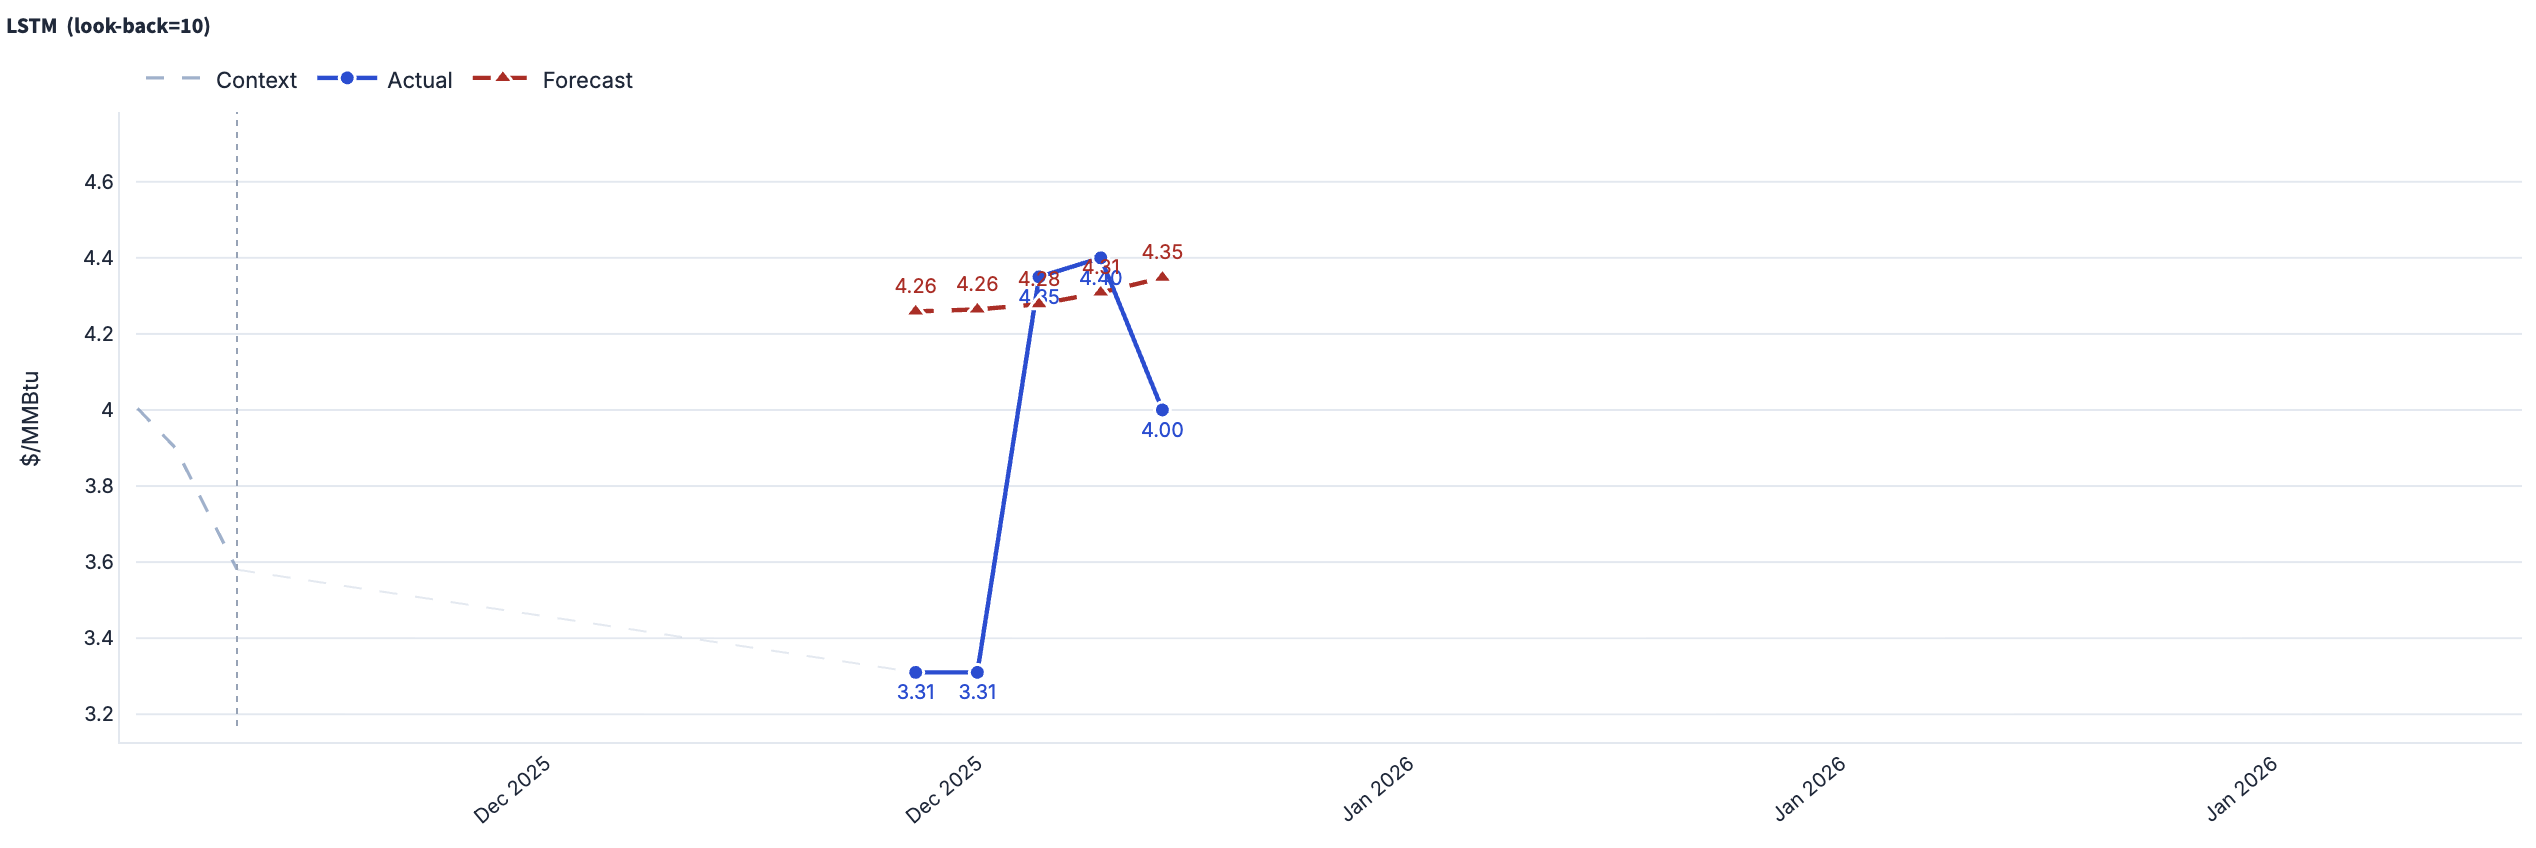
\includegraphics[width=\textwidth]{figures/univariate_cng_lstm.png}
\small (c) LSTM forecast for natural gas
\end{minipage}\hfill
\begin{minipage}[t]{0.48\textwidth}
\centering
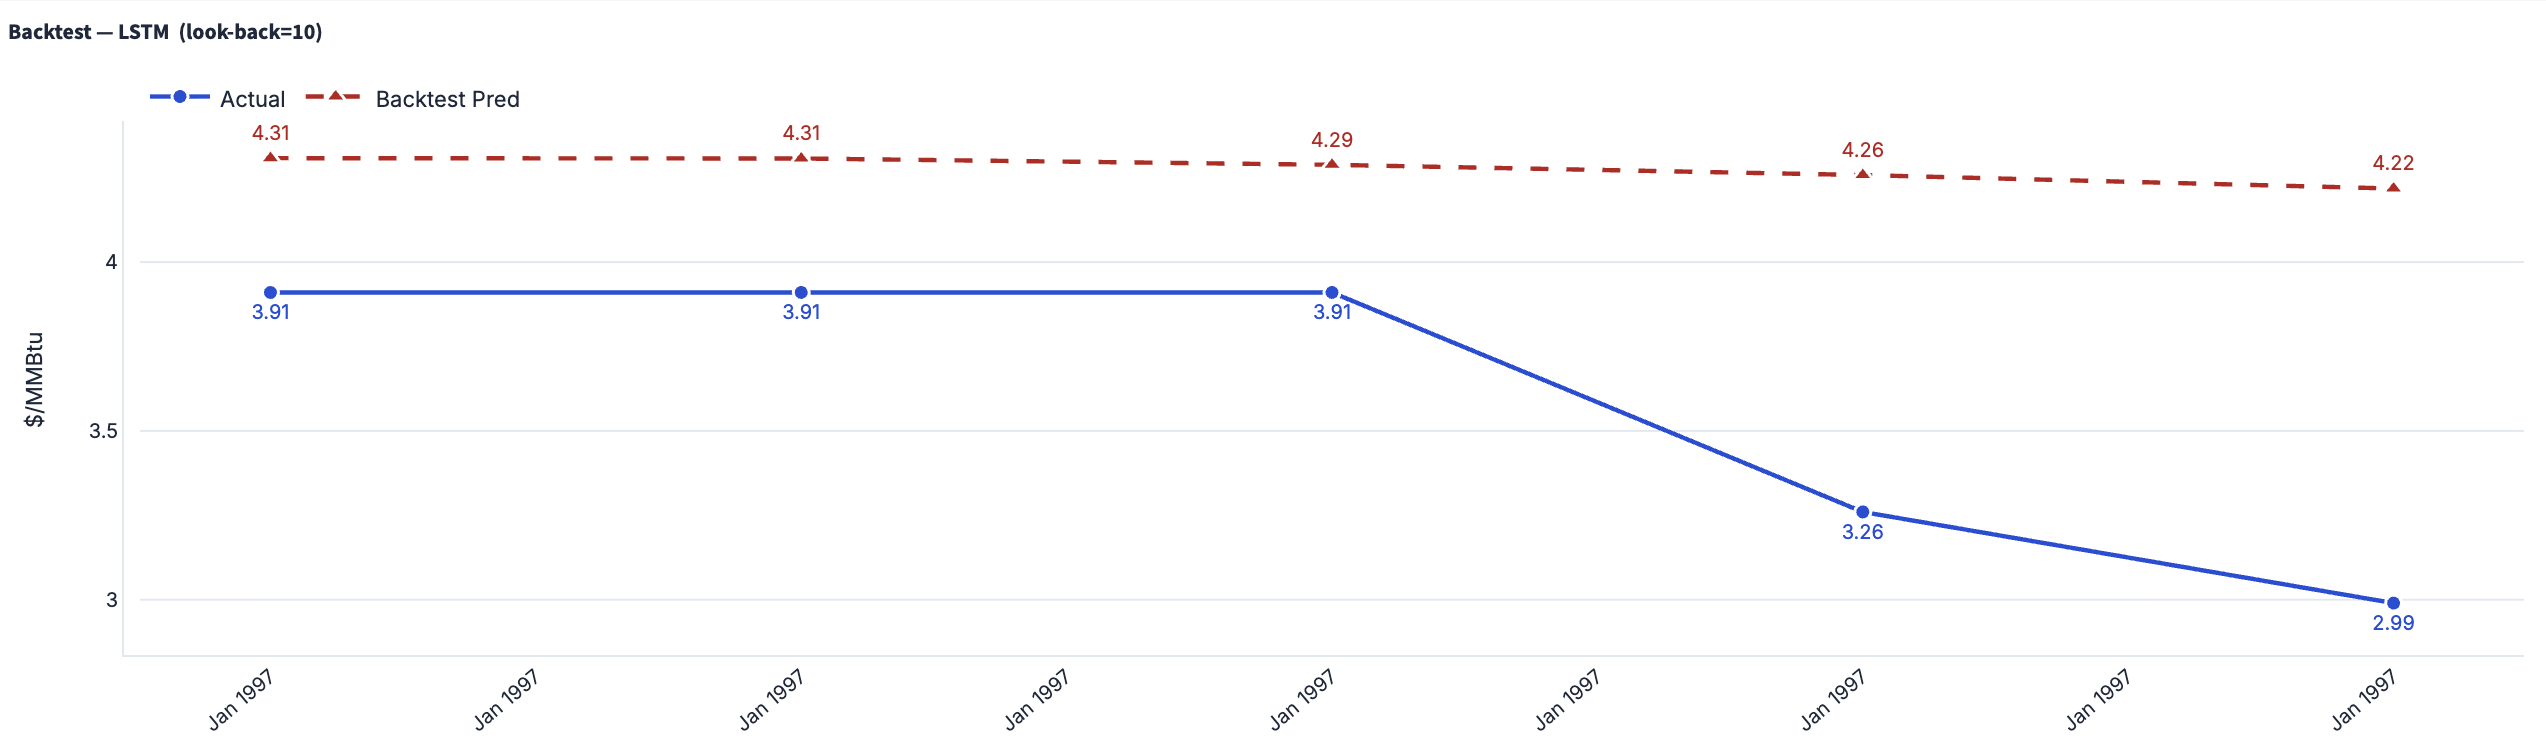
\includegraphics[width=\textwidth]{figures/univariate_cng_lstm_backtest.png}
\small (d) LSTM backtest for natural gas
\end{minipage}
\caption{Actual versus predicted Henry Hub natural gas prices (USD/MMBtu, monthly, 2014--2024) across univariate model configurations: (a) ARIMA $(0,1,0)$, (b) SARIMA $(0,1,0) \times (0,1,0,12)$, (c) LSTM direct forecast, and (d) LSTM walk-forward backtest.}
\label{fig:univariate_gas_plots}
\end{figure}

\begin{table}[h]
\centering
\caption{Univariate model performance for natural gas}
\label{tab:univariate_gas}
\begin{tabular}{@{}lcccc@{}}
\toprule
Model & RMSE (USD/MMBtu) & MAE (USD/MMBtu) & MAPE (\%) & DA \\
\midrule
ARIMA & 0.541 & 0.447 & 12.26 & 0.40 \\
SARIMA & 0.376 & 0.310 & 9.34 & 0.80 \\
LSTM Forecast & 0.624 & 0.483 & 13.99 & 0.60 \\
LSTM Backtest & 0.770 & 0.680 & 20.33 & 0.00 \\
\botrule
\end{tabular}
\end{table}

As shown in Figure~\ref{fig:univariate_gas_plots}, SARIMA again demonstrates superior performance by effectively tracking seasonal patterns in natural gas prices. ARIMA underfits the data, while LSTM exhibits moderate forecasting ability but reduced stability across time.

For natural gas (CNG), ARIMA again produces flat forecasts, while SARIMA better tracks the overall trend and seasonal movement. The LSTM forecasting results show noticeable deviation from actual values, indicating difficulty in modeling the series. In the  backtesting plots, predictions are relatively flat compared to the actual fluctuations, resulting in higher error. The DA values again favor SARIMA, which attains 0.80 versus 0.40 for ARIMA, 0.60 for the LSTM forecast, and 0.00 for the LSTM backtest. This suggests that the LSTM model does not generalize well across time and struggles to reproduce variability in the absence of additional explanatory features.

Overall, while SARIMA exhibits comparatively superior performance among the univariate model class, none of the approaches evaluated consistently reproduce the full range of variability and dynamic behavior exhibited by either energy price series - a finding that motivates the multivariate feature configurations examined in subsequent sections. These findings indicate that relying solely on historical price data is insufficient for robust forecasting, highlighting the need for incorporating additional explanatory variables to improve model performance.

\subsection{Multivariate Modelling}\label{subsec:multivariate_models}

This subsection presents the multivariate forecasting models developed by incorporating exogenous variables in addition to historical price data. The purpose of these models is to evaluate whether macroeconomic indicators, news-derived signals, or their combination improve forecasting performance beyond the univariate baselines. The models considered include SARIMAX, LSTM, and a hybrid CNN--LSTM architecture. To ensure robustness and reduce redundancy, multicollinearity among macroeconomic variables was assessed using the Variance Inflation Factor (VIF), as defined in Section~\ref{subsubsec:fredprocessing}, and variables with VIF greater than 8 were removed.

\subsubsection*{5.2.1 Macro Only}

In this setting, only macroeconomic variables were used as input features, excluding the target price series. To improve stability and reduce redundancy, multicollinearity among the macroeconomic variables was evaluated using the Variance Inflation Factor (VIF), and variables with VIF greater than 8 were removed before model fitting. The models evaluated in this setting were SARIMAX, LSTM, and CNN--LSTM. For the neural models, both LSTM and CNN--LSTM were trained using an input window of 36 time steps and a single-step output.

\subsubsection*{5.2.1.1 Crude Oil}
For crude oil, we evaluated SARIMAX, LSTM, and CNN--LSTM models using macroeconomic features. Table~\ref{tab:macro_only_oil} summarizes the performance results, and Figure~\ref{fig:macro_only_oil_plots} shows the corresponding predictions.

\begin{figure}[h]
\centering
\begin{minipage}[t]{0.48\textwidth}
\centering
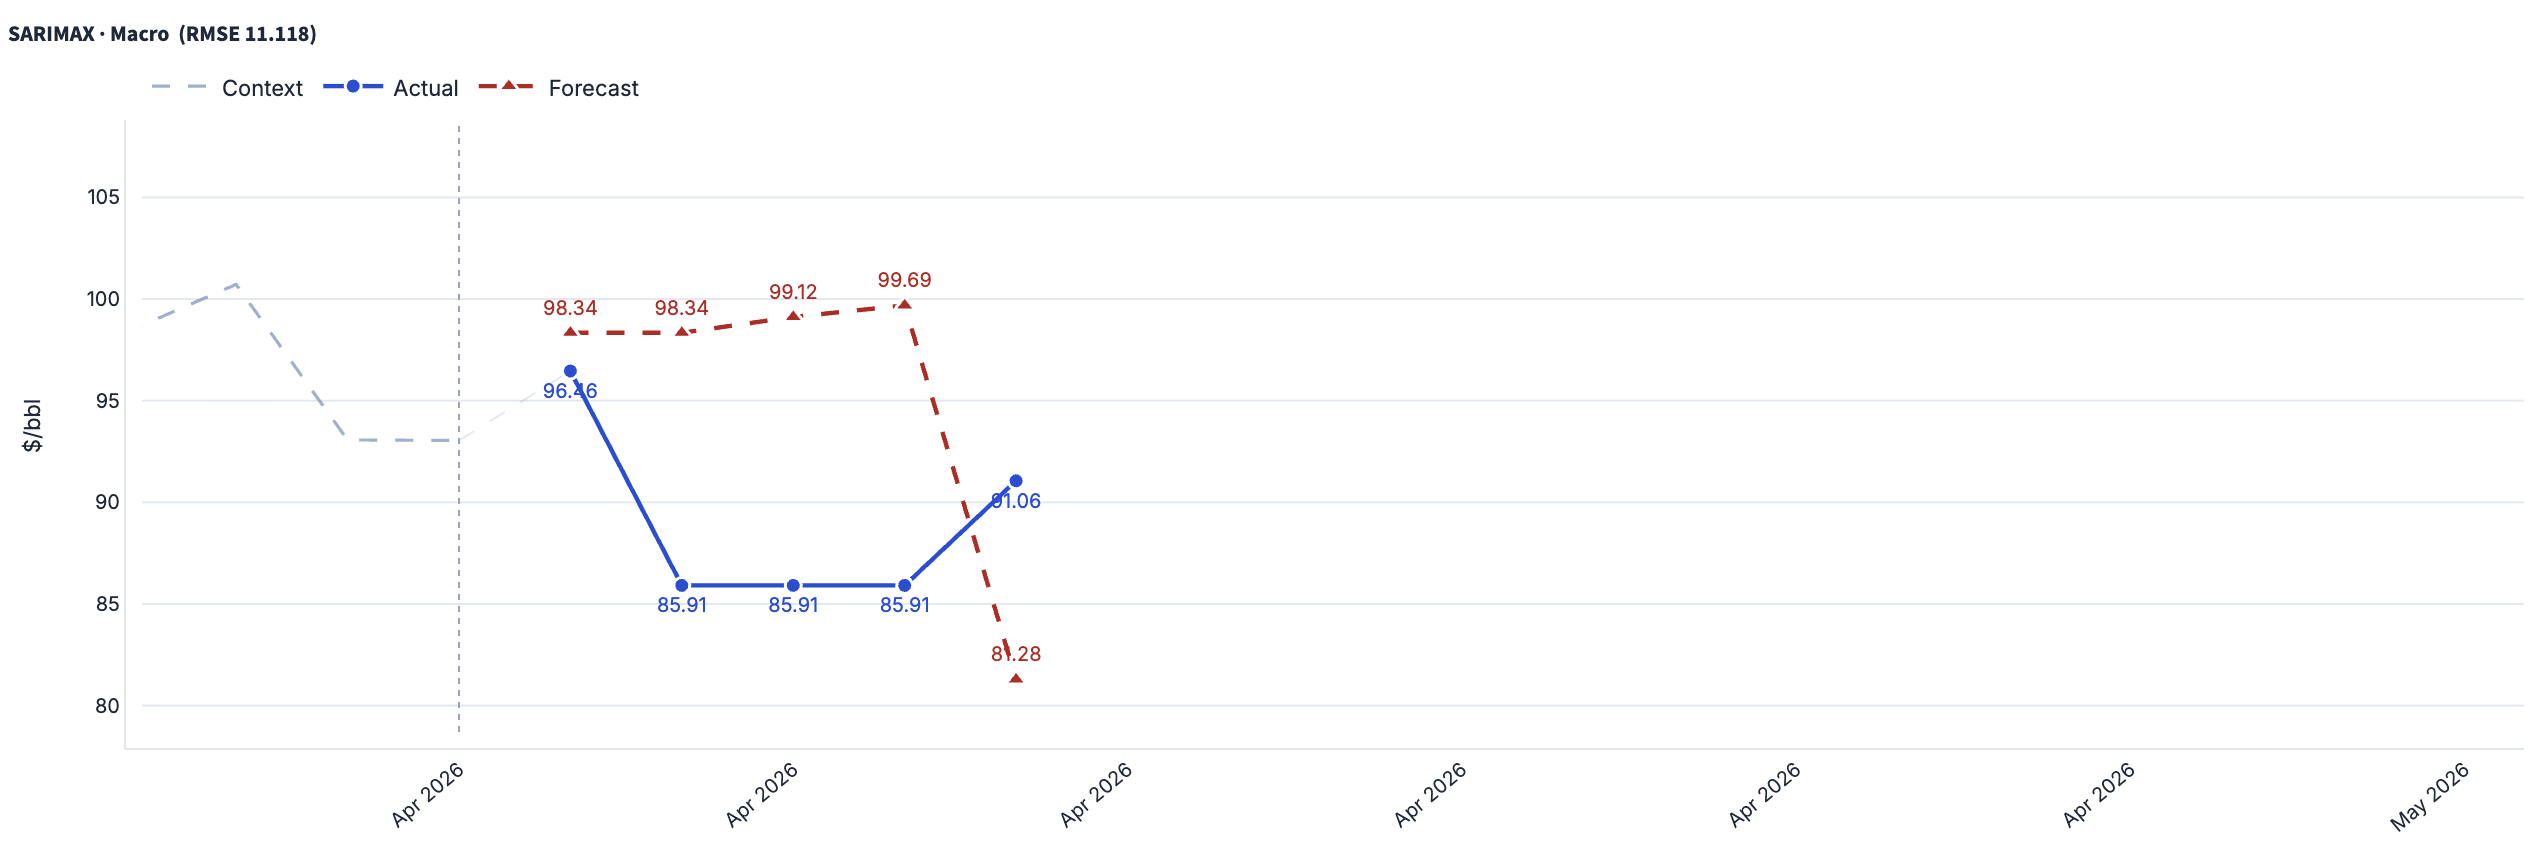
\includegraphics[width=\textwidth]{figures/multivariate_macro_oil_sarimax.png}
\small (a) SARIMAX forecast for crude oil
\end{minipage}\hfill
\begin{minipage}[t]{0.48\textwidth}
\centering
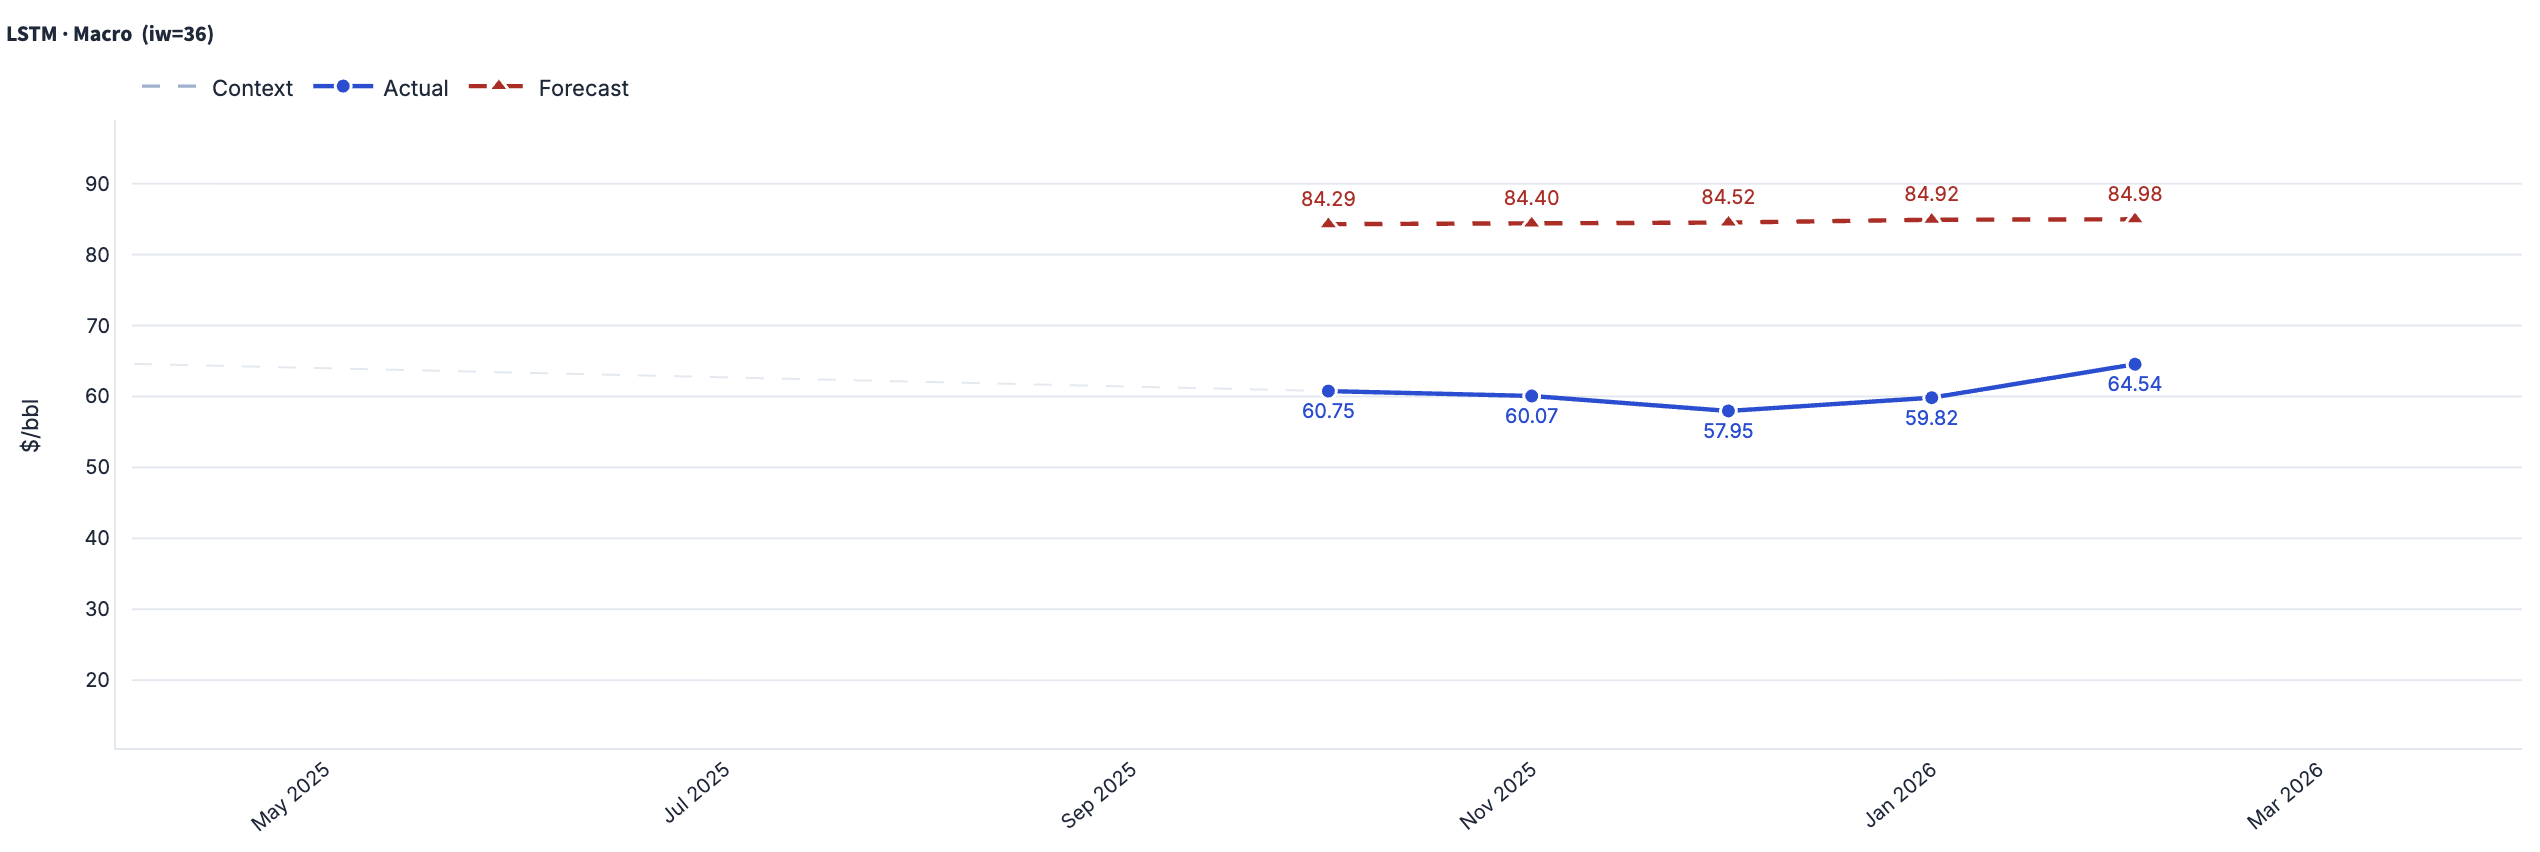
\includegraphics[width=\textwidth]{figures/multivaiate_macro_oil_lstm.png}
\small (b) LSTM forecast for crude oil
\end{minipage}

\vspace{0.5em}

\begin{minipage}[t]{0.48\textwidth}
\centering
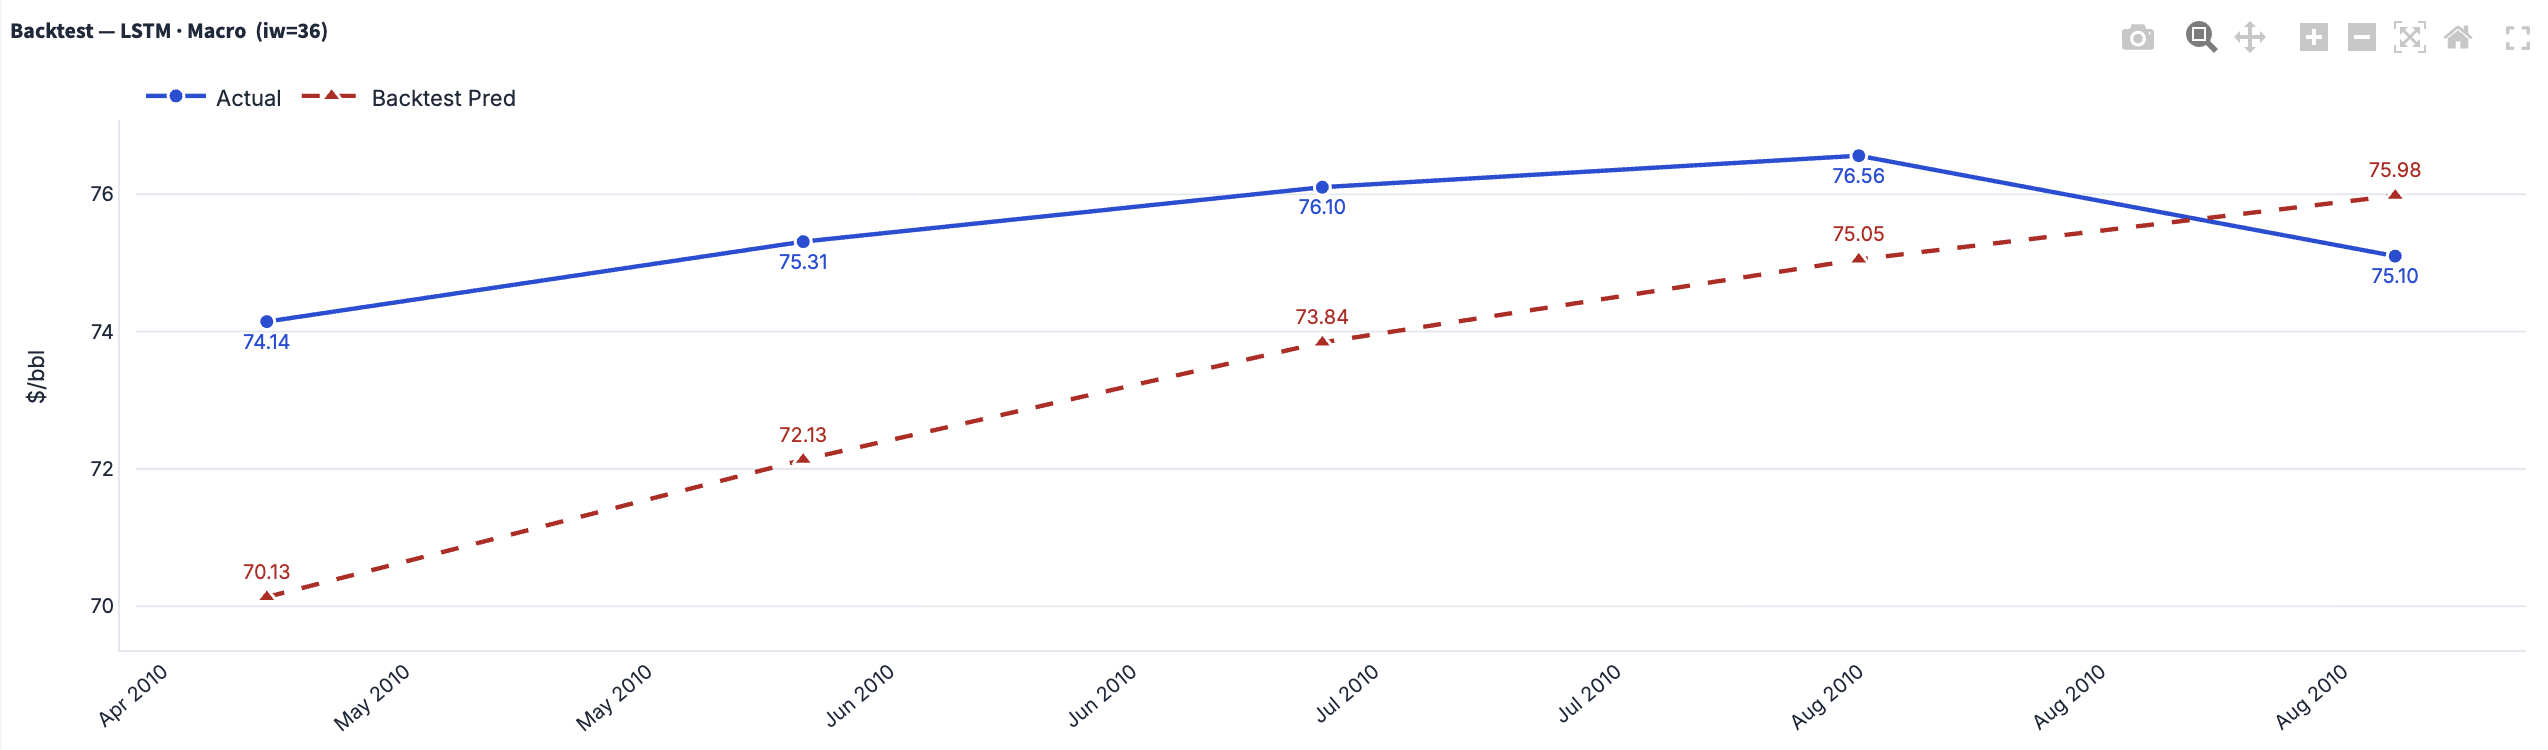
\includegraphics[width=\textwidth]{figures/multivariate_macro_oil_lstm_backtest.png}
\small (c) LSTM backtest for crude oil
\end{minipage}\hfill
\begin{minipage}[t]{0.48\textwidth}
\centering
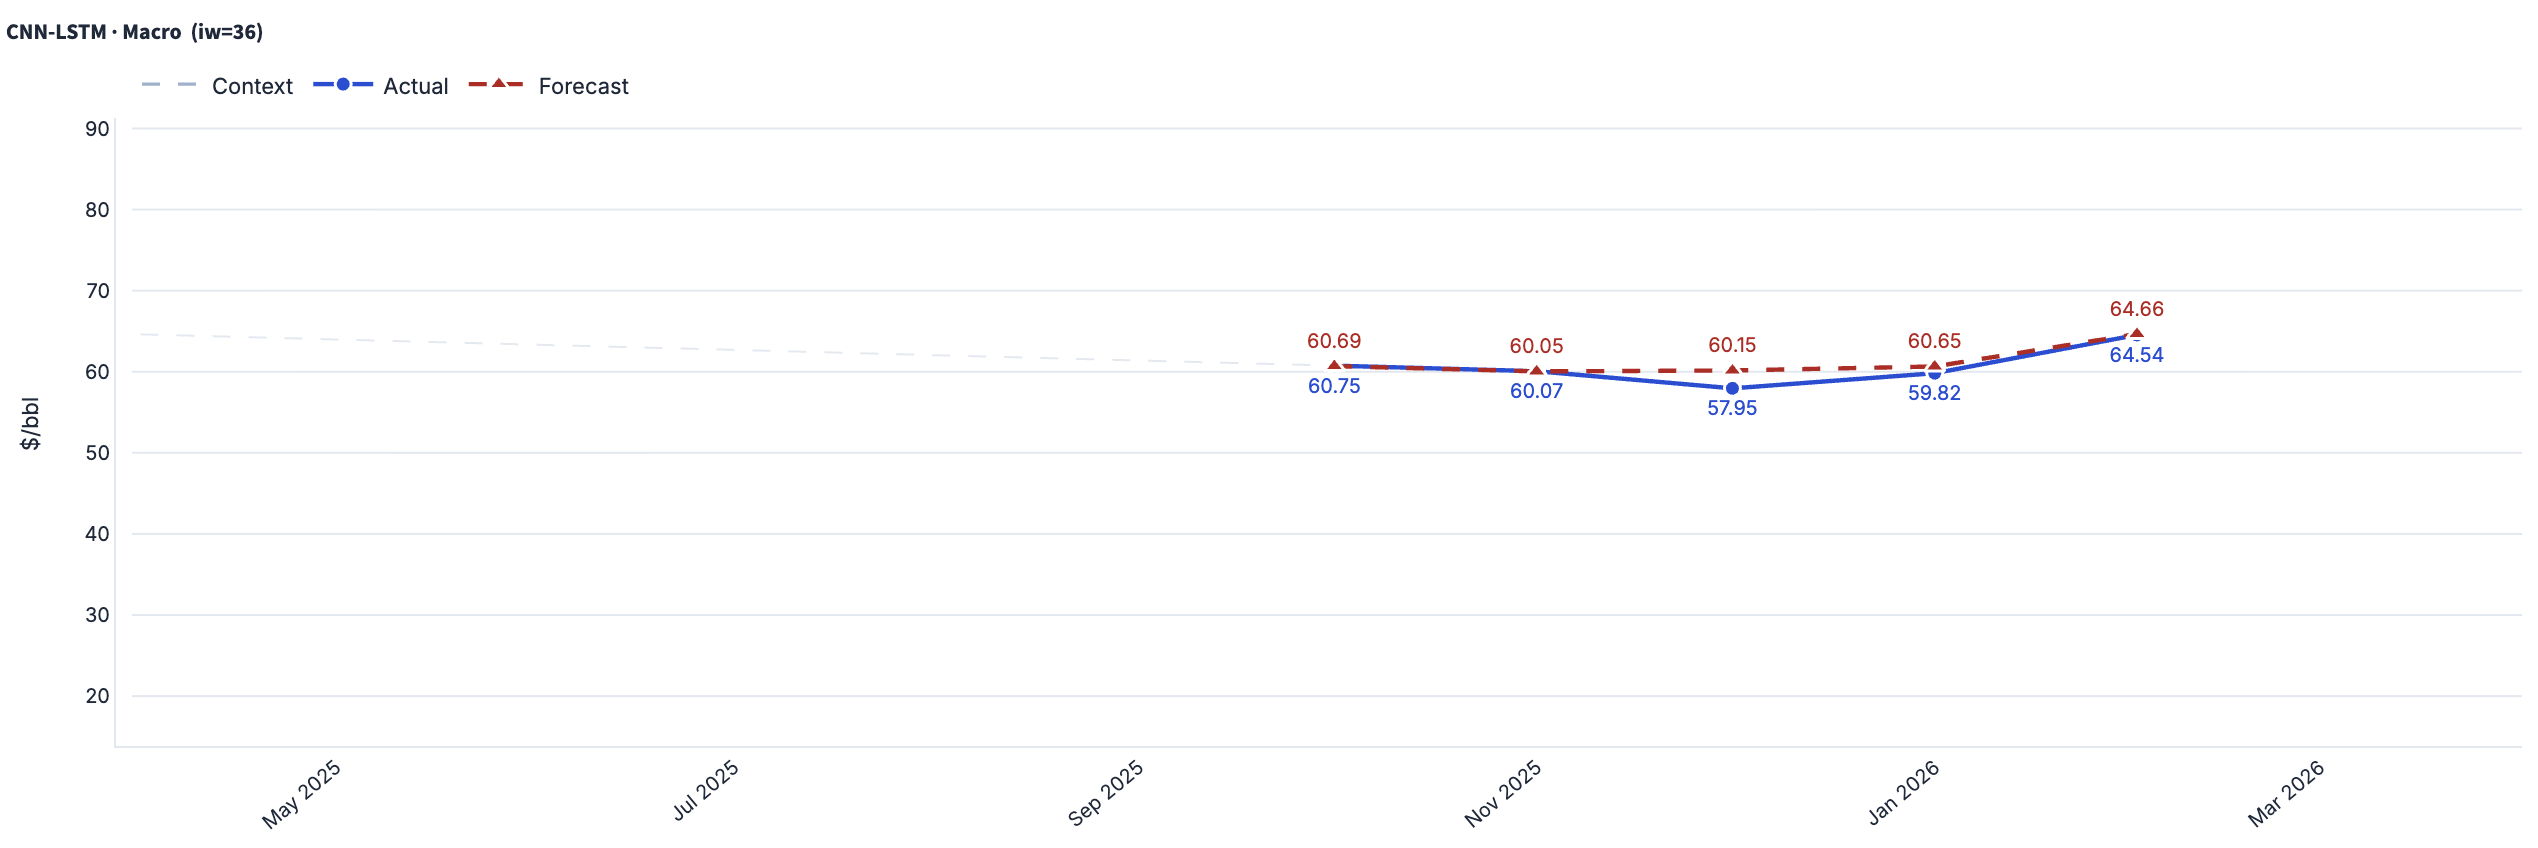
\includegraphics[width=\textwidth]{figures/multivariate_macro_oil_cnnlstm.png}
\small (d) CNN--LSTM forecast for crude oil
\end{minipage}

\vspace{0.5em}

\begin{minipage}[t]{0.48\textwidth}
\centering
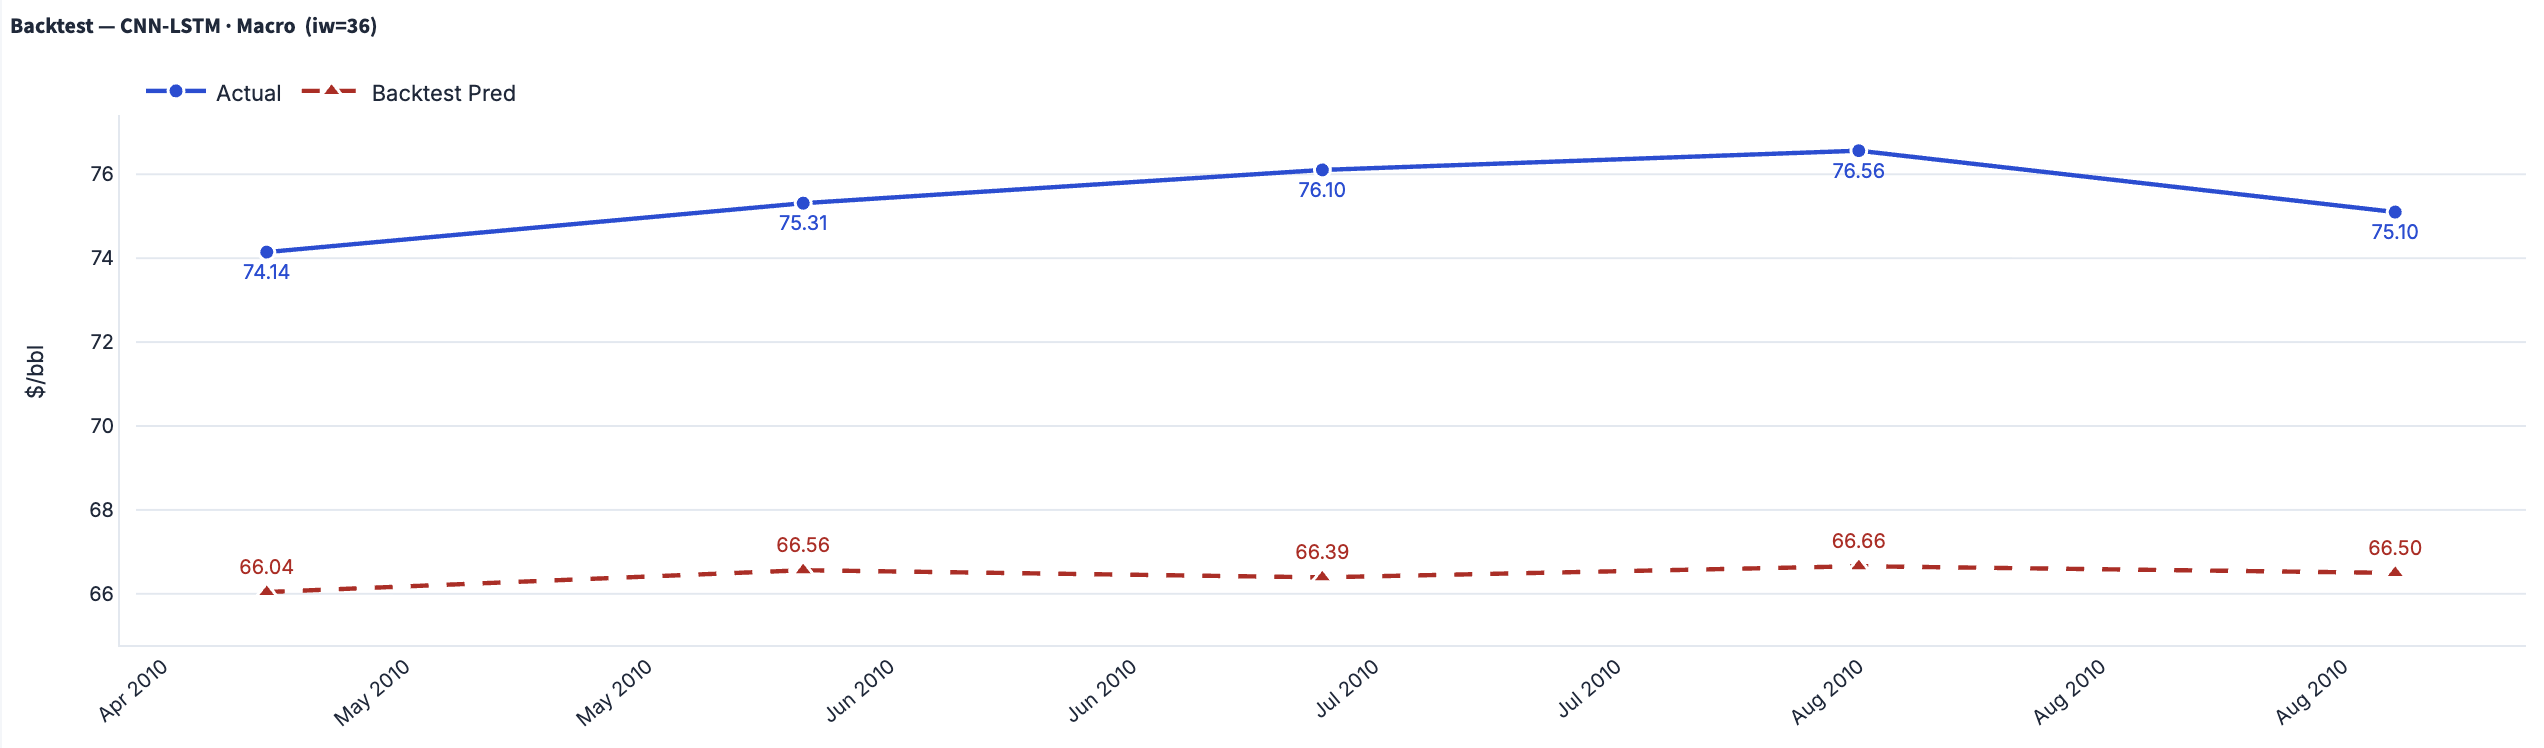
\includegraphics[width=\textwidth]{figures/multivariate_macro_oil_cnnlstm_backtest.png}
\small (e) CNN--LSTM backtest for crude oil
\end{minipage}
\caption{Actual versus predicted WTI crude oil prices (USD/barrel) using macroeconomic variables only: (a) SARIMAX forecast with exogenous FRED indicators, (b) LSTM direct forecast, (c) LSTM walk-forward backtest, (d) CNN--LSTM direct forecast, and (e) CNN--LSTM walk-forward backtest. This figure summarizes the macro-only multivariate setting.}
\label{fig:macro_only_oil_plots}
\end{figure}

\begin{table}[h]
\centering
\caption{Macro-only multivariate model performance for crude oil}
\label{tab:macro_only_oil}
\begin{tabular}{@{}lcccc@{}}
\toprule
Model & RMSE (USD/barrel) & MAE (USD/barrel) & MAPE (\%) & DA \\
\midrule
SARIMAX & 24.081 & 23.995 & 39.74 & 0.40 \\
LSTM Forecast & 24.081 & 23.995 & 39.74 & 0.20 \\
LSTM Backtest & 2.621 & 2.368 & 3.15 & 0.75 \\
CNN--LSTM Forecast & 1.054 & 0.647 & 1.10 & 0.80 \\
CNN--LSTM Backtest & 9.038 & 9.012 & 11.94 & 0.00 \\
\botrule
\end{tabular}
\end{table}

Figure~\ref{fig:macro_only_oil_plots} shows that SARIMAX and LSTM struggle to recover the movement of crude oil prices when only macroeconomic variables are used. Their forecasts remain either too smooth or poorly aligned with the observed series, which is reflected in the large forecast errors reported in Table~\ref{tab:macro_only_oil}. These results suggest that the direct linear relationship between the selected macroeconomic indicators and short-term crude oil price movements is weak in this setting.

By contrast, the CNN--LSTM forecast achieves the lowest forecast error among the macro-only crude-oil models and the highest DA (0.80), indicating that the hybrid architecture is better able to extract short-term temporal structure from the macroeconomic inputs. However, this gain does not fully carry over to backtesting: the CNN--LSTM backtest DA falls to 0.00 even though the LSTM backtest attains 0.75 with a markedly higher RMSE than the CNN--LSTM forecast. A similar inconsistency is visible for LSTM, whose backtest performance is much stronger than its direct forecast performance. Taken together, these results indicate that macroeconomic variables alone do not provide a stable or sufficiently informative basis for accurate crude-oil forecasting, even when more flexible neural architectures are used.

\subsubsection*{5.2.1.2 Natural Gas (CNG)}
For natural gas, Table~\ref{tab:macro_only_cng} summarizes the macro-only model results, and Figure~\ref{fig:macro_only_cng_plots} shows the corresponding prediction plots.

\begin{figure}[h]
\centering
\begin{minipage}[t]{0.48\textwidth}
\centering
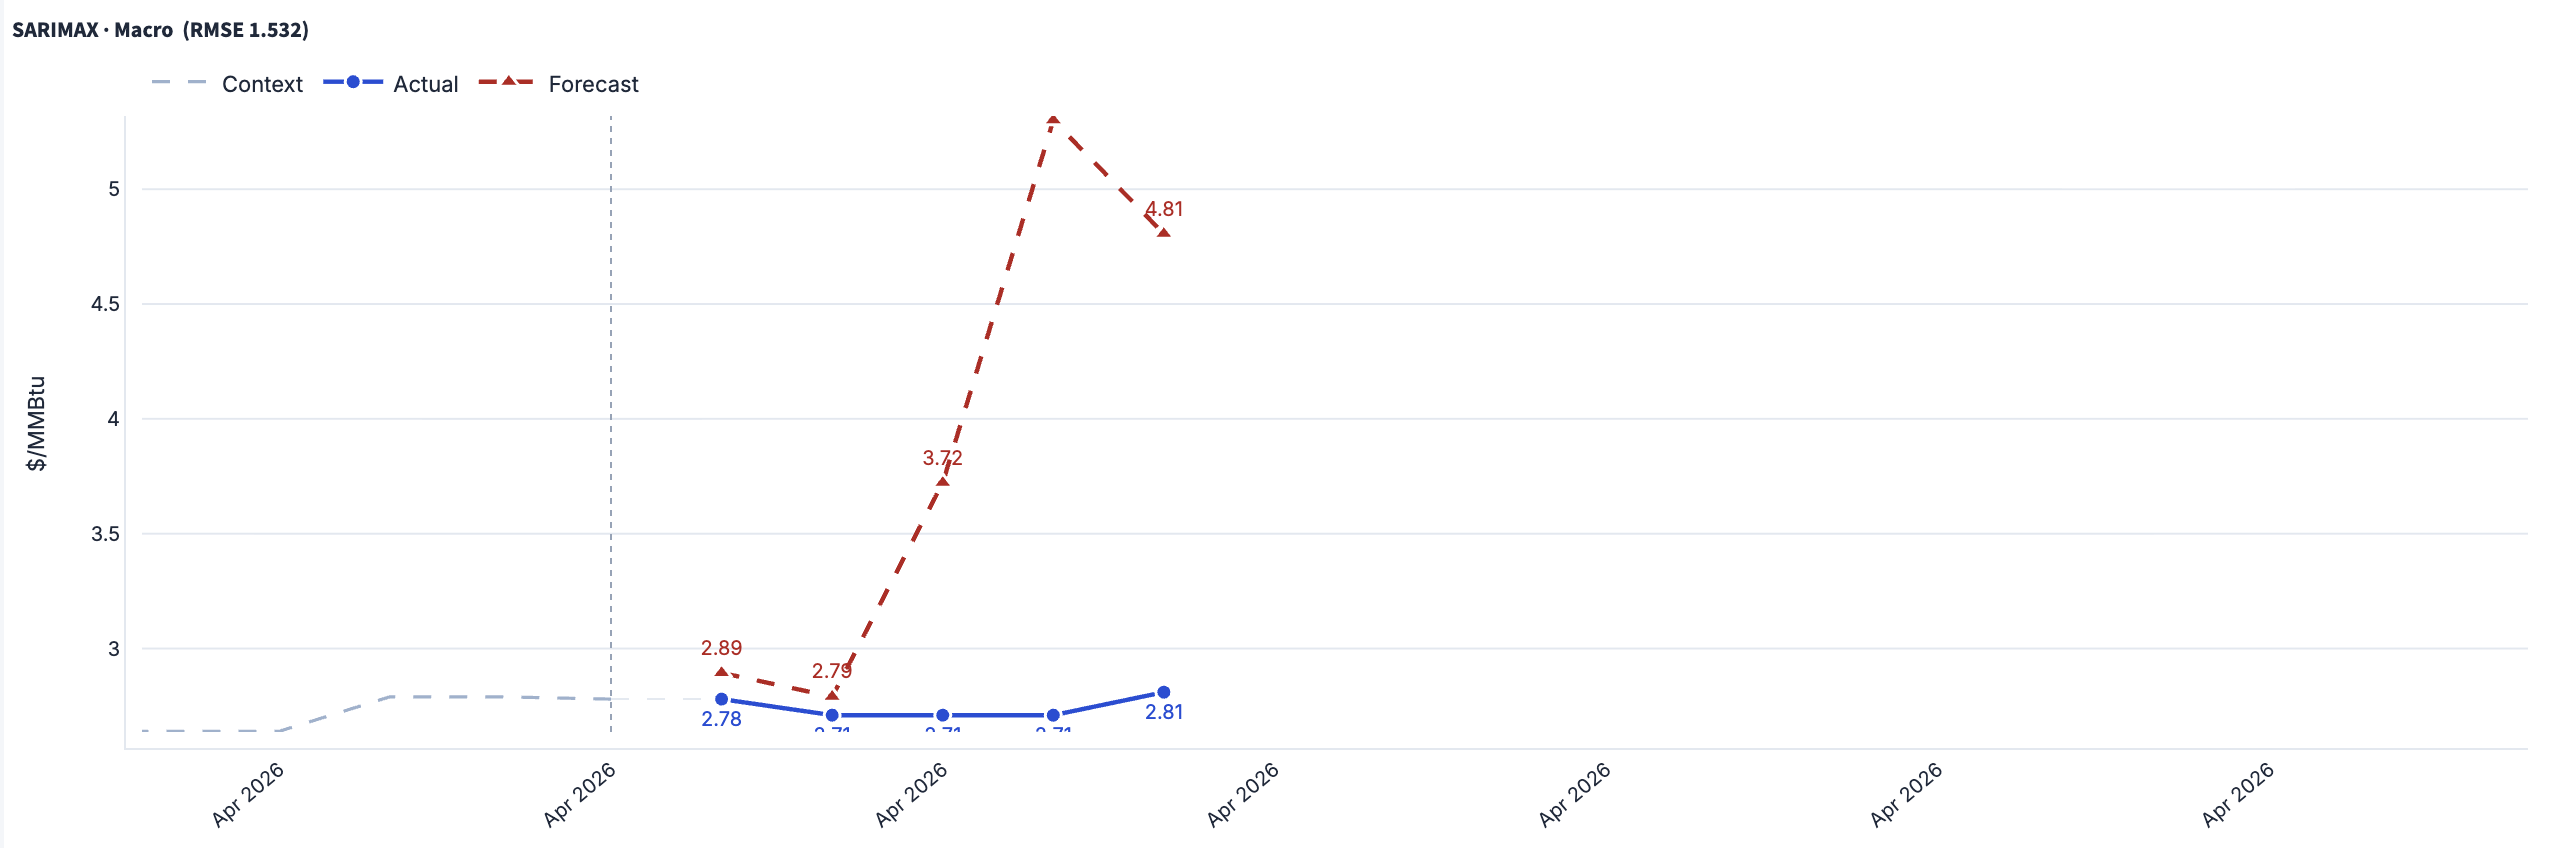
\includegraphics[width=\textwidth]{figures/multivariate_macro_cng_sarimax.png}
\small (a) SARIMAX forecast for natural gas
\end{minipage}\hfill
\begin{minipage}[t]{0.48\textwidth}
\centering
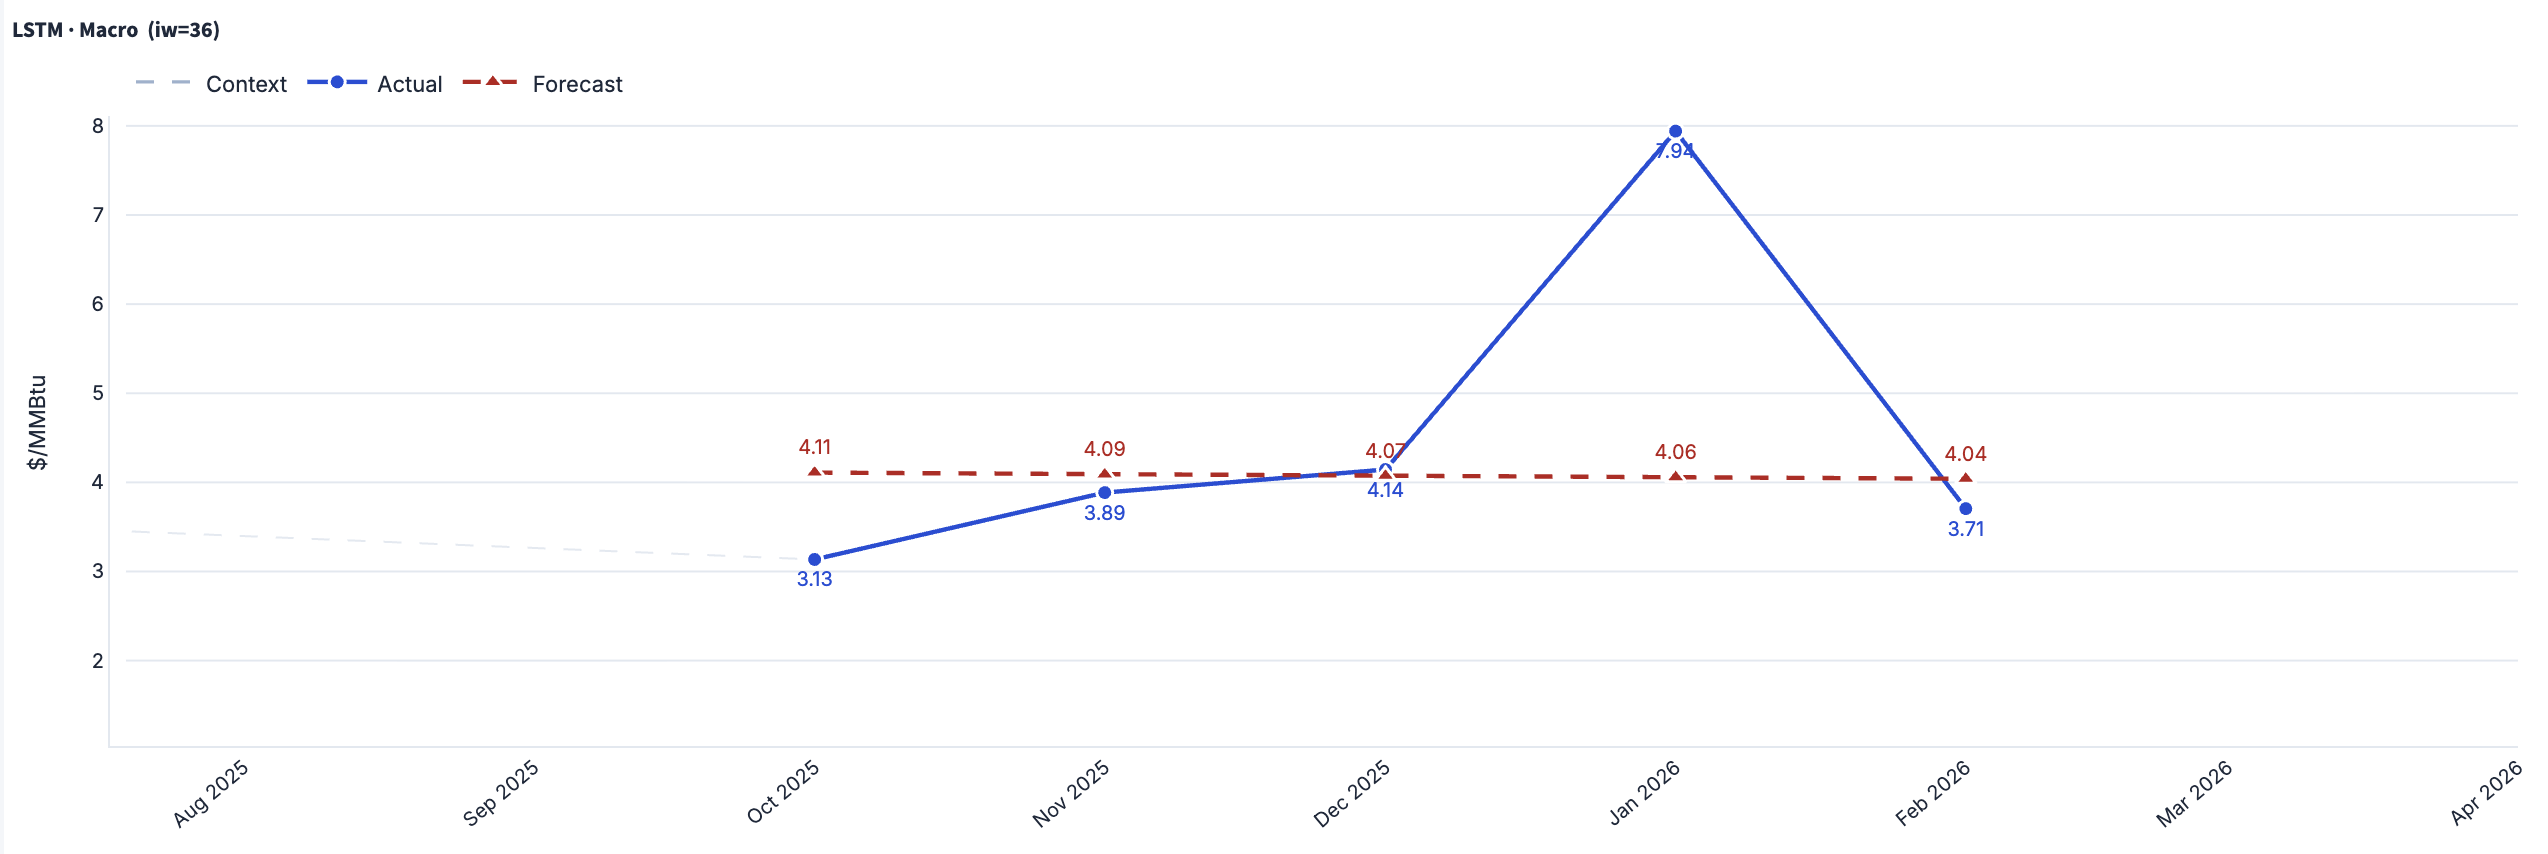
\includegraphics[width=\textwidth]{figures/multivariate_macro_cng_lstm.png}
\small (b) LSTM forecast for natural gas
\end{minipage}

\vspace{0.5em}

\begin{minipage}[t]{0.48\textwidth}
\centering
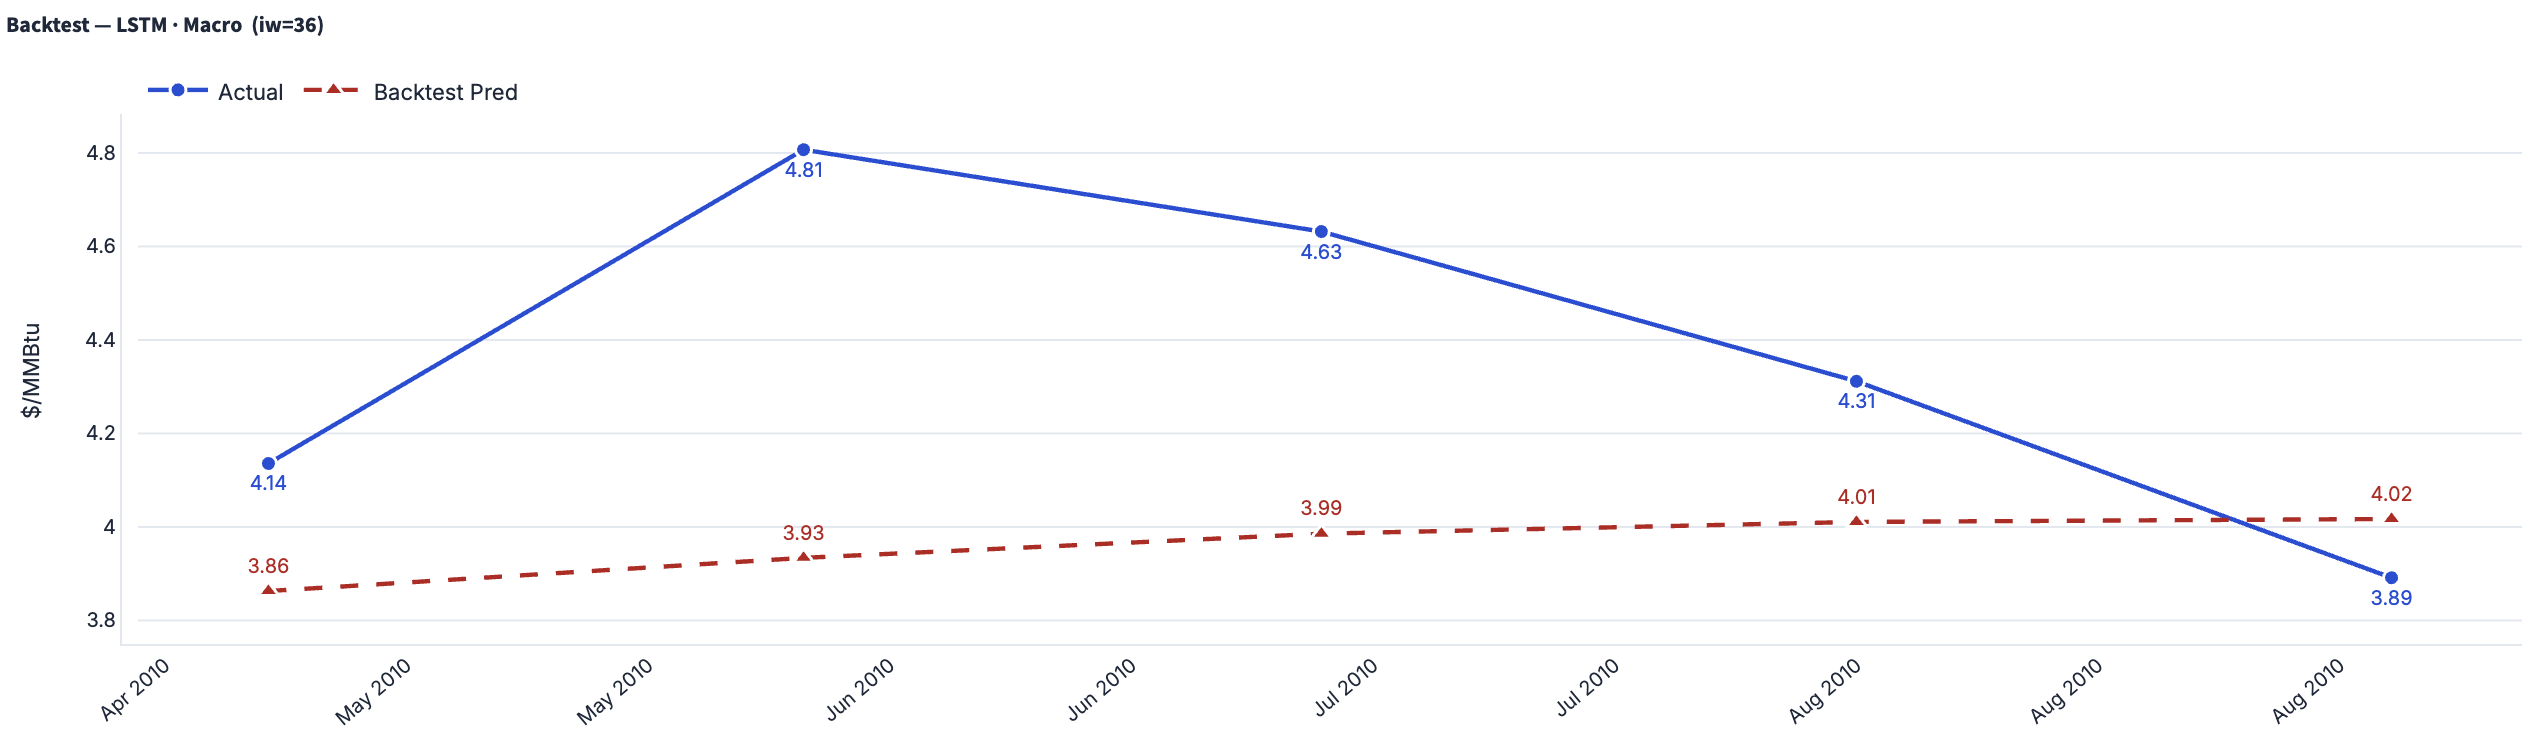
\includegraphics[width=\textwidth]{figures/multivariate_macro_cng_lstm_backtest.png}
\small (c) LSTM backtest for natural gas
\end{minipage}\hfill
\begin{minipage}[t]{0.48\textwidth}
\centering
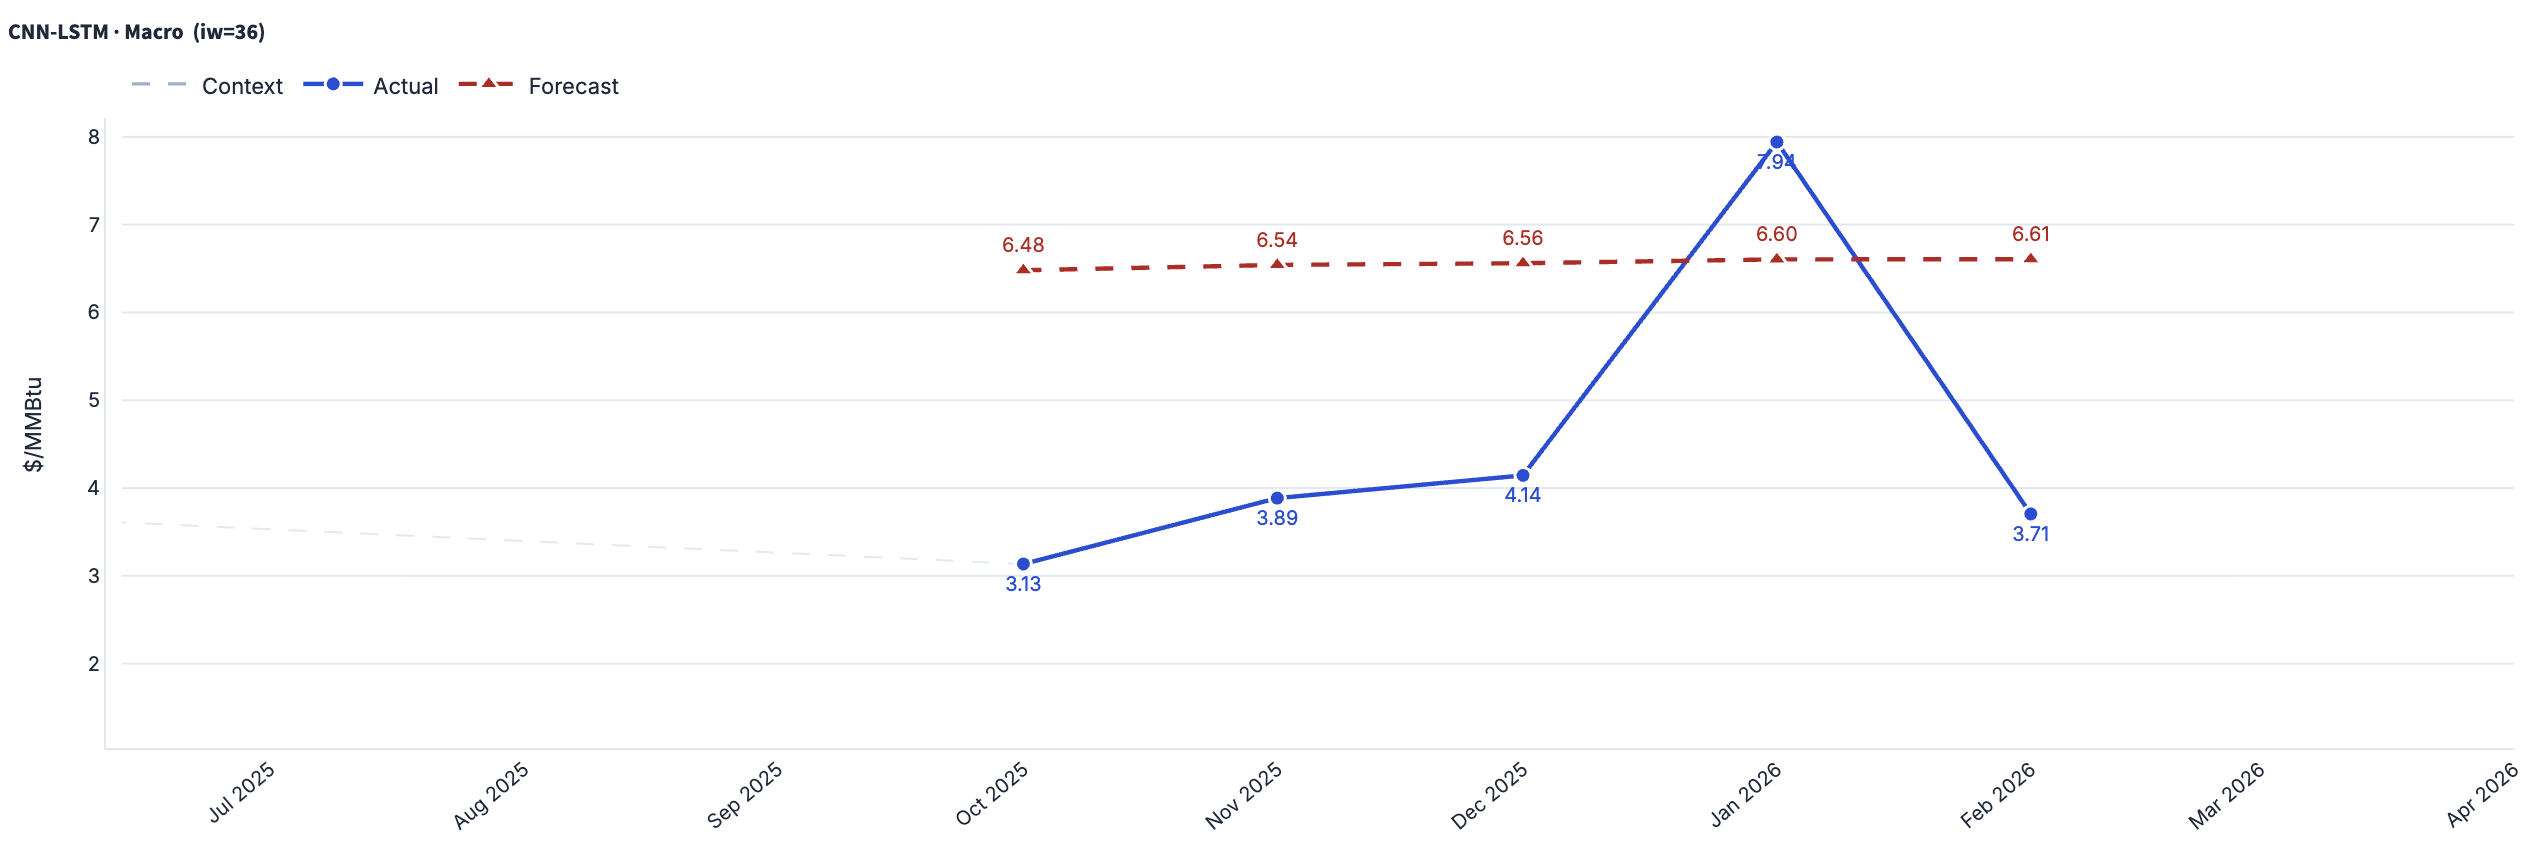
\includegraphics[width=\textwidth]{figures/multivariate_macro_cng_cnnlstm.png}
\small (d) CNN--LSTM forecast for natural gas
\end{minipage}

\vspace{0.5em}

\begin{minipage}[t]{0.48\textwidth}
\centering
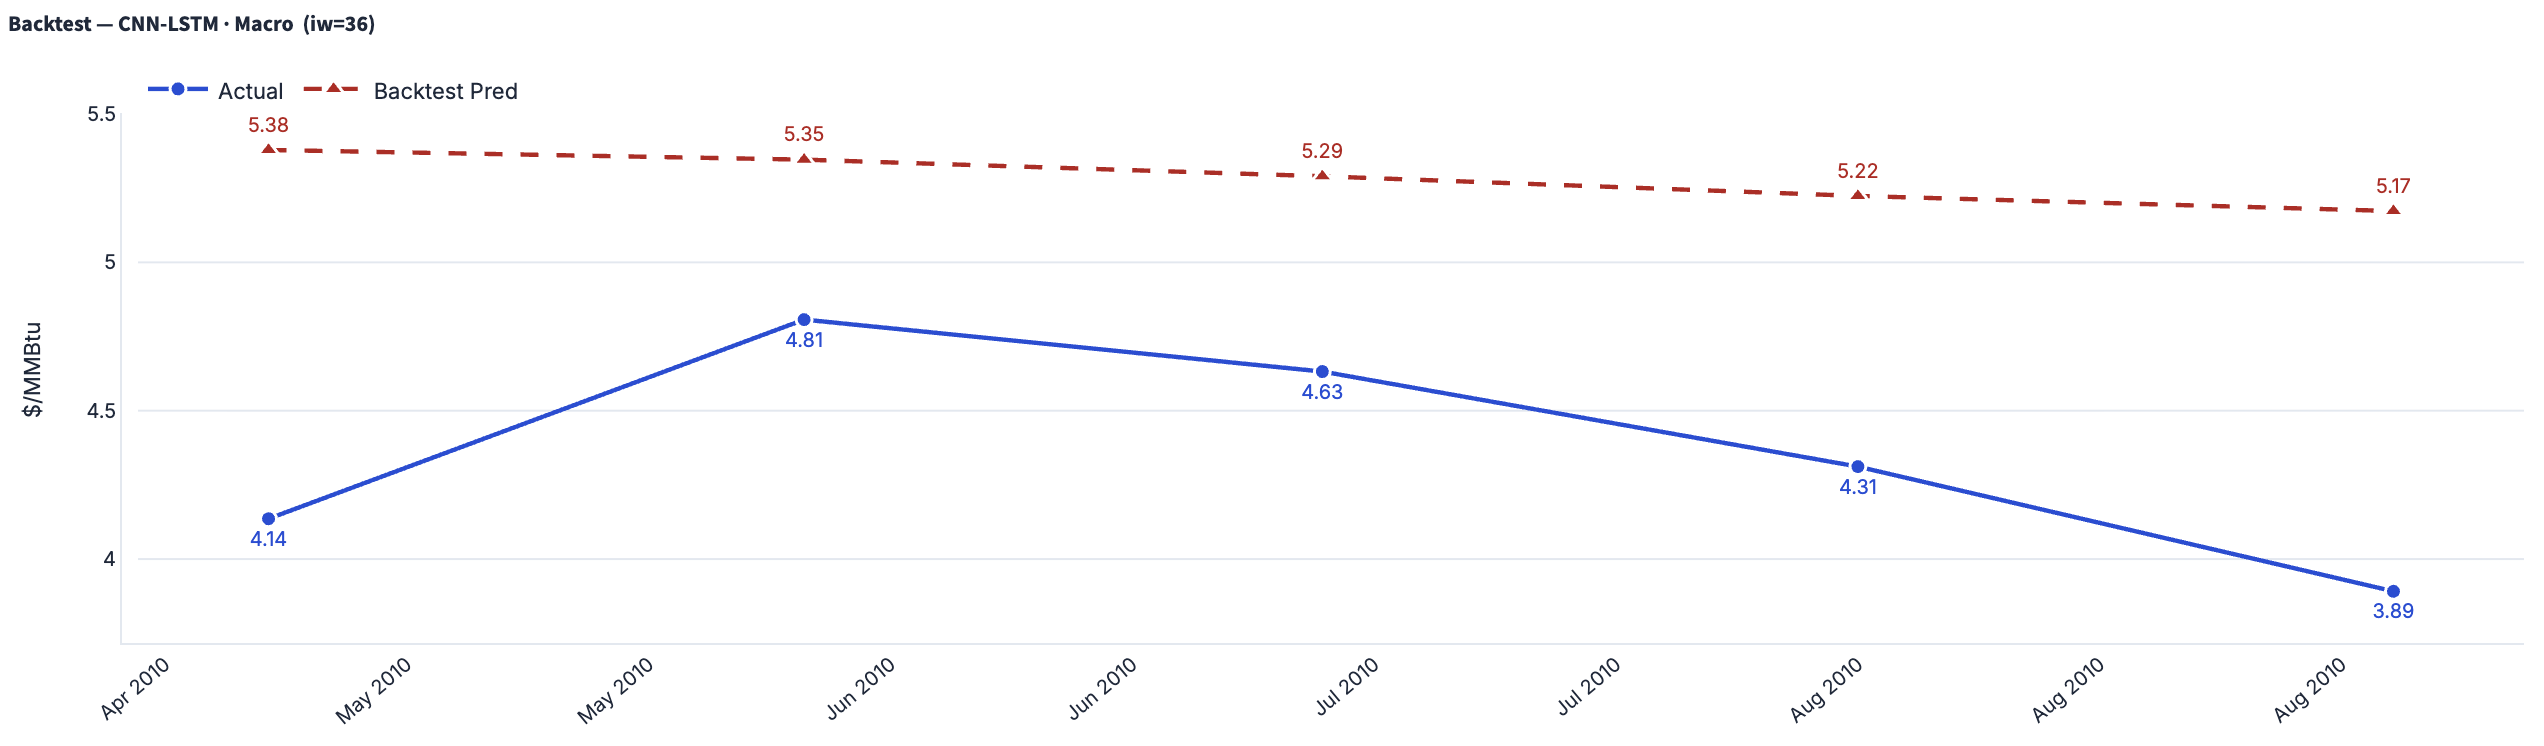
\includegraphics[width=\textwidth]{figures/multivariate_macro_cng_cnnlstm_backtest.png}
\small (e) CNN--LSTM backtest for natural gas
\end{minipage}
\caption{Actual versus predicted Henry Hub natural gas prices (USD/MMBtu) using macroeconomic variables only: (a) SARIMAX forecast with exogenous FRED indicators, (b) LSTM direct forecast, (c) LSTM walk-forward backtest, (d) CNN--LSTM direct forecast, and (e) CNN--LSTM walk-forward backtest. This figure summarizes the macro-only multivariate setting.}
\label{fig:macro_only_cng_plots}
\end{figure}

\begin{table}[h]
\centering
\caption{Macro-only multivariate model performance for natural gas}
\label{tab:macro_only_cng}
\begin{tabular}{@{}lcccc@{}}
\toprule
Model & RMSE (USD/MMBtu) & MAE (USD/MMBtu) & MAPE (\%) & DA \\
\midrule
SARIMAX & 1.532 & 1.158 & 42.20 & 0.20 \\
LSTM Forecast & 1.800 & 1.093 & 19.19 & 0.40 \\
LSTM Backtest & 0.522 & 0.444 & 9.79 & 0.25 \\
CNN--LSTM Forecast & 2.619 & 2.532 & 65.72 & 0.60 \\
CNN--LSTM Backtest & 0.974 & 0.927 & 21.91 & 0.00 \\
\botrule
\end{tabular}
\end{table}

As shown in Figure~\ref{fig:macro_only_cng_plots}, macroeconomic variables alone provide limited predictive capability for natural gas prices. SARIMAX again records relatively high error, indicating that a linear multivariate specification is not sufficient to explain the observed movement in the series. The LSTM model delivers more moderate forecasting performance and comparatively stable backtesting results, suggesting that it models part of the temporal structure, although not strongly enough to track the series consistently.

The CNN--LSTM model performs poorly in direct forecasting despite achieving the highest DA in this setting (0.60), which points to inconsistency in what the model learns across evaluation settings. The LSTM backtest lowers RMSE to 0.522, but its DA remains only 0.25, while the CNN--LSTM backtest drops to 0.00. More broadly, the figure shows that none of the macro-only models are able to follow actual natural gas price movements in a consistently reliable way. Across both crude oil and natural gas, these findings suggest that macroeconomic variables used in isolation are not sufficiently predictive of short-term energy price dynamics. While the neural architectures show some ability to reproduce local patterns, their performance remains unstable across forecasting and backtesting, reinforcing the need to incorporate additional information sources, particularly news-based signals, in the subsequent multivariate settings.

\subsubsection*{5.2.2 News Only}

We designed this setting to evaluate the standalone contribution of news-derived signals. We conducted the experiments using only features extracted from the GDELT dataset, including aggregated event counts, average tone, and the Goldstein scale, which together reflect event-driven and sentiment-based information.

Given the highly dynamic and unstructured nature of news data, we selected the CNN--LSTM architecture for this setting. The convolutional component models local temporal patterns across event features, while the LSTM layer models sequential dependencies over time. For crude oil, the model was trained using an input window of 24 time steps and a multi-step output of 5 steps in a one-shot forecasting setting. For natural gas, an input window of 36 time steps with a single-step output was used.

\subsubsection*{5.2.2.1 Crude Oil}
For crude oil, Table~\ref{tab:news_only_oil} summarizes the performance of the news-only CNN--LSTM model, and Figure~\ref{fig:news_only_oil_plots} shows the corresponding forecast and backtest plots.

\begin{figure}[h]
\centering
\begin{minipage}[t]{0.48\textwidth}
\centering
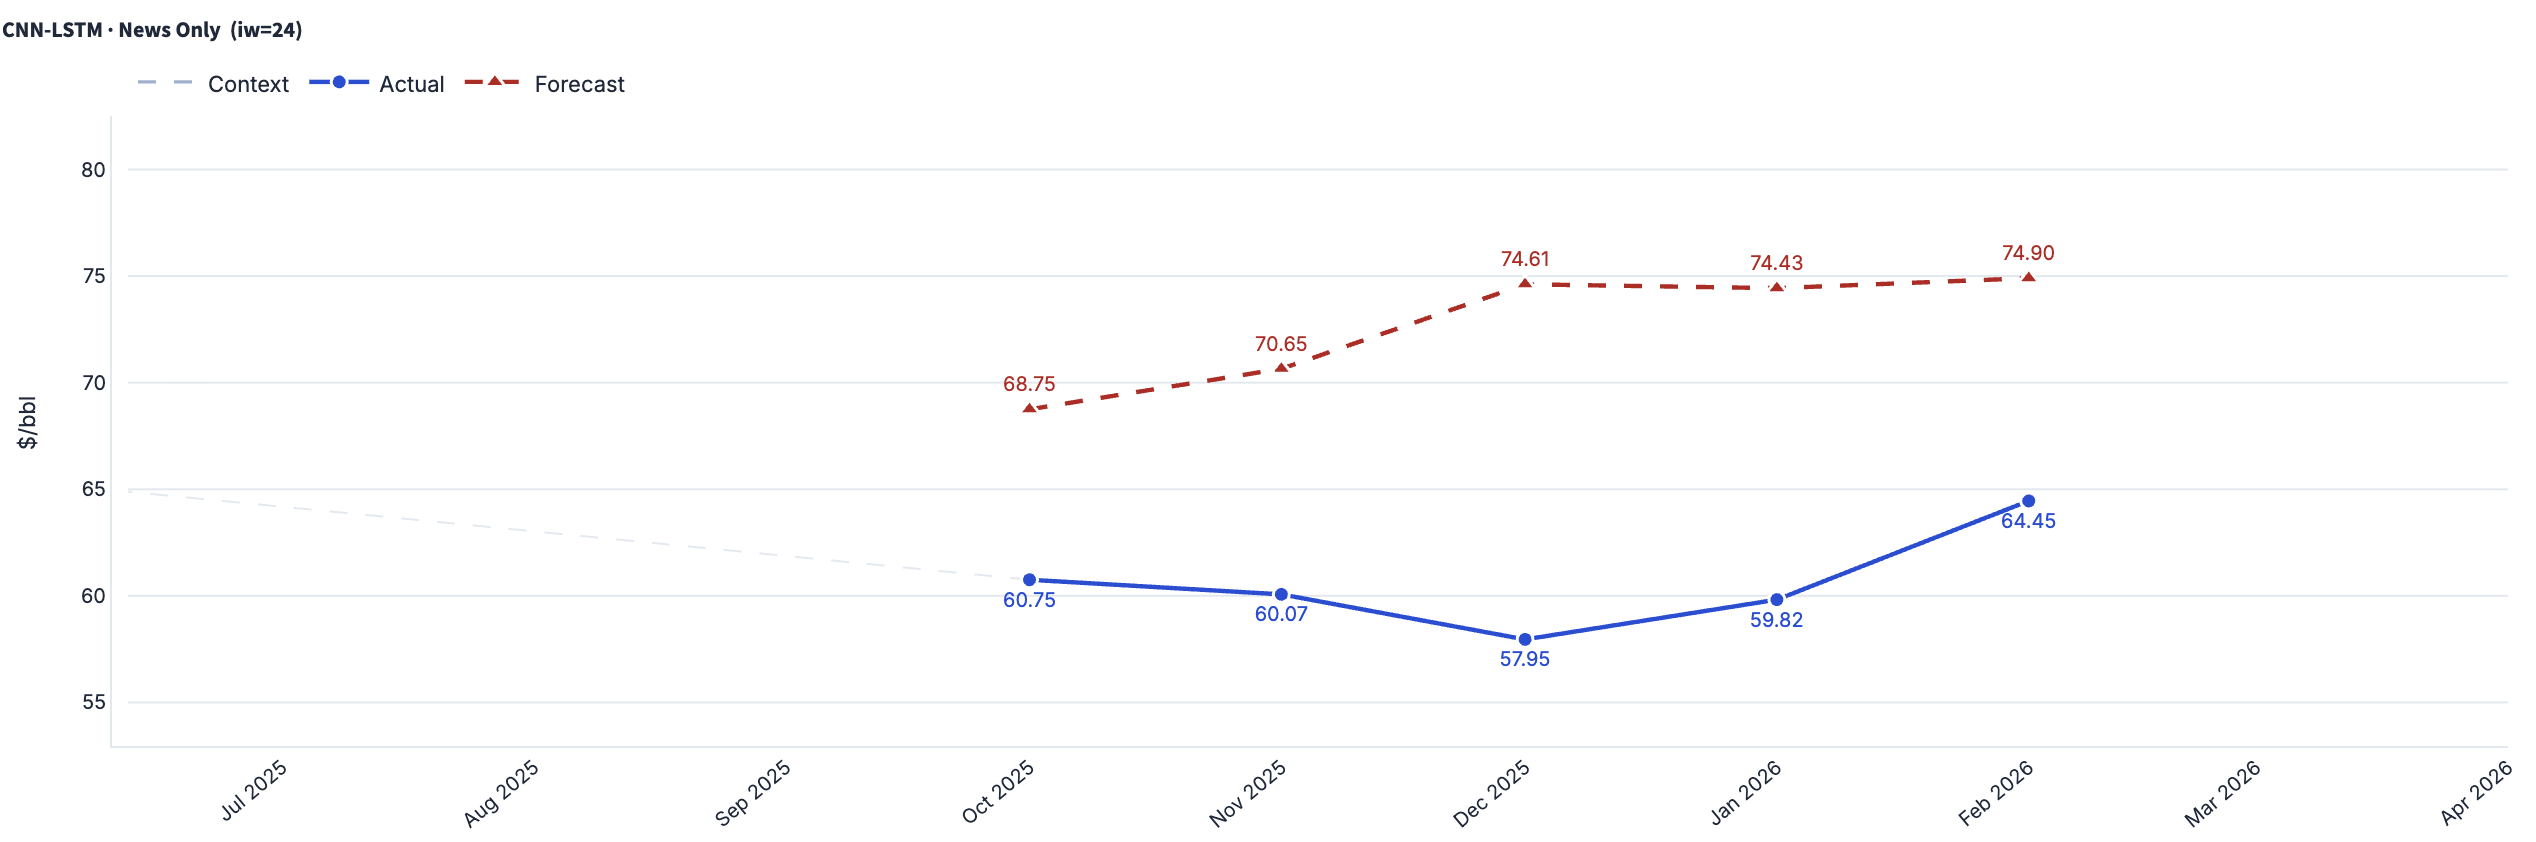
\includegraphics[width=\textwidth]{figures/multivariate_oil_news_cnn_lstm.png}
\small (a) CNN--LSTM forecast for crude oil using news features
\end{minipage}\hfill
\begin{minipage}[t]{0.48\textwidth}
\centering
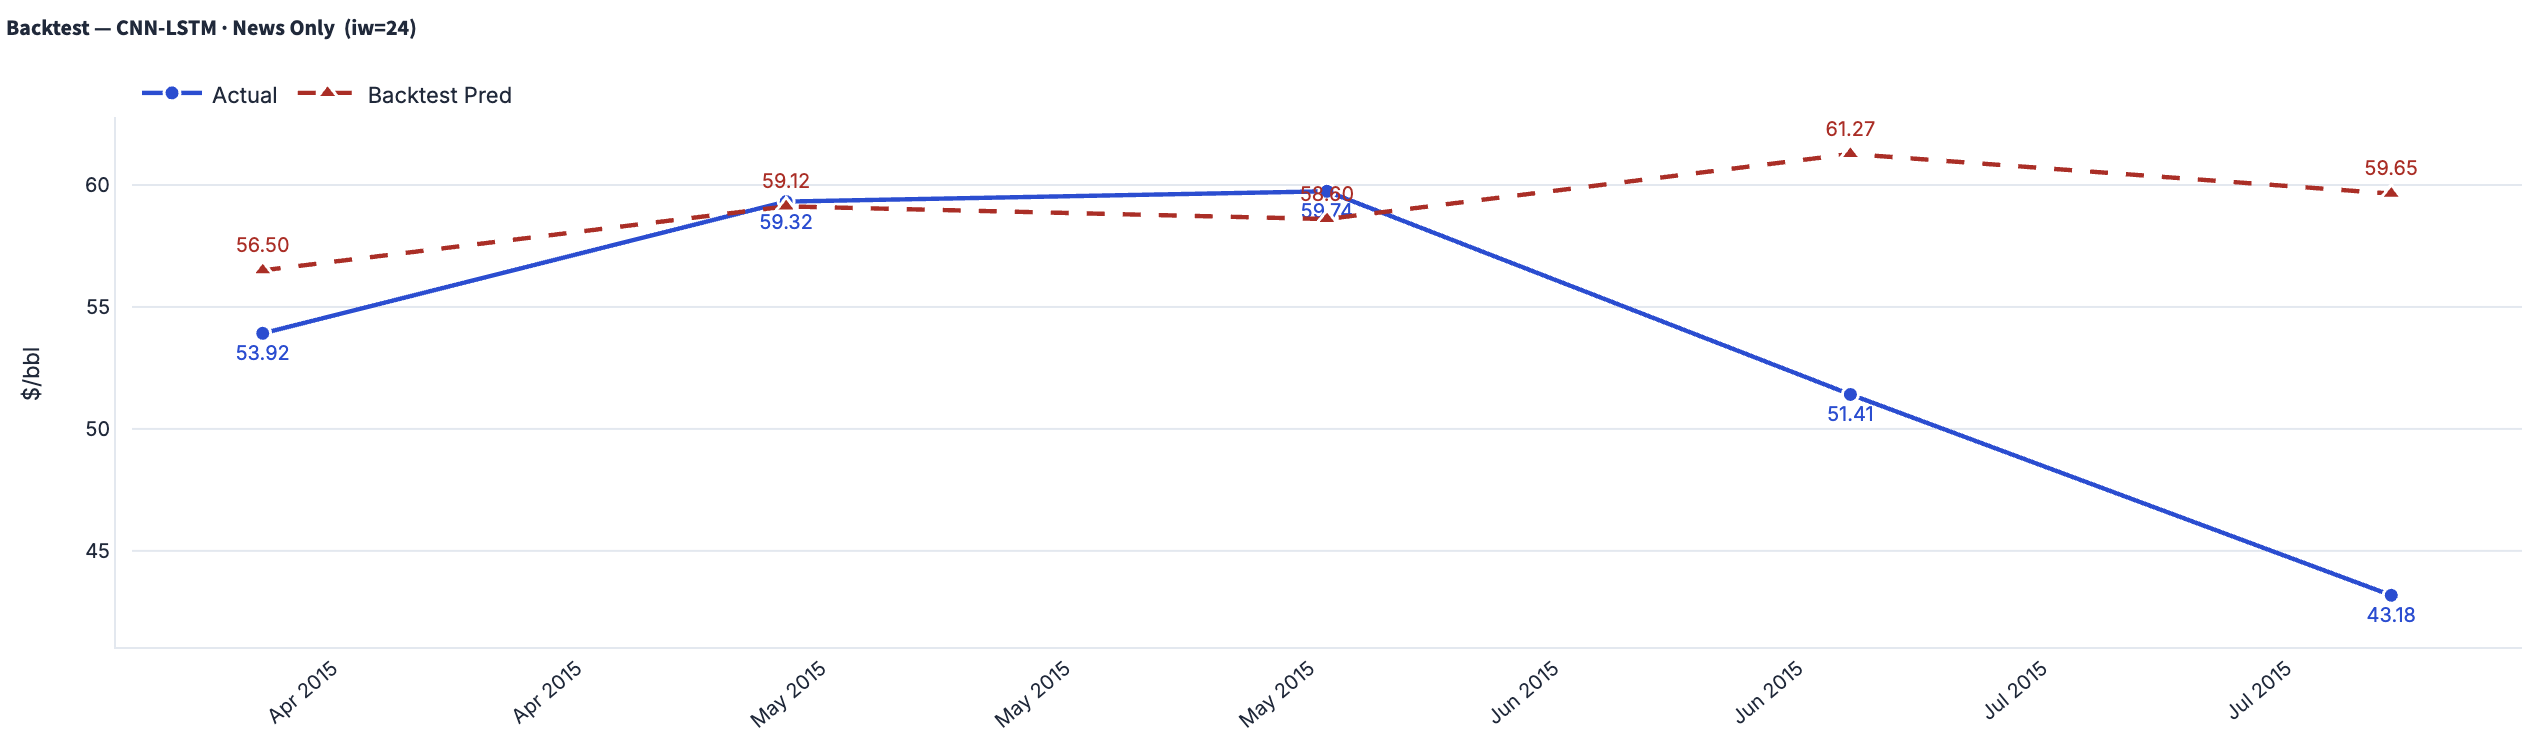
\includegraphics[width=\textwidth]{figures/multivariate_oil_news_cnn_lstm_backtest.png}
\small (b) CNN--LSTM backtest for crude oil using news features
\end{minipage}
\caption{Actual versus predicted WTI crude oil prices (USD/barrel) using only GDELT-derived news features in the CNN--LSTM setting: (a) direct forecast and (b) walk-forward backtest. The panels summarize the standalone contribution of event-count, tone, and Goldstein-scale signals without macroeconomic inputs.}
\label{fig:news_only_oil_plots}
\end{figure}

\begin{table}[h]
\centering
\caption{News-only model performance for crude oil}
\label{tab:news_only_oil}
\begin{tabular}{@{}lcccc@{}}
\toprule
Model & RMSE (USD/barrel) & MAE (USD/barrel) & MAPE (\%) & DA \\
\midrule
CNN--LSTM Forecast & 12.459 & 12.060 & 20.03 & 0.60 \\
CNN--LSTM Backtest & 8.676 & 6.049 & 12.87 & 0.40 \\
\botrule
\end{tabular}
\end{table}

Figure~\ref{fig:news_only_oil_plots} indicates that the news-only CNN--LSTM model is able to track some variation in crude oil prices, suggesting that event-driven signals do contain useful information. However, the forecasting errors remain relatively high, and the model does not align consistently with the observed price path. The forecast tracks the broad direction of movement in some periods, but it struggles to match sharp fluctuations and exact price levels.

The backtesting results show moderate improvement relative to the direct forecast, but the error remains large enough to suggest that the model is not sufficiently reliable on its own. In directional terms, the forecast DA of 0.60 is stronger than the backtest DA of 0.40, indicating that the news-only model captures some broad sign changes for crude oil but cannot do so consistently across rolling windows. In substantive terms, the figure shows a model that can reflect general market shifts associated with news flow, yet lacks the precision needed for dependable short-term forecasting. This suggests that while news-derived signals carry relevant information for crude oil, they are not strong enough in isolation to fully explain the dynamics of the series.

\subsubsection*{5.2.2.2 Natural Gas (CNG)}
For natural gas, Table~\ref{tab:news_only_cng} reports the news-only CNN--LSTM results, and Figure~\ref{fig:news_only_cng_plots} illustrates them.

\begin{figure}[h]
\centering
\begin{minipage}[t]{0.48\textwidth}
\centering
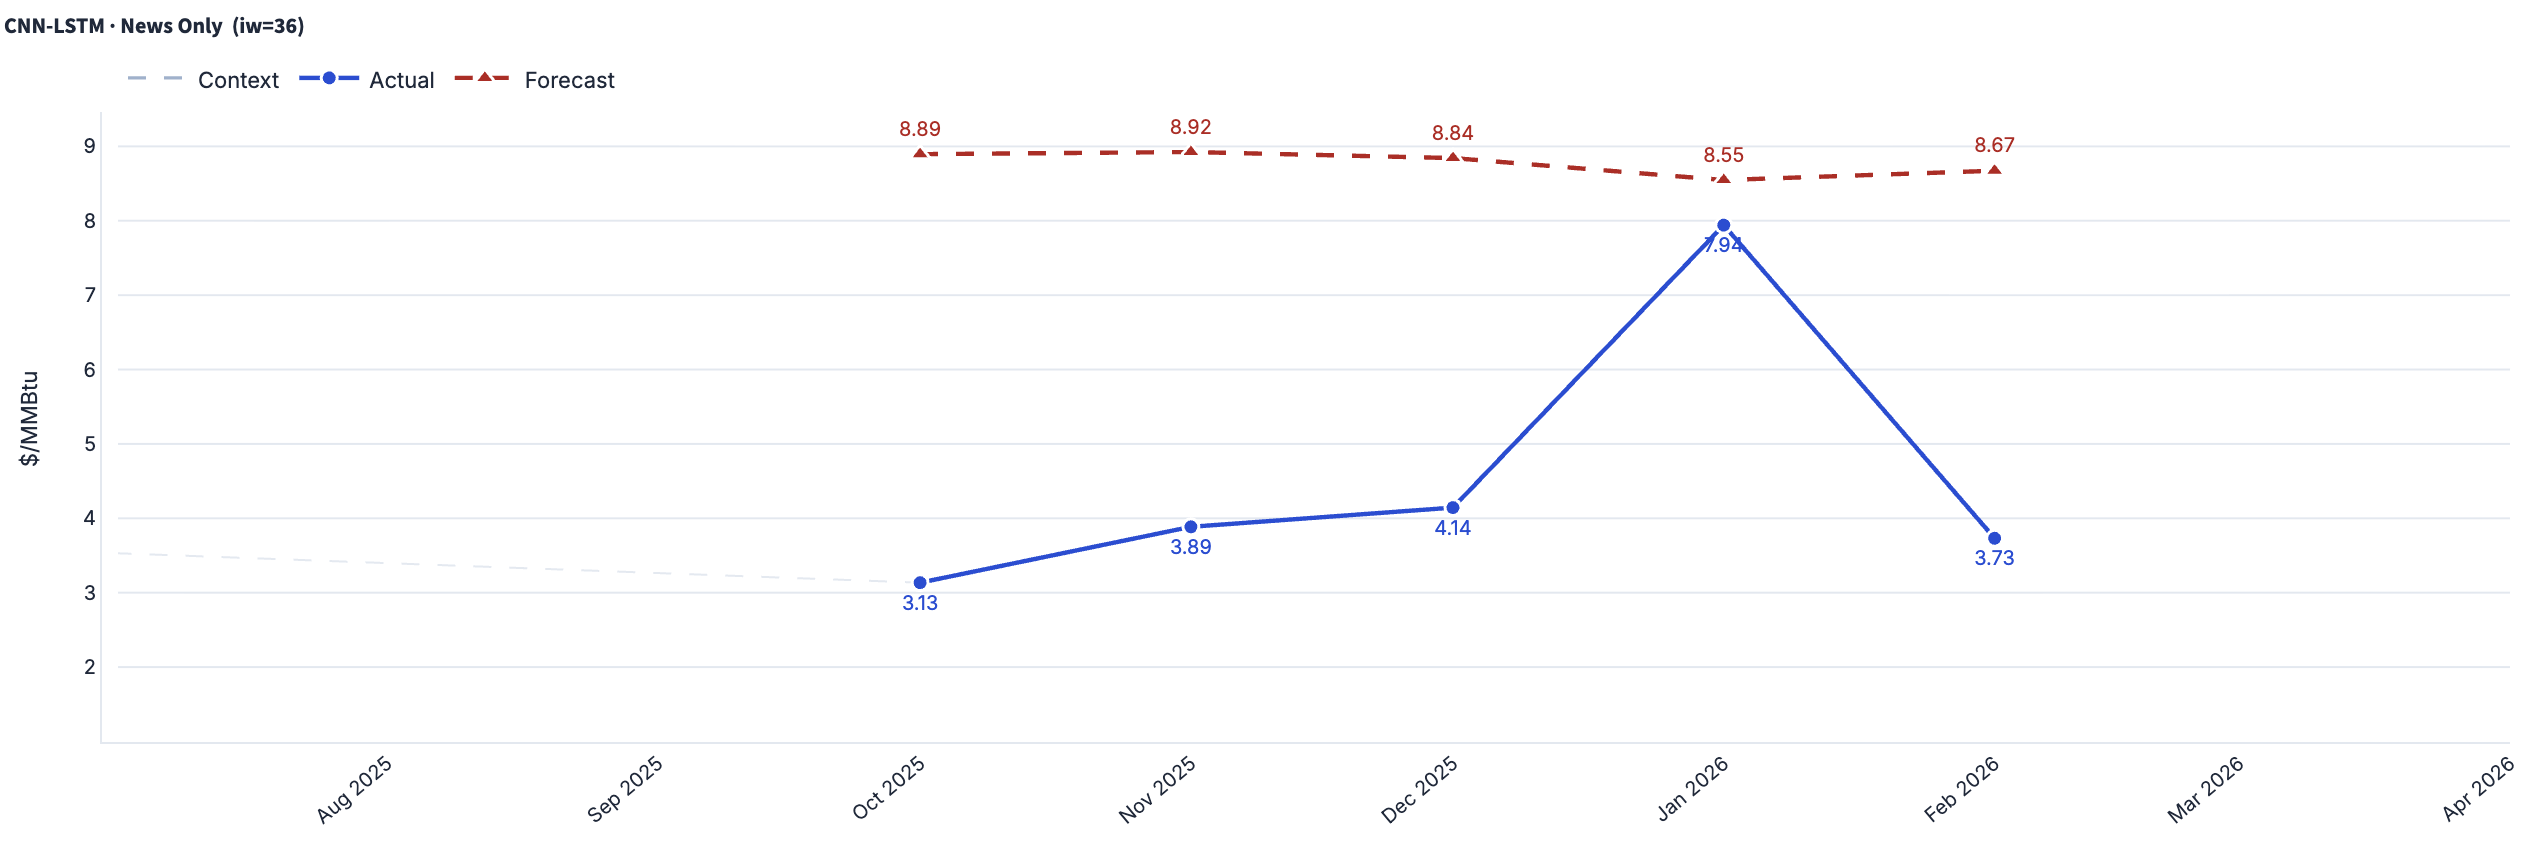
\includegraphics[width=\textwidth]{figures/multivariate_cng_news_cnn_lstm.png}
\small (a) CNN--LSTM forecast for natural gas using news features
\end{minipage}\hfill
\begin{minipage}[t]{0.48\textwidth}
\centering
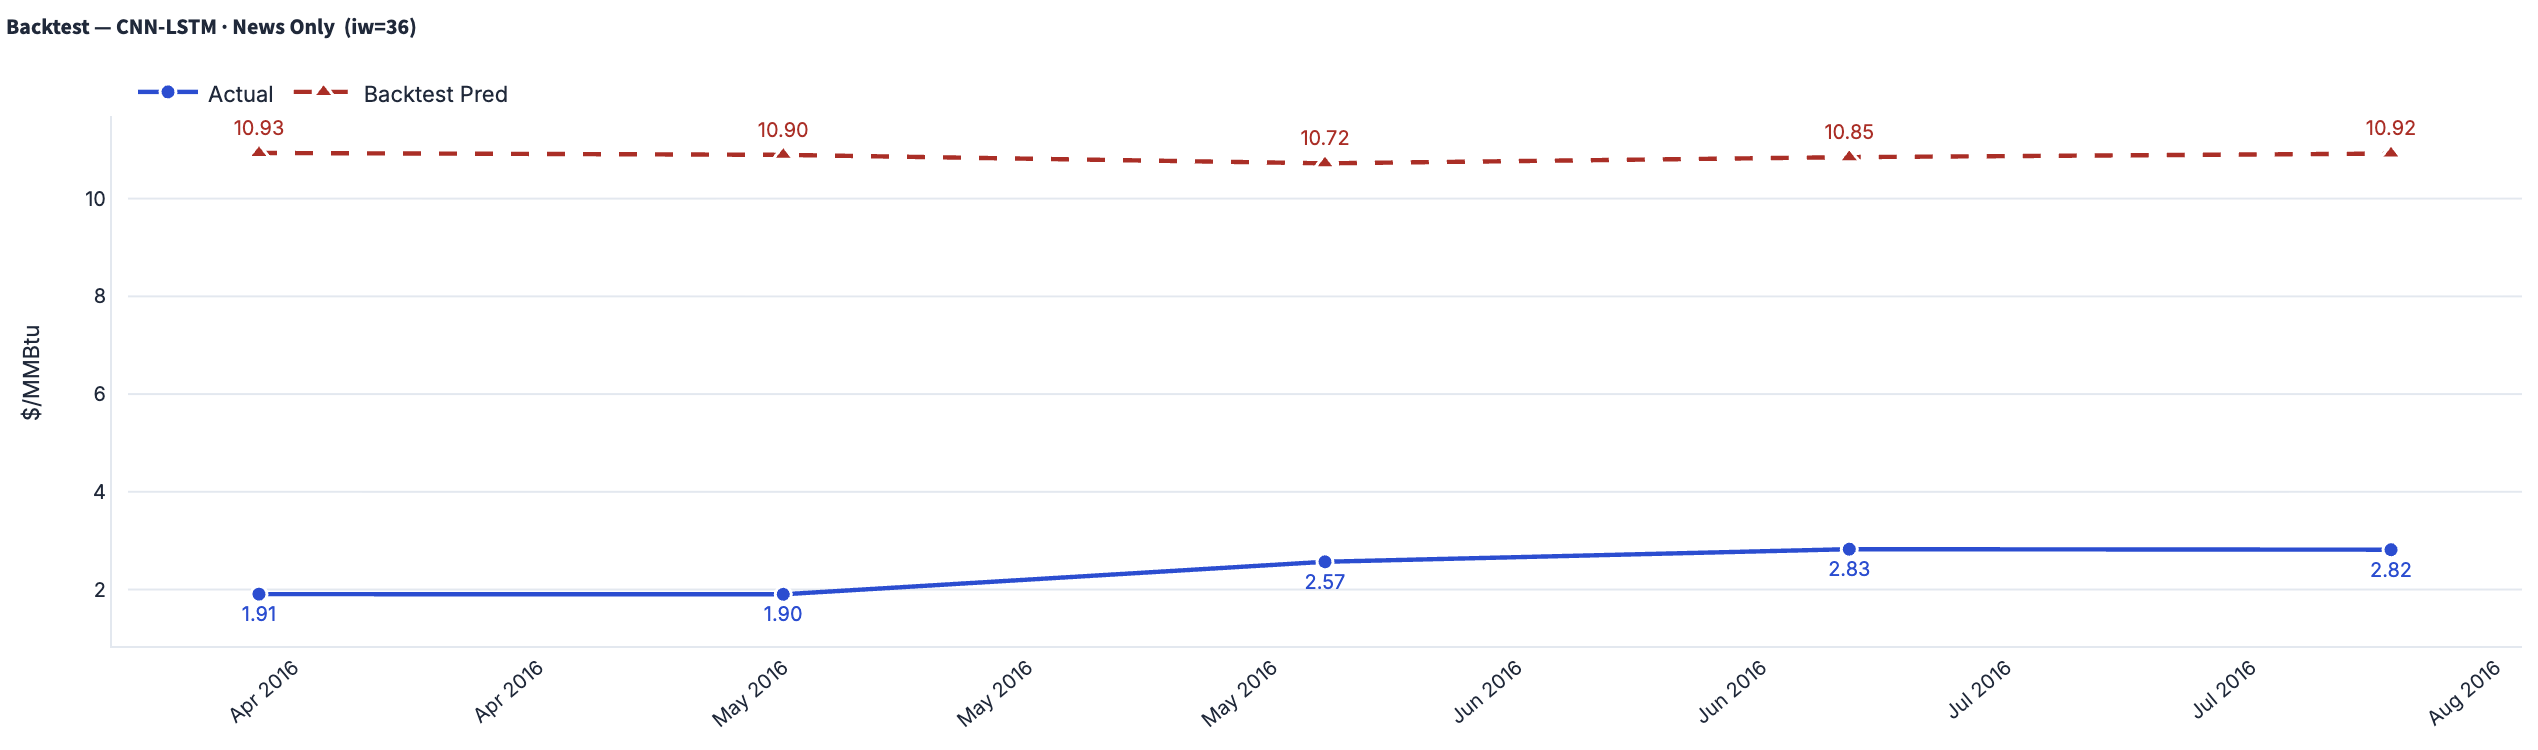
\includegraphics[width=\textwidth]{figures/multivariate_cng_news_cnn_lstm_backtest.png}
\small (b) CNN--LSTM backtest for natural gas using news features
\end{minipage}
\caption{Actual versus predicted Henry Hub natural gas prices (USD/MMBtu) using only GDELT-derived news features in the CNN--LSTM setting: (a) direct forecast and (b) walk-forward backtest. The panels summarize the standalone contribution of event-count, tone, and Goldstein-scale signals without macroeconomic inputs.}
\label{fig:news_only_cng_plots}
\end{figure}

\begin{table}[h]
\centering
\caption{News-only model performance for natural gas}
\label{tab:news_only_cng}
\begin{tabular}{@{}lcccc@{}}
\toprule
Model & RMSE (USD/MMBtu) & MAE (USD/MMBtu) & MAPE (\%) & DA \\
\midrule
CNN--LSTM Forecast & 4.592 & 4.209 & 113.37 & 0.40 \\
CNN--LSTM Backtest & 8.473 & 8.461 & 367.16 & 0.00 \\
\botrule
\end{tabular}
\end{table}

As shown in Figure~\ref{fig:news_only_cng_plots}, the performance of the news-only model for natural gas is substantially weaker than for crude oil. Both forecasting and backtesting errors are high, indicating that news-derived features alone are insufficient to explain natural gas price movements in a stable or accurate way. The predictions deviate markedly from the observed series and fail to reproduce both the direction and magnitude of many changes. The DA results confirm this weakness, dropping from 0.40 in the direct forecast to 0.00 in backtesting.

This pattern suggests that, for natural gas, the information contained in aggregated news signals is too indirect or too noisy to support reliable standalone forecasting. Compared with crude oil, where news appears to offer at least some useful directional information, the CNG results point to a much weaker connection between the extracted GDELT features and short-term price behavior.

Taken together, the news-only results show that event-driven signals are informative but not sufficient on their own for robust energy price forecasting. For crude oil, the CNN--LSTM model tracks broad movements but lacks precision. For natural gas, performance is considerably weaker, indicating that news signals alone do not adequately represent the underlying price dynamics. These findings suggest that news-based features are more useful as complementary inputs than as standalone predictors, and they motivate the combined macro-plus-news setting examined next.

\subsubsection*{5.2.3 Macro + News Combined Model}

To address the limitations observed in the macro-only and news-only settings, both feature groups were combined in a unified multivariate framework. Macroeconomic variables provide structured long-term trends, while news-derived features introduce event-driven and sentiment-based dynamics. By integrating these two sources, we intend the combined setup to reflect complementary information that neither group can provide on its own.

We evaluated this framework using SARIMAX, LSTM, and CNN--LSTM models. For the neural architectures, the sequence configurations were defined as follows: for crude oil, LSTM used a 24-step input and 5-step output, while CNN--LSTM used a 36-step input and 5-step output; for natural gas, both LSTM and CNN--LSTM used a 36-step input and 5-step output. SARIMAX was implemented with monthly modeling for crude oil and daily modeling for natural gas.

\subsubsection*{5.2.3.1 Crude Oil}
Table~\ref{tab:combined_oil} summarizes the performance of the combined-feature models for crude oil, and Figure~\ref{fig:combined_oil_plots} presents the corresponding prediction plots.

\begin{figure}[h]
\centering
\begin{minipage}[t]{0.48\textwidth}
\centering
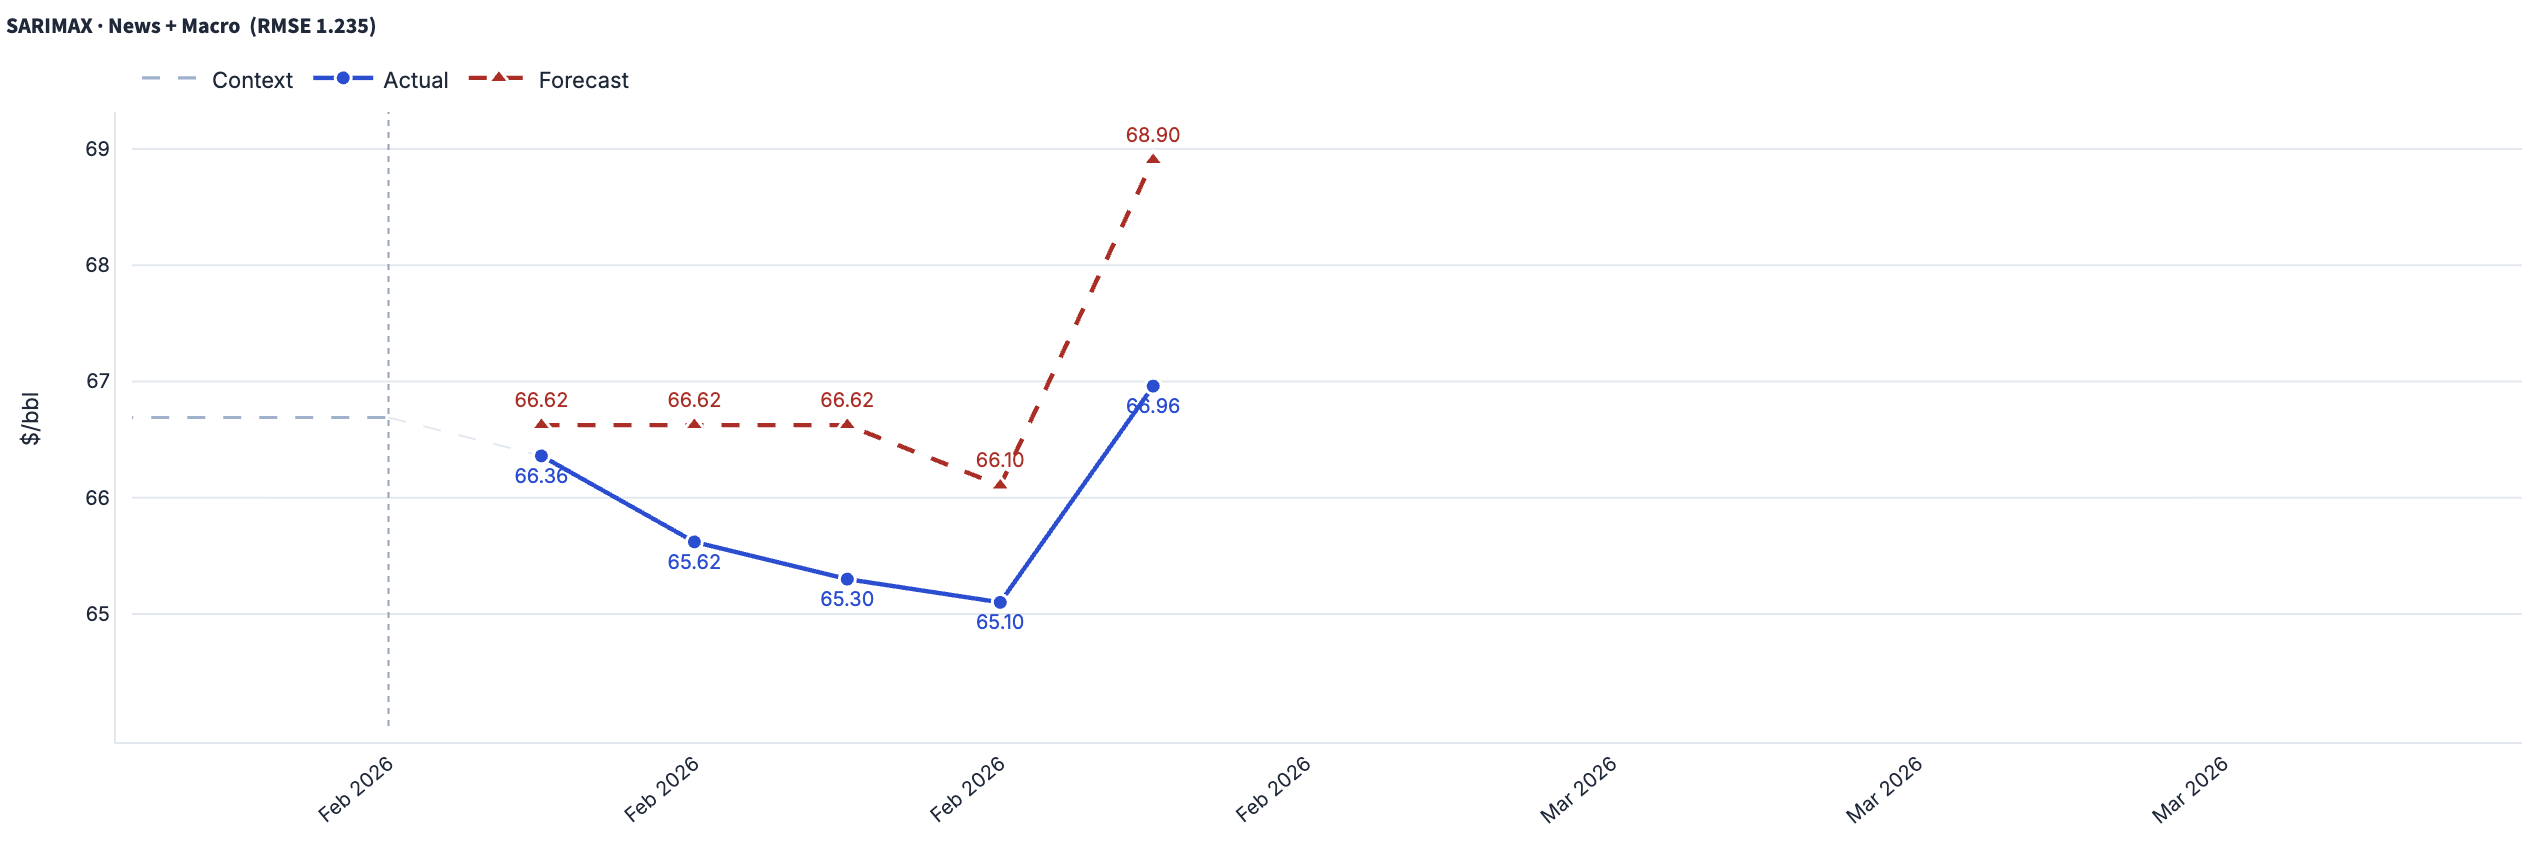
\includegraphics[width=\textwidth]{figures/multivariate_news_macro_oil_sarimax.png}
\small (a) SARIMAX forecast for crude oil
\end{minipage}\hfill
\begin{minipage}[t]{0.48\textwidth}
\centering
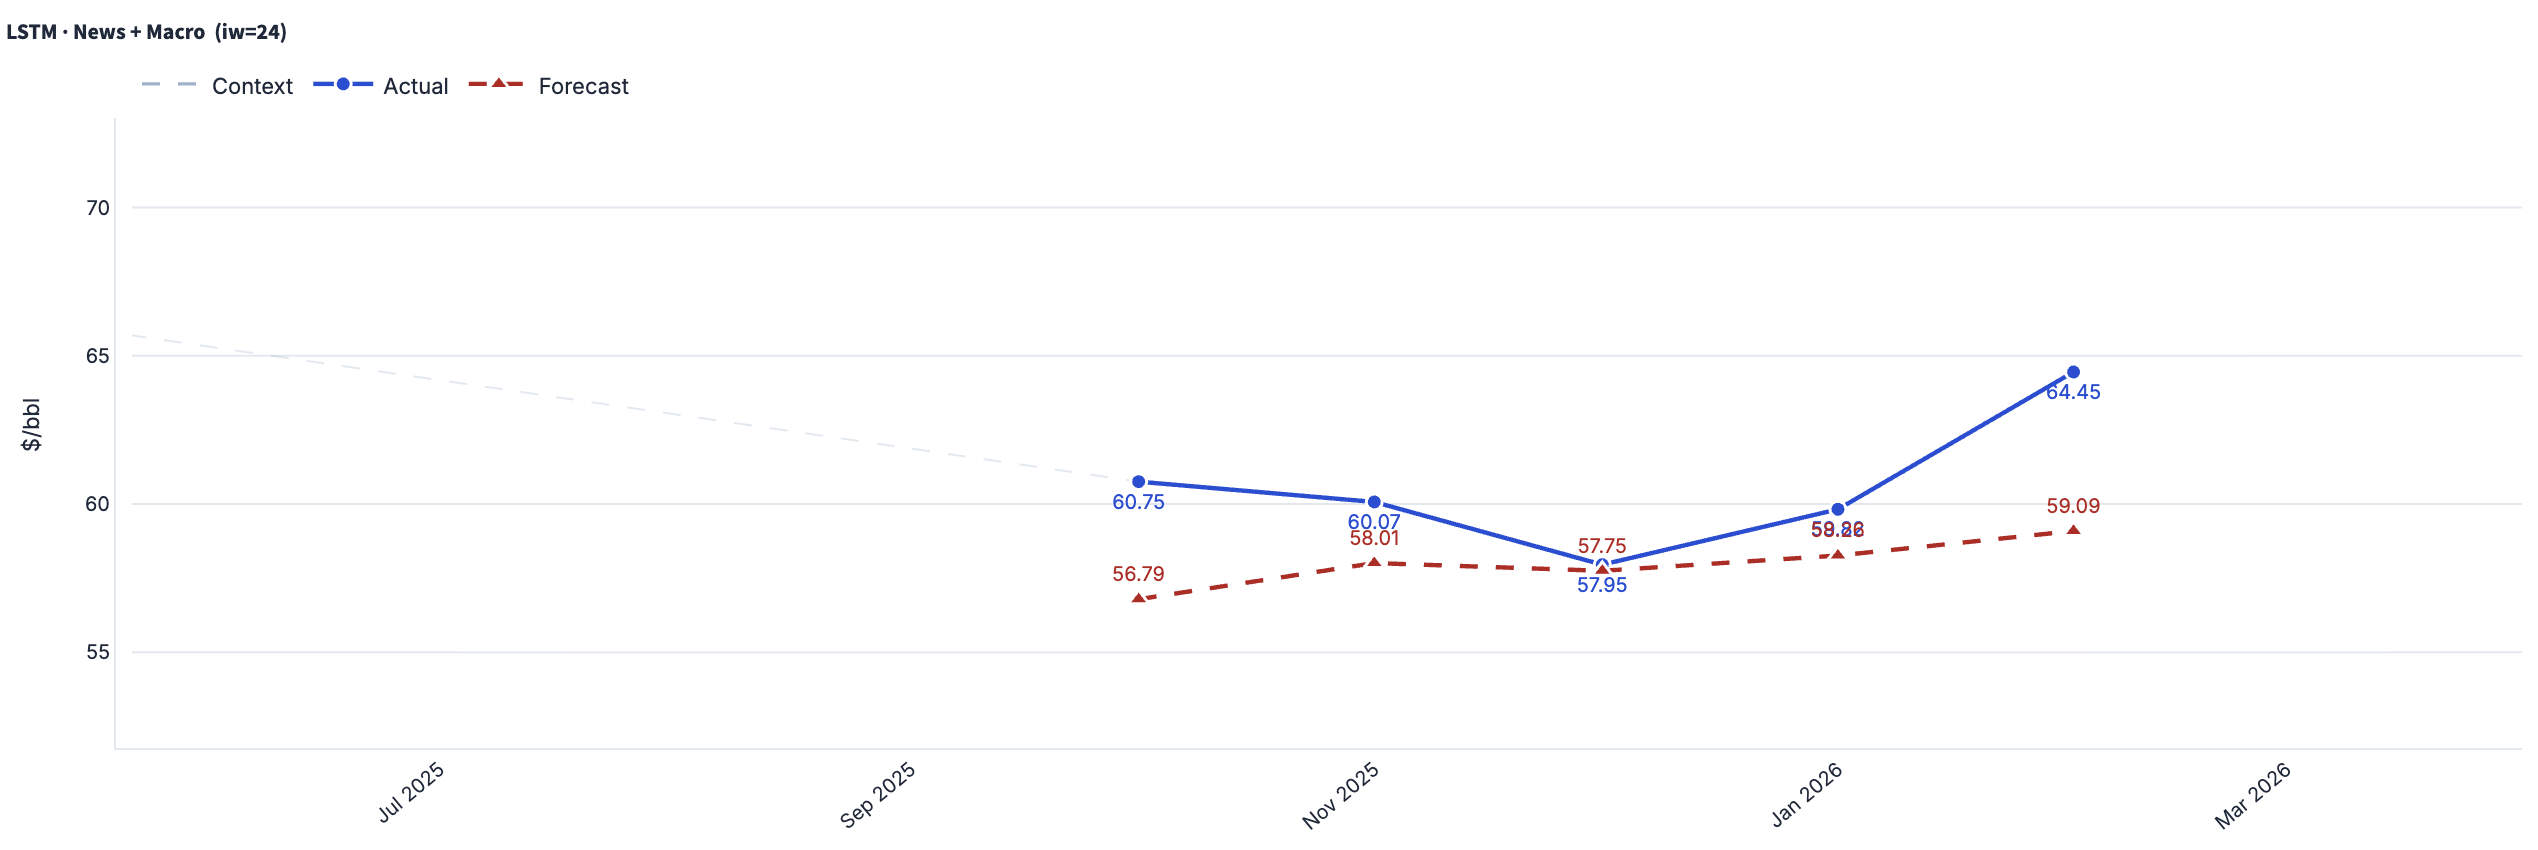
\includegraphics[width=\textwidth]{figures/multivariate_news_macro_oil_lstm.png}
\small (b) LSTM forecast for crude oil
\end{minipage}

\vspace{0.5em}

\begin{minipage}[t]{0.48\textwidth}
\centering
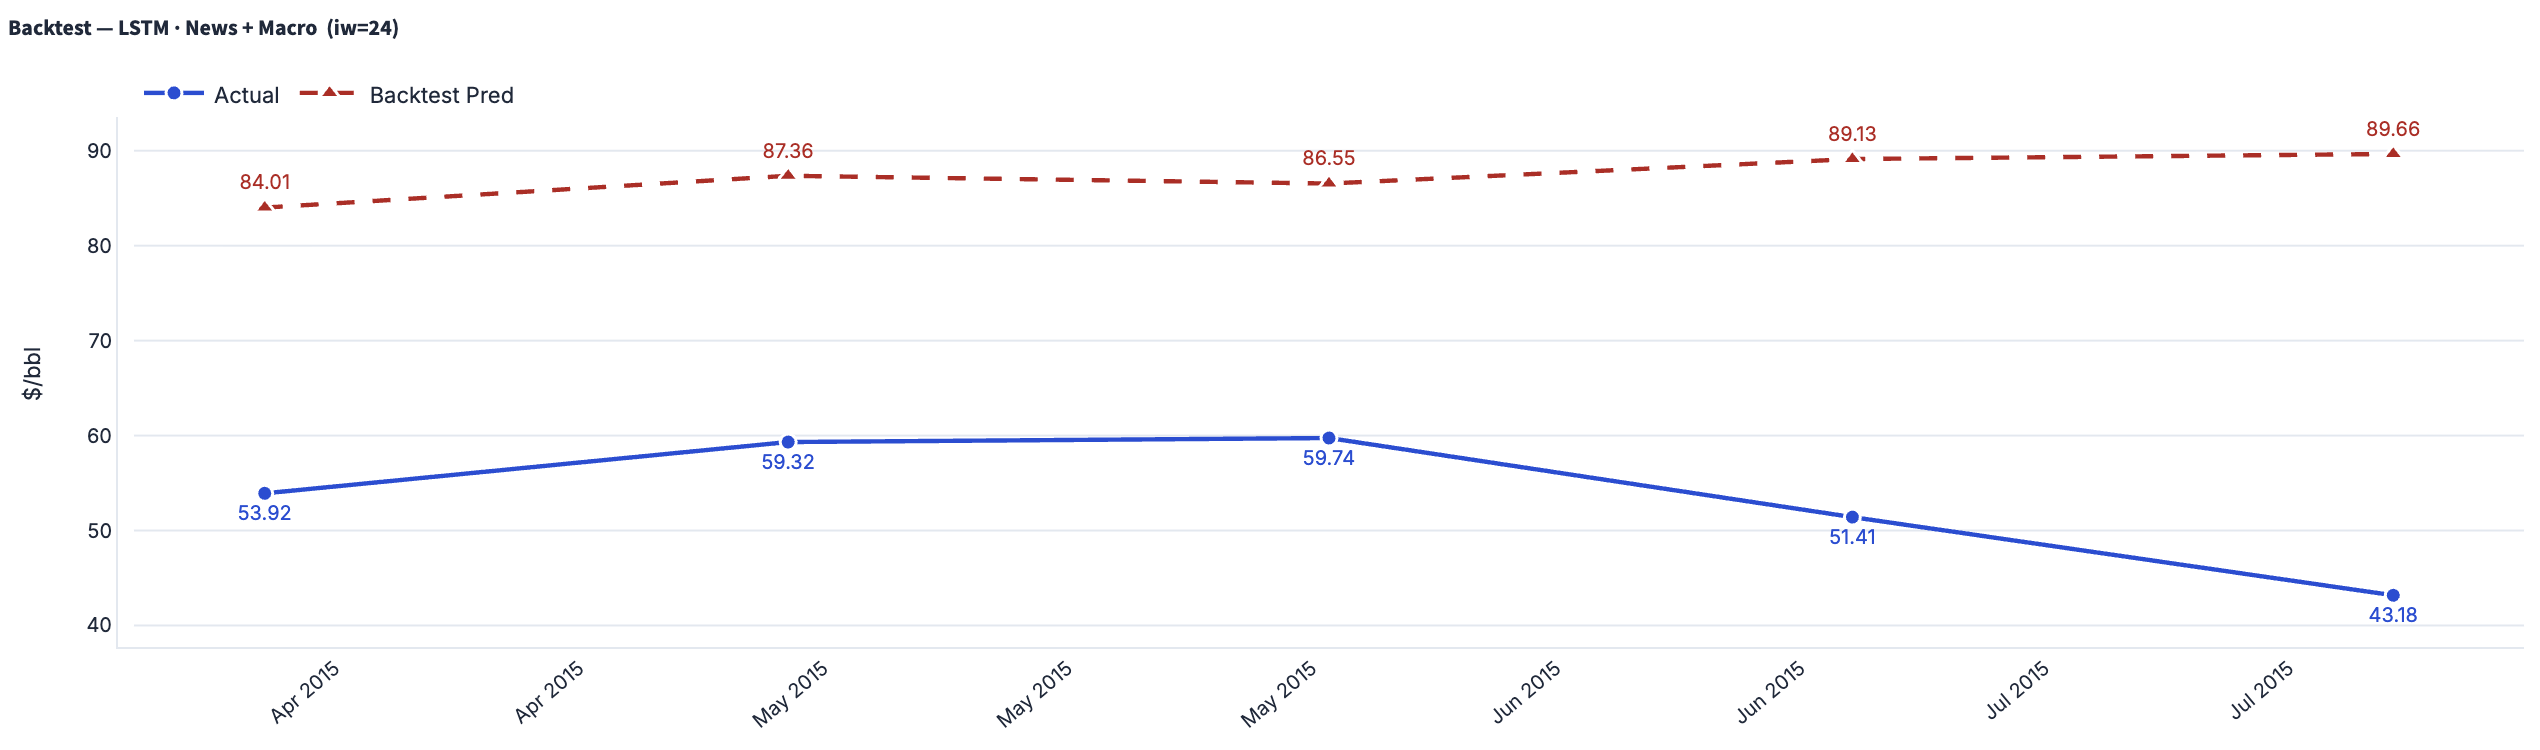
\includegraphics[width=\textwidth]{figures/multivariate_news_macro_oil_lstm_backtest.png}
\small (c) LSTM backtest for crude oil
\end{minipage}\hfill
\begin{minipage}[t]{0.48\textwidth}
\centering
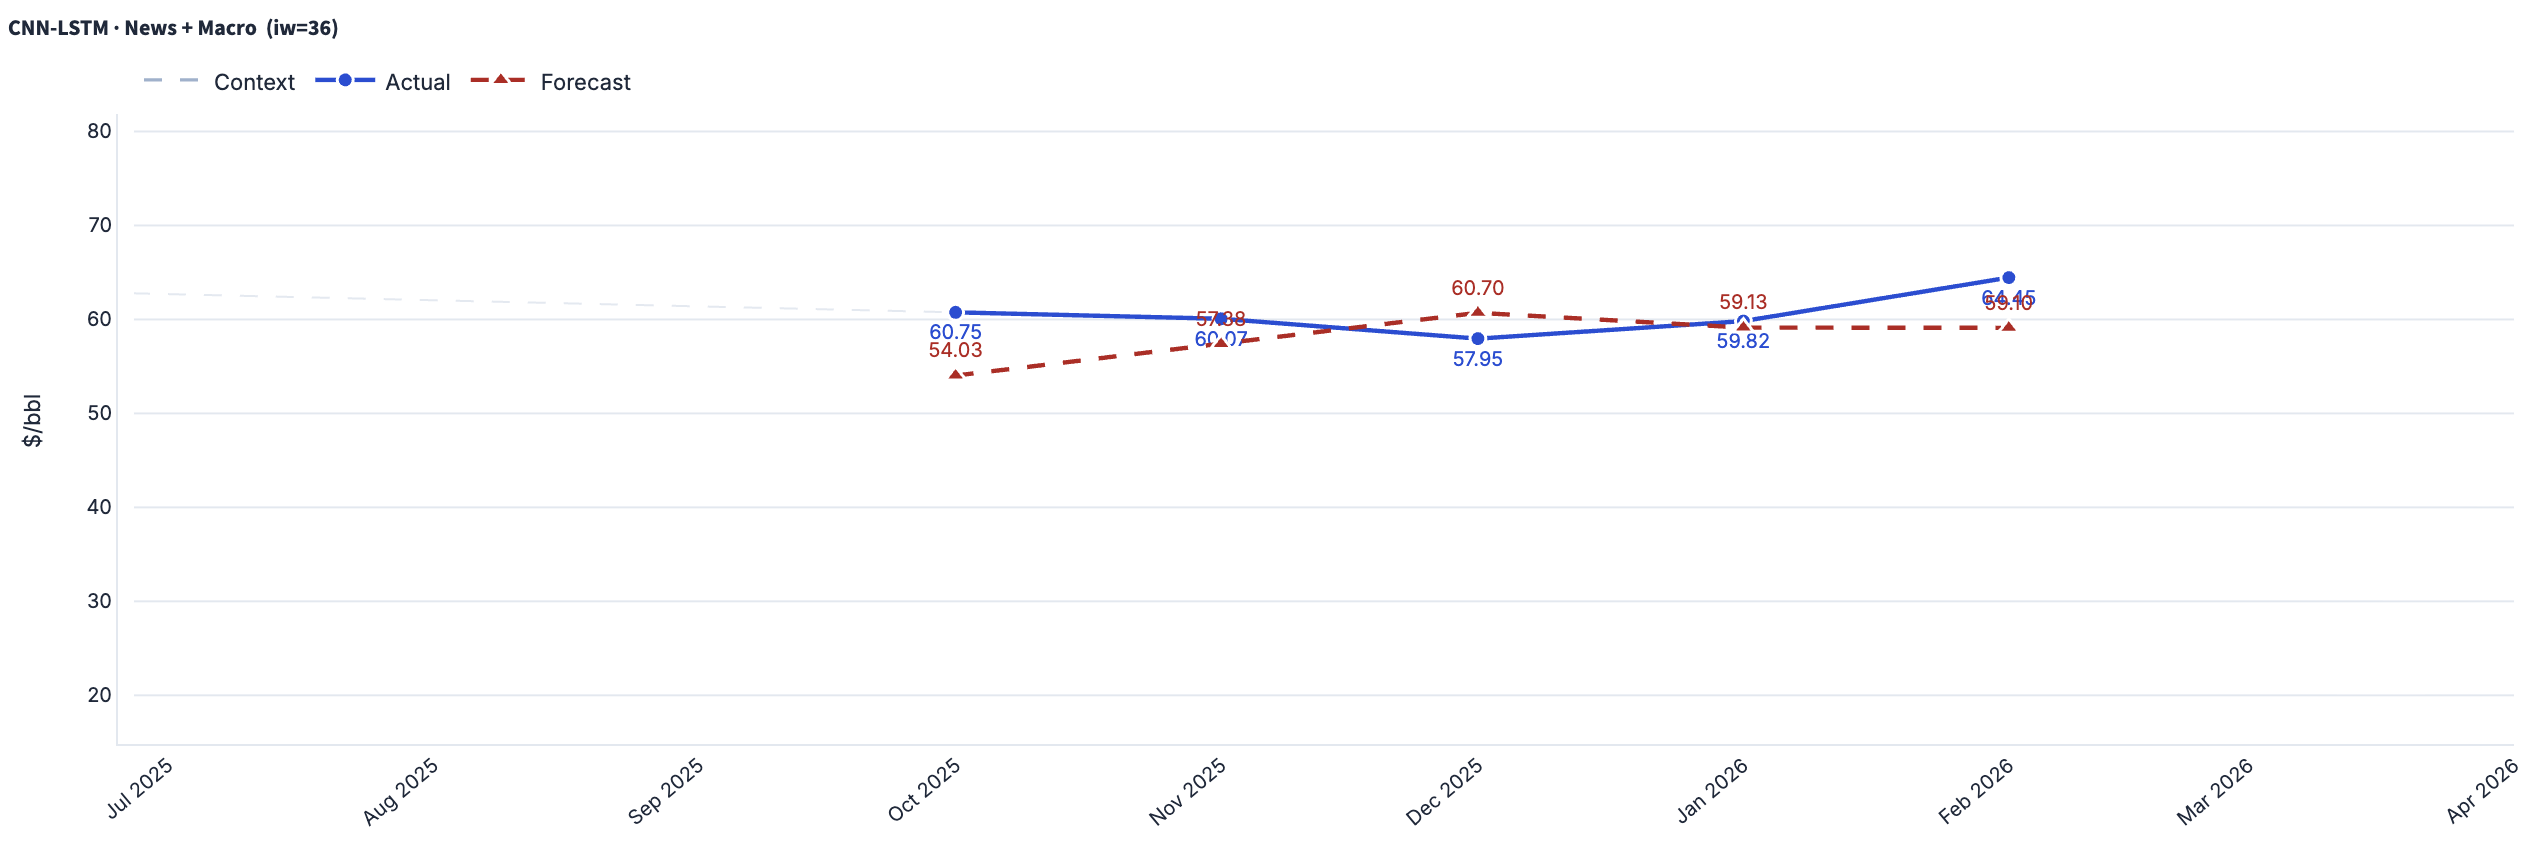
\includegraphics[width=\textwidth]{figures/multivariate_news_macro_oil_cnnlstm.png}
\small (d) CNN--LSTM forecast for crude oil
\end{minipage}

\vspace{0.5em}

\begin{minipage}[t]{0.48\textwidth}
\centering
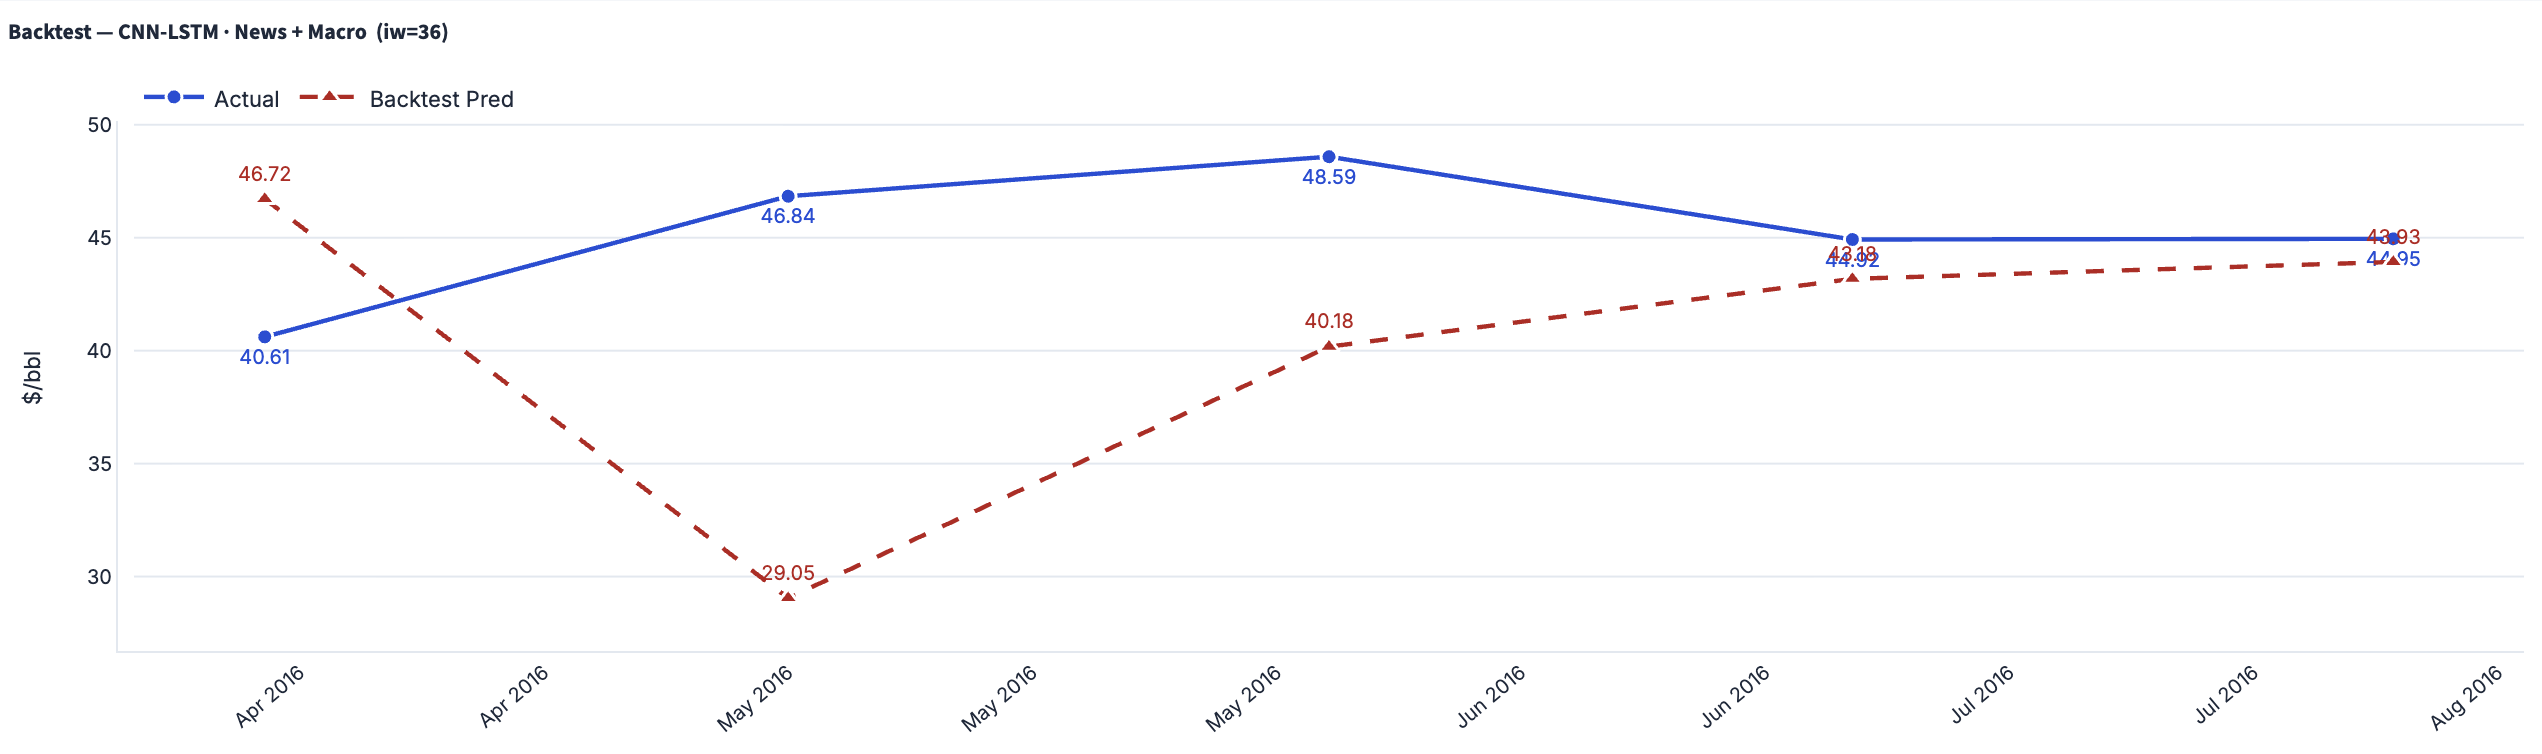
\includegraphics[width=\textwidth]{figures/multivariate_news_macro_oil_cnnlstm_backtest.png}
\small (e) CNN--LSTM backtest for crude oil
\end{minipage}
\caption{Actual versus predicted WTI crude oil prices (USD/barrel) using the combined macroeconomic and GDELT-derived news feature set: (a) SARIMAX forecast, (b) LSTM direct forecast, (c) LSTM walk-forward backtest, (d) CNN--LSTM direct forecast, and (e) CNN--LSTM walk-forward backtest. This figure summarizes the joint-feature multivariate setting.}
\label{fig:combined_oil_plots}
\end{figure}

\begin{table}[h]
\centering
\caption{Combined macro-plus-news model performance for crude oil}
\label{tab:combined_oil}
\begin{tabular}{@{}lcccc@{}}
\toprule
Model & RMSE (USD/barrel) & MAE (USD/barrel) & MAPE (\%) & DA \\
\midrule
SARIMAX & 1.235 & 1.109 & 1.68 & 0.60 \\
LSTM Forecast & 3.200 & 2.631 & 4.25 & 0.40 \\
LSTM Backtest & 34.622 & 33.828 & 65.79 & 0.00 \\
CNN--LSTM Forecast & 4.223 & 3.641 & 5.95 & 0.80 \\
CNN--LSTM Backtest & 9.257 & 7.014 & 15.30 & 0.60 \\
\botrule
\end{tabular}
\end{table}

The combined feature setting leads to a substantial improvement for crude oil, particularly for SARIMAX, which achieves very low error values relative to the previous settings. This suggests that once macroeconomic trends and news signals are used together, the linear model is able to identify substantive relationships that are not visible when either feature group is used in isolation. Figure~\ref{fig:combined_oil_plots} supports this interpretation, as the SARIMAX predictions follow the observed series closely and track the major movements with comparatively little deviation. Directionally, however, the CNN--LSTM forecast attains the highest DA at 0.80, while SARIMAX still remains strong at 0.60.

The LSTM model shows reasonable forecasting performance, but its backtesting error increases sharply, indicating instability across different temporal segments. This pattern suggests that although the model is able to learn useful patterns during training, it struggles to generalize consistently over time; this is also reflected in its backtest DA of 0.00. The CNN--LSTM model performs moderately well in direct forecasting and shows better stability than LSTM, with DA values of 0.80 for the forecast and 0.60 for the backtest, but its performance still remains below that of SARIMAX in RMSE terms. Visually, the neural models tend to generate smoother predictions and show some lag or deviation during periods of abrupt price change.

Overall, the crude-oil results indicate that combining macroeconomic and news-derived features materially improves predictive performance, with SARIMAX benefiting the most from this integration.

\subsubsection*{5.2.3.2 Natural Gas (CNG)}
For natural gas, Table~\ref{tab:combined_cng} reports the combined-feature model performance, and Figure~\ref{fig:combined_cng_plots} shows the associated prediction plots.

\begin{figure}[h]
\centering
\begin{minipage}[t]{0.48\textwidth}
\centering
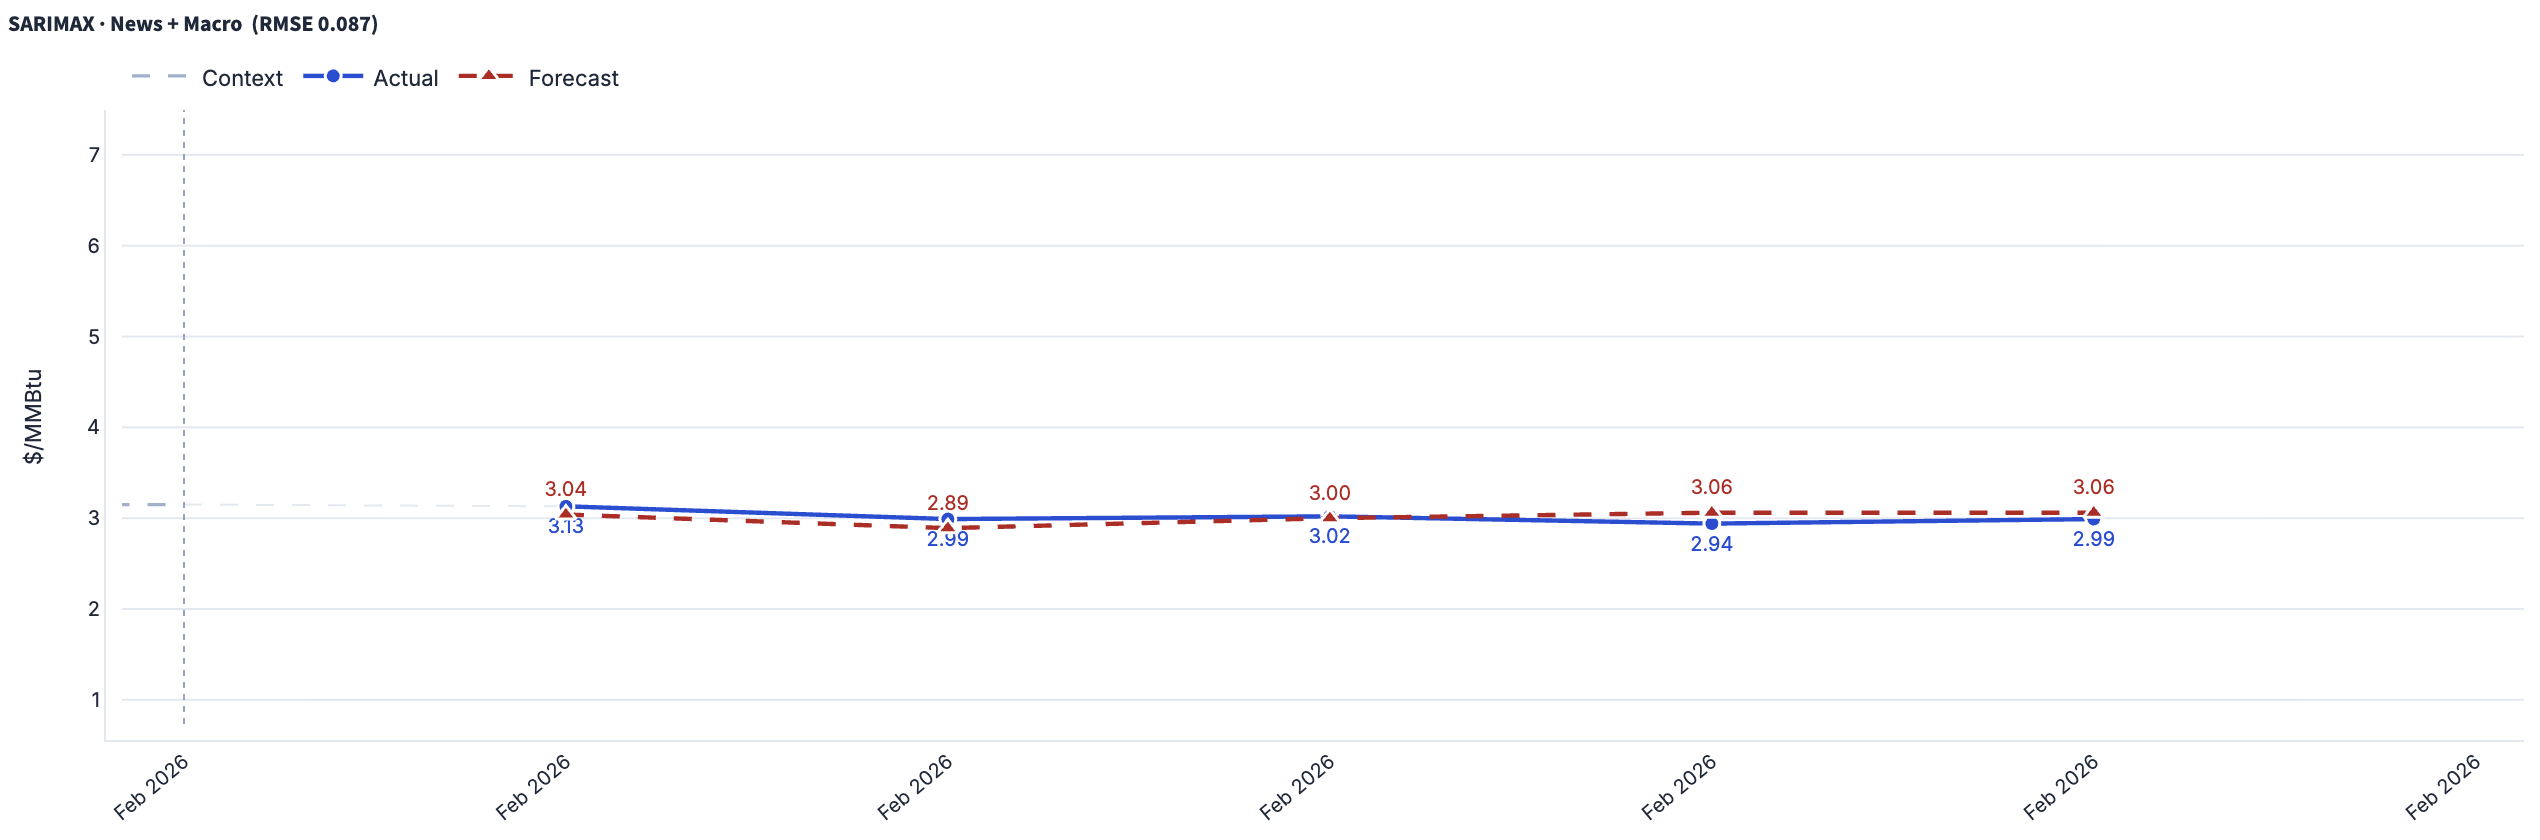
\includegraphics[width=\textwidth]{figures/multivariate_news_macro_cng_sarimax.png}
\small (a) SARIMAX forecast for natural gas
\end{minipage}\hfill
\begin{minipage}[t]{0.48\textwidth}
\centering
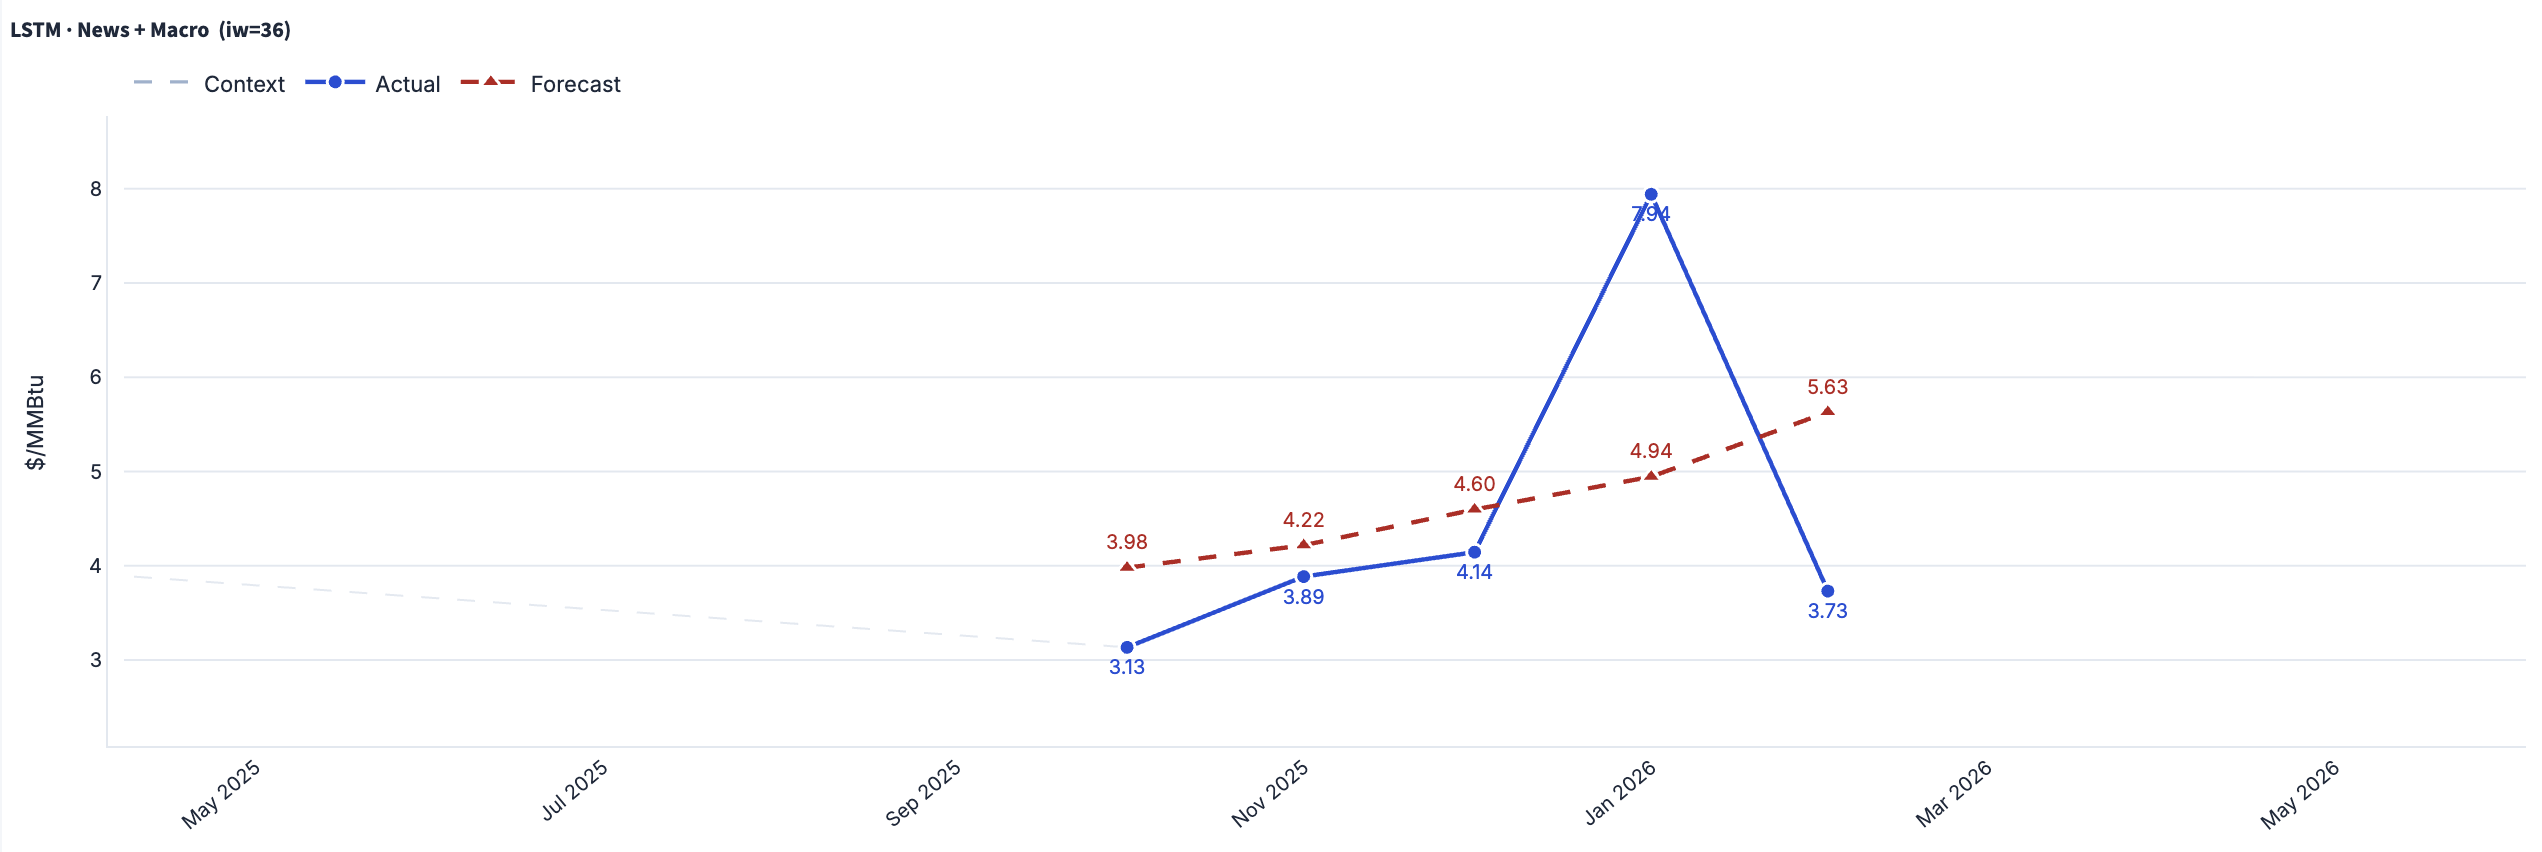
\includegraphics[width=\textwidth]{figures/multivariate_news_macro_cng_lstm.png}
\small (b) LSTM forecast for natural gas
\end{minipage}

\vspace{0.5em}

\begin{minipage}[t]{0.48\textwidth}
\centering
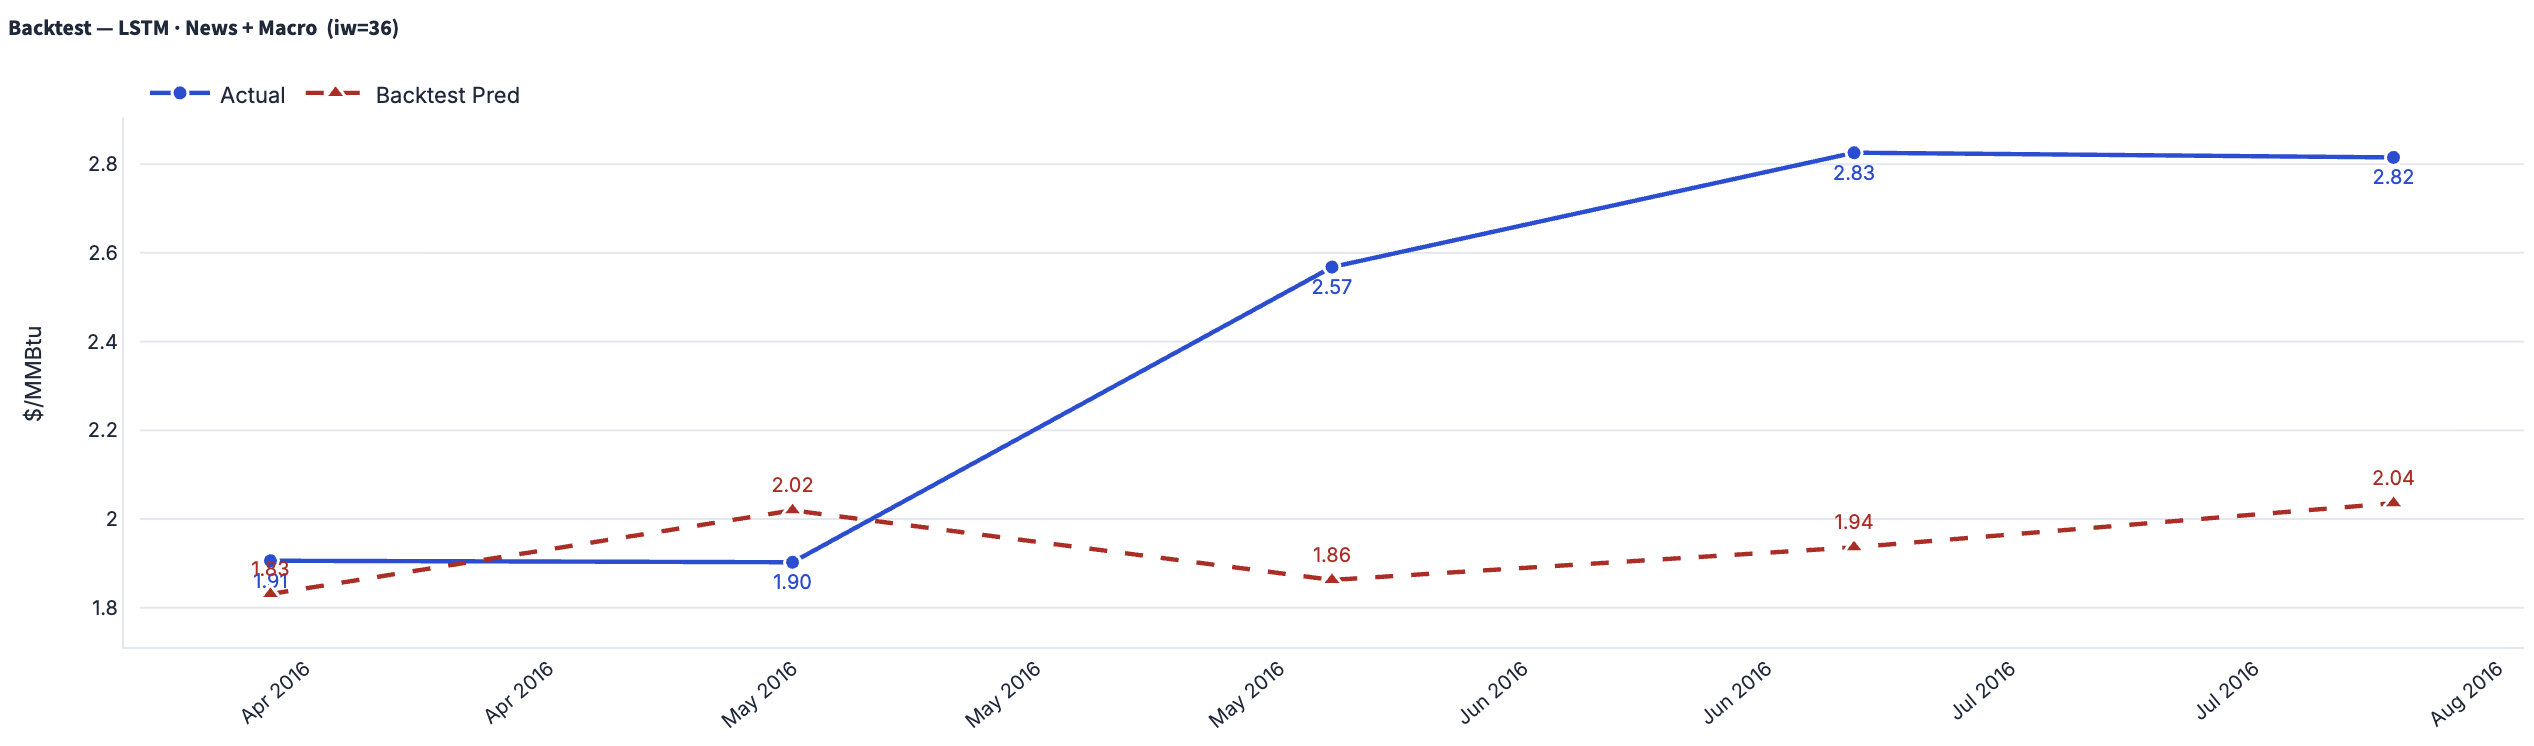
\includegraphics[width=\textwidth]{figures/multivariate_news_macro_cng_lstm_backtest.png}
\small (c) LSTM backtest for natural gas
\end{minipage}\hfill
\begin{minipage}[t]{0.48\textwidth}
\centering
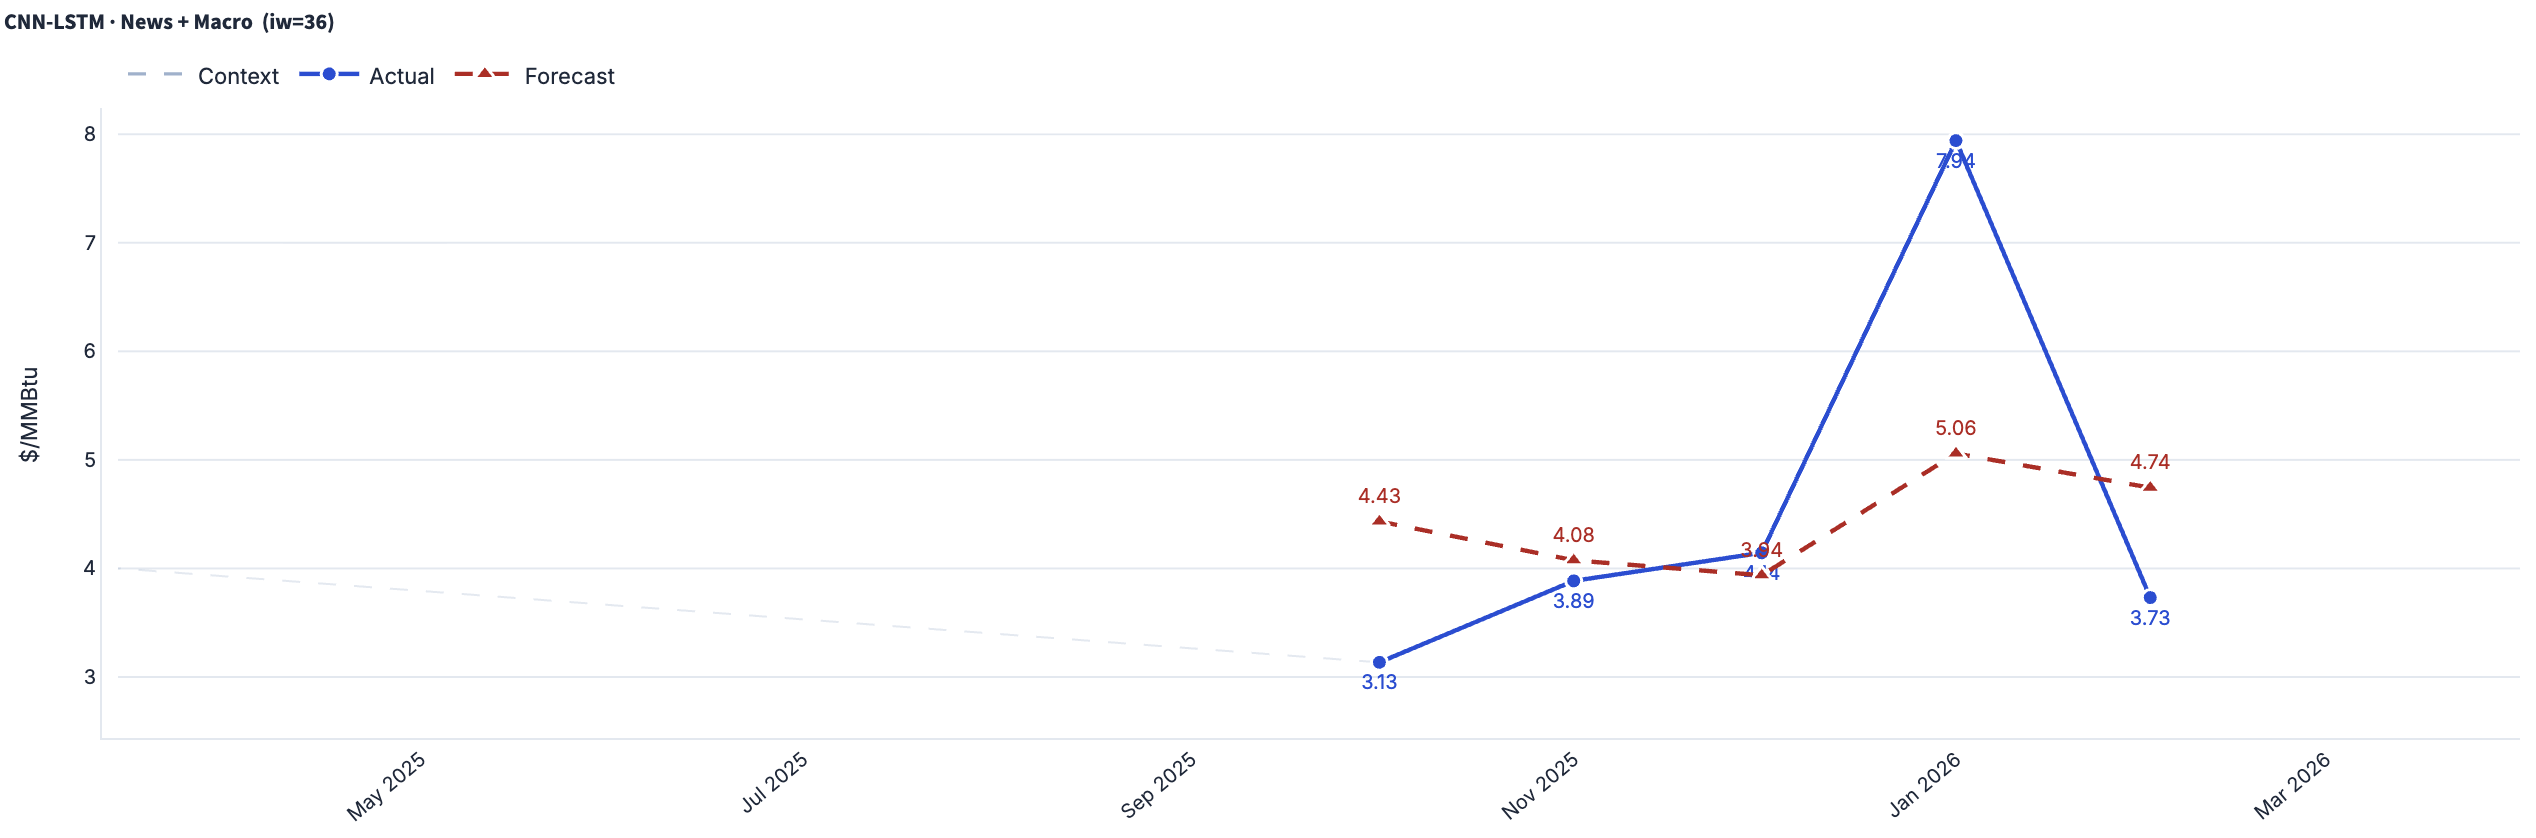
\includegraphics[width=\textwidth]{figures/multivariate_news_macro_cng_cnnlstm.png}
\small (d) CNN--LSTM forecast for natural gas
\end{minipage}

\vspace{0.5em}

\begin{minipage}[t]{0.48\textwidth}
\centering
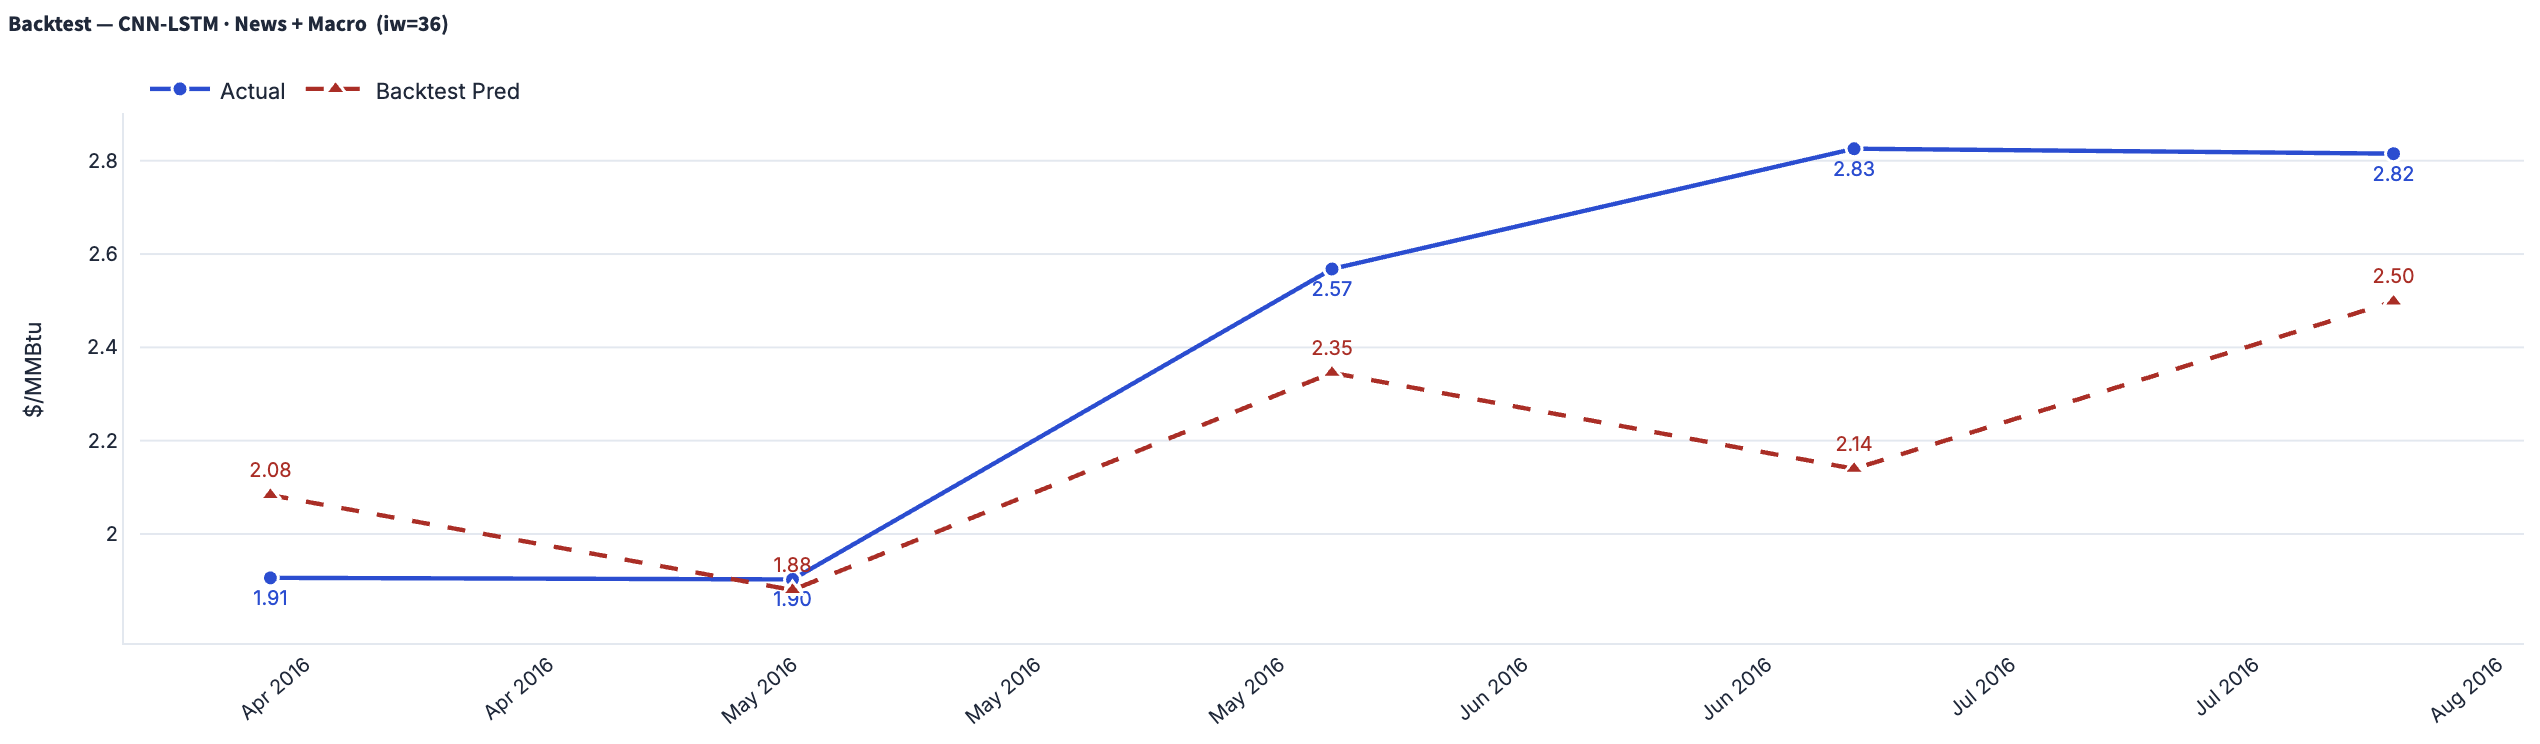
\includegraphics[width=\textwidth]{figures/multivariate_news_macro_cng_cnnlstm_backtest.png}
\small (e) CNN--LSTM backtest for natural gas
\end{minipage}
\caption{Actual versus predicted Henry Hub natural gas prices (USD/MMBtu) using the combined macroeconomic and GDELT-derived news feature set: (a) SARIMAX forecast, (b) LSTM direct forecast, (c) LSTM walk-forward backtest, (d) CNN--LSTM direct forecast, and (e) CNN--LSTM walk-forward backtest. This figure summarizes the joint-feature multivariate setting.}
\label{fig:combined_cng_plots}
\end{figure}

\begin{table}[h]
\centering
\caption{Combined macro-plus-news model performance for natural gas}
\label{tab:combined_cng}
\begin{tabular}{@{}lcccc@{}}
\toprule
Model & RMSE (USD/MMBtu) & MAE (USD/MMBtu) & MAPE (\%) & DA \\
\midrule
SARIMAX & 0.087 & 0.080 & 2.66 & 0.80 \\
LSTM Forecast & 1.650 & 1.305 & 27.01 & 0.40 \\
LSTM Backtest & 0.619 & 0.513 & 19.34 & 0.25 \\
CNN--LSTM Forecast & 1.490 & 1.118 & 22.95 & 0.60 \\
CNN--LSTM Backtest & 0.361 & 0.285 & 10.94 & 0.40 \\
\botrule
\end{tabular}
\end{table}

For natural gas, the combined setting shows comparatively lower error values than the macro-only and news-only setups. The SARIMAX results suggest that the joint feature space represents part of the variation in this series more effectively when macroeconomic and news-based inputs are used together. Compared with the earlier settings, the predictions in Figure~\ref{fig:combined_cng_plots} align more closely with the observed values, particularly in terms of direction and broad magnitude of change. This is reflected in the DA values as well, with SARIMAX reaching 0.80 and CNN--LSTM forecast reaching 0.60.

Unlike the crude-oil case, the neural models also show comparatively more consistent forecasting and backtesting behavior. This is especially visible for CNN--LSTM, whose backtest error for natural gas is lower than its corresponding crude-oil result, suggesting that the combined macro-plus-news inputs are relatively more useful for CNG in this architecture. Although the neural models remain less accurate than SARIMAX in absolute terms, they appear comparatively more stable here than in the isolated feature settings; even so, their DA values remain below the SARIMAX benchmark.

Taken together, the combined-model results suggest that integrating macroeconomic indicators with news-derived signals is comparatively more useful than using either source alone. The macro-only models struggled to track short-term variations, while the news-only models lacked stability and precision. By comparison, the combined models are more able to connect structured trends with event-driven information. SARIMAX shows the lowest errors in this setting, while the neural models, especially CNN--LSTM for CNG, also look comparatively better than in the separate feature settings, even though they still face challenges in reproducing extreme fluctuations.

\begin{table}[h]
\centering
\small
\caption{Best-performing model by setting and commodity}
\label{tab:summary_best_models}
\begin{tabular}{@{}p{1.5cm}p{1.8cm}p{0.8cm}p{1.8cm}p{0.7cm}p{3.8cm}@{}}
\toprule
Commodity & Lowest-RMSE Model & RMSE & Best-DA Model & DA & Interpretation \\
\midrule
Crude oil & SARIMAX & 1.235 & CNN--LSTM Forecast & 0.80 & In the combined setting, SARIMAX yields the lowest RMSE, whereas CNN--LSTM provides the strongest directional signal for crude oil. \\
Natural gas & SARIMAX & 0.087 & SARIMAX & 0.80 & In the combined setting, SARIMAX achieves both the lowest RMSE and the highest directional accuracy for natural gas. \\
\botrule
\end{tabular}
\end{table}

\section{Discussion}\label{sec12}

The experimental results reveal that predictive performance is strongly contingent on both the nature of the exogenous information incorporated and the commodity under examination - a finding that reflects the fundamentally different price formation processes governing crude oil and natural gas markets. In the macro-only setting, predictive performance remains uneven because broad economic indicators evolve more slowly than commodity prices and therefore explain medium-term conditions better than abrupt short-term moves. This structural mismatch between the low-frequency dynamics of macroeconomic variables and the higher-frequency movements of commodity prices helps explain why macro-only models can detect broad directional regime shifts while nonetheless failing to resolve the timing and magnitude of localized price shocks.

The news-only setting highlights a different trade-off. GDELT-based features contain relevant event information, but the aggregation process also introduces noise by compressing heterogeneous news into summary measures such as event counts, tone, and conflict intensity. As a result, news-only models can identify broad directional changes but often remain unstable, especially for natural gas, where sharp price movements are difficult to infer from aggregated event signals alone.

The combined macro-plus-news setting performs best because it brings together slower-moving structural context and faster-moving event-driven information. In this setting, SARIMAX benefits most, suggesting that once the feature space is enriched, a well-specified linear model can exploit substantive explanatory relationships without requiring highly flexible nonlinear dynamics. The neural models also improve under the combined setup, but they continue to produce smoother outputs and show weaker robustness during abrupt market changes, indicating that additional data or architecture refinement is still needed for consistent gains.

Overall, the findings suggest that exogenous variables are most valuable as complementary signals rather than as isolated substitutes for price history. The main contribution of macroeconomic and news-based inputs is not perfect point forecasting, but improved directional understanding, better turning-point detection, and a more interpretable view of which external conditions coincide with changing energy prices.

\section{Limitations and Future Work}\label{sec14}

Energy price forecasting remains challenging due to the complex interplay of economic, geopolitical, and market-specific factors, many of which are not fully represented by the selected macroeconomic indicators and aggregated news signals. While these inputs provide useful context, they may fail to represent sudden shocks or localized events that drive sharp price movements. Additionally, classical time series models are inherently linear and may not fully model nonlinear relationships, while neural network models, although more flexible, tend to produce smoother outputs and may struggle to respond to high volatility and abrupt changes in the data.

A further limitation pertains to the representational granularity of the news data. The use of aggregated GDELT features improves computational efficiency but reduces the granularity of event-level information, potentially limiting the richness of extracted signals. Furthermore, the inherent noise and variability in energy price series, particularly in natural gas markets, can affect model stability and generalization across different time periods, leading to inconsistent performance under different conditions.

Future work can address these limitations by expanding both the feature space and modeling strategies. This includes testing models with additional macroeconomic variables that are indirectly correlated with energy prices, which may reflect hidden economic influences. Future work could substantially improve the quality and specificity of news-based signals by replacing aggregated GDELT summary statistics with richer natural language representations - such as transformer-derived sentence embeddings (e.g., BERT, FinBERT) - applied directly to the source text of relevant news articles. Further, modeling the temporal impact of events, including how long a news event influences prices through temporal weighting mechanisms, can provide deeper insight into market behavior. Finally, exploring more advanced architectures, such as attention-based or transformer models, may improve the ability to model complex dependencies and enhance overall forecasting performance.


\section{Conclusion}\label{sec13}

This study investigated the extent to which macroeconomic indicators sourced from the FRED database and event-driven news signals derived from the GDELT repository can improve the forecasting accuracy and directional tracking of WTI crude oil and Henry Hub natural gas prices. Across the experiments, the combined macro-plus-news setting generally performed better than the macro-only and news-only alternatives, indicating that structured economic signals and event-driven information reflect complementary aspects of energy price behavior.

The findings suggest that GDELT-based features and macroeconomic variables can help detect broad market direction and relevant shifts in oil and gas prices, even when the models do not track future fluctuations with high precision. In particular, the combined-feature SARIMAX models delivered the most reliable overall performance in this study, suggesting that the joint feature space may contain substantive explanatory relationships that are less visible in isolated settings. Neural architectures such as LSTM and CNN--LSTM were also able to model parts of the underlying dynamics, but their forecasting and backtesting performance remained less stable, especially during periods of abrupt price change.

Taken together, the empirical results indicate that incorporating heterogeneous exogenous information can improve directional energy price modeling and, in some settings, reduce forecast error in well-specified linear frameworks. At the same time, precise short-term point forecasting of volatile commodity prices remains difficult. Energy markets are influenced by rapidly changing geopolitical events, structural breaks, and nonlinear interactions that are not fully represented by aggregated macroeconomic indicators or news summaries alone. For this reason, the proposed framework should be viewed as a comparative and exploratory step toward richer predictive modeling rather than as a complete or universally superior solution.

From a research perspective, this study contributes a comparative framework for evaluating univariate and multivariate models under a consistent validation setting, while also showing the conditional value of combining structured macroeconomic variables with event-driven news features. The explicit limitations discussed in Section~\ref{sec14} are therefore central to interpreting the results: the gains reported here depend on the selected features, model classes, and evaluation design, and they should be read as evidence of useful signal rather than definitive predictive dominance.

%%===========================================================================================%%
%% References included directly in the manuscript file                                      %%
%%===========================================================================================%%

\begin{thebibliography}{28}

\bibitem{akaike1974}
Akaike, H.: A new look at the statistical model identification. IEEE Transactions on Automatic Control \textbf{19}(6), 716--723 (1974).

\bibitem{akiba2019optuna}
Akiba, T., Sano, S., Yanase, T., Ohta, T., Koyama, M.: Optuna: A next-generation hyperparameter optimization framework. In: Proceedings of the 25th ACM SIGKDD International Conference on Knowledge Discovery and Data Mining, pp. 2623--2631 (2019).

\bibitem{baker2016}
Baker, S.R., Bloom, N., Davis, S.J.: Measuring economic policy uncertainty. The Quarterly Journal of Economics \textbf{131}(4), 1593--1636 (2016).

\bibitem{baumeister2016}
Baumeister, C., Kilian, L.: Forty years of oil price fluctuations: why the price of oil may still surprise us. Journal of Economic Perspectives \textbf{30}(1), 139--160 (2016).

\bibitem{box1976}
Box, G.E.P., Jenkins, G.M.: \textit{Time Series Analysis: Forecasting and Control}. Holden-Day, San Francisco (1976).

\bibitem{busari2021}
Busari, G.A., Lim, D.H.: Crude oil price prediction: a comparison between AdaBoost-LSTM and AdaBoost-GRU for improving forecasting performance. Computers \& Chemical Engineering \textbf{155}, 107513 (2021).

\bibitem{cen2019}
Cen, Z., Wang, J.: Crude oil price prediction model with long short-term memory deep learning based on prior knowledge data transfer. Energy \textbf{169}, 160--171 (2019).

\bibitem{dickey1979}
Dickey, D.A., Fuller, W.A.: Distribution of the estimators for autoregressive time series with a unit root. Journal of the American Statistical Association \textbf{74}(366), 427--431 (1979).

\bibitem{diebold1995}
Diebold, F.X., Mariano, R.S.: Comparing predictive accuracy. Journal of Business \& Economic Statistics \textbf{13}(3), 253--263 (1995).

\bibitem{durbin2012}
Durbin, J., Koopman, S.J.: \textit{Time Series Analysis by State Space Methods}, 2nd edn. Oxford University Press, Oxford (2012).

\bibitem{fred2025}
Federal Reserve Bank of St. Louis: Federal Reserve Economic Data (FRED). \url{https://fred.stlouisfed.org/} (accessed 2025).

\bibitem{gers2000}
Gers, F.A., Schmidhuber, J., Cummins, F.: Learning to forget: continual prediction with LSTM. Neural Computation \textbf{12}(10), 2451--2471 (2000).

\bibitem{goldstein1992}
Goldstein, J.S.: A conflict-cooperation scale for WEIS events data. Journal of Conflict Resolution \textbf{36}(2), 369--385 (1992).

\bibitem{hamilton2003}
Hamilton, J.D.: What is an oil shock? Journal of Econometrics \textbf{113}(2), 363--398 (2003).

\bibitem{hamilton2009}
Hamilton, J.D.: Causes and consequences of the oil shock of 2007--08. Brookings Papers on Economic Activity \textbf{2009}(1), 215--261 (2009).

\bibitem{hochreiter1997}
Hochreiter, S., Schmidhuber, J.: Long short-term memory. Neural Computation \textbf{9}(8), 1735--1780 (1997).

\bibitem{huber1964}
Huber, P.J.: Robust estimation of a location parameter. Annals of Mathematical Statistics \textbf{35}(1), 73--101 (1964).

\bibitem{hyndman2018}
Hyndman, R.J., Athanasopoulos, G.: \textit{Forecasting: Principles and Practice}, 2nd edn. OTexts, Melbourne (2018).

\bibitem{kilian2009}
Kilian, L.: Not all oil price shocks are alike: disentangling demand and supply shocks in the crude oil market. American Economic Review \textbf{99}(3), 1053--1069 (2009).

\bibitem{kim2018}
Kim, H.Y., Won, C.H.: Forecasting the volatility of stock price index: a hybrid model integrating LSTM with multiple GARCH-type models. Expert Systems with Applications \textbf{103}, 25--37 (2018).

\bibitem{kingma2015}
Kingma, D.P., Ba, J.: Adam: a method for stochastic optimization. In: International Conference on Learning Representations (2015).

\bibitem{kwiatkowski1992}
Kwiatkowski, D., Phillips, P.C.B., Schmidt, P., Shin, Y.: Testing the null hypothesis of stationarity against the alternative of a unit root. Journal of Econometrics \textbf{54}(1--3), 159--178 (1992).

\bibitem{lecun1998}
LeCun, Y., Bottou, L., Bengio, Y., Haffner, P.: Gradient-based learning applied to document recognition. Proceedings of the IEEE \textbf{86}(11), 2278--2324 (1998).

\bibitem{leetaru2013}
Leetaru, K., Schrodt, P.A.: GDELT: Global Data on Events, Location, and Tone, 1979--2012. In: ISA Annual Convention (2013).

\bibitem{li2014}
Li, X., Xie, H., Chen, L., Wang, J., Deng, X.: News impact on stock price return via sentiment analysis. Knowledge-Based Systems \textbf{69}, 14--23 (2014).

\bibitem{sainath2015}
Sainath, T.N., Vinyals, O., Senior, A., Sak, H.: Convolutional, long short-term memory, fully connected deep neural networks. In: Proceedings of the IEEE International Conference on Acoustics, Speech and Signal Processing (ICASSP), pp. 4580--4584 (2015).

\bibitem{shapiro2022}
Shapiro, A.H., Sudhof, M., Wilson, D.J.: Measuring news sentiment. Journal of Econometrics \textbf{228}(2), 221--243 (2022).

\bibitem{tetlock2007}
Tetlock, P.C.: Giving content to investor sentiment: the role of media in the stock market. The Journal of Finance \textbf{62}(3), 1139--1168 (2007).

\end{thebibliography}

\end{document}
